%
% thesis.tex
%
% Master's Thesis/Ph.D. Dissertation Template
% Clemson University
%

%
% The document guidelines say the font can be between 10pt and 12pt.
% Specify whatever you want it to be here.
%
\documentclass[10pt]{ClemsonThesis}

%
% Use any additional packages you might need
%
%% \usepackage{listings}
%% \usepackage{comment}
\usepackage{fancyhdr}
\usepackage{array,booktabs}
\usepackage{multirow}
\usepackage{graphicx}
\usepackage{caption}
\usepackage{subcaption}
\usepackage{comment}
\usepackage{appendix}
\usepackage{color}
\usepackage{balance}
\usepackage{arydshln}
\usepackage[normalem]{ulem}
\usepackage{threeparttable}
\usepackage{xcolor}
%\usepackage{ntheorem}

\newtheorem{theorem}{RQ}
%\usepackage{chngcntr}
%\newcounter{pretheorem}
%\counterwithin{theorem}{pretheorem}
%
%\renewcommand\thetheorem{\arabic{pretheorem}\alph{theorem}}
%\newcommand{\theoremgroup}{\refstepcounter{pretheorem}}
%
% Make the document your own -- fill in these values to reflect the type of
% document you are writing.
%
\title{%A Data-Driven Approach to 
	Recommending Privacy Settings for Internet-of-Things}
\department{School of Computing}
\documentType{Dissertation}
\major{Computer Science}
\degree{Doctor of Philosophy}
\graduationMonth{Dec}
\graduationYear{2019}
\author{Yang He}
\committeeChair{Dr. Bart P. Knijnenburg}
\committeeMemberOne{Dr. Larry F. Hodges}
\committeeMemberTwo{Dr. Alexander Herzog}
\committeeMemberThree{Dr. Ilaria Torre}

%% optional (for Master's) \committeeMemberThree{Dr. John Doe}
%% optional \committeeMemberFour{Dr. Jane Doe}
%% optional \committeeMemberFive{Dr. Mary Doe}
%% optional \committeeMemberSix{Dr. Mark Doe}

%
% PDF Setup -- most of this you do not need to touch
%
\hypersetup{
	colorlinks,
	linkcolor={black},
	citecolor={black},
	filecolor={black},
	urlcolor={black},
	pdftitle={\theTitle},
	pdfauthor={\theAuthor},
	pdfsubject={\theDocumentType},
	pdfkeywords={Clemson University, \theDepartment, \theDocumentType, \theMajor, \theDegree},
	pdfstartpage={1},
}


%
% User-specified command definitions/redefinitions
%
%% \newcommand{\cplusplus}{{\rm C\raise.5ex\hbox{\small ++}}}
%% \newcommand{\num}[1]{\mbox{(\textit{#1})}}
%% \renewcommand{\ttdefault}{pcr}
%% \renewcommand\lstlistlistingname{List of Listings}
\pagestyle{fancy}
\lhead{Yang He}
\rhead{Dissertation}
\renewcommand{\headrulewidth}{0.4pt}
\renewcommand*\contentsname{Outline}

\begin{document}
	%  ============================================================================
	\frontmatter % Begin front matter (pages are numbered with Roman numerals)
	%  ============================================================================
	
	\maketitle          % Generate the title page
	
	\doublespacing                             % Text should be double spaced
	\setcounter{page}{2}                       % Abstract begins on page 2
	\addtotoc{Abstract}{\chapter*{Abstract}
The rapidly accelerating growth of these Internet of Things (IoT) technologies brings huge social and economic impact in many fields. However, the rise of IoT also comes with a number of privacy risks, including facilitation of the collection of large amounts of consumer data, processing and storing the data in ways unexpected by the consumer, and privacy and security breach.

Prior research has shown that privacy issues are the underlying obstacles to the adoption of social and mobile technologies. Privacy concerns have been identified as an important barrier to the growth of IoT. This is also true when it comes to the domain of setting privacy for IoT devices. The user interface for setting privacy preference of present IoT device is imperfect even for a smartphone, not to mention the complexity of manually setting privacy preferences for numerous different other IoT devices. Hence, there is a demand to solve the following, urgent research question: How can we help users simplify the task of controlling privacy setting for IoT devices in a user-friendly manner, so that they can make good privacy decisions?

Existing solutions to this problem in other domains involve giving users more control over, and information about the privacy settings provided by the systems as well as privacy nudges. However, neither of them work well in the IoT domain. Providing transparency and control does give users the freedom of managing their privacy in IoT according to their own privacy decisions, but privacy decision making is often not rational. Thus, such extra transparency and control may increase the difficulty of setting appropriate privacy for users. Privacy nudges are usually implemented in the form of prompts, which will create constant noises given that the IoT systems usually work in the background. At the same time, they lack the personalization to the inherent diversity of users’ privacy preferences and the context-dependency of their decisions.

To solve these problems in the IoT domain, a more fundamental understanding of the logic behind IoT users' privacy decisions in different IoT contexts is needed. We therefore conducted a series of studies to contextualize the IoT users' decision making characteristics, and designed a set of privacy-setting interfaces to help them manage their privacy settings in various IoT contexts based on the deeper understanding of users' privacy decision behaviors. 

In this proposal, we first present three studies on recommending privacy settings for different IoT environments, namely general/public IoT, household IoT, and fitness IoT, respectively. We developed and utilized a `` data-driven" approach in these three studies -- We first use statistical analysis and machine learning techniques on the collected user data to gain the underlying insights of IoT users' privacy decision behavior; and then create a set of ``smart" privacy defaults/profiles based on these insights. Finally, we design a set of interfaces to incorporate these privacy default/profiles. Users can apply these smart defaults/profiles by either a single click or by answering a few related questions.

Our current biggest limitation for such ``data-driven" approach is that we did not test any of the presented interfaces, so we do not know what level of complexity (both in terms of the user interface and the in terms of the profiles) is most suitable. Thus for my proposed work, I will address this limitation by discussing our proposed study to evaluate the new interfaces of recommending privacy-settings for household IoT. Our research can benefit the IoT users, manufacturers, and researchers, privacy-setting interface designers and anyone who has or want to adopt IoT devices.
}  % Generate the abstract
	
    %
	% The dedication page is optional.  Comment out this line if you do not
	% want to include this page.
	%
	\addtotoc{Dedication}{\chapter*{Dedication}
Lorem ipsum dolor sit amet, consetetur sadipscing elitr,  sed diam nonumy eirmod
tempor invidunt ut labore et dolore magna aliquyam erat, sed diam voluptua. At
vero eos et accusam et justo duo dolores et ea rebum. Stet clita kasd gubergren,
no sea takimata sanctus est Lorem ipsum dolor sit amet. Lorem ipsum dolor sit
amet, consetetur sadipscing elitr,  sed diam nonumy eirmod tempor invidunt ut
labore et dolore magna aliquyam erat, sed diam voluptua. At vero eos et accusam
et justo duo dolores et ea rebum. Stet clita kasd gubergren, no sea takimata
sanctus est Lorem ipsum dolor sit amet. Lorem ipsum dolor sit amet, consetetur
sadipscing elitr,  sed diam nonumy eirmod tempor invidunt ut labore et dolore
magna aliquyam erat, sed diam voluptua. At vero eos et accusam et justo duo
dolores et ea rebum. Stet clita kasd gubergren, no sea takimata sanctus est
Lorem ipsum dolor sit amet.
}
	
	%
	% The acknowledgment page is optional.  Comment out this line if you do
	% not want to include this page.
	%
	\addtotoc{Acknowledgments}{\chapter*{Acknowledgments}
Lorem ipsum dolor sit amet, consetetur sadipscing elitr,  sed diam nonumy eirmod
tempor invidunt ut labore et dolore magna aliquyam erat, sed diam voluptua. At
vero eos et accusam et justo duo dolores et ea rebum. Stet clita kasd gubergren,
no sea takimata sanctus est Lorem ipsum dolor sit amet. Lorem ipsum dolor sit
amet, consetetur sadipscing elitr,  sed diam nonumy eirmod tempor invidunt ut
labore et dolore magna aliquyam erat, sed diam voluptua. At vero eos et accusam
et justo duo dolores et ea rebum. Stet clita kasd gubergren, no sea takimata
sanctus est Lorem ipsum dolor sit amet. Lorem ipsum dolor sit amet, consetetur
sadipscing elitr,  sed diam nonumy eirmod tempor invidunt ut labore et dolore
magna aliquyam erat, sed diam voluptua. At vero eos et accusam et justo duo
dolores et ea rebum. Stet clita kasd gubergren, no sea takimata sanctus est
Lorem ipsum dolor sit amet.

Duis autem vel eum iriure dolor in hendrerit in vulputate velit esse molestie
consequat, vel illum dolore eu feugiat nulla facilisis at vero eros et accumsan
et iusto odio dignissim qui blandit praesent luptatum zzril delenit augue duis
dolore te feugait nulla facilisi. Lorem ipsum dolor sit amet, consectetuer
adipiscing elit, sed diam nonummy nibh euismod tincidunt ut laoreet dolore
magna aliquam erat volutpat.

Ut wisi enim ad minim veniam, quis nostrud exerci tation ullamcorper suscipit
lobortis nisl ut aliquip ex ea commodo consequat. Duis autem vel eum iriure
dolor in hendrerit in vulputate velit esse molestie consequat, vel illum dolore
eu feugiat nulla facilisis at vero eros et accumsan et iusto odio dignissim qui
blandit praesent luptatum zzril delenit augue duis dolore te feugait nulla
facilisi.

Nam liber tempor cum soluta nobis eleifend option congue nihil imperdiet doming
id quod mazim placerat facer possim assum. Lorem ipsum dolor sit amet,
consectetuer adipiscing elit, sed diam nonummy nibh euismod tincidunt ut laoreet
dolore magna aliquam erat volutpat. Ut wisi enim ad minim veniam, quis nostrud
exerci tation ullamcorper suscipit lobortis nisl ut aliquip ex ea commodo
consequat.

Duis autem vel eum iriure dolor in hendrerit in vulputate velit esse molestie
consequat, vel illum dolore eu feugiat nulla facilisis.

At vero eos et accusam et justo duo dolores et ea rebum. Stet clita kasd
gubergren, no sea takimata sanctus est Lorem ipsum dolor sit amet. Lorem ipsum
dolor sit amet, consetetur sadipscing elitr,  sed diam nonumy eirmod tempor
invidunt ut labore et dolore magna aliquyam erat, sed diam voluptua. At vero
eos et accusam et justo duo dolores et ea rebum. Stet clita kasd gubergren, no
sea takimata sanctus est Lorem ipsum dolor sit amet. Lorem ipsum dolor sit
amet, consetetur sadipscing elitr,  At accusam aliquyam diam diam dolore
dolores duo eirmod eos erat, et nonumy sed tempor et et invidunt justo labore
Stet clita ea et gubergren, kasd magna no rebum. sanctus sea sed takimata ut
vero voluptua. est Lorem ipsum dolor sit amet. Lorem ipsum dolor sit amet,
consetetur sadipscing elitr,  sed diam nonumy eirmod tempor invidunt ut labore
et dolore magna aliquyam erat. 
}
	
	\singlespacing                             % Single space the lists
	\tableofcontents \clearpage                % Generate the Table of Contents               

	\addtotoc{List of Tables}{\listoftables}   % Generate the List of Tables
	\addtotoc{List of Figures}{\listoffigures} % Generate the List of Figures
	%\addtotoc{List of Listings}{\lstlistoflistings}
	

	%\addtotoc{Abstract}{\chapter*{Abstract}
The rapidly accelerating growth of these Internet of Things (IoT) technologies brings huge social and economic impact in many fields. However, the rise of IoT also comes with a number of privacy risks, including facilitation of the collection of large amounts of consumer data, processing and storing the data in ways unexpected by the consumer, and privacy and security breach.

Prior research has shown that privacy issues are the underlying obstacles to the adoption of social and mobile technologies. Privacy concerns have been identified as an important barrier to the growth of IoT. This is also true when it comes to the domain of setting privacy for IoT devices. The user interface for setting privacy preference of present IoT device is imperfect even for a smartphone, not to mention the complexity of manually setting privacy preferences for numerous different other IoT devices. Hence, there is a demand to solve the following, urgent research question: How can we help users simplify the task of controlling privacy setting for IoT devices in a user-friendly manner, so that they can make good privacy decisions?

Existing solutions to this problem in other domains involve giving users more control over, and information about the privacy settings provided by the systems as well as privacy nudges. However, neither of them work well in the IoT domain. Providing transparency and control does give users the freedom of managing their privacy in IoT according to their own privacy decisions, but privacy decision making is often not rational. Thus, such extra transparency and control may increase the difficulty of setting appropriate privacy for users. Privacy nudges are usually implemented in the form of prompts, which will create constant noises given that the IoT systems usually work in the background. At the same time, they lack the personalization to the inherent diversity of users’ privacy preferences and the context-dependency of their decisions.

To solve these problems in the IoT domain, a more fundamental understanding of the logic behind IoT users' privacy decisions in different IoT contexts is needed. We therefore conducted a series of studies to contextualize the IoT users' decision making characteristics, and designed a set of privacy-setting interfaces to help them manage their privacy settings in various IoT contexts based on the deeper understanding of users' privacy decision behaviors. 

In this proposal, we first present three studies on recommending privacy settings for different IoT environments, namely general/public IoT, household IoT, and fitness IoT, respectively. We developed and utilized a `` data-driven" approach in these three studies -- We first use statistical analysis and machine learning techniques on the collected user data to gain the underlying insights of IoT users' privacy decision behavior; and then create a set of ``smart" privacy defaults/profiles based on these insights. Finally, we design a set of interfaces to incorporate these privacy default/profiles. Users can apply these smart defaults/profiles by either a single click or by answering a few related questions.

Our current biggest limitation for such ``data-driven" approach is that we did not test any of the presented interfaces, so we do not know what level of complexity (both in terms of the user interface and the in terms of the profiles) is most suitable. Thus for my proposed work, I will address this limitation by discussing our proposed study to evaluate the new interfaces of recommending privacy-settings for household IoT. Our research can benefit the IoT users, manufacturers, and researchers, privacy-setting interface designers and anyone who has or want to adopt IoT devices.
}  % Generate the abstract
	
	%  ===========================================================================
	\mainmatter % Begin main matter (pages are numbered with Arabic numerals)
	%  ===========================================================================
    \doublespacing % Text should be double spaced

%
% Here we have each chapter in a separate file.  Name these as you choose,
% and include them in the order you want them to appear.  Be sure to use
% the \inputfile command.
%
		
	% !TeX root = disseration.tex
\chapter{Introduction}\label{chapter:intro}
During the last two decades, computers have evolved into all kinds of small footprint internet-connected devices that are capable of: 1) tracking us as we move about the built environment such as public spaces, offices, schools, universities; 2) being embedded in household appliances such as smart phones, TVs, refrigerators, light fixtures and thermostats to create `smart home' environments; 3) tracking our personal data daily as we wear them, such as smart watches, and fitness trackers. All these computers/devices have been integrated seamlessly into people's lives, which is defined as ``Internet of Things". By using all kinds of wireless sensor technologies (e.g. RFID, cameras, microphones, GPS, and accelerometers) and artificial intelligence, these internet-connected devices are able to gain knowledge of their surrounding and their users, exchange data with each other, monitor and control remotely controlled devices, and further interact with third-parties to provide us better personalized services, recommendations, and advertisements. They have been widely used in many fields, such as tracking, transportation, household usage, healthcare and fitness~\cite{li2011smart, solima2016object, kelly2013towards, jia2012rfid, hassanalieragh2015health}.

A wide range of well-respected organizations has estimated that IoT will grow rapidly and bring huge social and economic potential. For example, Gartner~\cite{eddy2015gartner} has predicted over 21 billion IoT devices will be in use by 2020; IoT product and service suppliers will generate incremental revenue exceeding \$300 billion. IDC forecasts a global market for IoT will grow from \$1.9 trillion in 2013 to \$7.1 trillion in 2020~\cite{press2014idc}. However, the rise of IoT also comes with a number of key security and privacy concerns. These include facilitation of the collection of large amounts of consumer data~\cite{weinberg2015internet}, processing and storing the data in ways unexpected by the consumer~\cite{lu2014overview}, and privacy and security breaches~\cite{lu2014overview, yu2015handling}.

%When users are considering adopting new IoT devices, they want to take the benefits of using IoT devices by sharing and disclosing certain personal information to get a more personalized experience. However, such disclosed information could be accessed by other smart devices owned by themselves, other people, organizations, government, or some third-parties with good or bad purpose, which brings privacy risks to the users. It is not surprising that privacy concerns have been identified as an important underlying obstacles to the adoption of the IoT technology~\cite{knijnenburg2015user,pricewaterhousecoopers_smart_nodate}.

IoT devices are intended to collect information from the users to realize their functionalities. Technical solutions can be used to minimize the data collected for such functionality~\cite{kobsa2006privacy,pfitzmann2001anonymity,verykios2004state}, but arguably, any useful functionality would necessitate at least some amount of personal data. Therefore, users will have to manage a trade-off between privacy and functionality: a solution that is fully privacy preserving will be limited in functionality, while a fully functional IoT solution would demand extensive data collection and sharing with others. Research has shown that user employ a method called \textit{privacy calculus}---i.e. that they make disclosure decisions by trading off the anticipated benefits with the risks of disclosure~\cite{culnan1993did,laufer1977privacy,taylor2009privacy}. However, as the diversity of IoT devices increases, it becomes increasingly difficult to keep up with the many different ways in which data about ourselves is collected and disseminated. Although generally users care about their privacy, few of them in practice find time to carefully read the privacy policies or the privacy-settings that are provided to them~\cite{earp2005examining, gindin2009nobody}. For example, one found that 59\% of users say they have read privacy notices, while 91\% thought it important to post privacy notices~\cite{earp2005examining}. In~\cite{tuunainen2009users}, Tuunainen et al. find that only 27\% participants are aware that Facebook can share their information with people or organisations outside of Facebook for marketing purpose as their privacy policy.

There are several reasons for this problem: i) Users will pay more attention to the benefit than potential risks from using IoT devices or services~\cite{forbesIoT}. ii) The privacy policies are too long, or the privacy setting of such devices are too complicated, making users irritated to finish reading/setting them~\cite{milne2004strategies}. iii) As the number IoT devices rapidly increases, the numbers and options of privacy setting for all the IoT devices will also increase exponentially. Moreover, each device will have its own fine-grained privacy settings (often hidden deep within an unassuming ``other settings” category in the settings interface), and many inter-dependencies exist between devices --- both in privacy and functionality. Therefore, there is a large chance that users would make inconsistent privacy decisions that either limit functionality of their IoT devices or that do not protect their privacy in the end. In addition, the current user interface for setting privacy preferences of present IoT devices is imperfect even for a smartphone, not to mention the complexity of manually setting privacy preferences for numerous different other IoT devices. Hence, there is an urgent demand to solve the following research question:

\textbf{Can we simplify the task of managing privacy setting for users of different IoT contexts?}

Prior research (chapter 2) has explored different approaches to this problem in other domains, including providing 1) transparency and control~\cite{egelman2009timing,acquisti2006imagined,knijnenburg2015user,benisch2011capturing,brodie2004personalization}, and 2) privacy nudges~\cite{almuhimedi2015your,liu2016follow,fu2014field,liu2016follow}. However, neither of them provides a satisfying solution in the IoT domain. Providing transparency and control does give users the freedom of managing their privacy in IoT according to their own privacy decisions, but privacy decision making is often not rational~\cite{knijnenburg2015user}. Thus, such extra transparency and control may increase the difficulty of setting appropriate privacy for users. Privacy nudges are usually implemented in the form of prompts, which will create constant noises given that the IoT systems usually work in the background. At the same time, they lack personalization to the inherent diversity of users’ privacy preferences and the context-dependency of their decisions.

To solve these problems in the IoT domain, a more fundamental understanding of the logic behind IoT users' privacy decisions in different IoT contexts is needed. I therefore conducted a series of studies to contextualize the IoT users' decision making characteristics, and designed a set of privacy-setting interfaces to help them manage their privacy settings in various IoT contexts based on the deeper understanding of users' privacy decision behavior. 

In this proposal, I first present the background and related work of this proposal in Chapter~\ref{chapter:Relatedwork1} and~\ref{chapter:Relatedwork2}. Then, I present three studies on recommending privacy settings for different IoT environments, namely general/public IoT in Chapter~\ref{chapter:generalIoT}, household IoT in Chapter~\ref{chapter:householdIoT}, and fitness IoT in Chapter \ref{chapter:fitnessIoT}, respectively. One should observe that the above three studies follow an decreasing order in terms of the IoT context scope. In the first study, I focused on the privacy decision on the entities collecting information from the users, while in the following two studies the context was moved to a more narrow environment (household IoT and fitness IoT), which shifts the focus to a more contextual evaluation of the content or nature of the information. This explains why in the first two studies, the dimensions used to analyze the context are the parameters of the corresponding IoT scenarios; and for the third study, the focus is on the fitness tracker permission questions. Note that the above three works all utilized a `` data-driven design" --- We first use statistical analysis (applicable to the first two works) and machine learning techniques on the collected user data to gain the underlying insights of IoT users' privacy decision behavior; and then a set of ``smart" privacy defaults/profiles were created based on these insights. Finally, we design a set of interfaces to incorporate these privacy default/profiles. Users can apply these smart defaults/profiles by either a single click (applicable to the first two works) or by answering a few related questions (applicable to the third work). The current biggest limitation for such ``data-driven" approach is that we did not test any of the presented interfaces, so we do not know what level of complexity (both in terms of the user interface and the in terms of the profiles) is most suitable. Thus for my proposed work, I will address this limitation by discussing our proposed study to evaluate the new interface of recommending privacy-settings for household IoT in Chapter~\ref{chapter:evaluation}. Finally, I conclude this proposal with expected contributions of my thesis in Chapter~\ref{chapter:conclusion}.

%Chapter~\ref{chapter:Relatedwork} presents the background and related work of this proposal and we conclude our proposal in Chapter~\ref{chapter:conclusion}.

%In Chapter~\ref{chapter:acceptability}, we first present a preliminary user study that we conduct by interviewing with potential IoT users to gain deeper understanding on the general IoT acceptability from users' perspective since the factors that affect users' adopting phase would more likely to have effect on their real use phase too. Therefore, knowing what aspects of IoT are important to user when they are considering adopting IoT would be helpful and supportive to our following investigation on how general IoT users make decisions when they share their personal data in different IoT contexts and further affect how we design the user interface for setting privacy preferences and recommend privacy settings for different IoT contexts.
%For this study, we leveraged data collected by Lee and Kobsa~\cite{lee2016understanding}, which asked 200 participants about their intention to allow or reject the IoT features presented in 14 randomized generated general public IoT usage scenarios. The scenarios have 5 manipulable parameters: `Who', `What', `Where', `Reason', and `Persistence'. We first apply statistical analysis on the dataset to determine the effect of each scenario parameter on users' decisions to allow the general IoT scenarios. Based on this statistical analysis, we design an ``layered'' intelligent user interface to reduce the complexity of manually setting privacy preferences for IoT. To further simplify the task of manually setting privacy preferences, we next use machine learning techniques to predict users' decisions based on the scenario parameters. By using Weka Java library, I develop 5 different machine learning algorithms to cluster the participants and create a number of ``smart profiles''  accordingly. Each ``smart profile'' is a group of pre-set privacy setting preferences with detailed explanations. Users can simply choose the one they think the most fit and apply by a single click.In  and Chapter~\ref{chapter:fitnessIoT}, we present our existing work on recommending privacy settings in a more narrow environment---i.e. household IoT and fitness IoT.



	% !TeX root = proposal.tex
\chapter{IoT technology and IoT Acceptance}\label{chapter:Relatedwork1}
In this chapter, we first discuss how Internet-of-Things enter into people's daily lives, how people benefit from using IoT, what kinds of disadvantages IoT has brought, and the aspects that current IoT research has focused on. We then look at what factors are affecting potential IoT users when they are considering \textit{adopting} this new technology.

When users are considering adopting new IoT devices, they want to take the benefits of using IoT devices by sharing and disclosing certain personal information to get a more personalized experience~\cite{hemant2015internet}. However, such disclosed information could be accessed by other smart devices owned by themselves, other people, organizations, the government, or some third-parties with good or bad purpose, which brings privacy risks to the users~\cite{medaglia2010overview}. Thus, we attempt to obtain a clear understanding of the IoT acceptance model before our further research for the following reasons: 1) The factors that affect users' adopting phase may have a high chance to also have an effect on users' real using phase, which could help us understand how the IoT users make privacy decisions when they share their personal data in different IoT contexts; 2) These factors may further affect how we design the user interface for setting privacy preferences and recommend privacy-settings for different IoT contexts; 3) These factors can potentially help us develop the scales to evaluate the interfaces that we design, and build a theoretical model.

\section{IoT Technology}
The term ``Internet of Things" (IoT) was first introduced by Kevin Ashton in the context of supply chain management in 1999~\cite{ashton2009internet}. Atozri et al. define IoT as a pervasive presence around us of a variety of things or objects - such as Radio-Frequency IDentification (RFID) tags, sensors, actuators, mobile phones, etc. -- which, through a unique addressing scheme, are able to interact with each other and cooperate with their neighbors to reach common goals~\cite{atzori2010internet}. As various wireless sensor technologies (e.g. RFID, embedded sensors, and actuator nodes) and artificial intelligence have advanced rapidly during the last two decades, the definition of IoT has evolved to more broadly covering a wide range of monitoring and control applications based on a network of sensing and actuating devices that are controlled remotely through the Internet in many fields, such as tracking, transportation, household usage, healthcare and fitness~\cite{li2011smart, solima2016object, kelly2013towards, jia2012rfid, hassanalieragh2015health}.

IoT can benefit both organizations and individual consumers in all above-mentioned domains by enhancing data collection, enabling real-time response, improving access and control of internet-connected devices, increasing efficiency, productivity, and satisfaction~\cite{weinberg2015internet, porter2014smart}. With such huge social and economic potential, IoT is estimated to grow rapidly by a wide range of well-respected organizations. For example, Gartner~\cite{eddy2015gartner} has predicted over 21 billion IoT devices will be in use by 2020; IoT product and service suppliers will generate incremental revenue exceeding \$300 billion. IDC forecasts a global market for IoT will grow from \$1.9 trillion in 2013 to \$7.1 trillion in 2020. However, there exist several key security and privacy concerns associated with the rise of the IoT, including data processing and storage, privacy and security breaches\cite{weinberg2015internet, lu2014overview, yu2015handling}.

Previous studies mostly focused on the technical issues of IoT technologies~\cite{fantana2013iot, lazarescu2013design, shang2012internet}. For example, Uckelmann et al. systematically explained the architecture of future IoT~\cite{uckelmann2011architectural}. Chen et al. present a vision of IoT's applications in China~\cite{chen2014vision}. Guinard et al. described the IoT’s best practices based on the web technologies and proposed several prototypes using the web principles, which connect environmental sensor nodes, energy monitoring systems, and RFID-tagged objects to the web~\cite{guinard2011internet}. However, little attention has been devoted to, from the perspective of individual consumers, understanding how the user of IoT will trade off the above mentioned benefits and privacy concerns of IoT technology when they consider adopting it~\cite{al2016modeling, gao2014unified, mital2018adoption}.

Furthermore, researchers identified security and privacy issues as the major challenges for consumer acceptance of the IoT technology’s user-oriented IoT applications~\cite{medaglia2010overview}. Arguably, if the users find that their privacy demands can not be satisfied when using IoT devices after adopting them, they would probably finally give up using these devices.

\section{Model the Acceptance of IoT}
In this section, we first discuss the original Technology Acceptance Model and the adapted Unified Theory of Acceptance and Use of Technology (UTAUT) model. Then we look at what are the factors that affect potential IoT users to adopt IoT systems. 

\subsection{Technology Acceptance Model}
The Technology Acceptance Model (TAM) is arguably the most popular model that explains how users come to accept and use a technology~\cite{davis1989user}. TAM suggests that an individual's \textit{Behavioral Intention} to Use an information technology is significantly dependent upon the individual's \textit{Perceived Usefulness} and \textit{Perceived Ease Of Use} of that information technology. Specifically, perceived usefulness is the extent to which an individual believes that using a particular information technology will have a positive impact on his/her performance. Perceived ease of use is the extent to which an individual perceives that using a particular information technology will be free of effort. TAM also proposes that perceived ease of use can explain the variance in perceived usefulness.
TAM has been applied to a wide range of technology adoption contexts~\cite{wixom2005theoretical}, such as the adoption of PC~\cite{venkatesh2001longitudinal}, smartphones~\cite{park2007acceptance}, mobile marketing~\cite{bauer2005driving}, Internet banking~\cite{pikkarainen2004consumer}, facebook~\cite{lee2012effect, rauniar2014technology}, and online shopping~\cite{gefen2003trust}.

\subsection{UTAUT}
The unified theory of acceptance and use of technology (UTAUT) is a technology acceptance model proposed by Venkatesh et al.~\cite{venkatesh2003user}. Compared to TAM, UTAUT identifies four key factors: 1) performance expectancy, 2) effort expectancy, 3) social influence, and 4) facilitating conditions, related to predicting behavioral intention to use a technology and actual technology use primarily in organizational contexts. The first three factors are theorized and found to influence behavioral intention to use a technology, while behavioral intention and facilitating conditions determine technology use. UTAUT also identifies four moderators (i.e., age, gender, experience, and voluntariness).

UTAUT has been applied or extended in many contexts, such as electronic learning~\cite{wang2009interactive}, e-government~\cite{weerakkody2013examining}, and cloud computing~\cite{lian2015critical}. UTAUT is developed upon previous models of technology adoption, and designed specifically to investigate users’ acceptance of a new technology. Thus, it has explanatory power higher than previous models.

\subsection{The Acceptance of IoT}
Researchers have attempted to identify the factors that affect the acceptance of IoT by customers. Acquity Group~\cite{acquity2014internet} conducted a user study investigating the concerns of customers to adopt the IoT. Based on more than 2000 US-based customer survey, They find that awareness of the technology, usefulness, price (cost), security, privacy are the main concerns of the customers. In~\cite{gao2014unified}, Gao and Bai present a user study (N=368) to investigate the factors that affect the acceptance of IoT in China. They used the factors of TAM (i.e. perceived ease of use and perceived usefulness) along with other factors such as trust, social influence, perceived enjoyment, and perceived behavioral control. Their results show that perceived usefulness, perceived ease of use, social influence, perceived enjoyment, and perceived behavioral control have significant effect on users' behavioral intention to use the IoT. In~\cite{lee2019empirical}, Lee and Shin develop and test factors determining user acceptance of IoT services by extending current UTAUT model to include an extra hindering condition to explain the dual attitudes of users such as technical anxiety.

\subsection{A preliminary study (original work)}
We also conducted a preliminary/pilot study on Clemson University campus (N=15) with the aim to investigate the various factors that affect the adoption of IoT by interviewing with potential IoT users. The interviews were approximately 30-50 minutes in length and covered a wide range of open questions related to IoT. These questions asked participants about their personal preferences regarding to the technology and self-perceived tech savviness. In this study, the conversations with our participants were recorded only after obtaining their consent. This study was approved by IRB. The entire recorded conversation was then transcribed manually. We then extracted keywords from participants' statements during the interview, such as ``privacy'' or ``ease of use''. These keywords were then grouped using card sorting and affinity diagram techniques. We then used a grounded approach to creating a theory, which is shown in Figure~\ref{fig:pilotstudymodel}.

\begin{figure}
	\centering
	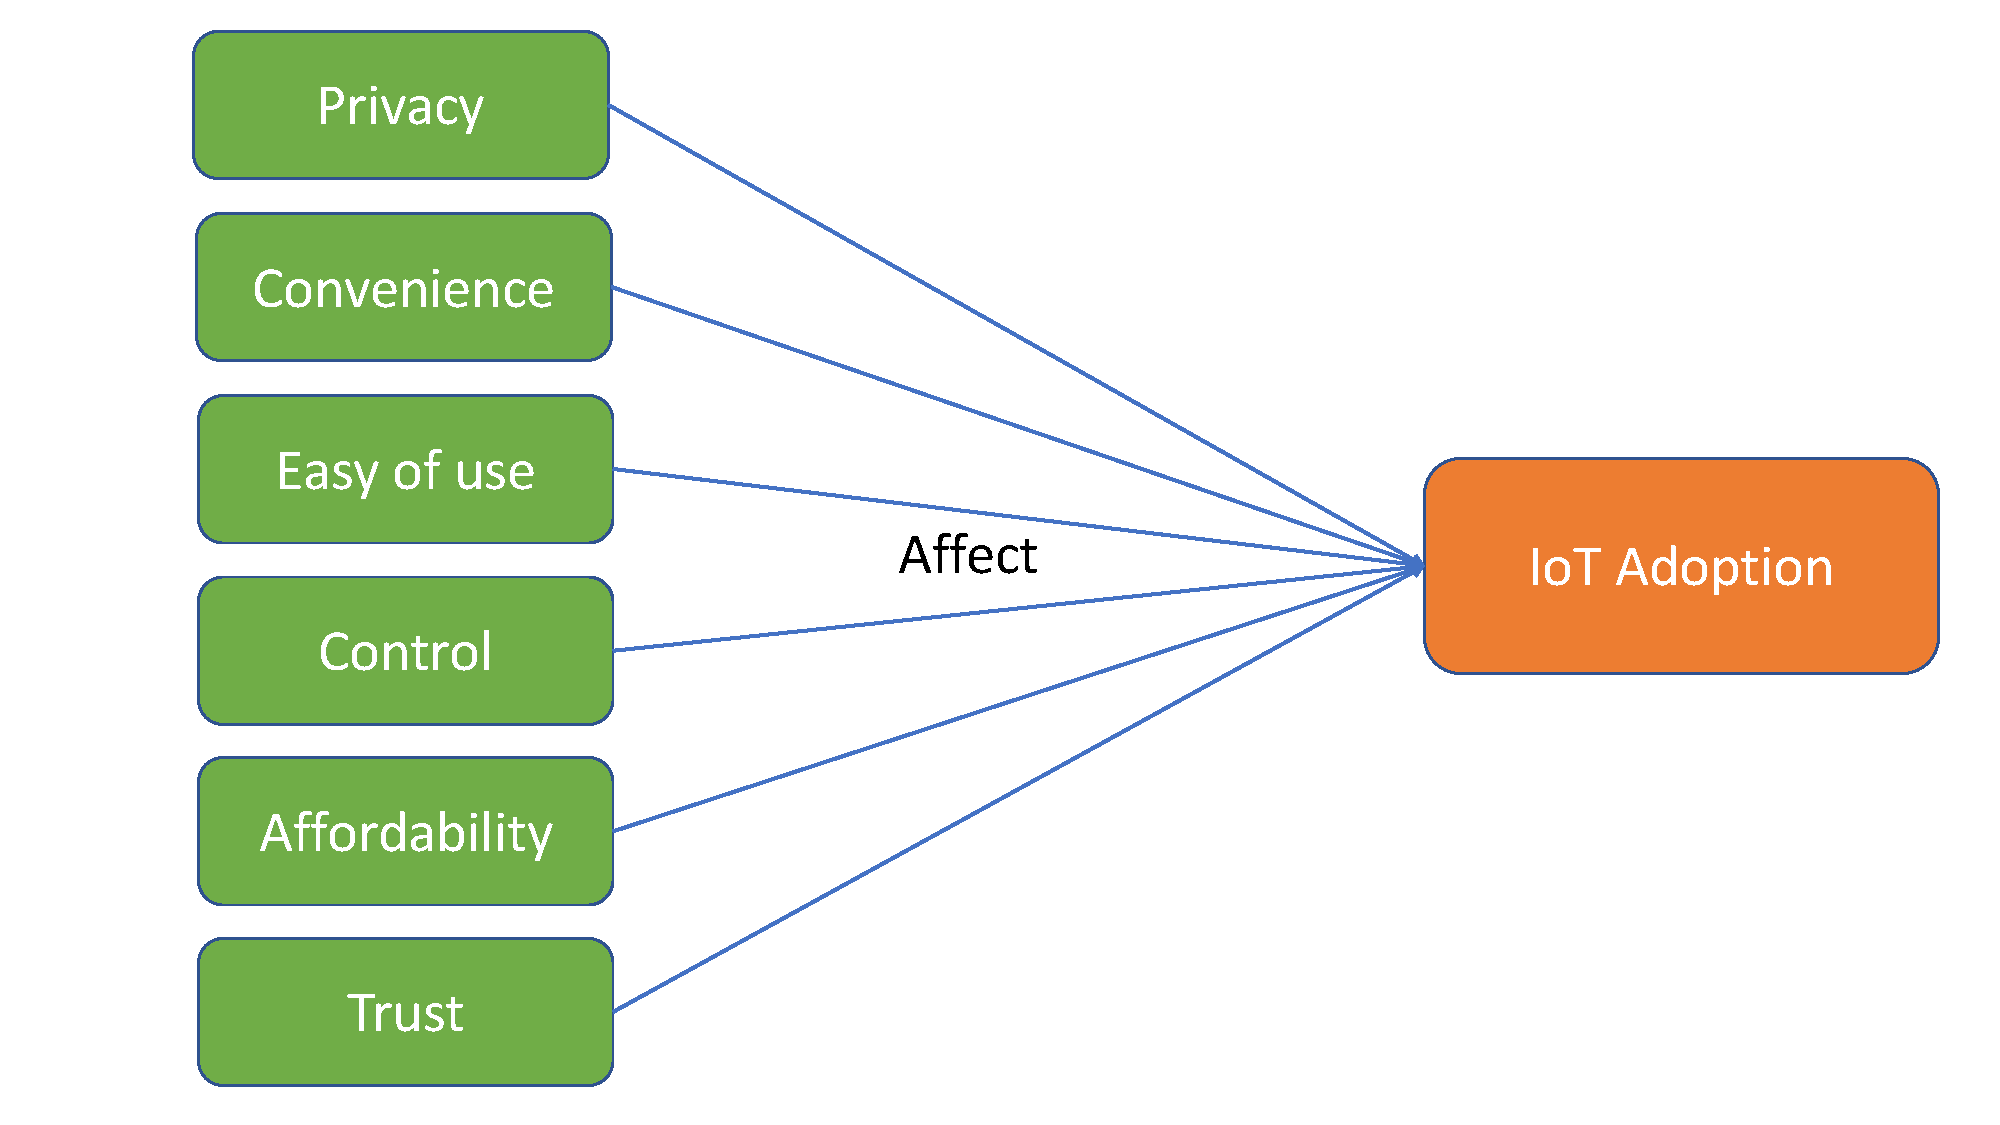
\includegraphics[width=0.8\textwidth]{figures/pilot_study_model.pdf}
	\caption{The factors that affecting users' adoptions of IoT found in our study}
	\label{fig:pilotstudymodel}
\end{figure}

The results showed similar findings as aforementioned work~\cite{gao2014unified, al2016modeling}. However, in our study, we noticed an interesting phenomenon that no literature has mentioned -- once trust with the manufacturers is established, it can propagate from the manufacturers to a third-party, which users are not aware of or even know about in the first place. We define this phenomenon as \textbf{Trust Chain}. An example of Trust Chain from our interview is:

\textit{I: ``Would you be alright if the manufacturer of those products collect your data and share with other organizations and provide more specific recommendation to you? Will you be OK with that?''}

\textit{P: ``I think I can be OK with that. Because the data this company collected are most time just shared or transferred to other companies who can analyze these data and get some information from these data.''}

\textit{I: ``Any company or any organization?''}

\textit{P: ``I think most are the manufacturers that I trust.''}

\textit{I: ``So you are OK with them to share your data?''}

\textit{P: ``Yes, I trust them.''}

As shown in Figure~\ref{fig:trustchain}, Trust Chain is established mostly because of the trust from the users to the manufacturers (i.e. the brand of the devices), and can arguably be categorized as an emotional behavior because users would not have a clear sight at the benefits and risks when they choose to trust the third parties that manufacturers choose to shared their data with. Such benefits and risks have been defined as abstract benefits and risk. One of our current undergoing research has shown that, in IoT domain, users are more likely to perceive concrete benefits and abstract risks, resulting this emotional behavior phenomenon. Such behavior could bring harm to their privacy and security. To be more rational, we suggest users to investigate the third parties that will handle their personal data. Thus, we suggest the manufacturer/designers of the IoT privacy to provide users transparency and control on what third parties they will share users' data with to reduce the risks of insecure Trust Chain sharing behavior.

\begin{figure}
	\centering
	
\includegraphics[width=0.75\columnwidth]{figures/trustchain.pdf}
	\caption{Trust Chain}
	\label{fig:trustchain}
\end{figure}

Knowing all these factors that affect users' decision on adopting IoT device will help us develop the scales for evaluating our designed privacy-setting interfaces in our proposed work (Chapter~\ref{chapter:evaluation}). Based on the insights gained from this study, we encourage the designers of IoT privacy-setting interfaces to face the difficult challenge of maximizing the usability and the privacy control of the user interface while minimizing the privacy threats to the users, making IoT more acceptable.

\section{Summary}
In this chapter, I have noted the following points: 1) IoT have grown in use rapidly with the advancing of RFID and other wireless sensor technologies. 2) IoT have brought convenience and enjoyment to our daily lives. 3) Privacy concern is an important factor that affect users' decisions when adopting IoT. 4) The acceptance of IoT is still not systematically examined.


In the next chapter, we discuss the reason that cause the privacy issues in IoT, how effective existing privacy control schemes are, and the work that aims to help users protect their privacy more effectively.



















\chapter{Privacy setting technologies in IoT}\label{chapter:Relatedwork2}
In chapter~\ref{chapter:Relatedwork1}, we discuss the development of IoT and its acceptance model. As IoT systems gain popularity and bring privacy issues at the same time, it is urgent to study the cause of these privacy issues. By doing this, we can improve our design of IoT applications to protect IoT users' privacy, and make IoT more acceptable.

\section{Privacy Preference}
Researchers have attempted to examine users' privacy preferences in different areas, such as Social Networks and mobile applications. Research has shown people differ extensively in their privacy settings~\cite{olson2005study}, but can be clustered into groups~\cite{anthony2007privacy,knijnenburg2013dimensionality}. In~\cite{wisniewski2014profiling, knijnenburg2017privacy}, Facebook users are found to belong to one of 6 types of privacy profiles which range from Privacy Maximizers to Minimalists. In the health/fitness domain, emerging sensors and mobile applications allow people to easily capture fine-grained personal data related to long term fitness goals. Brar and Kay discover that users' preferences change for every fitness/heath index. Weight was found the be the most important index~\cite{brar2004privacy}. 

At the same time, users are found to have difficulties managing their privacy settings with current privacy-setting schemes. Liu et al. use an online survey (N=200) to investigate the difference between the desired privacy settings and the actual privacy settings of Facebook users. Their results show that 63\% of the privacy settings for photo sharing did not match the users' desired settings. In~\cite{madejski2012study}, Madejski et al. conduct user studies to find the difference between Facebook users’ sharing intentions and their actual privacy settings. Their results show that there is at least one violation in the privacy settings for each of the 65 participants.

The reasons for the failure of existing privacy-setting schemes are diverse. One reason for this is that the increasing number of privacy rules make manual privacy configuration excessively challenging for normal users~\cite{furnell2015managing}. Knijnenburg et al. discover that people's information disclosure behaviors vary along multiple dimensions~\cite{knijnenburg2013dimensionality}. People can be classified along these dimensions into groups with different ``disclosure styles". This result suggests that we could classify users into their respective privacy groups and adapt their privacy practices to the disclosure style of this group to satisfy different types of information and users. However, on the other hand, the more privacy policies would lead to more decision-making and more burden for users. Note that in the IoT environment, the number for different IoT devices could be vast, which could potentially make choosing adequate privacy settings a very challenging task that is likely to result in information and choice overload~\cite{williams2016perfect}. Therefore, in this thesis, we will use a data-driven approach (machine learning techniques) to discover suitable smart privacy profiles, which are generated from the results of both statistical analysis and machine learning techniques, for users with different ``disclosure styles".

\section{Privacy in IoT}
IoT systems are capable of providing a highly personalized services to their users~\cite{vallee2016personalization, etzion2014personalization, hemant2015internet}. Henka et al.~\cite{henka2016personalizing} propose an approach to personalize services in household IoT using the Global Public Inclusive Infrastructure's~\cite{vanderheiden2011creating} preference set to describe an individual's needs and preferences, and then adapting a smart environment accordingly. Russell et al.~\cite{russell2015personalization} use unobtrusive sensors and a micro-controller to realize human detection to provide personalization in a household IoT environment.

Researchers have shown that privacy plays a limiting role in users' adoption of personalized services~\cite{teltzrow_2004}. For example, Awad and Krishnan~\cite{awad_2006} show that privacy concerns inhibit users' use of personalized services, and Sutanto et al.~\cite{sutanto_2013} demonstrated that privacy concerns can prevent people from using a potentially beneficial personalized application. Kobsa et al.~\cite{kobsa_2016} demonstrate that the personalization provider is an important determinant of users' privacy concerns.

Moreover, research has shown  users' willingness to provide personal information to personalized services depends on both the risks and benefits of disclosure~\cite{phelps_2000,ho_2006,hui_2006}, and researchers therefore claim that both the benefits and the risks meet a certain threshold~\cite{treiblmaier_2007}, or that they should be in balance~\cite{chellappa_2005}.

The argument that using user-generated data for personalization can result in privacy concerns has also been made in IoT environments~\cite{worthy_trust_2016, gao2014unified, al2016modeling}. One of the first examples in this regard was the work by Sheng et al.~\cite{sheng_experimental_2008}, who showed that users of ``u-commerce'' services (IoT-driven mobile shopping) felt less inclined to use personalized (rather than non-personalized) u-commerce services, unless the benefits were overwhelming (i.e., providing help in an emergency).

In response, researchers have proposed frameworks with guidelines for evaluating the security and privacy of consumer IoT applications, devices, and platforms~\cite{perera_privacy-by-design_2016, loi_systematically_2017}. Most of these guidelines are focused on minimizing data acquisition, storage, and collection sources. Along these guidelines, several researchers have proposed architectures that restrict unwanted access to users' data by IoT devices. For example, Davies et al. propose ``privacy mediators'' to the data distribution pipeline that would be responsible for data redaction and enforcement of privacy policies even before the data is released from the user's direct control~\cite{davies_privacy_2016}. Likewise, Jayraman et al.'s privacy preserving architecture aggregates requested data to preserve user privacy~\cite{jayaraman_privacy_2017}.

Other research has considered IoT privacy from the end-user perspective~\cite{feth_user-centered_2017}, both when it comes to research (e.g., Ur et al. investigated how privacy perceptions differ among teens and their parents in smart security systems installed in homes~\cite{ur_intruders_2014}) and design (e.g., Williams et al. highlight the importance of designing interfaces to manage privacy such that they are usable to the end users of IoT devices~\cite{williams2016perfect}, and Feth et al. investigated the creation of understandable and usable controls~\cite{feth_user-centered_2017}). We followed this approach and developed a novel data-driven approach to developing usable and efficient privacy-setting interfaces for several different IoT contexts.

\section{Existing Privacy Setting Models}
Previous studies in smartphone privacy have shown that the current smartphone privacy interfaces lack the potential to provide the necessary user privacy information or control for both Android and iOS systems~\cite{lin2014modeling}. Several solutions have been proposed to improve mobile privacy protection and offer users more privacy control~\cite{felt2012android, beresford2011mockdroid}. These lead into rapid improvement of privacy management of current mobile systems, providing more control on the user's privacy settings.

Android system mainly use Ask On Install (AOI) and Ask On First Use (AOFU) models for privacy settings~\cite{tsai2017turtle, wijesekera2017feasibility}. In the AOI model, the smartphone permissions are asked in bulk before installing a new app. The user's option is only to allow or deny all, which clearly gives less privacy control. Also, only few users would read or pay attention to the privacy settings when installing the app, and even fewer users can understand their meaning~\cite{felt2012android,kelley2012conundrum}. Several third-party apps have been developed to cope with this problem, such as Turtleguard~\cite{tsai2017turtle} and Mockdroid~\cite{beresford2011mockdroid}. %, Advanced Permission Manager\cite{},Xprivacy\cite{}, Permission Master~\cite{}, DonkeyGuard\cite{}, AppOps\cite{}. 
In the AOFU model~\cite{tsai2017turtle}, permissions are only asked during the first use of an app or when some function of the app is demanding a specific permission of the smartphone. In this case, the user will trade off his privacy (data sharing) and the functionality of the app. Users can also revisit and review permissions in their phone privacy settings for each app. This model makes users more informed and gives them more control compared to AOI~\cite{fu2014field}.

A few privacy management solutions were developed to simplify the task of controlling personal data for smartphone users. For instance, ipShield~\cite{chakraborty2014ipshield} is a context-aware privacy framework for mobile systems that provides users with great control of their data and inference risks. My Data Store \cite{ref:vescovi} offers a set of tools to manage, control and exploit personal data by enhancing an individual’s awareness of the value of their data. Similarly, Databox~\cite{ref:chaudhry} enables individuals to coordinate the collection of their personal data, and make those data available for specific purposes. However, these data managers do not include user privacy profiling and recommendation in the complex IoT environment. Privacy can also be protected by providing different anonymity levels of data that are given to third parties. However, it might not be possible to implement the most effective privacy standards such as data obfuscation due to numerous trade-offs and restrictions, especially in the health care and fitness domain.

In the smartphone domain, privacy nudging is an effective scheme to increase users' awareness~\cite{almuhimedi2015your}. Privacy nudging allows users to be informed about both their privacy settings and how third party applications access their data~\cite{liu2016follow,fu2014field}. In a study by Liu et al., 78.7\%~\cite{liu2016follow} of the nudges were adopted by smartphone users. However, such nudges are problematic for IoT, because IoT devices are supposed to operate in the background. Moreover, as the penetration of IoT devices in our homes continues to increase, nudging would become a constant noise which users would soon start to ignore, like software EULAs~\cite{good2005spyware} or privacy policies~\cite{jensen2004privacy}. In addition, privacy nudges lack the personalization and provide only a general recommendation.

%Another approach which is more user-centric is the user-tailored privacy~\cite{knijnenburg2017privacy}. It models users’ privacy concerns and provides them with adaptive privacy decision support. This model can be seen as personalized ``smart nudges'' where the recommendation is aligned with the user's privacy preference. User-tailored privacy aids users in making privacy decisions by providing them the right amount of both the privacy-related information associated to them and the useful privacy control that do not overwhelm or mislead them. However, in practice it is hard to implement general privacy model as the idea is too broad and abstract especially in the diversity of privacy perception of users. 

%\textit{khealth} is an IoT framework based on a personalized digital health care information system that protects users from third parties' advertisements~\cite{sharma2018toward}. Pejovic and Musolesi~\cite{Pejovic2014} presented the design and implementation of an efficient online learner that can serve as a basis for recognizing opportune moments for interruption. The design of the library is based on an in-depth study of human interruptibility. Comparatively, our work tries to find the most suitable privacy-setting profile for each user based on their privacy preference on different household IoT scenarios.

\section{Privacy-Setting Interfaces}
Beyond prompts, one can regulate privacy with global settings. The most basic privacy-setting interface is the traditional ``access control matrix'', which allows users to indicate which entity gets to access what type of information~\cite{sandhu1994access}. This approach can be further simplified by grouping recipients into relevant semantic categories, such as Google+'s \emph{circles}~\cite{watson12}. Taking a step further, Raber et al.~\cite{197908} proposed \emph{Privacy Wedges} to manipulate privacy settings. Privacy Wedges allow users to make privacy decisions using a combination of semantic categorization (the various wedges) and inter-personal distance (the position of a person on the wedge). Users can decide who gets to see various posts or personal information by ``coloring'' parts of each wedge. 

Privacy wedges have been tested on limited numbers of friends, and in the case of household IoT they are likely to be insufficient, due to the complexity of the decision space. To wit, IoT privacy decisions involve a large selection of devices, each with various sensors that collect data for a range of different purposes. This makes it complicated to design an interface that covers every possible setting~\cite{williams2016perfect}. A wedge-based interface will arguably not be able to succinctly represent such complexity, and therefore either be impossible, or still lead to a significant amount of information and choice overload. 

We used a data-driven approach to solve this problem: statistical analysis informs the construction of a layered settings interface, while machine learning-based privacy prediction helps us find smart privacy profiles.

\section{Privacy Prediction}
Several researchers have proposed privacy prediction as a solution to the privacy settings complexity problem---an approach known as ``user-tailored privacy'' (UTP)~\cite{knijnenburg2017}. Systems that implement UTP first predict users' privacy preferences and behaviors based on their known characteristics. They then use these predictions to provide automatic default settings or suggestions in line with users' disclosure profiles, to educate users about privacy features they are unaware of, to tailor the privacy-setting user interfaces to make it easier for users to engage with their preferred privacy management tools, or to selectively restrict the types of personalization a system is allowed engage in.

Most existing work in line with this approach has focused on providing automatic default settings. For example, Sadeh et al.~\cite{sadeh2009understanding} used a k-nearest neighbor algorithm and a random forest algorithm to predict users' privacy preferences in a location-sharing system, based on the type of recipient and the time and location of the request. They demonstrated that users had difficulties setting their privacy preferences, and that the applied machine learning techniques can help users to choose more accurate disclosure preferences. Similarly, Pallapa et al.~\cite{pallapa2014adaptive} present a system which can determine the required privacy level in new situations based on the history of interaction between users. Their system can efficiently deal with the rise of privacy concerns and help users in a pervasive system full of dynamic interactions.

Dong et al.~\cite{dong2016ppm} use a binary classification algorithms to give users personalized advice regarding their privacy decision-making practices on online social networks. They found that J48 decision trees provided the best results. Li and et al.~\cite{li2017cross} similarly use J48 to demonstrate that taking the user's cultural background into account when making privacy predictions improves the prediction accuracy. Our data stems from a culturally homogeneous population (U.S. Mechanical Turk workers), so cultural variables are outside the scope of our study. We do however follow these previous works in using J48 decision trees in our prediction approach.

We further extend this approach using \emph{clustering} to find several smart default policies (``profiles''). This is in line with Fang et al.~\cite{fang2010privacy}, who present an active learning algorithm that comes up with privacy profiles for users in real time. Since our approach is based on an existing dataset, our algorithm does not classify users in real time, but instead creates a static set of profiles `offline', from which users can subsequently choose. This avoids cold start problems, and does not rely on the availability of continuous real-time behaviors. This is beneficial for household IoT privacy settings, because users often specify their settings in these systems in a ``single shot'', leaving the settings interface alone afterwards.

Ravichandran et al.~\cite{ravichandran2009capturing} employ an approach similar to ours, using $k$-means clustering on users' contextualized location sharing decisions to come up with several default policies. They showed that a small number of policies could accurately reflect a large part of the location sharing preferences. 

In this proposal, we extend this \emph{clustering} approach to find the best profiles based on various novel clustering approaches, and take the additional step of designing user interfaces that incorporate the best solutions for different IoT contexts.

\section{Summary}
In this chapter, we have noted following points: 1) Existing research has shown that people are extensively different in their privacy settings, but can be grouped. 2) People are bad at managing privacy settings using currently privacy setting schemes. 3) Privacy prediction can be used by utilizing machine learning algorithms to help design a new privacy-setting interface to simplify the task of managing privacy setting for users. 

In the next chapter, we will present how we design for privacy in the general/public IoT context using a data-driven approach, the contributions and the limitations of our work.
	% !TeX root = proposal.tex
\chapter{Recommending Privacy Settings for Generalized/Public IoT}\label{chapter:generalIoT}

In chapter~\ref{chapter:acceptability}, we have discussed what are the key factors affecting users to adopt IoT systems/devices, the privacy risks caused by inappropriate privacy disclosure and the difficulties that people have when manually configuring their privacy-setting for their IoT systems/devices. To alleviate similar burden of doing this in OSN/mobile areas, researchers have applied machine learning techniques to predict people’s location-privacy preferences, thereby automatically configuring their location-privacy settings. 
%But none similar research has been done in IoT domain yet. 
Therefore, we speculate that machine learning algorithm based user clustering can also be used to recommend privacy-setting for IoT users.

In this chapter, we demonstrate our work completed in exploring recommending privacy settings for general IoT, including the dataset that we use, our methodology, the inspection of users' behaviors using statistical analyses, prediction of users' behaviors using machine learning techniques, and the privacy-setting prototypes that we create based on both statistical and machine learning results.

In this chapter the following questions will be answered:
\begin{itemize}
	\item Q1: What are the key parameters affecting the users' privacy decisions in a general IoT scenario?
	\item Q2: Can you cluster users of general IoT and provide them effective and accurate smart default/profiles of privacy-settings using machine learning techniques?
\end{itemize}

As we have already discussed, there is similarity in people’s privacy preferences. Therefore,
neighbourhood-based recommendations may be as accurate as model-based recommendations.
Furthermore, neighbourhood-based recommendations are made from crowdsourcing sources,
which means that their performance may be better than that of model-based recommenders when
the data of individual users are insufficient.

\section{Dataset and design}
As we have discussed in Chapter \ref{chapter:intro}, the development of usable privacy interfaces commonly relies on user studies with existing systems. Since the Intel control framework has yet to be implemented~\cite{chow2015hci}, this method is not possible. We therefore we leveraged data collected by Lee and Kobsa~\cite{lee2016understanding}, which asked 200 participants about their intention to allow or reject the IoT features presented in 14 randomized scenarios. They varied the scenarios in a mixed fractional factorial design along the following dimensions: `Who', `What', `Where', `Reason', and `Persistence' (See Table~\ref{tab:parameter}). A total of 2800 scenarios were presented to 200 participants (100 male, 99 female, 1 undisclosed) through Amazon Mechanical Turk. Four participants were aged between 18 and 20, 75 aged 20--30, 68 aged 30--40, 31 aged 40--50, 20 aged 50--60, and 2 aged $>$ 60.

For every scenario, participants were asked a total of 9 questions. Our study focuses on the \textbf{allow/reject} question: ``If you had a choice to allow/reject this, what would you choose?'', with options ``I would allow it'' and ``I would reject it''. We also used participants' answers to three attitudinal questions regarding the scenario:
\begin{itemize}
	\item \textbf{Risk:} How risky or safe is this situation? (7pt scale from ``very risky'' to ``very safe'')
	\item \textbf{Comfort:} How comfortable or uncomfortable do you feel about this situation? (7pt scale)
	\item \textbf{Appropriateness:} How appropriate do you consider this situation? (7pt scale)
\end{itemize}

\begin{table*}
	\caption{Parameters used in the experiment. Example scenarios: \\\emph{``A device of a friend records your video to detect your presence. This happens continuously, while you are at someone else's place, for your safety.''}\\\emph{``A government device reads your phone ID to detect your identity. This happens once, while you are in a public place (e.g. on the street), for health-related purposes.''}}
	\label{tab:parameter}
	\begin{tabular}{l | l}
		\hline
		\textbf{Parameter} & \textbf{Levels} 	 \\ \hline
		\multirow{7}{9.5em}{Who\\\rule{0pt}{4ex}\emph{The entity collecting the data}}		& 1. Unknown \\
		& 2. Colleague							 \\
		& 3. Friend								 \\
		& 4. Own device							 \\
		& 5. Business 							 \\
		& 6. Employer 							 \\
		& 7. Government							 \\ \hline
		\multirow{24}{9.5em}{What\\\rule{0pt}{4ex}\emph{The type of data collected and (optionally) the knowledge extracted from this data}}	& 1. PhoneID	\\	
		& 2. PhoneID$>$identity				\\	
		& 3. Location						\\	
		& 4. Location$>$presence			\\	
		& 5. Voice							\\	
		& 6. Voice$>$gender					\\	
		& 7. Voice$>$ age 					\\	
		& 8. Voice$>$identity				\\	
		& 9. Voice$>$presence				\\	
		& 10. Voice$>$mood					\\	
		& 11. Photo							\\	
		& 12. Photo$>$gender				\\	
		& 13. Photo$>$age  \\
		& 14. Photo$>$identity	 \\
		& 15. Photo$>$presence 	 \\
		& 16. Photo$>$mood 	 \\
		& 17. Video	 \\
		& 18. Video$>$gender	 \\
		& 19. Video$>$age 		 \\
		& 20. Video$>$presence 	 \\
		& 21. Video$>$mood 	 \\
		& 22. Video$>$looking at	 \\
		& 23. Gaze	 \\
		& 24. Gaze$>$looking at	 \\ \hline
		\multirow{4}{9.5em}{Where\\\rule{0pt}{4ex}\emph{The location of the data collection}}	& 1. Your place		\\
		& 2. Someone else's place		\\				
		& 3. Semi-public place (e.g. restaurant) \\
		& 4. Public space (e.g. street) \\ \hline
		\multirow{6}{9.5em}{Reason\\\rule{0pt}{4ex}\emph{The reason for collecting this data}} & 1. Safety	\\
		& 2. Commercial						\\
		& 3. Social-related	\\
		& 4. Convenience \\
		& 5. Health-related \\
		& 6. None \\ \hline
		\multirow{2}{9.5em}{Persistence} & 1. Once \\
		& 2. Continuously \\ 
		\emph{Whether data is collected once or continuously} & \\ \hline
	\end{tabular}
\end{table*}

We use this dataset in two phases. In our first phase, we develop a ``layered'' settings interface, where users make a decision on a less granular level (e.g., whether a certain recipient is allowed to collect their personal information or not), and only move to a more granular decision (e.g., what types of information this recipient is allowed to collect) when they desire more detailed control. This reduces the complexity of the decisions users have to make, without reducing the amount of control available to them. We use statistical analysis of the Lee and Kobsa dataset to decide which aspect should be presented at the highest layer of our IoT privacy-setting interface, and which aspects are relegated to subsequently lower layers.

In our second phase, we develop a ``smart'' default setting, which preempts the need for many users to manually change their settings~\cite{smith2013choice}. However, since people differ extensively in their privacy preferences~\cite{olson2005study}, it is not possible to achieve an optimal default that is the same for everyone. Instead, different people may require different settings. Outside the field of IoT, researchers have been able to establish distinct clusters or ``profiles'' based on user behavioral data~\cite{knijnenburg2013dimensionality, olson2005study, wisniewski2017making}. We perform machine learning analysis on this dataset to create a similar set of ``smart profiles'' for our general IoT privacy-setting interface.

\section{Statistical Analysis}\label{sec:sa1}

%
%In this section we analyze how users' behavioral intentions to allow or reject the information collection described in the scenario are influenced by the scenario parameters. In line with classic attitude-behavior models~\cite{ajzen1977attitude}, we also investigate whether users' attitudes regarding the scenario---their judgment of risk, comfort, and appropriateness---mediate these effects. This mediation analysis~\cite{baron1986moderator} involves the following test:
%\begin{itemize}
%\item \textbf{Test 1:} The effect of the scenario parameters (who, what, where, reason, persistence) on participants' attitudes (risk, comfort, appropriateness).
%\item \textbf{Test 2:} The effect of participants' attitudes on their behavioral intentions (the allow/reject decision).
%\item \textbf{Test 3:}  The effect of the parameters on behavioral intentions, controlling for attitudes.
%\end{itemize}
%
%If tests 1 and 2 are significant, and test 3 reveals a substantial reduction in conditional direct effect (compared to the marginal effect), then we can say that the effects of the scenario parameters on participants' behavioral intention are mediated by their attitudes. Moreover, if the conditional direct effect is (close to) zero, then the effects are fully (rather than partially) mediated.
%
%\subsection{Scenario Parameters and Attitude}\label{subsec:attitude}
%\subsubsection{ANOVA Test of Main Effects}
%To understand the effect of the scenario parameters on participants' attitudes, we created a separate \textit{linear mixed effects regression} (\textit{lmer}) model with a random intercept (to account for repeated measures on the same participant) for each dependent variable (risk, comfort, appropriateness), using the scenario parameters as independent variables. We employed a forward stepwise procedure, adding the strongest remaining parameter into the model at each step and comparing it against the previous model. Table~\ref{tab:anovaEffect} shows that all parameters except \textbf{where} have a significant effect on each of the attitudes.
%
%\subsubsection{Post-hoc Comparisons}
%We also conducted Tukey post hoc analyses to better understand how the various values of each parameter influenced the attitudes. \textbf{Where} was excluded from these analyses, as it did not have an overall significant effect. Some key findings of these post hoc analyses are:
%
%\begin{table}
%\centering
%\caption{Effect of scenario on attitudes. Each model builds upon and is tested against the previous.}
%\label{tab:anovaEffect}
%\begin{tabular}{ l | r | r | r}
%\hline
%Model &	$\chi^2$ &	$df$ & $p$-value \\ \hline
%$risk\sim(1|sid)$ &				 &			 &						\\
%+who &				315.37 &	6 &			$<$ .0001 		\\
%+what &			67.74 &		23 &		$<$ .0001 		\\
%+reason & 			15.65 &		5 &		.0079 			\\
%+persistence &		9.95 &		1 &		.0016 			\\
%+where	&			7.47 &		3 &		.0586 			\\
%+who:what &		166.47 &	138 &	.0050			\\
%\hline
%Model &	$\chi^2$ &	$df$ & $p$-value \\ \hline
%$comfort\sim(1|sid)$ & 			 &			&	 					\\
%+who &				334.06 &	6 &			$<$ .0001 		\\
%+what &			83.24 &		23 &		$<$ .0001 		\\
%+reason &			18.68 &		5 &			.0022 		\\
%+persistence &		14.73 &		1 &			.0001 		\\
%+where &			3.25 &		3 &			.3544 		\\
%+who:what &		195.07 &	138 &		.0001			\\
%\hline
%Model &	$\chi^2$ &	$df$ & $p$-value \\ \hline
%$appropriateness\sim(1|sid)$ &	 &		 &						\\
%+who &				315.77 &	6 &			$<$ .0001 		\\
%+what &			72.87 &		23 &		$<$ .0001 		\\
%+reason &			23.27 &		5 &			.0003 		\\
%+persistence &		8.97 &		1 &			.0027 		\\
%+where &			5.46 &		3 &			.1411 		\\
%+who:what &		214.61 &	138 &		$<$ .0001			\\
%\hline
%\end{tabular}
%\end{table}
%
%\textbf{Who:} Participants perceive more \emph{risk} when the recipient of the information is `unknown' than for any other recipient ($d$ range = [0.640, 1.450] and all $p$s~$<$~.001, except for `government': $d=0.286$, $p < .05$). `Government' is the next most risky recipient ($d$ range = [0.440, 1.190], all $p$s~$<$~.001). Participants consider their `own device' the least risky ($d$ range = [0.510, 1.450], all $p$s~$<$~.001). Similar patterns were found for \emph{comfort} and \emph{appropriateness}.
%
%\textbf{Reason:} Participants were more \emph{comfortable} disclosing information for the purpose of `safety' than for any other reason except `health' ($d$ range = [0.230, 0.355], all $p$s~$<$~.05). They also believe that disclosing information for the purpose of `health' or `safety' is more \emph{appropriate} than for `social' or `commercial' purposes ($d$ range = [0.270, 0.310], all $p$s~$<$~.05).
%
%\textbf{Persistence:} Participants were more \emph{comfortable}, found it more \emph{appropriate}, and less \emph{risky} to disclose their information `once' rather than `continuously' ($d = 0.146$, $p < .01$).
%
%\textbf{What:} This parameter has a large number of values, so we decided to selectively test planned contrasts instead of post-hoc tests. We first compared different mediums (voice, photo, video) regardless of what is being inferred:
%\begin{itemize}
%\item Participants were significantly more \emph{comfortable} with `voice' than `video' ($d = 0.260$, $p = .005$), and found `voice' less \emph{risky} ($d = -0.239$, $p = .005$) and more \emph{appropriate} ($d = 0.217$, $p = .015$) than `video'.
%\item Participants were significantly more \emph{comfortable} with `voice' than `photo' ($d=0.201$, $p = .007$) and found `voice' more \emph{appropriate} than `photo' ($d = 0.157$, $p$~$=$~$.028$). There was no significant difference in terms of \emph{risk} ($p = .118$).
%\item No differences were found between `photo' and `video' in terms of \emph{risk} ($p = .24$), \emph{comfort} ($p = .35$) and \emph{appropriateness} ($p = .26$).
%\end{itemize}
%
%We also compared different inferences (e.g. age, gender, mood, identity) across mediums. The following planned contrasts were significant (all others were not):
%\begin{itemize}
%\item Participants were significantly more \emph{comfortable} ($d$~$=$~$0.363$, $p = .028$) and found it more \emph{appropriate} ($d = 0.371$, $p = .018$) to reveal their `age' rather than their `identity'.
%\item Participants were significantly more \emph{comfortable} ($d$~$=$~$0.363$, $p= .008$) and found it more \emph{appropriate} ($d = 0.308$, $p = .024$) to reveal their `presence' rather than their `identity'.
%\end{itemize}
%
%\subsubsection{Interaction effects}
%We also checked for two-way interactions between the scenario parameters. The only significant interaction effect observed was between \textbf{who} and \textbf{what}. The last line of each section in Table~\ref{tab:anovaEffect} shows the results of adding this interaction to the model. Due to space concerns, we choose not to address the post-hoc analysis of the $7 * 24 = 168$ specific combinations of who and what.
%
%\subsection{Attitude and Behavioral intention}
%To test the effects of participants' attitudes on their allow/reject decision, we ran a \emph{generalized linear mixed effects regression} (\emph{glmer}) with a random intercept and a logit link function to account for the binary dependent variable.
%We found significant effects of all the three attitudes on participants' allow/reject decision (see Table~\ref{tab:mediationANOVA}). Each 1-point increase in \textbf{risk} results in a 4.04-fold decrease in the odds that the scenario will be allowed ($p < .0001$). Each 1-point increase in \textbf{comfort} results in a 5.04-fold increase ($p < .0001$), and each 1-point increase in \textbf{appropriateness} results in a 3.47-fold increase ($p < .0001$).
%
%\subsection{Mediation Analysis}
%The bottom half of Table~\ref{tab:mediationANOVA} shows the \emph{conditional} effects of the significant parameters (who, what, reason, persistance) on participants' allow/reject decision, controlling for attitude. \textbf{Who} and \textbf{what} are no longer significant; these effects are thus fully mediated by attitude. The effects of \textbf{reason} and \textbf{persistance} are still significant, but smaller than the marginal effects (i.e., without controlling for attitude, see Table~\ref{tab:marginalANOVA})---their $\chi^2$s are reduced by 12\% and 39\%, respectively. This means that the mediation effect was substantial in all cases. The final mediation model is displayed in Figure~\ref{fig:mediationAllow}.
%
%
%\begin{table}
%\centering
%\caption{Effect of attitudes and scenario on allow/reject.}
%\label{tab:mediationANOVA}
%\begin{tabular}{ l | r | r | r | r }
%\hline
%Model & OR	&	\textbf{$\chi^2$} & $df$ & $p$-value 	\\ \hline
%$allow\sim(1 | sid)$ &	&		  &	    &				\\
%+risk &				0.25 &	1005.24  &    1 &		$<$ .0001 \\
%+comfort &			5.04 &	723.27  &     1 &		$<$ .0001 \\
%+appropriateness &	3.47 &	128.17  &	  1 & 		$<$ .0001 \\ \hline
%+who &					&	8.80	& 	  6 & 		.1851 	\\
%+what &					&	26.07 &	  	 23 &		.2976 	\\
%+reason &				&	19.33 & 	  5 & 		.0017	\\
%+persistence &			&	12.69 &	 	  1 & 		.0004 	\\
%\hline
%\end{tabular}
%\end{table}
%
%\begin{table}
%\centering
%\caption{Effect of scenario on allow/reject, \emph{not} controlling for attitudes.}
%\label{tab:marginalANOVA}
%\begin{tabular}{ l | r | r | r }
%\hline
%Model &	$\chi^2$ & $df$ & $p$-value 	\\ \hline
%$allow\sim(1 | sid)$ &		  	&	    &				\\
%+who &					221.36	& 	  6 & 		$<$ .0001 	\\
%+what &					78.55 &		  23 &		$<$ .0001 	\\
%+reason &				21.95 & 	  5 & 		  .0005		\\
%+persistence &			20.64 &		  1 & 		$<$ .0001 	\\
%\hline
%\end{tabular}
%\end{table}
%
%\begin{figure}
%\centering
%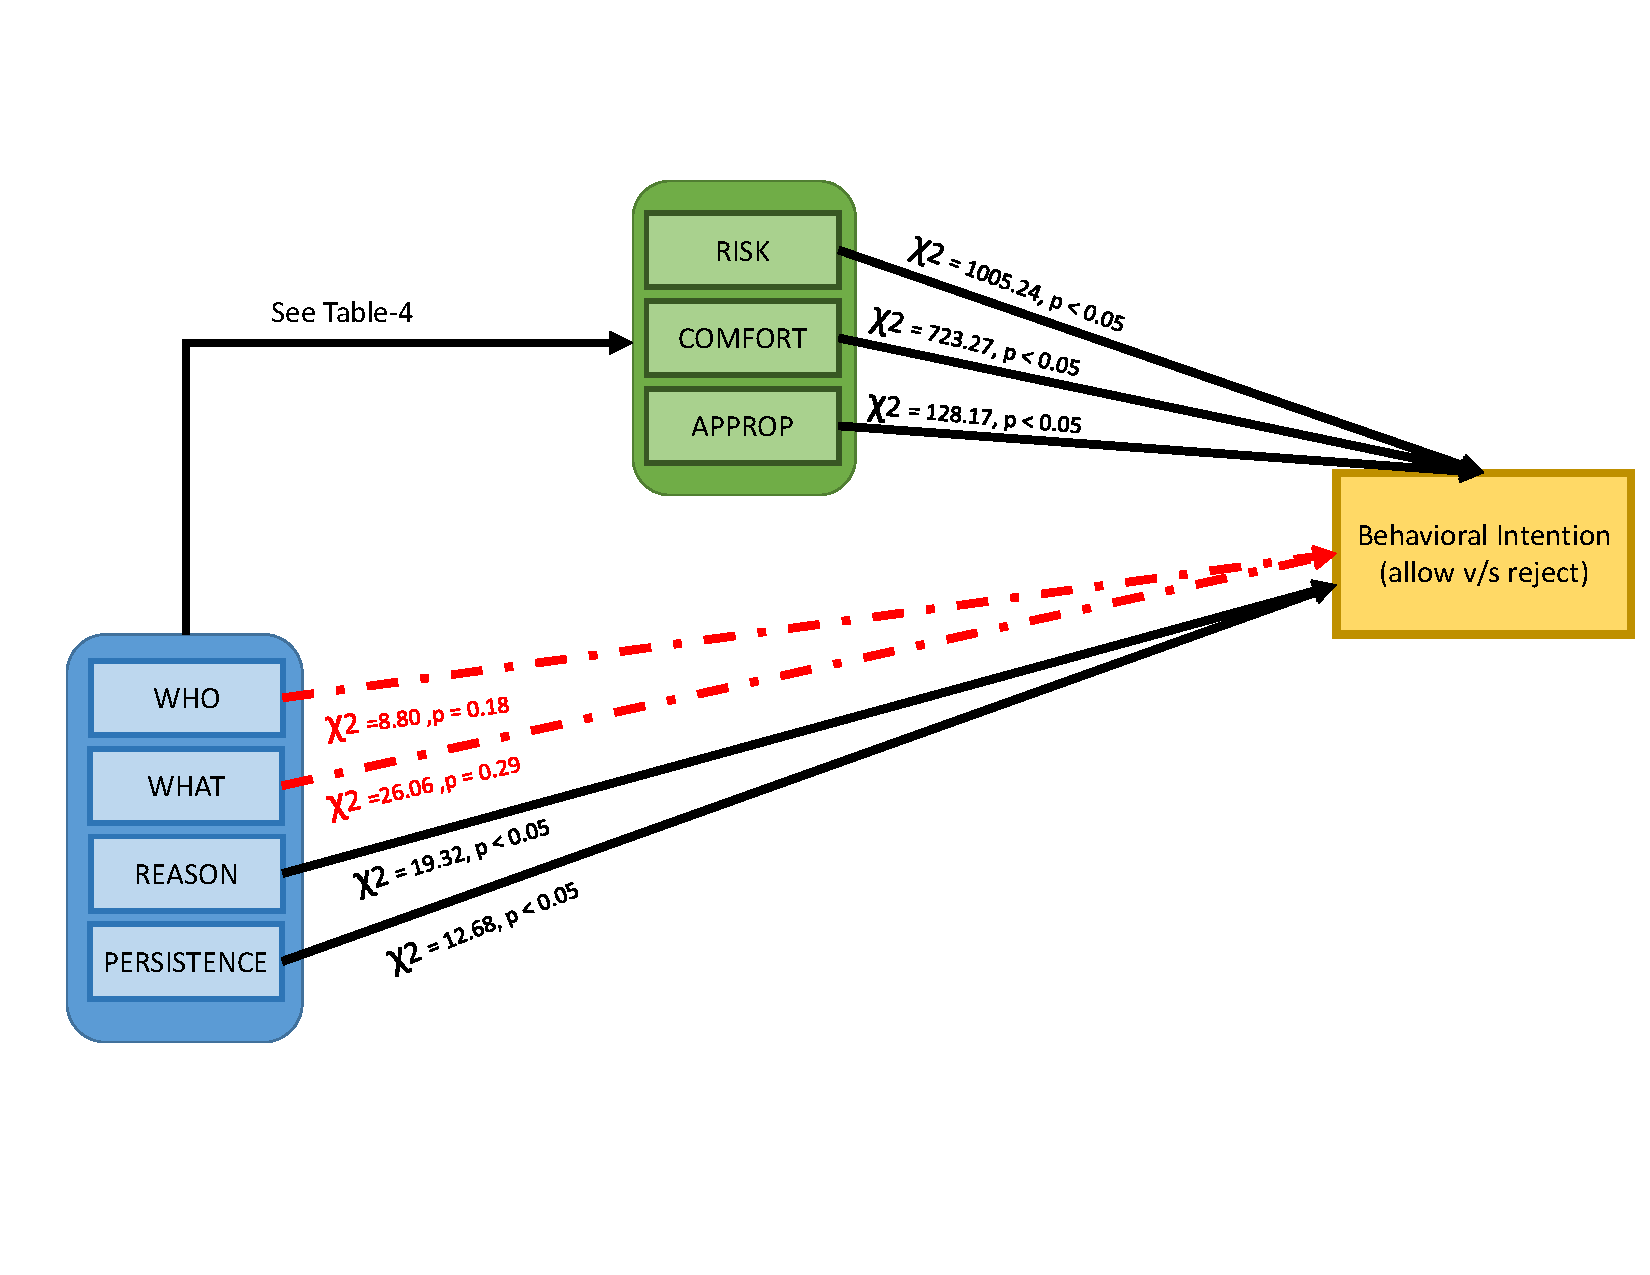
\includegraphics[width=0.45\textwidth]{figures/allow.pdf}
%\caption{Mediation model of the effect of scenario parameters on participants' intention to allow/reject the scenario, mediated by attitudinal factors}
%\label{fig:mediationAllow}
%\end{figure}

%\subsection{Discussion of Statistical Results}
We conducted a statistical analysis on this dataset to determine the effect of each scenario parameter on users' decisions to allow the presented general IoT scenario and how this effect is mediated by the user's attitudes. \footnote{The statistical analysis and the subsequent layered interface were developed by my co-author Paritosh Bahirat. These endeavors are presented in summarized form since they are not an official part of this dissertation. For more details, please refer to~\cite{bahiratiui2018}.}

Using this approach, we find that the `Who' parameter has the strongest effect on users' decision to allow the scenario, followed by the `What', the `Reason', and the 'Persistence' parameter. The `Where' parameter has no effect at all. People are generally concerned about IoT scenarios involving unknown and government devices, but less concerned about about data collected by their own devices. Mistrust of government data collection is in line with Li et al.'s finding regarding US audiences~\cite{li2017cross}.

`What' is the second most important scenario parameter, and its significant interaction with `who' suggests that some users may want to allow/reject the collection of different types of data by different types of recipients. Privacy concerns are higher for photo and video than for voice, arguably because photos and videos are more likely to reveal the identity of a person. Moreover, people are less concerned with revealing their age and presence, and most concerned with revealing their identity.

The `reason' for the data collection is the third most important scenario parameter. Health and safety are generally seen as acceptable reasons. `Persistence' is less important, although one-time collection is more acceptable than continuous collection. `Where' the data is being collected does not influence intention at all. This could be an artifact of the dataset: location is arguably less prominent when reading a scenario than it is in real life.

Finally, participants' attitudes significantly (and in some cases fully) mediated the effect of scenario parameters on behavioral intentions. This means that these attitudes may be used as a valuable source for classifying people into distinct groups. Such attitudinal clustering could capture a significant amount of the variation in participants in terms of their preferred privacy settings, especially with respect to the `who' and `what' dimensions.

Moreover, we found no significant interaction effects of parameters on decision. The only significant interaction however was between `Who' and `What' onto the attitudes. The outcome informed the design of a `layered interface', which present privacy settings with the most prominent influence first, relegating less prominent aspects to subsequently lower layers (See Figure~\ref{fig:interface1}). Users can make a decision based on a single parameter only, and choose `yes', `no', or `it depends' for each parameter value. If they choose `it depends', they move to a next layer, where the decision for that parameter value is broken down by another parameter.

The manual interface is shown in Screens 2-4 of Figure~\ref{fig:interface1}. At the top layer of this interface should be the scenario parameter that is most influential in our dataset. Our statistical results inform us that this is the \textbf{who} parameter. Screen 2 shows how users can allow/reject data collection for each of the 7 types of recipients. Users can choose ``more'', which brings them to the second-most important scenario parameter, i.e. the \textbf{what} parameter. Screen 3 of Figure~\ref{fig:interface1} shows the data type options for when the user clicks on ``more'' for ``Friends' devices''. We have conveniently grouped the options by collection medium. Users can turn the collection of various data types by their friends' devices on or off. If only some types of data are allowed, the toggle at the higher level gets a yellow color and turns to a middle option, indicating that it is not completely `on' (see ``Friends' devices'' in Screen 2).

Screen 4 of Figure~\ref{fig:interface1} shows how users can drill down even further to specify \textbf{reasons} for which collection is allowed, and the allowed \textbf{persistence} (we combined these two parameters in a single screen to reduce the ``depth'' of our interface). Since \textbf{reason} and \textbf{persistence} explain relatively little variance in behavioral intention, we expect that only a few users will go this deep into the interface for a small number of their settings. We leave out \textbf{where} altogether, because our statistical results deemed this parameter to be non-significant.

\begin{figure}
	\centering
	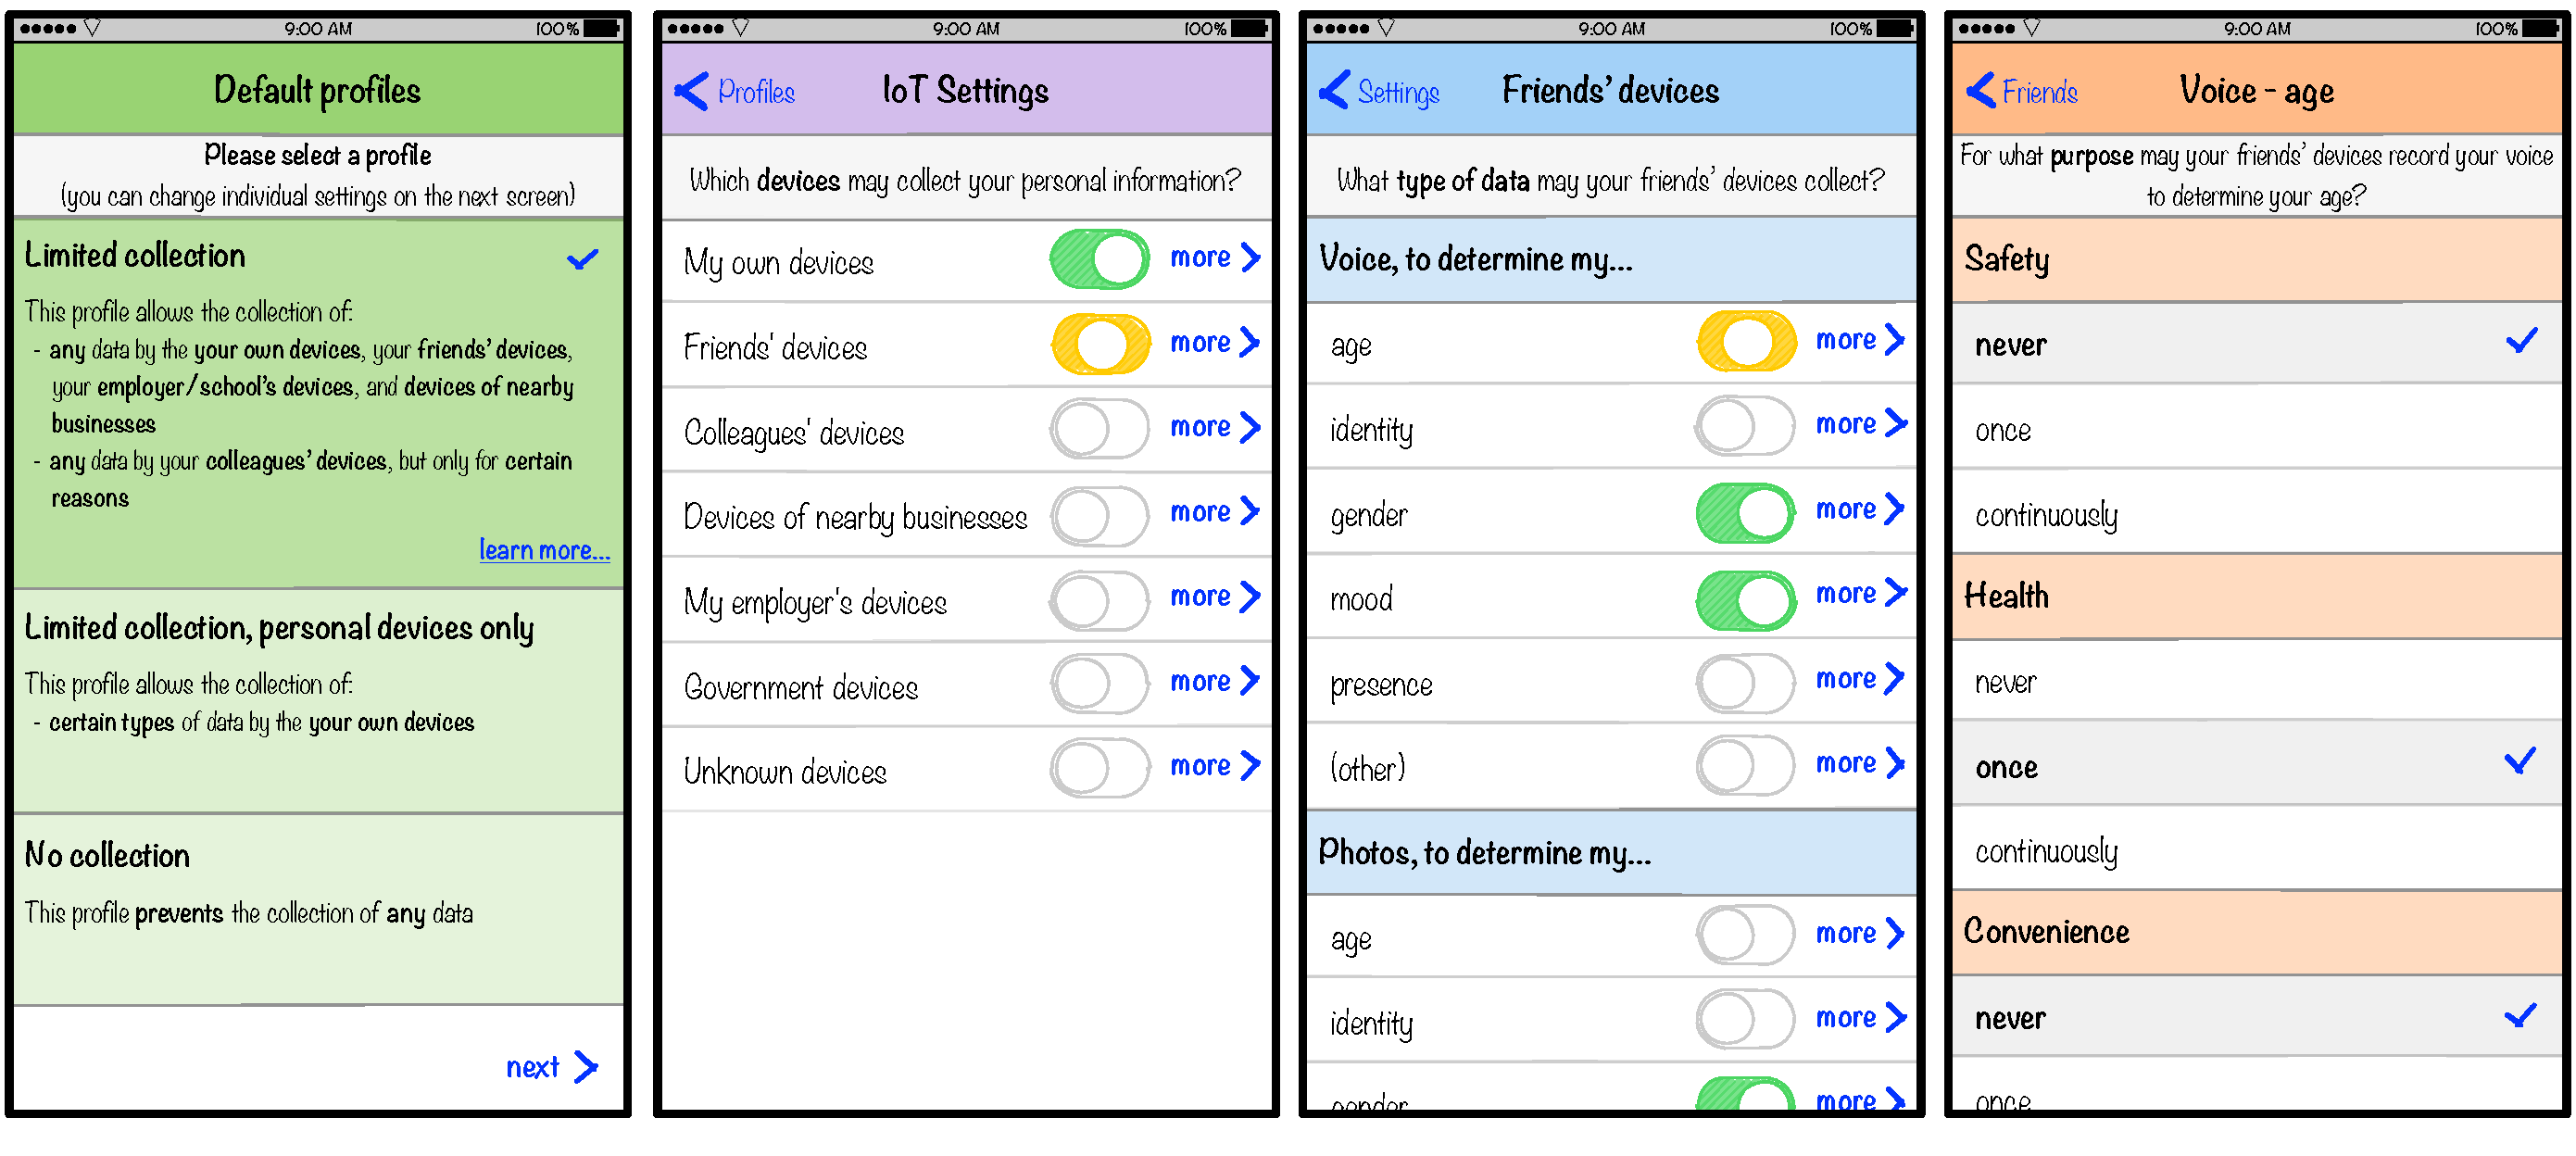
\includegraphics[width=0.8\textwidth]{figures/interface1.pdf}
	\caption{From Left, Screen 1 shows three default settings, Screen 2,3 and 4 shows layered interface}
	\label{fig:interface1}
\end{figure}

\section{Predicting users' behaviors (original work)}\label{sec:predict1}
To further simplify the task of manually setting privacy preferences, we used machine learning to predict users' decisions based on the scenario parameters. Our goal is to find suitable \emph{default settings} for an IoT privacy-setting interface. Consequently, we do not attempt to find the most accurate solution; instead we make a conscious tradeoff between parsimony and prediction accuracy. Accuracy is important to ensure that users' privacy preferences are accurately captured and/or need only few manual adjustments. Parsimony, on the other hand, prevents overfitting and promotes fairness: we noticed that more complex models tended to increase overall accuracy by predicting a few users' preferences more accurately, with no effect on other users. Parsimony also makes the associated default setting easier to understand for the user. 

Our prediction target is the participants' decision to allow or reject the data collection described in each scenario, classifying a scenario as either `yes' or `no'. The scenario parameters serve as input attributes. These are nominal variables, making decision tree algorithms such as ID3 and J48 a suitable prediction approach. Unlike ID3, J48 uses gain ratio as the root node selection metric, which is not biased towards input attributes with many values. We therefore use J48 throughout our analysis.

We discuss progressively sophisticated methods for predicting participants' decisions. After discussing naive solutions, we first present a cross-validated tree learning solution that results in a single ``smart default'' setting that is the same for everyone. Subsequently, we discuss three different procedures that create a number of ``smart profiles'' by clustering the participants and creating a separate cross-validated tree for each cluster. For each procedure, we try various numbers of clusters. Accuracies of the resulting solutions are reported in Table~\ref{tab:comp_approach}.

\subsection{Naive Prediction Methods}
We start with naive or ``information-less'' predictions. Our dataset contains 793 `yes'es and 2007 `no's. Therefore, predicting `yes' for every scenario gives us a 28.33\% prediction accuracy, while making a `no' prediction gives us an accuracy of 71.67\%. In other words, if we disallow all information collection by default, users will on average be happy with this default for 71.67\% of the settings.



\begin{table}
	\centering
	\caption{Comparison of clustering approaches}
	\label{tab:comp_approach}
	\begin{tabular}{  l |  l |  l | l}
		\hline
		Approach & clusters & Accuracy & \# of profiles \\ \hline
		\multirow{2}{6em}{Naive classification} & 1 & 28.33\% & 1  (all `yes')\\ %\cline{2-4}
		& 1 & 71.67\% & 1 (all `no') \\ \hline
		Overall & 1 & 73.10\% & 1 \\ \hline 
		\multirow{4}{6em}{Attitude-based clustering} & 2 & 75.28\% & 2 \\ %\cline{2-4}
		& 3 & 75.17\% & 3 \\ %\cline{2-4}
		& 4 & 75.60\% & 3 \\ %\cline{2-4}
		& 5 & 75.25\% & 3 \\ \hline
		%	\multirow{3}{6em}{Trait-based Clustering} & 2 & 75.57\% & 2 \\ %\cline{2-4}
		%	& 3 & 75.10\% & 2 \\ %\cline{2-4}
		%	& 4 & 75.57\% & 2 \\ %\cline{2-4}
		%	& 5 & 75.07\% & 2 \\ \hline
		\multirow{2}{6em}{Fit-based clustering} & 2 & 77.99\% & 2 \\ %\cline{2-4}
		& 3 & 81.54\% & 3 \\ \hline
		\multirow{2}{6em}{Agglomerative  clustering} & 200 & 78.13\% & 4 \\ %\cline{2-4}
		& 200 & 78.27\% & 5 \\ \hline %\cline{2-4} 
	\end{tabular}
\end{table}

\subsection{Overall Prediction}
We next create a ``smart default'' by predicting the allow/reject decision with the scenario parameters using J48 with Weka's~\cite{hall2009weka} default settings. The resulting tree is shown in Figure~\ref{fig:naive_cls}). The confusion matrix (Table~\ref{tab:confusion_matrix}) shows that this model results in overly conservative settings; only 208 `yes'es are predicted.

\begin{table}
	\centering
	\caption{Confusion matrix for the overall prediction}
	\label{tab:confusion_matrix}
	\begin{tabular}{c|c|c|c} \hline
		Observed &\multicolumn{2}{c|}{Prediction} & Total\\ \cline{2-3}
		& Yes     & No       &  \\ \hline
		Yes   & 124 (TP) & 669 (FN)  & 793   \\ \hline
		No    & 84 (FP)  & 1923 (TN) & 2007  \\ \hline
		Total & 208     & 2592     & 2800  \\ \hline
	\end{tabular}
\end{table}

Figure~\ref{fig:naive_cls} shows that this model predicts `no' for every recipient (`who') except `Own device'. For this value, the default setting depends on `what' is being collected (see Table~\ref{tab:decisions}). For some levels of `what', there is a further drill down based on `where', `persistence' and `reason'.

We can use this tree to create a ``smart default'' setting; in that case, users would on average be content with 73.10\% of these settings---a 2\% improvement over the naive ``no to everything'' default setting. 

Given that people differ substantially in their privacy preferences, it is not unsurprising that this ``one size fits all'' default setting is not very accurate. A better solution would cluster participants by their privacy preferences, and then fit a separate tree for each cluster. These trees could then be used to create ``smart profiles'' that new users may choose from. Subsequent sections discuss several ways of creating such profiles.

\begin{figure}
	\centering
	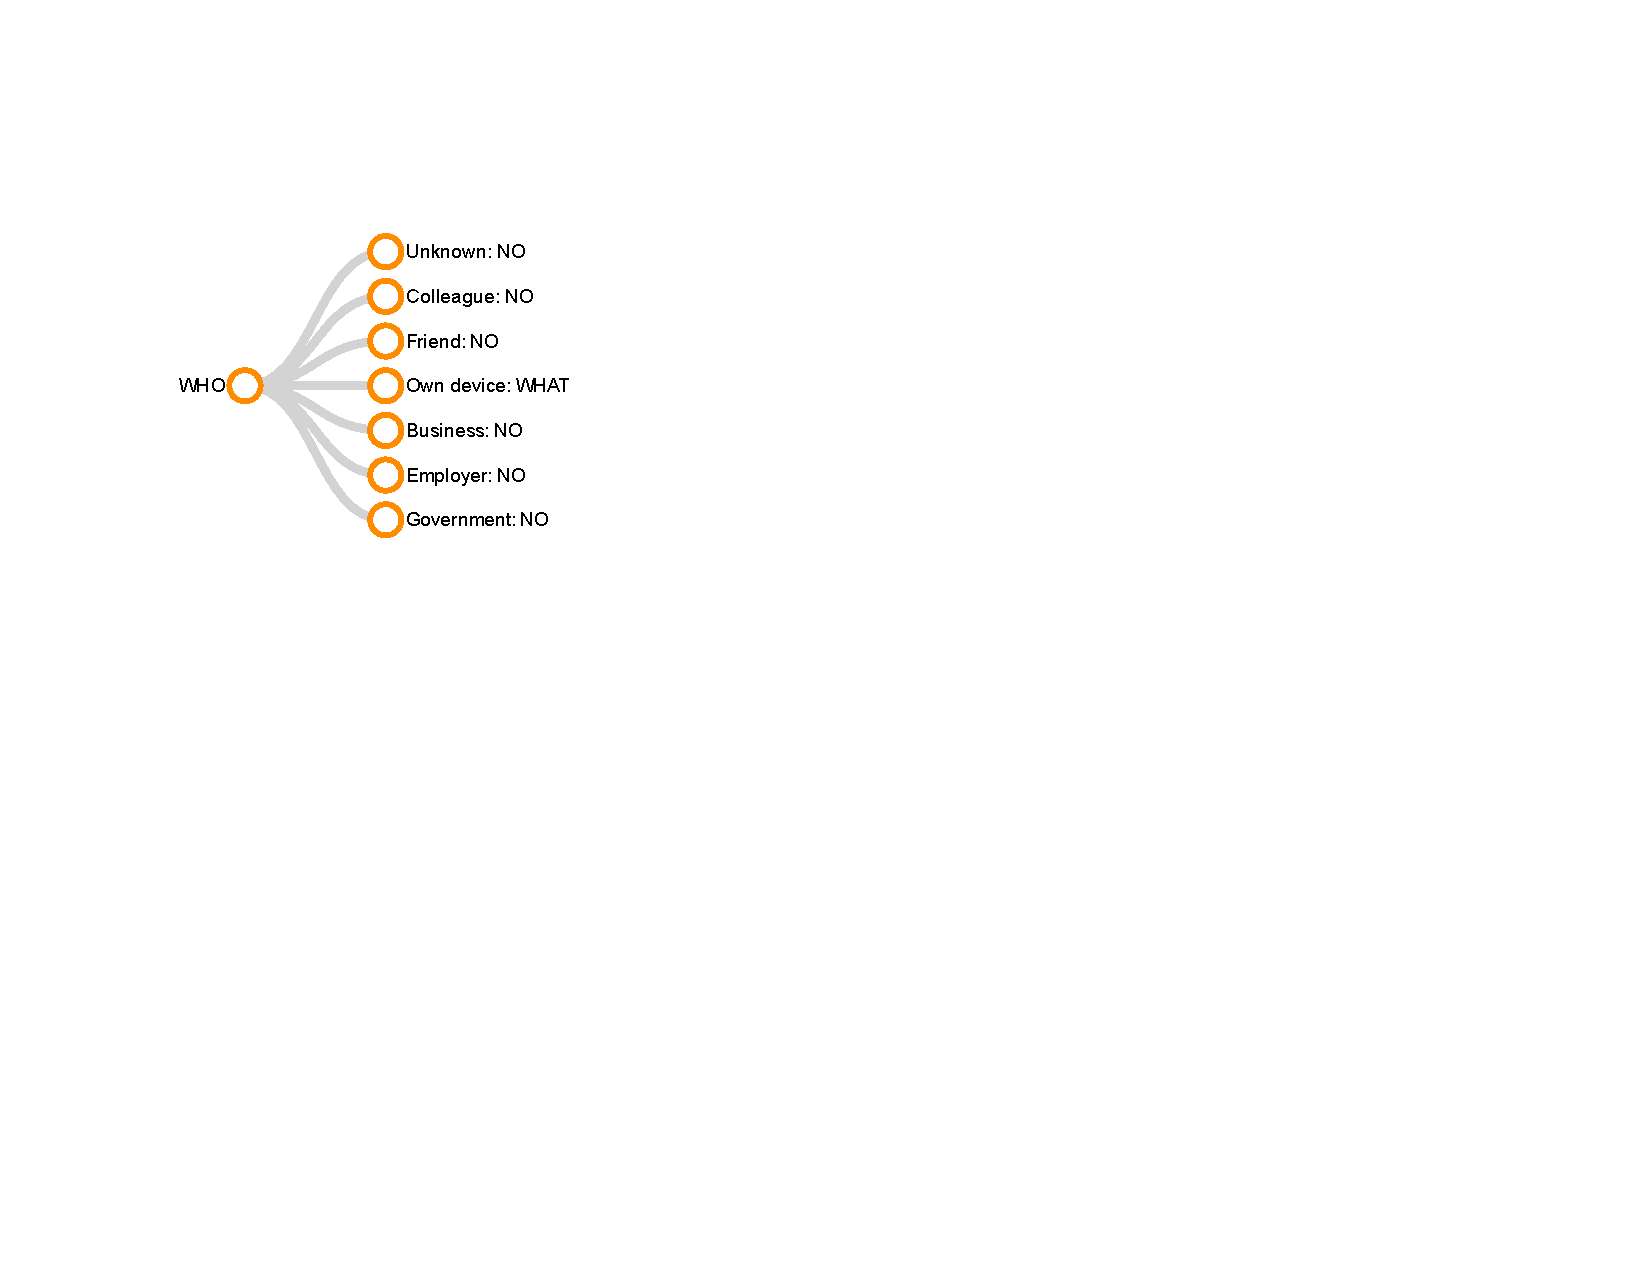
\includegraphics[width=.22\textwidth]{figures/overall.pdf}
	\caption{The Overall Prediction decision tree. Further drill down for `who' = `Own device' is provided in Table~\ref{tab:decisions}}
	\label{fig:naive_cls}
\end{figure}

\begin{table}
	\centering
	\caption{Drill down of the Overall Prediction tree for `who' = `Own device'}
	\label{tab:decisions}
	\begin{tabular}{ l | l }
		\hline
		\textbf{What} & \textbf{Decision} \\ \hline
		PhoneID				& Yes			\\
		PhoneID$>$identity 	& Yes			\\
		Location 			& No			\\
		Location$>$presence 	& Reason
		$\left\{
		\begin{tabular}{l | l}
		Safety & Yes \\ 
		Commercial & Yes \\
		Social-related & No \\
		Convenience & No \\
		Health-related & Yes \\
		None & Yes \\
		\end{tabular}\right.$ \\
		Voice 				& No			\\
		Voice$>$gender 		& Where 
		$\left\{
		\begin{tabular}{l | l}
		Your place & No\\
		Someone else & No \\
		Semi-public & No \\
		Public & Yes \\
		\end{tabular}\right.$ \\
		Voice$>$ age 			& No			\\
		Voice$>$identity 		& Yes			\\
		Voice$>$presence 		& Yes			\\
		Voice$>$mood 			& Yes			\\
		Photo 				& No			\\
		Photo$>$gender 		& No			\\
		Photo$>$age 			& No			\\
		Photo$>$identity 		& Yes			\\
		Photo$>$presence 		& No			\\
		Photo$>$mood 			& No			\\
		Video 				& No			\\
		Video$>$gender 		& No			\\
		Video$>$age 			& No			\\
		Video$>$presence 		& No			\\
		Video$>$mood 			& Yes			\\
		Video$>$looking at 	& Persistence
		$\left\{
		\begin{tabular}{l | l}
		Once & Yes \\
		Continuous & No \\
		\end{tabular}\right.$ \\
		Gaze 				& No			\\
		Gaze$>$looking at 	& Reason
		$\left\{
		\begin{tabular}{l | l}
		Safety & Yes \\
		Commercial & No \\
		Social-related & No \\
		Convenience & Yes \\
		Health-related & Yes \\
		None & Yes \\
		\end{tabular}\right.$ \\
	\end{tabular}
\end{table}


\subsection{Attitude-Based Clustering}
Our first ``smart profile'' solution uses the attitudes (comfort, risk, appropriateness) participants expressed for each scenario on a 7-point scale. We averaged the values per attitude across each participant's 14 answers, and ran $k$-means clustering on that data with 2, 3, 4 and 5 clusters. We then added participants' cluster assignments to our original dataset, and ran the J48 decision tree learner on the dataset with the additional \textbf{cluster} attribute. Accuracies of the resulting solutions are reported in Table~\ref{tab:comp_approach} under ``attitude-based clustering''.


All of the resulting trees had \textbf{cluster} as the root node. This indicates that this parameter is a very effective parameter for predicting users' decisions. This also allows us to split the trees at the root node, and create separate default settings for each cluster.

The 2-cluster solution (Figure~\ref{fig:2clusters}) has a 75.28\% accuracy --- a 3.0\% improvement over the ``smart default''. This solution results in one profile with `no' for everything, while for the other profile the decision depends on the recipient (\textbf{who}). This profile allows any collection involving the user's `Own device', and may allow collection by a `Friend' or an `Employer/School', depending on \textbf{what} is being collected.

\begin{figure}
	\centering
	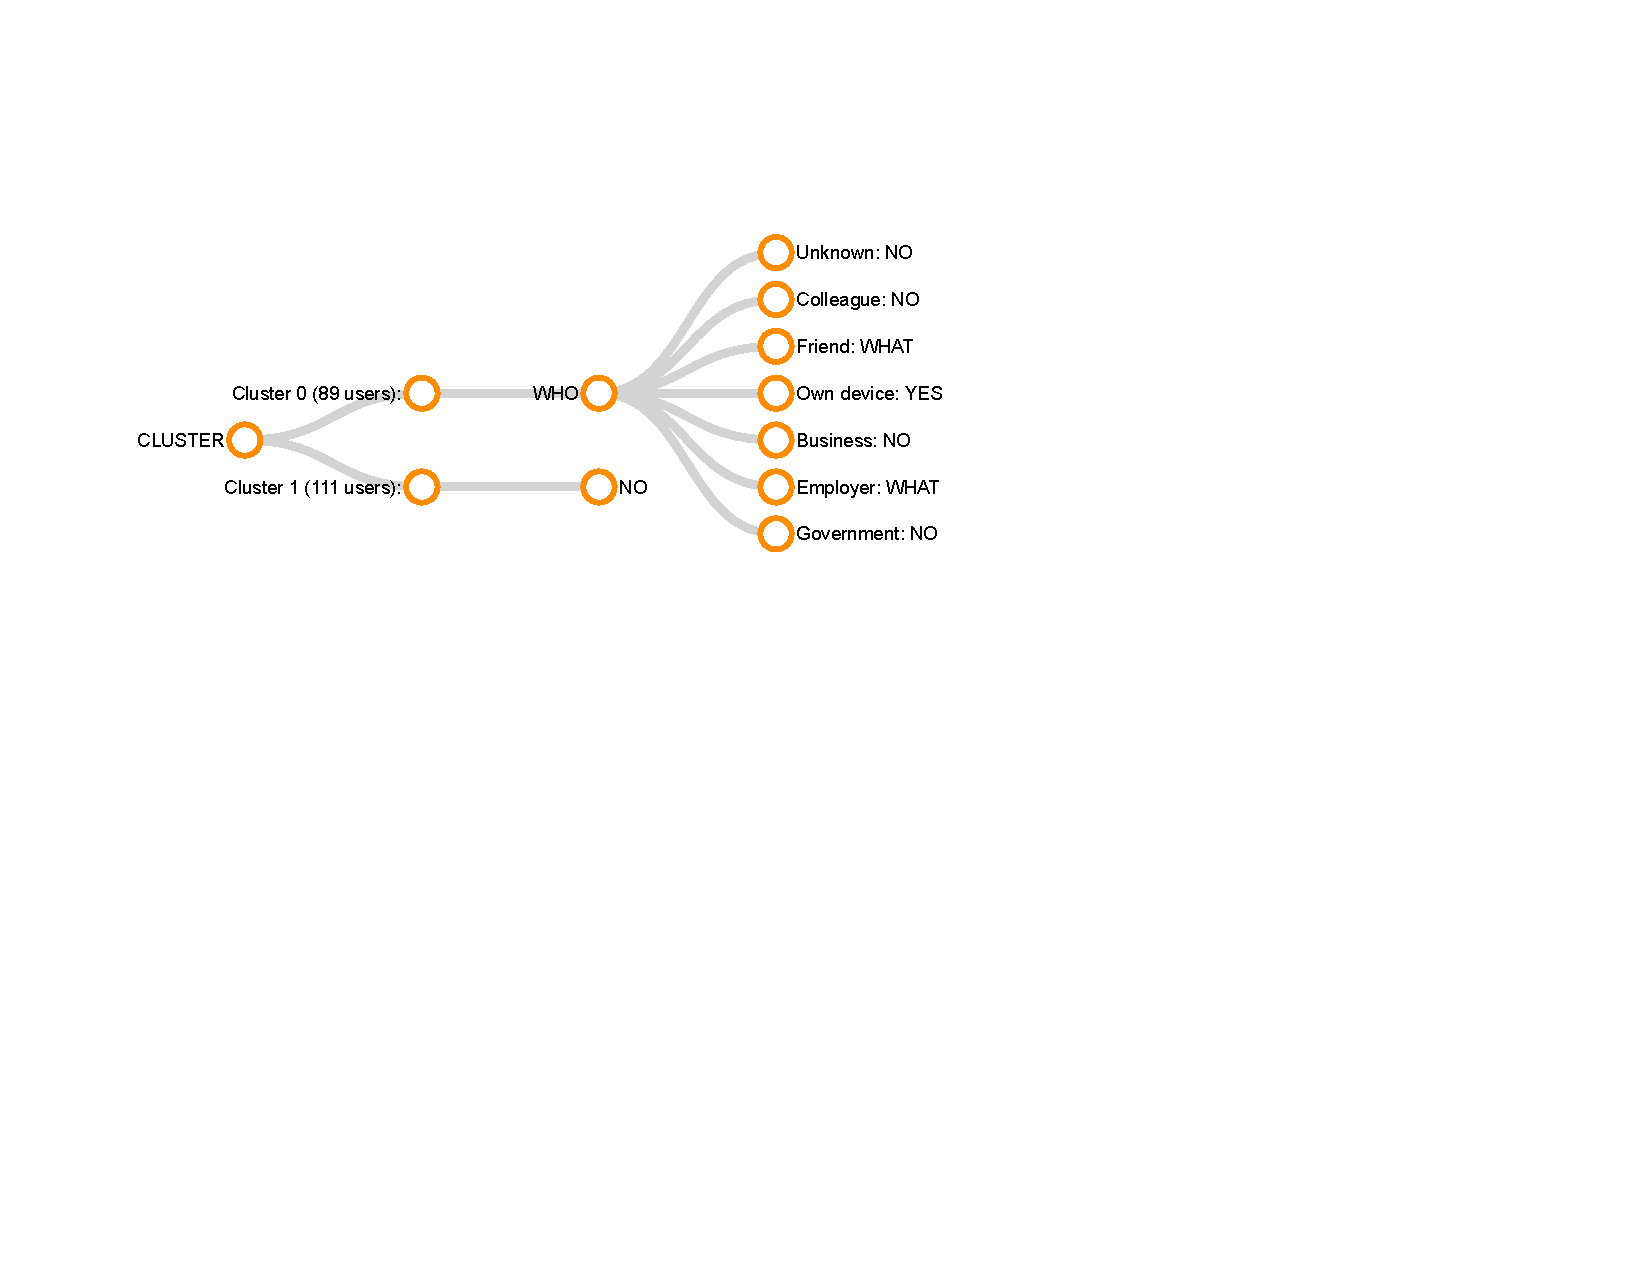
\includegraphics[width=0.8\textwidth]{figures/attitude-based-2.pdf}
	\caption{Attitude-based clustering: 2-cluster tree. Further drill down for \textbf{who} = `Friend' or `Employer/School' in Cluster 0 is hidden for space reasons.}
	\label{fig:2clusters}
\end{figure}

The 3-cluster solution has a slightly lower accuracy of 75.17\%, but is more parsimonious than the 2-cluster solution. There is one profile with `no' for everything, one profile that allows collection by the user's `Own device' only, and one profile that allows any collection except when the recipient is `Unknown' or the `Government'. The 4- and 5-cluster solutions have several clusters with the same sub-tree, and therefore reduce to a 3-cluster solution with 75.60\% and 75.25\% accuracy, respectively.


\begin{figure}
	\centering
	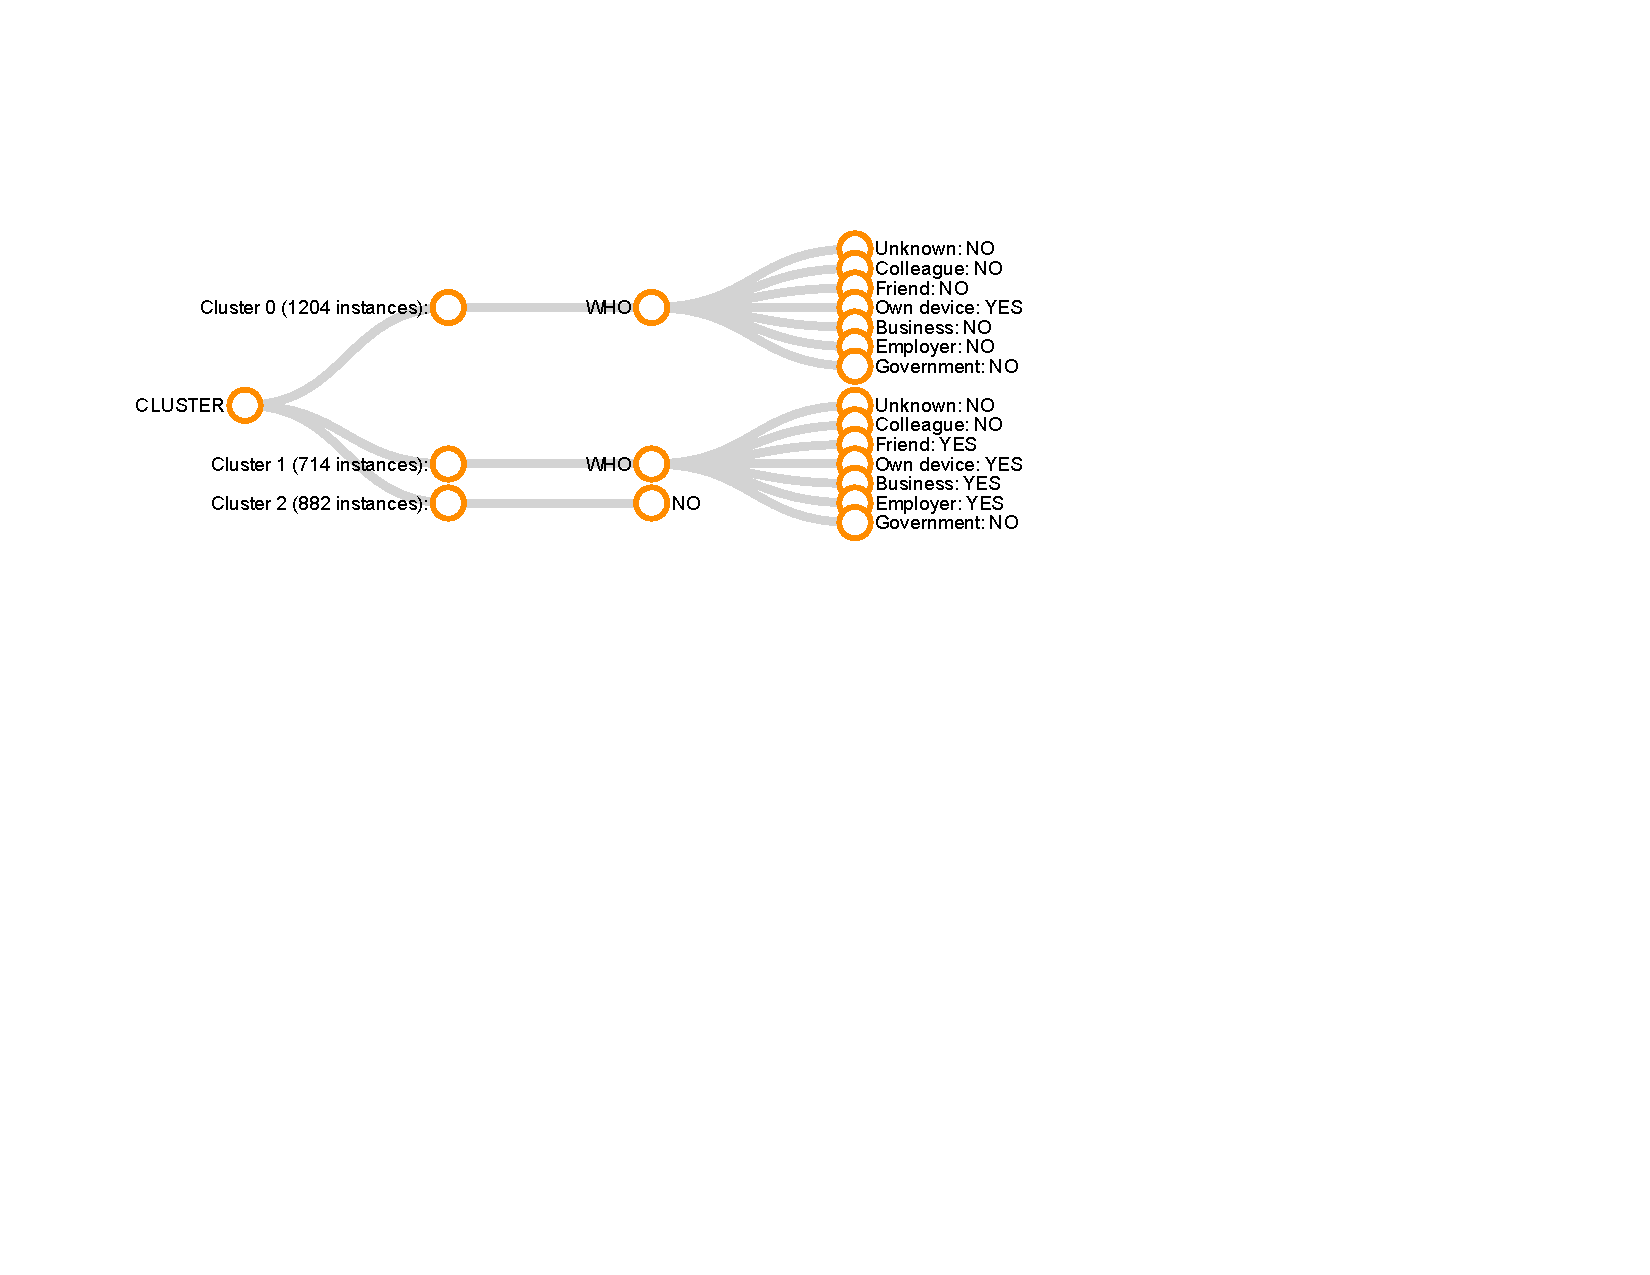
\includegraphics[width=0.8\textwidth]{figures/attitude-based-3.pdf}
	\caption{Attitude-based clustering: 3-cluster tree}
	\label{fig:3clusters}
\end{figure}


%\subsection{Trait-based clustering}
%Our second ``smart profile'' solution uses the 13 subjective questions asked towards the end of the survey conducted by Lee and Kobsa~\cite{lee2016understanding} regarding participants' privacy concerns, mobile Internet usage, and tech savviness. Confirmatory Factor Analysis was performed to extract latent traits from these questions, followed by a Factor Mixture Analysis to cluster participants on these traits into 2, 3, 4 or 5 clusters. We added the cluster assignments to the original dataset, and ran the J48 decision tree learner on the expanded dataset. Accuracies of the resulting solutions are reported in Table~\ref{tab:comp_approach} under ``trait-based clustering''.
%
%The attribute \textbf{cluster} ended up as root node only in the 2-cluster solution. This solution (Figure~\ref{fig:2clustersAtd}) was the best solution, but with an accuracy of 75.57\% it was not as good as the attitude-based clustering solutions. In this solution, one of the profiles does not allow any collection, while the other profile allows only collection by the user's `Own device'.
%
%The 3-, 4-, and 5-cluster solutions have several clusters with the same sub-tree, and reduce to a 2-cluster solution with 75.57\% and 75.07\% accuracy, respectively.
%
%\begin{figure}
%	\centering
%	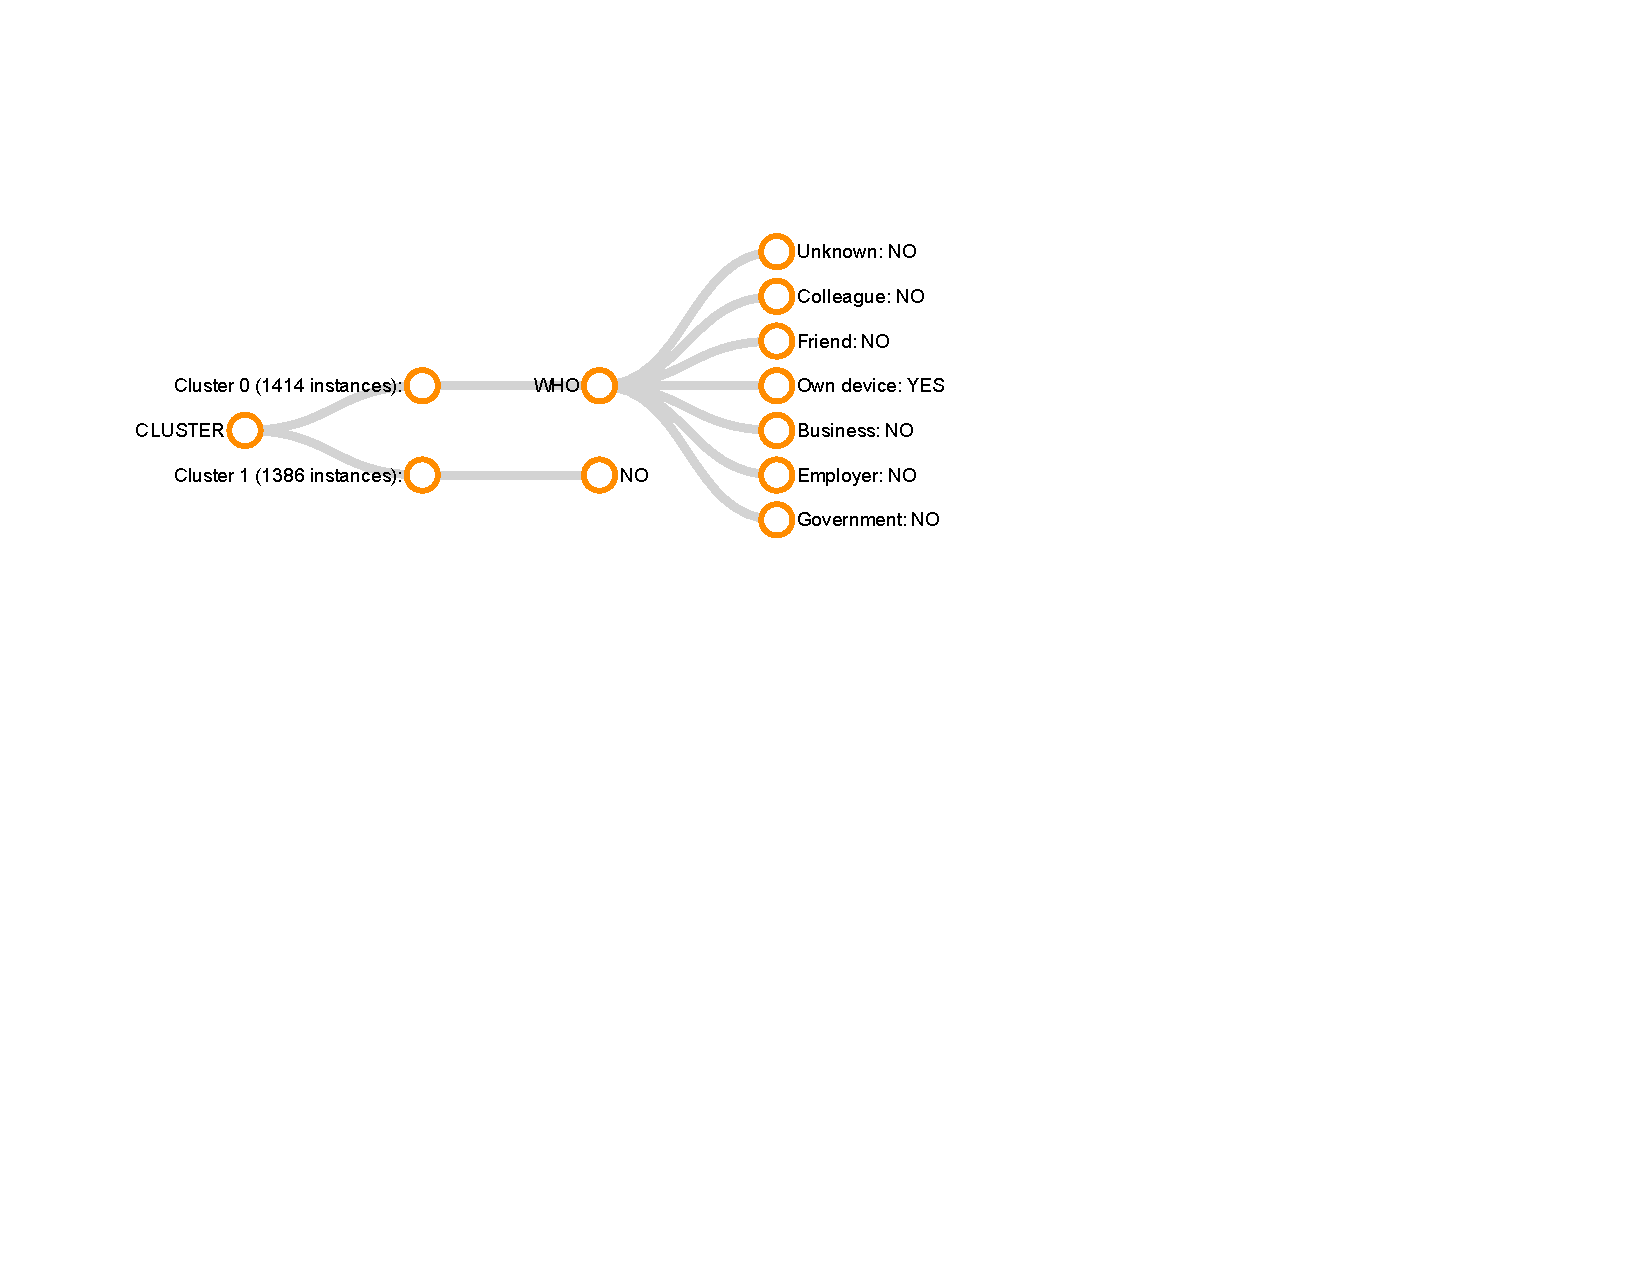
\includegraphics[width=0.48\textwidth]{figures/trait-based-2.pdf}
%	\caption{Trait-based clustering: 2-cluster tree}
%	\label{fig:2clustersAtd}
%\end{figure}




\subsection{Fit-based clustering}
Our fit-based clustering approach clusters participants without using any additional information. It instead uses the fit of the tree models to bootstrap the process of sorting participants into clusters. Like many bootstrapping methods, ours uses \emph{random starts} and \emph{iterative improvements} to find the optimal solution. The process is depicted in Figure~\ref{fig:flow_chart_fit}, and described in detail below. Accuracies of the resulting solutions are reported in Table~\ref{tab:comp_approach} under ``fit-based clustering''.

\begin{figure}[htp]
	\centering
	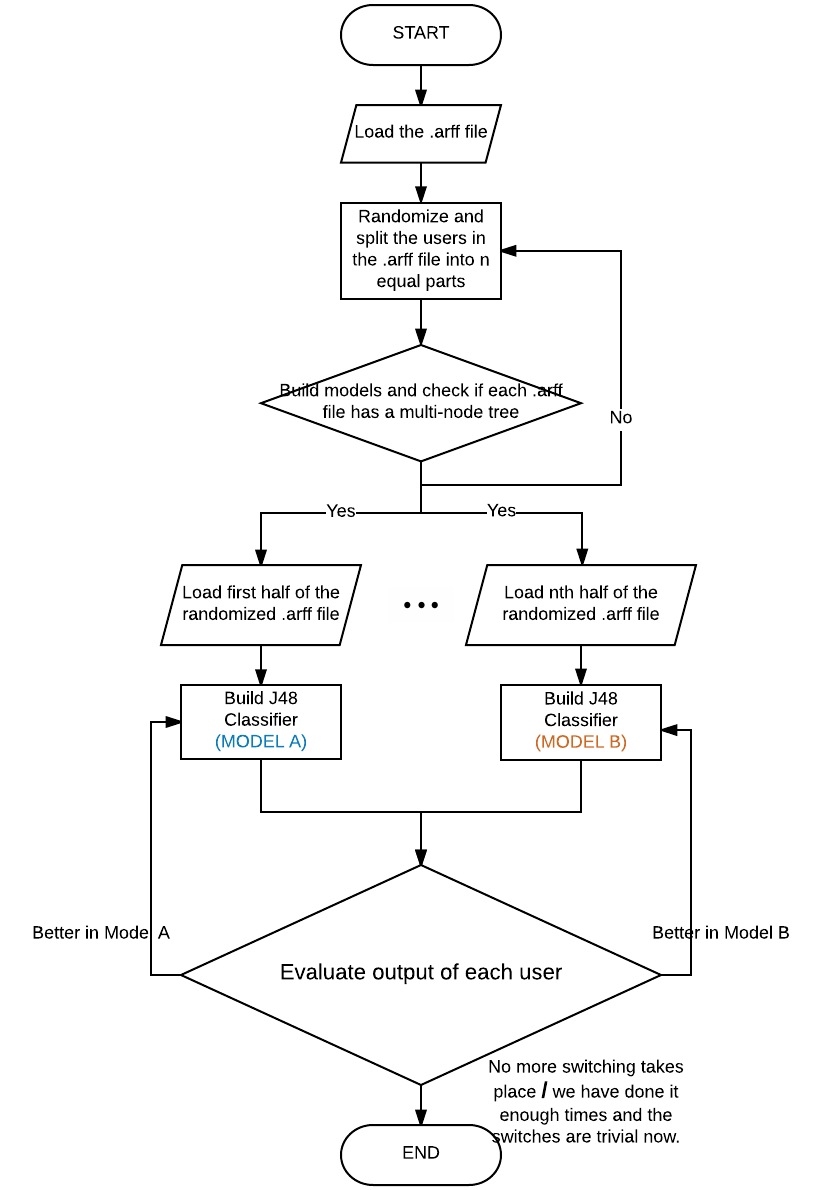
\includegraphics[width=0.8\textwidth]{figures/flowchartFit.png}
	\caption{The Flow Chart for Fit-based Clustering}
	\label{fig:flow_chart_fit}
\end{figure}

\textbf{Random starts:} We randomly divide particpants over $N$ separate groups, and learn a tree for each group. This is repeated until a non-trivial starting solution (i.e., with distinctly different trees per cluster) is found. 

\textbf{Iterative improvements:} Once each of the $N$ groups has a unique decision tree, we evaluate for each participant which of the trees best represents their 14 decisions. If this is the tree of a different group, we switch the participant to this group. Once all participants are evaluated and put in the group of their best-fitting tree, the tree in each group is re-learned with the data of the new group members. This then prompts another round of evaluations, and this process continues until no further switches are performed. 

Since this process is influenced by random chance, it is repeated in its entirety to find the optimal solution. Cross-validation is performed in the final step to prevent over-fitting. Accuracies of the 2- and 3-cluster solutions are reported in Table~\ref{tab:comp_approach} under ``fit-based clustering''. We were not able to converge on a higher number of clusters. 

The 2-cluster solution has a 77.99\% accuracy---a 6.7\% improvement over the ``smart default''. One profile has `no' for everything, while the settings in the other profile depends on \textbf{who}: it allows any collection by the user's `Own device', and may allow collection by a `Friend's device' or an `Employer', depending on \textbf{what} is collected.


%\begin{figure}
%	\centering
%	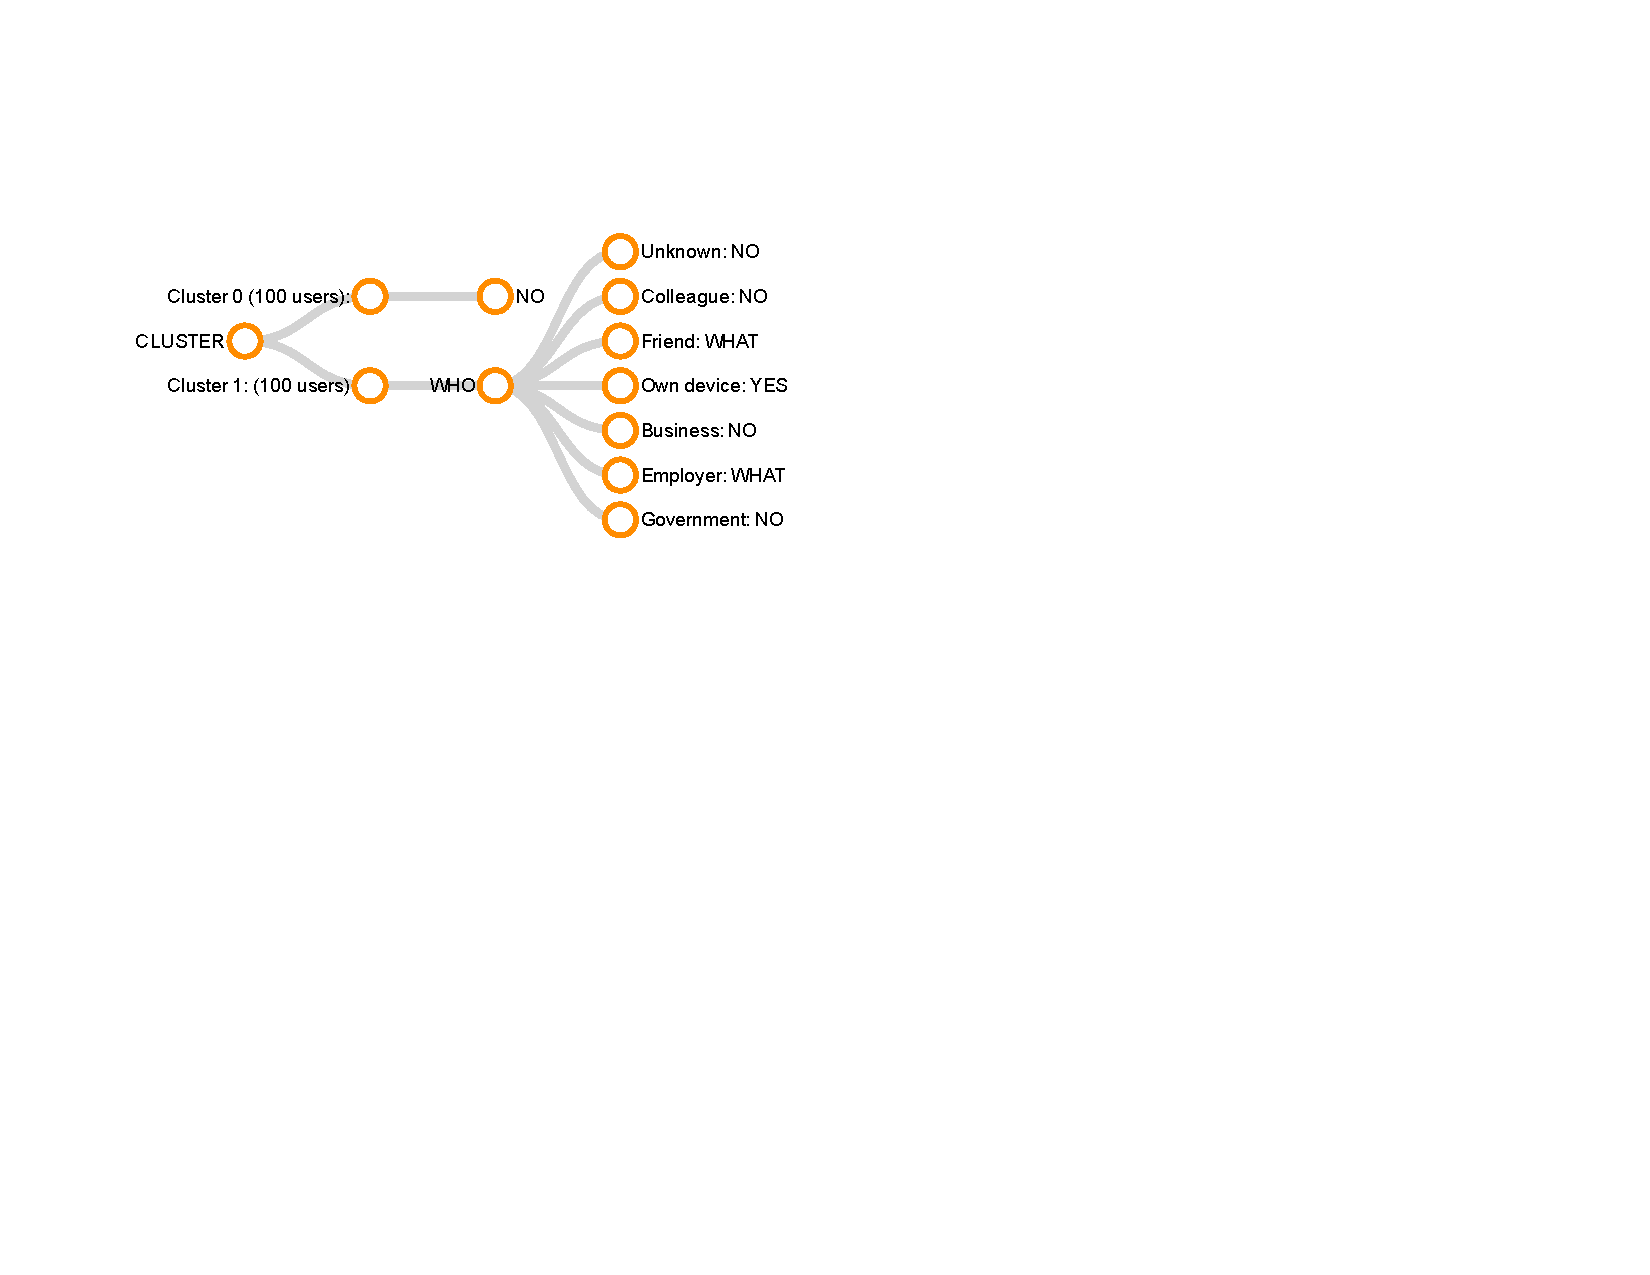
\includegraphics[width=.42\textwidth]{figures/fit-based-2c.pdf}
%	\caption{Fit-based clustering: 2-cluster tree. Further drill down for \textbf{who} = `Friend' or `Employer/School' in Cluster 1 is hidden for space reasons.}
%	\label{fig:2clustersFit}
%\end{figure}

The 3-cluster solution (Figure~\ref{fig:3clustersFit}) has a 81.54\% accuracy --- an 11.5\% improvement over the ``smart default''. We find one profile with `no' for everything; one profile that may allow collection by the user's `Own device', depending on \textbf{what} is being collected; and one profile that allows any collection except when the recipient (\textbf{who}) is `Unknown', the `Government', or a `Colleague', with settings for the latter depending on the \textbf{reason}.

\begin{figure*}
	\centering
	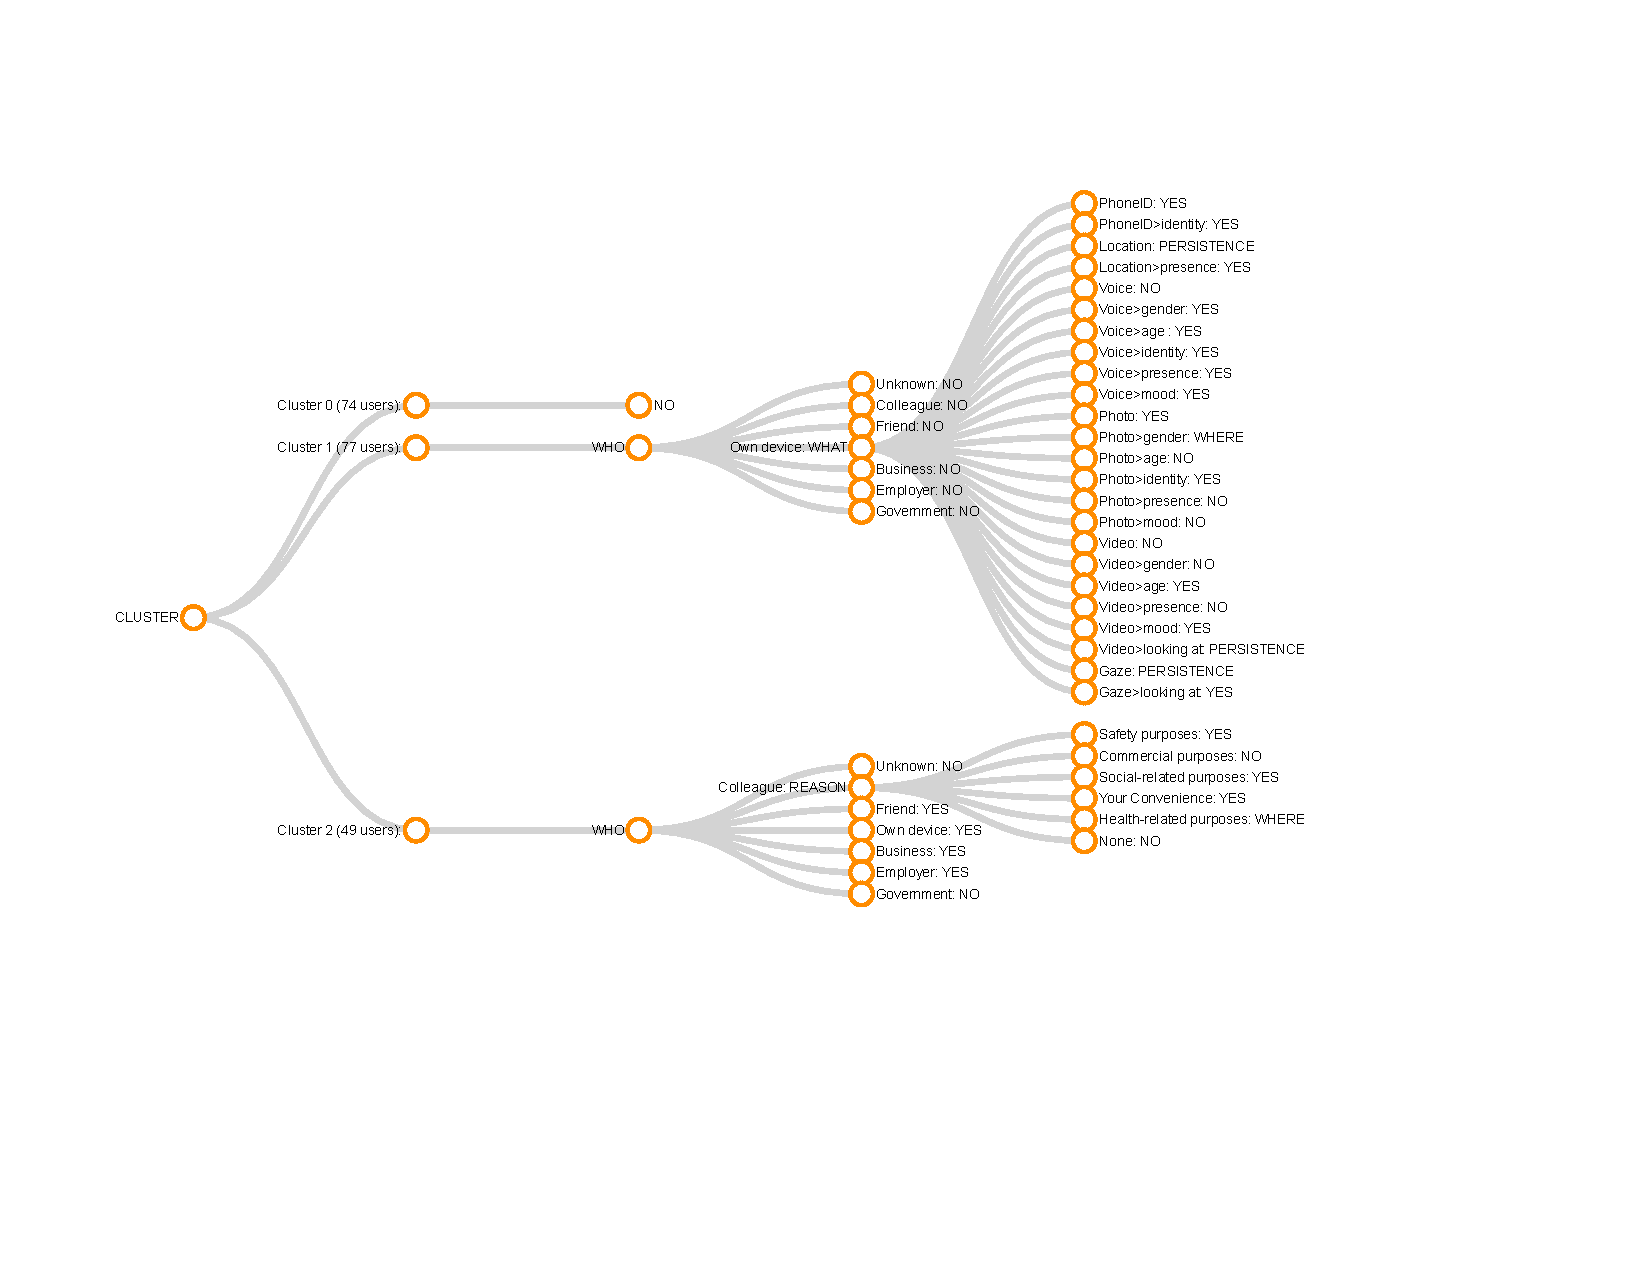
\includegraphics[width=\textwidth]{figures/fit-based-3c.pdf}
	\caption{Fit-based clustering: 3-cluster tree. Further drill down is hidden for space reasons.}
	\label{fig:3clustersFit}
\end{figure*}

\subsection{Agglomerative clustering}
Our final method for finding ``smart profiles'' follows a hierarchical bottom-up (or agglomerative) approach. It first fits a separate tree for each participant, and then iteratively merges them based on similarity. 156 of the initial 200 trees predict ``no for everything'' and 34 of them predict ``yes for everything''---these are merged first. For every possible pair of the remaining 10 trees, the accuracy of the pair is compared with the mean accuracy the individual trees, and the pair with the smallest reduction in accuracy is merged. This process is repeated until we reach the predefined number of clusters.

We were able to reach a 5- and 4-cluster solution. The 3-cluster solution collapsed down into a 2-cluster solution with one profile of all `yes'es and one profile of all `no's (a somewhat trivial solution with a relatively bad fit). Accuracies of the 4- and 5-cluster (Table~\ref{tab:comp_approach}, ``agglomerative clustering'') are 78.13\% and 78.27\% respectively. For the 4-cluster solution, we find one profile with `no' for everything, one profile with `yes' for everything, one profile that depends on \textbf{who}, and another that depends on \textbf{what}. The latter two profiles drill down even further on specific values of \textbf{who} and \textbf{what}, respectively.



\begin{figure}[t]
	\centering
	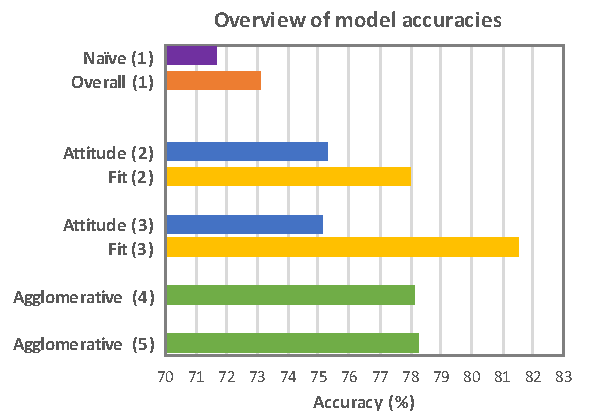
\includegraphics[width=0.43\textwidth]{figures/compare.pdf}
	\caption{Accuracy of our clustering approaches}
	\label{fig:comp_approach}
\end{figure}

\subsection{Discussion of Machine Learning Results}
Figure~\ref{fig:comp_approach} shows a comparison of the presented approaches. Compared to a naive default setting (all `no'), a ``smart default'' makes a 2.0\% improvement. The fit-based 2-cluster solution results in two ``smart profiles'' that make another 6.7\% improvement over the ``smart default'', while the three ``smart profiles'' of the fit-based 3-cluster solution make an 11.5\% improvement. If we let users choose the best option among these three profiles, they will on average be content with 81.54\% of the settings. This rivals the accuracy of some of the ``active tracking'' machine learning approaches~\cite{sadeh2009understanding}.

In line with our statistical results, the factor \textbf{who} seems to be the most prominent parameter, followed by \textbf{what}. In some cases the settings are more complex, depending on a combination of \textbf{who} and \textbf{what}. This is in line with the interaction effect observed in our statistical results.

Even our most accurate solution is not without fault, and its accuracy depends most on the \textbf{who} parameter. Specifically, the solution is most accurate for the user's own device, the device of a friend, and when the recipient is unknown. It is however less accurate when the recipient is a colleague, a nearby business, an employer, or the government. In these scenarios, more misclassifications tend to happen, so it would be useful to `guide' users to specifically have a look at these default settings, should they opt to make any manual overrides.

\section{Privacy-setting Prototypes (original work)}\label{sec:design1}
In Section~\ref{sec:sa1}, we developed a ``layered" interface that general IoT users can use to manually set their privacy settings (see Figure~\ref{fig:interface1}). Our machine learning analysis (Section~\ref{sec:predict1}) resulted in a number of interesting solutions for ``smart profiles'' that would allow users of this interface to set their privacy settings with a single click (i.e., a choice of profile). In this section we therefore present how we integrate the ``smart profiles" with our prototype. 

\subsection{Smart Default Setting}
The design of ``layered" interface is based on our statistical results that there exists no interaction effect between the parameters, our ``smart default" settings can be integrated to this prototype in nature. For ``yes to everything'' or ``no to everything'' default, we can just simply set all the settings in the Screen 4 of Figure~\ref{fig:interface1} to all `on' or `off'.

For the results from our Overall Prediction (see Figure~\ref{fig:naive_cls}), we can create a ``smart default'' setting that is 73.10\% accurate on average. In this version, the IoT settings for all devices are set to `off', except for `My own device', which will be set to the middle option. Table~\ref{tab:decisions} shows the default settings at deeper levels.
As this default setting is on average only 73.10\% accurate, we expect users to still change some of their settings. They can do this by navigating the manual settings interface.

\subsection{Smart Profiles}
To improve the accuracy of the default setting, we can instead build two ``smart profiles'', and allow the user to choose among them. Using the 3-cluster solution of the fit-based approach (see Figure~\ref{fig:3clustersFit}), we can attain an accuracy of 81.54\%. Screen 1 in Figure~\ref{fig:interface1} shows a selection screen where the user can choose between these profiles. The ``Limited collection'' profile allows the collection of any information by the user's own devices, their friends' devices, their employer/school's devices, and devices of nearby businesses. Devices of colleagues are only allowed to collect information for certain reasons. The ``Limited collection, personal devices only'' profile only allows the collection of certain types of information by the user's own devices. The ``No collection'' profile does not allow any data collection to take place by default.

Once the user chooses a profile, they will move to the manual settings interface (Screens 2--4), where they can further change some of their settings.

\begin{figure}[htb]
	\centering
	\begin{subfigure}[t]{0.24\textwidth}
		\centering
		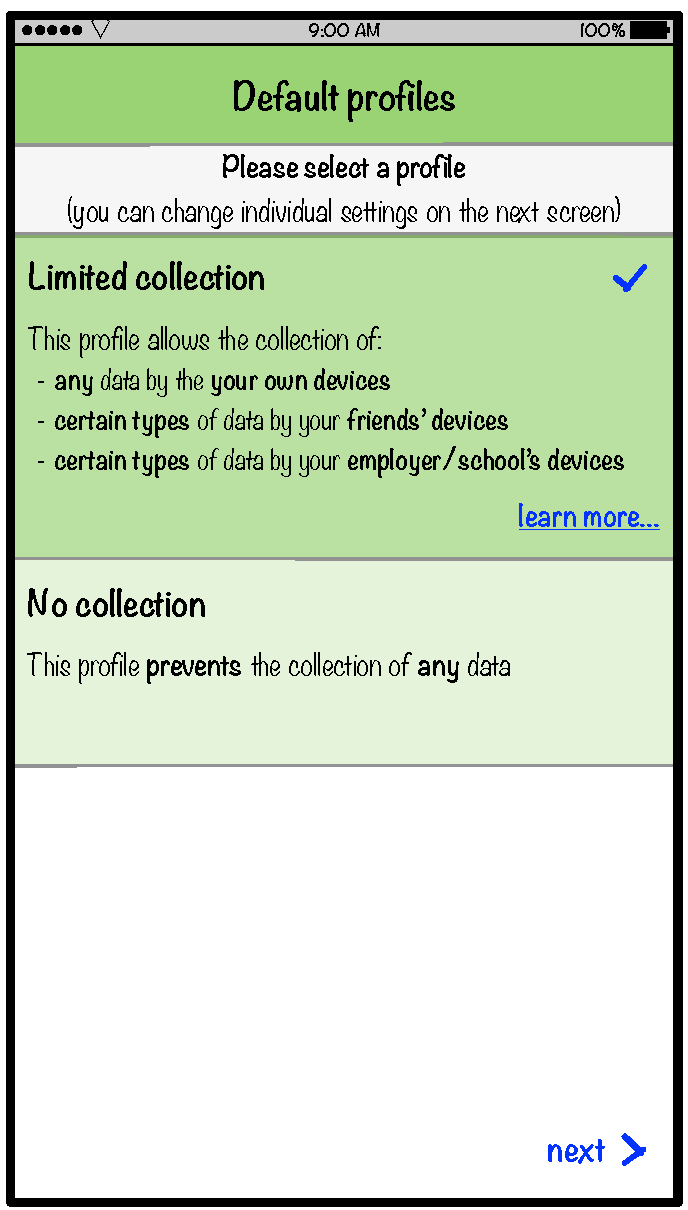
\includegraphics[height=2.8in]{figures/profiles2.pdf}
		\caption{2-profile choice interface}
		\label{fig:2profile_default_setting}
	\end{subfigure}%
	~~~~~~~~~
	\begin{subfigure}[t]{0.24\textwidth}
		\centering
		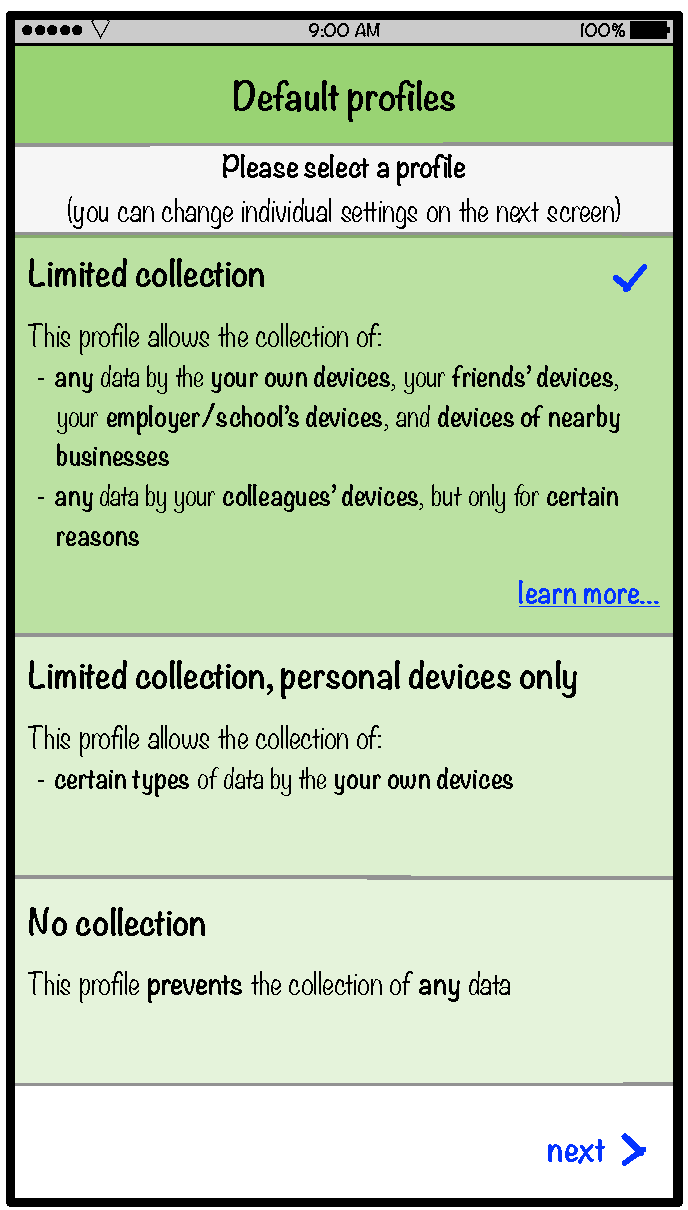
\includegraphics[height=2.8in]{figures/profiles3.pdf}
		\caption{3-profile choice interface}
		\label{fig:3profile_default_setting}
	\end{subfigure}%
	\caption{Two types of profile choice interfaces}
\end{figure}

\section{Summary}
In this chapter, we have presented the following:

\begin{itemize}
	\item Using statistical analysis, uncover the relative importance of the parameters that influence users' privacy decisions. Develop a ``layered interface'' in which these parameters are presented in decreasing order of importance.
	\item Using a tree-learning algorithm, create a decision tree that best predicts participants' choices based on the parameters. Use this tree to create a ``smart default'' setting.
	\item Using a combination of clustering and tree-learning algorithms, create a set of $N$ decision trees that best predict participants' choices. Use the trees to create $N$ ``smart profiles''.
	\item Develop a prototype for an IoT privacy-setting interface that integrates the layered interface with the smart default or the smart profiles.
\end{itemize}

Our statistical and machine learning results both indicated that recipient of the information (\textbf{who}) is the most significant parameter in users' decision to allow or reject IoT-based information collection. This parameter therefore features at the forefront in our layered settings interface, and plays an important role in our smart profiles. The \textbf{what} parameter was the second-most important decision parameter, and interacted significantly with the \textbf{who} parameter. This parameter therefore features at the second level of our settings interface, and further qualifies some of the settings in our smart profiles.

Our layered interface allows a further drill-down to the \textbf{reason} and \textbf{persistence} parameters, but given the relatively lesser importance of these parameters, we expect few users to engage with the interface at this level. Moreover, the \textbf{where} parameter was not significant, so we left it out of the interface.

While a naive (`no' to all) default setting in our interface would have provided an accuracy of 71.67\%, it would not have allowed users to reap the potential benefits associated with IoT data collection without changing the default setting. Our Overall Prediction procedure resulted in a smart default setting that was a bit more permissive, and increased the accuracy by 2\%.

The fit-based clustering approach, which iteratively clusters users and fits an optimal tree in each cluster, provided the best solution. This resulted in an interface where users can choose from 3 profiles, which increases the accuracy by another 11.5\%.

The scenario-based method presented in this paper is particularly suited for novel domains where few real interaction exist. We note, though, that this novelty may hamper our approach: users' decisions are inherently limited by the knowledge they have about IoT. Lee and Kobsa~\cite{lee2016understanding} made sure to educate users about the presented scenarios, hence their data is arguably better in this regard than data from ``live'' systems. However, as the adaptation of IoT becomes more widespread, the mindset and knowledge regarding such technologies---and thus their privacy preferences---might change. Our ``smart profiles'' may thus eventually have to be updated in future work, but for now, our current profiles can at least help users make make better privacy decisions in their initial stages of usage.

Our analysis allowed us to use \emph{data-driven design} to bootstrap the development of a privacy-setting interface, but a future user experiment could investigate whether users are comfortable with the layered interface, and whether they prefer a single ``smart default'' setting or a choice among ``smart profiles''.

In the next chapter, we discuss the challenges and solutions when we extended work that we have done in the domain of household IoT ("smart home") domain.

	% !TeX root = proposal.tex
\chapter{Recommending Privacy Settings for Household IoT}\label{chapter:householdIoT}

In Chapter~\ref{chapter:generalIoT}, we have discussed recommending privacy preference for general IoT users. In this chapter, we present the work completed to date in the areas of designing for privacy for Household IoT. We expand and improve upon the previously-developed data-driven approach to design privacy-setting interfaces for users of household IoT devices. Moving the context to a more narrow environment shifts the focus of the privacy decision from the entity collecting information (which was the dominant parameter in our previous work) to a more contextual evaluation of the content or nature of the information ~\cite{nissenbaum_privacy_2004}. 

\section{Experimental Setup}\label{sec:exp_setup}
In Chapter~\ref{chapter:generalIoT}, we found that "where" does not have significant effect on disclosure decisions; also the usage environment of household IoT systems/devices are always in users' home. Moreover, the structure of users' houses are different from case to case, it would be too complicated if we define "where" to a more finer-granulated level, such as bedroom, kitchen, etc.,  Hence there there is no need to retain the parameter "where". ``Persistence" of tracking is more relevant in public IoT, where encounters are often ephemeral, hence persistent tracking is less common than in household IoT. ``Storage" and ``Action" allow us to explore secondary uses of the information; something we learned from the qualitative feedback in our previous study was a prominent concern among users.

Because of the above reasons, we conducted a new user study focusing on household IoT in particular, and further refine our approach to allow us to create more carefully tailored user interfaces. In this section, we first discuss the factorial procedure by which we developed 4608 highly specific IoT scenarios, as well as the questions we asked participants to evaluate these scenarios. We then describe the participant selection and experimental procedures used to collect over 13500 responses from 1133 participants.

\subsection{Contextual Scenarios}
The scenarios evaluated in our study are based on a full factorial combination of five different Parameters: Who, What, Purpose, Storage and Action. A total of $8(who)*12(what)*4(purpose)*4(storage)*3(action) = 4608$ scenarios were tested this way. 

The scenarios asked participants to imagine that they were owners and active users of the presented IoT devices, trying to decide whether to turn on or off certain functionalities and/or data sharing practices. To avoid endowment effects, the scenarios themselves made no indication as to whether the functionality was currently turned on or off (such endowment effects were instead introduced by manipulating the framing of the Decision question; see section \ref{sec:questions}). An example scenarios is: \emph{``Your smart TV (Who) uses a camera (What) to give you timely alerts (Purpose). The data is stored locally (Storage) and used to optimize the service (Action).''} This scenario may for example represent a situation where the smarthome system has detected (via camera) a delivery of package and then alerts the user (via the smart TV) about its arrival. In this particular scenario we note that the video data is stored locally to optimize service; this could mean that the smarthome system uses the video stream to (locally) train a package detection algorithm. Similarly, another example of scenario is: \emph{``Your Smart Assistant uses a microphone to detect your location in house. The data is stored on a remote server and shared with third parties to recommend you other services.''} Similarly, this scenario could represent a situation where the smarthome has detected (via microphone) it's user's location in the house and this information is shared to smart assistant. In the scenario, the data is stored on remote server and shared with third parties so that it can recommend additional services (like weather or local transportation) via third parties to the user.

The levels of all five parameters used in our experiment are shown in Table~\ref{tab:parameter2}. The parameters were highlighted in the scenario for easy identification, and upon hovering the mouse cursor over them each parameter would show a succinct description of the parameter. %\textcolor{blue}{Figure~\ref{fig:scenario} in the Appendix shows a screenshot of a scenario as shown to participants in the study.}
A thirteenth scenario regarding the interrelated control of various IoT devices (e.g. \emph{``You can use your smart TV to control your smart refrigerator''}) was also asked, but our current analysis focuses on the information-sharing scenarios only.

\subsection{Scenario Evaluation Questions}
\label{sec:questions}
The first question participants were asked about each scenario was whether they would enable or disable the particular feature mentioned in scenario (Decision). Subsequently, they were asked about their attitudes regarding the scenario in terms of their perceived Risk, Appropriateness, Comfort, Expectedness and Usefulness regarding the presented scenario (e.g., \emph{``How appropriate do you think this scenario is?''}). These questions were answered on a 7-point scale (e.g., \emph{``very inappropriate''} to \emph{``very appropriate''}). In every 4th scenario, the Risk and Usefulness questions were followed by an open question asking the participants to describe the potential Risk and Usefulness of the scenario. We asked these question mainly to encourage participants to carefully evaluate the scenarios.%A screenshot of the questions asked about each scenario is depicted in Figure~\ref{fig:scenario} in the Appendix.

%In addition to the twelve scenarios, the participants were also presented with a 13th scenario. This scenario was focused on giving the participants an ability to control for collection of information by devices. This was done by changing the for \emph{Who} and \emph{What} parameters. However, the rest of the parameters were kept same while forming the scenario. 
The framing and default of the Decision question were manipulated between-subjects at three levels each: positive framing (``Would you enable this feature?'', options: Yes/No), negative framing (``Would you disable this feature?'', options: Yes/No) or neutral framing (``What would you do with this feature?'', options: Enable/Disable); combined with a positive default (enabled by default), negative default (disabled by default), or no default (forced choice).


\begin{table}
	\centering
	\caption{Parameters used to construct the information-sharing scenarios. The ``codes'' are used as abbreviations in graphs and figures throughout the paper and the Appendix.}
	\label{tab:parameter2}
	\begin{tabular} {l|l|l}
		\hline
		\textbf{Parameter} & \textbf{Levels} & \textbf{Code} 	 \\ \hline
		Who:  & 1. Home Security System & SS\\ 		
		\emph{Your Smart...}	& 2. Refrigerator & RE							 \\
		& 3. HVAC System							& HV	 \\
		& 4. Washing Machine						& WM		 \\
		& 5. Lighting System						& SL	 \\
		& 6. Assistant 							 &SA\\
		& 7. TV 							 &TV\\
		& 8. Alarm Clock							&SC \\ \hline
		What:  & 1. Home Security System & CSE\\
		\emph{...uses information } & 2. Refrigerator &CRE							 \\
		\emph{collected by your...} & 3. HVAC System &CHV								 \\
		& 4. Washing Machine						& CWA		 \\
		& 5. Lighting System						&CLI	 \\
		& 6. Assistant 							 & CAS\\
		& 7. TV 							 & CTV\\
		& 8. Alarm							 & CAL\\
		& 9. uses a location sensor			&CLO	\\	
		& 10. uses a camera				& CCA\\	
		& 11. uses a microphone			& CMP				\\	
		& 12. connects to your smart phone/watch &CSW				\\\hline
		Purpose : & 1. detect whether you are home & PH		\\
		\emph{...to...} & 2. detect your location in house &LH		\\				
		& 3. automate its operations &AO\\
		& 4. give you timely alerts & TA\\ \hline
		%Who (Control):& 1. Assistant \\
		%\emph{"You can use your} & 2. TV							 \\
		%\emph{Smart...} & 3. Alarm Clock								 \\
		%& 4. Phone/Watch								 \\\hline
		%What (Control): & 1. Home Security System \\
		%\emph{...to control your...} & 2. Refrigerator							 \\
		%& 3. HVAC System								 \\
		%& 4. Washing Machine								 \\
		%& 5. Lighting System							 \\
		%& 6. Assistant 							 \\
		%& 7. TV 							 \\
		%& 8. Alarm Clock							 \\ \hline
		Storage:  & 1. locally	& L\\
		\emph{The data is stored...} & 2. on remote server & R						\\
		& 3. on a remote server and & T\\
		& shared with third parties &\\\hline
		Action: & 1. optimize the service & O \\
		\emph{...and used to... } & 2. give insight into your behavior& I \\
		& 3. recommend you other services & R\\
		& 4. [None] & N\\ \hline
	\end{tabular}
\end{table}

\subsection{Participants and Procedures}
To collect our dataset, 1133 adult U.S.-based participants (53.53\% Female, 45.75\% Male, 8 participants did not disclose) were recruited through Amazon Mechanical Turk. Participation was restricted to Mechanical Turk workers with a high reputation (at least 50 completed tasks completed with an average accuracy greater than 95\%). Participants were paid \$2.00 upon successful completion of the study. The participants were warned about not getting paid in case they failed attention checks.

The study participants represented a wide range of ages, with 9 participants less than 20 years old, 130 aged 20-25, 273 aged 25-30, 418 aged 30-40, 175 aged 40-50, 80 aged 50-60, and 43 participants over 60 years old (5 participants did not disclose their age). This significant increase in participants over the Lee and Kobsa~\cite{lee2016understanding} dataset is commensurate with our expectation of more complex privacy decision behaviors in household IoT compared to public IoT.

Each participant was first shown a video with a brief introduction to various smart home devices, which also mentioned various ways in which the different appliances would cooperate and communicate within a home. After the video, participants were asked to answer three attention check questions. If they got any of these questions wrong, they would be asked to read the transcript of the video and re-answer the questions.

After the introduction video, each participant was presented with 12 information-sharing scenarios (and a 13th control scenario, not considered in this paper). These scenarios were selected from the available 4608 scenarios using fractional factorial design\footnote{The scenario assignment scheme is available at \url{https://www.usabart.nl/scenarios.csv}} that balances the within- and between-subjects assignment of each parameter's main effect, and creates a uniform exposure for each participant to the various parameters (i.e., to avoid ``runs'' of near-similar scenarios). Participants were asked to carefully read the scenario and then answer all questions about it. Two of the 13 scenarios had an additional attention check question (e.g., ``Please answer this question with Completely Agree'', and there was an additional attention check question asking participants about the remaining time to finish the study (which was displayed right there on the same page. Participants rushing through the experiment and/or repeatedly failing the attention check questions were removed from the dataset.
%
%\section{Inspecting Users' Decisions}\label{sec:inspect}
%In this section we explain the different regression analyses performed on the dataset to understand how different scenario parameters affected the decisions made by participants. We begin by explaining the effects of scenario parameters on participants' decision to enable or disable the feature mentioned in the scenario. Similar to Bahirat et. al., we also present the results of the mediation analysis, which are on the lines of attitude-behavior models~\cite{bahiratiui2018,ajzen1977attitude}. As shown in Figure~\ref{fig:mediation_test}, we test whether participants' attitudes mediate the effects of the scenario parameters on their decisions. This mediation analysis involves the following tests:
%
%\textbf{Test 1}: The effect of parameters (Who, What, Purpose, Storage, Action) on attitudes (Risk, Comfort, Appropriateness, Expectedness and Usefulness).
%
%\textbf{Test 2}: The effect of attitudes on decision.
%
%\textbf{Test 3}: The effect of both parameters \emph{and} attitudes on decision.
%
%If, tests 1 and 2 are significant and test 3 reveals a drastic reduction in the conditional direct effect of parameters, then we can say that the effects of scenario parameters on participant's decision are mediated by their attitudes~\cite{bahiratiui2018}.
%
%
%\begin{figure}
%	\centering
%	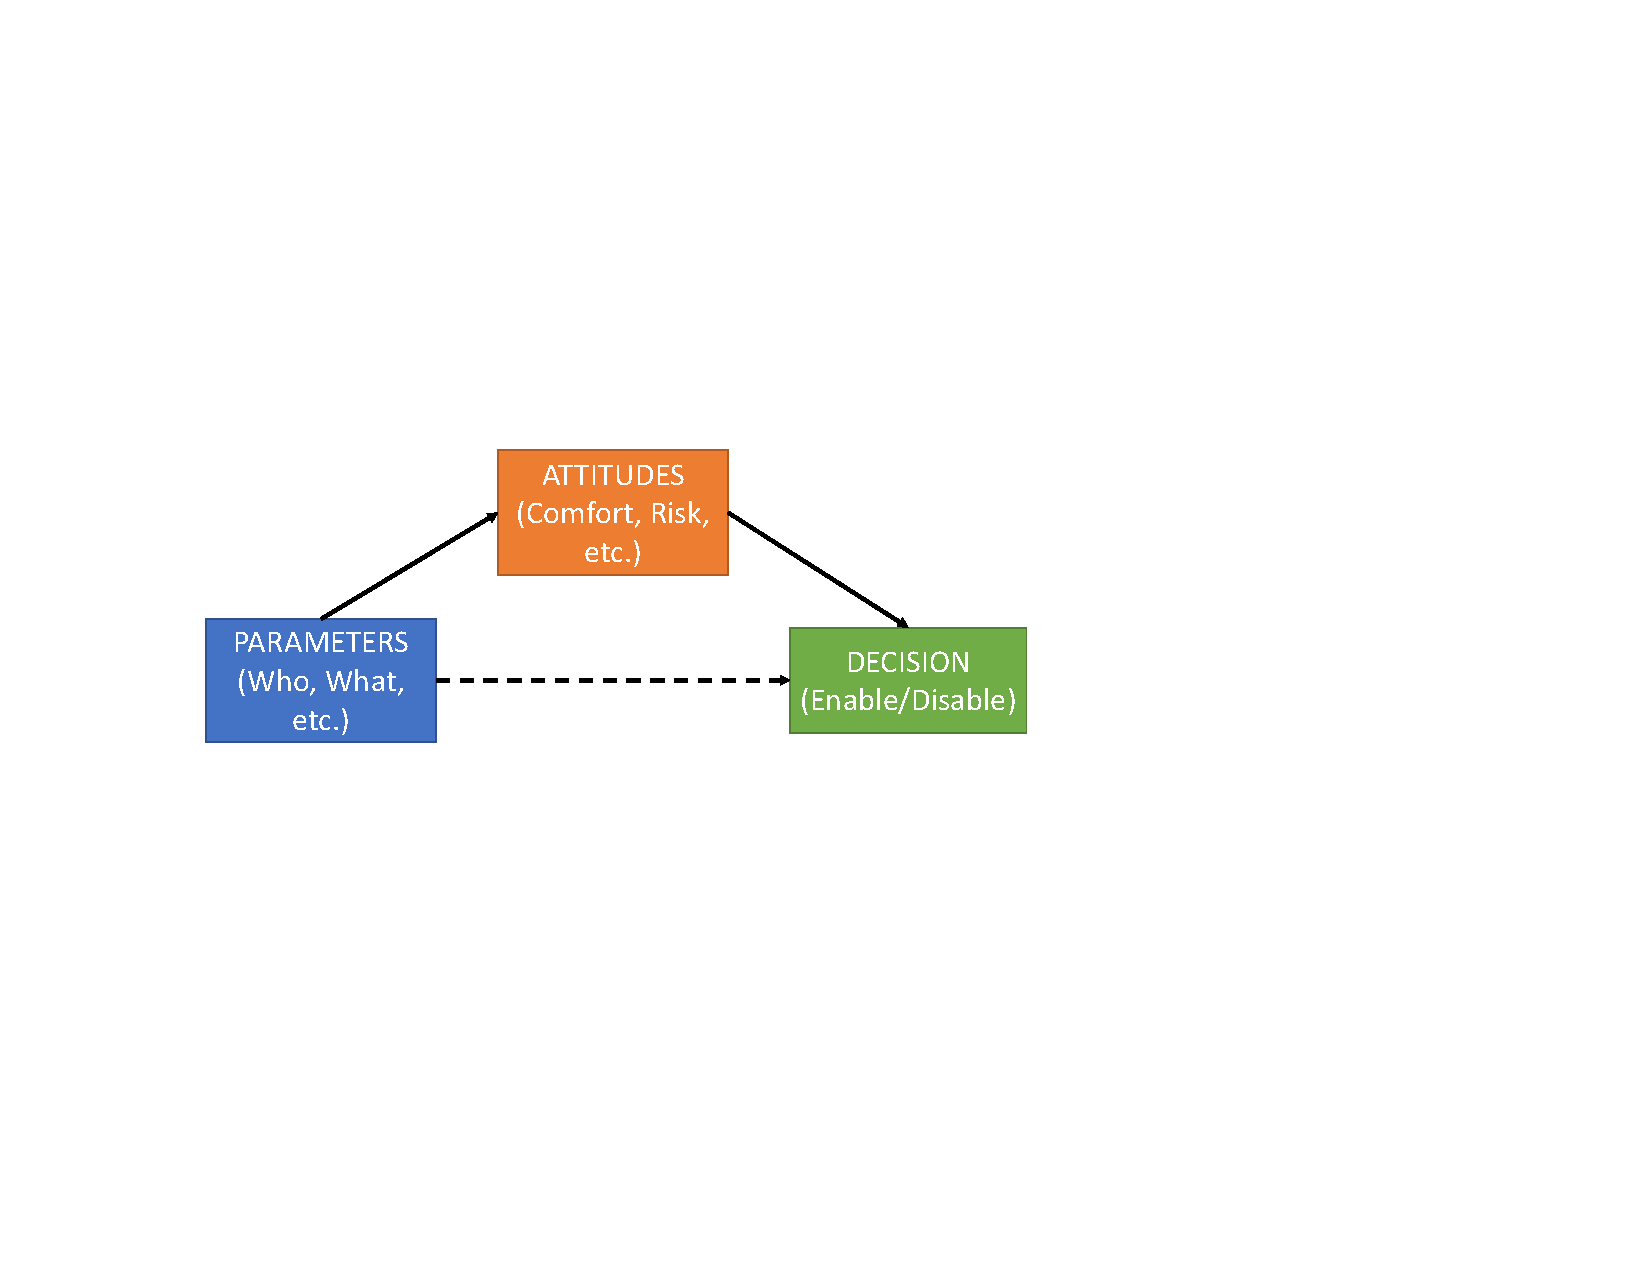
\includegraphics[width=0.75\textwidth]{figures/mediation_test.pdf}
%	\caption{Different tests conducted for mediation analysis}
%	\label{fig:mediation_test}
%\end{figure}
%
%
%Finally, we present a post-hoc analysis of differences between individual levels of the parameters on attitudes and decision.
%
%\subsection{Effect of scenario parameters on decision}
%To understand the effect of the scenario parameters on participants' allow/reject decision, we developed a \emph{generalized linear mixed effects regression} (\emph{glmer}) with a random intercept (to account for repeated measures on the same participant) and a logit link function (to account for the fact that the outcome variable is binary). We used a forward stepwise approach, where we added the strongest remaining parameter into the model into the model at each step and then comparing it using ANOVA tests against the previous model. If new parameter makes a significant improvement to the previous model, it has a significant overall effect on the outcome variable. Once all significant main effects are added to the model, two-way interaction effects are tested one by one. 
%
%Table~\ref{tab:para_decision} shows the effects of the parameters on the allow/reject decision. All parameters had a significant effect. Particularly, \textbf{Storage} had the strongest effect on participants' decisions, followed by \textbf{What}, \textbf{Who} and \textbf{Purpose} (all similar) and finally \textbf{Action}.
%
%Moreover, we find many significant interaction effects, but some of them are not substantial compared to the main effects\footnote{Very small but still significant interaction effects are a common occurrence in the analysis of large datasets.}. Substantial two-way interaction effects were observed between \textbf{Who}, \textbf{What} and \textbf{Purpose}. It should be noted that the interactions are added separately, not accumulatively. This reduces overfitting and multicollinearity.
%
%\begin{table}
%	\centering
%	\caption{Effect of scenario parameters on decision}
%	\label{tab:para_decision}
%	\begin{tabular}{ l | r | r | r }
%		\hline
%		Model &	$\chi^2$ & $df$ & $p$-value 	\\ \hline
%		$decision\sim(1 | sid)$ &		  	&	    &				\\
%		+storage &					1487.76	& 	  2 & 		$<$ .0001 	\\
%		+purpose &					206.97 &		  11 &		$<$ .0001 	\\
%		+what &				202.48 & 	  3 & 		  	$<$ .0001	\\
%		+who &			195.91 &		  7 & 		$<$ .0001 	\\
%		+action &			77.20 &		  3 & 		$<$ .0001\\\hline
%		\emph{Interactions}&			 &		  & \\\hline
%		+what:who &			138.03 &		  77 & 		$<$ .0001\\
%		+who:purpose &			87.92 &		  21 & 		$<$ .0001\\
%		+what:purpose &			68.30 &		  33 & 		.0002\\
%		\hline
%	\end{tabular}
%\end{table}
%
%\subsection{Effect of scenario parameters on attitudes}
%Test 1 of the mediation model is a test of the effect of the scenario parameters on participants' attitudes. For this we developed a separate \emph{linear mixed effects regression model} (\emph{lmer}) model with a random intercept (to account for repeated measures on the same participant) for each dependent variable (Risk, Comfort, Appropriateness, Expectedness and Usefulness), using the scenario parameters as independent variables. As in the previous section, we took a forward stepwise approach.
%
%Tables~\ref{tab:para_approp}-\ref{tab:para_exp} show the effects of the parameters on the different attitudes. All parameters had a significant effect on all attitudes. Substantial two-way interaction effects were again observed between \textbf{Who}, \textbf{What} and \textbf{Purpose}. Again, the interactions are added separately, not accumulatively.
%
%\begin{table}
%	\centering
%	\caption{Effect of scenario parameters on appropriateness}
%	\label{tab:para_approp}
%	\begin{tabular}{ l | r | r | r }
%		\hline
%		Model &	$df$ & $Chi. Sq.$ & $p$-value 	\\ \hline
%		$appropriateness\sim(1 | sid)$ &	3	  	&	    &				\\
%		+storage &					5	& 	  2346.19 & 		$<$ .0001 	\\
%		+what &					16 &		  398.63 &		$<$ .0001 	\\
%		+purpose &				19 & 	  359.98 & 		  	$<$ .0001	\\
%		+who &			26 &		  179.09 & 		$<$ .0001 	\\
%		+action &			29 &		  91.05& 		$<$ .0001\\\hline
%		\emph{Interactions}&			 &		  & \\\hline
%		+what:who &			106 &		  167.01 & 		$<$ .0001\\
%		+who:purpose &			50 &		  113.73 & 		$<$ .0001\\
%		+what:purpose &			62 &		  55.67 & 		.0081\\
%		\hline
%	\end{tabular}
%\end{table}
%
%\begin{table}
%	\centering
%	\caption{Effect of scenario parameters on comfort}
%	\label{tab:para_comfort}
%	\begin{tabular}{ l | r | r | r }
%		\hline
%		Model &	$df$ & $Chi. Sq.$ & $p$-value 	\\ \hline
%		$comfort\sim(1 | sid)$ &	3	  	&	    &				\\
%		+storage &					5	& 	  2822.57 & 		$<$ .0001 	\\
%		+what &					16 &		  391.10 &		$<$ .0001 	\\
%		+purpose &				19 & 	  381.69 & 		  	$<$ .0001	\\
%		+action &			22 &		  113.68 & 		$<$ .0001 	\\
%		+who &			29 &		  90.57& 		$<$ .0001\\\hline
%		\emph{Interactions}&			 &		  & \\\hline
%		+what:who &			106 &		  132.86 & 		$<$ .0001\\
%		+who:purpose &			50 &		  89.20 & 		$<$ .0001\\
%		+what:purpose &			62 &		  58.24 & 		 .0043\\
%		\hline
%	\end{tabular}
%\end{table}
%
%\begin{table}
%	\centering
%	\caption{Effect of scenario parameters on risk}
%	\label{tab:para_risk}
%	\begin{tabular}{ l | r | r | r }
%		\hline
%		Model &	$df$ & $Chi. Sq.$ & $p$-value 	\\ \hline
%		$risk\sim(1 | sid)$ &	3	  	&	    &				\\
%		+storage &					5	& 	  47240.72 & 		$<$ .0001 	\\
%		+purpose &					16 &		  421.08 &		$<$ .0001	\\
%		+action &				19 & 	  355.65 & 		  	$<$ .0001	\\
%		+who &			26 &		  81.35 & 		 $<$ .0001 	\\
%		+what &			29 &		  70.64 & 		 $<$ .0001\\\hline
%		\emph{Interactions}&			 &		  & \\\hline
%		+what:who &			106 &		  77.14 & 		 0.0017\\
%		+who:purpose &			50 &		  19.91 & 		$<$ .0001\\
%		+what:purpose &			62 &		  37.19 & 		0.0352\\
%		\hline
%	\end{tabular}
%\end{table}
%
%\begin{table}
%	\centering
%	\caption{Effect of scenario parameters on usefulness}
%	\label{tab:para_use}
%	\begin{tabular}{ l | r | r | r }
%		\hline
%		Model &	$df$ & $Chi. Sq.$ & $p$-value 	\\ \hline
%		$usefulness\sim(1 | sid)$ &	3	  	&	    &				\\
%		+what &					5	& 	  939.91 & 		$<$.0001 	\\
%		+storage &					12 &		  457.36 &		$<$.0001	\\
%		+purpose &				23 & 	  401.18 & 		  	$<$.0001	\\
%		+action &			26 &		  328.88 & 		 $<$.0001 	\\
%		+who &			29 &		  117.57& 		 $<$.0001\\\hline
%		\emph{Interactions}&			 &		  & \\\hline
%		+what:who &			106 &		 214.48 & 		 $<$.0001\\
%		+who:purpose &			50 &		  184.48 & 		$<$.0001\\
%		+what:purpose &			62 &		  85.39 & 		$<$.0001\\
%		\hline
%	\end{tabular}
%\end{table}
%
%\begin{table}
%	\centering
%	\caption{Effect of scenario parameters on expectedness}
%	\label{tab:para_exp}
%	\begin{tabular}{ l | r | r | r }
%		\hline
%		Model &	$df$ & $Chi. Sq.$ & $p$-value 	\\ \hline
%		$expectedness\sim(1 | sid)$ &	3	  	&	    &				\\
%		+storage &					5	& 	  841.24 & 		$<$ .0001 	\\
%		+who &					16 &		  425.92 &		$<$ .0001 	\\
%		+what &				19 & 	  422.31 & 		  	$<$ .0001	\\
%		+purpose &			22 &		  231.98 & 		$<$ .0001 	\\
%		+action &			29 &		  29.45& 		$<$ .0001\\\hline
%		\emph{Interactions}&			 &		  & \\\hline
%		+what:who &			106 &		  262.80 & 		$<$ .0001\\
%		+who:purpose &			50 &		  138.73 & 		$<$ .0001\\
%		+what:purpose &			62 &		  84.89 & 		$<$ .0001\\
%		\hline
%	\end{tabular}
%\end{table}
%
%\subsection{Effect of attitudes on decision}
%Test 2 of the mediation model is a test of the effect of participants' attitudes on their allow/reject decision. We perform this test by creating a \emph{glmer} model with a random intercept and a logit link function. Using a forward stepwise approach, we find that all attitudes except \textbf{Expectedness} have a significant effect on decision (see the top part of Table~\ref{tab:att_decision}). Specific effects are as follows:
%\begin{itemize}
%	\item Each 1-point increase in \textbf{Comfort} (measured on a 7-point scale) results in a 2.30-fold increase in the odds that the participant will allow the scenario ($p < 0.001$). 
%	\item Each 1-point increase in \textbf{Usefulness} results in a 2.09-fold increase in the odds that the participant will allow the scenario ($p < 0.001$).
%	\item Each 1-point increase in \textbf{Appropriateness} results in a 44\% increase in the odds that the participant will allow the scenario ($p < 0.001$).
%	\item Each 1-point increase in \textbf{Risk} results in a 14\% decrease in the odds that the participant will allow the scenario ($p < 0.001$).
%	\item \textbf{Expectedness} had no signficant influence on the participant's decision (p = 0.201).
%\end{itemize}
%
%
%\begin{table}
%	\centering
%	\caption{Effect of attitudes on decision; conditional effects of parameters are added subsequently}
%	\label{tab:att_decision}
%	\begin{tabular}{ l | r | r | r }
%		\hline
%		Model &	$\chi^2$ & $df$ & $p$-value 	\\ \hline
%		$decision\sim(1 | sid)$ &		  	&	    &				\\
%		+Comfort &					7934.72	& 	  1 & 		$<$ .0001 	\\
%		+Usefulness &					1249.51 &		  1 &		$<$ .0001 	\\
%		+Appropriateness &				149.15 & 	  1 & 		  	$<$ .0001	\\
%		+Risk  &			10.90 &		  1 & 		 .0009 	\\
%		+Expectedness &			1.62 &		  1 & 		 .201\\\hline
%		\emph{Adding Scenario Parameters}&			 &		  & \\\hline
%		+action &			0.332 &		  3 & 		 0.953\\
%		+what &			13.871 &		  11 & 		0.2401\\
%		+purpose &			3.60 &		  3 & 		0.3069\\
%		+storage &			14.57 &		  2 & 		0.0006\\
%		+who &			24.53 &		  7 & 		0.0009\\
%		\hline
%	\end{tabular}
%\end{table}
%
%\textcolor{blue}{The strongly significant relationship between attitudes and behavior is interesting in light of the ``privacy paradox''~\cite{norberg07}, an attitude-behavior gap that has been studied extensively by privacy researchers. Arguably, the privacy paradox is an artifact of the fact that \emph{general} privacy concerns (which are commonly high) do not match \emph{specific} behaviors (which subsequently ignore these general concerns). Since in our study attitudes and behaviors are measured at the same contextual level, their relationship is much stronger than in other studies. This may explain why we do not find an attitude-behavior gap.}
%
%
%\subsection{Mediation analysis}
%With tests 1 and 2 of our mediation analysis confirmed, we conduct test 3 by adding the scenario parameters to the \emph{glmer} of participants' decisions on their attitudes. The bottom half of Table~\ref{tab:att_decision} shows these conditional effects of the significant scenario parameters on participants' allow/reject decision, controlling for their attitudes. \textbf{Action}, \textbf{What} and \textbf{Purpose} are no longer significant in this model, suggesting that these effects are \emph{fully mediated} by participants' attitudes. \textbf{Storage} and \textbf{Who} are still significant, but their conditional effects are smaller than their marginal effects on decision (without controlling for attitude, see Table~\ref{tab:para_decision}). Their $chi^2$s are reduced drastically by 98\% and 87\%, respectively. Overall, there was a substantial mediation effect. Figure~\ref{fig:mediation_model} shows the final model mediation model.
%
%\begin{figure}
%	\centering
%	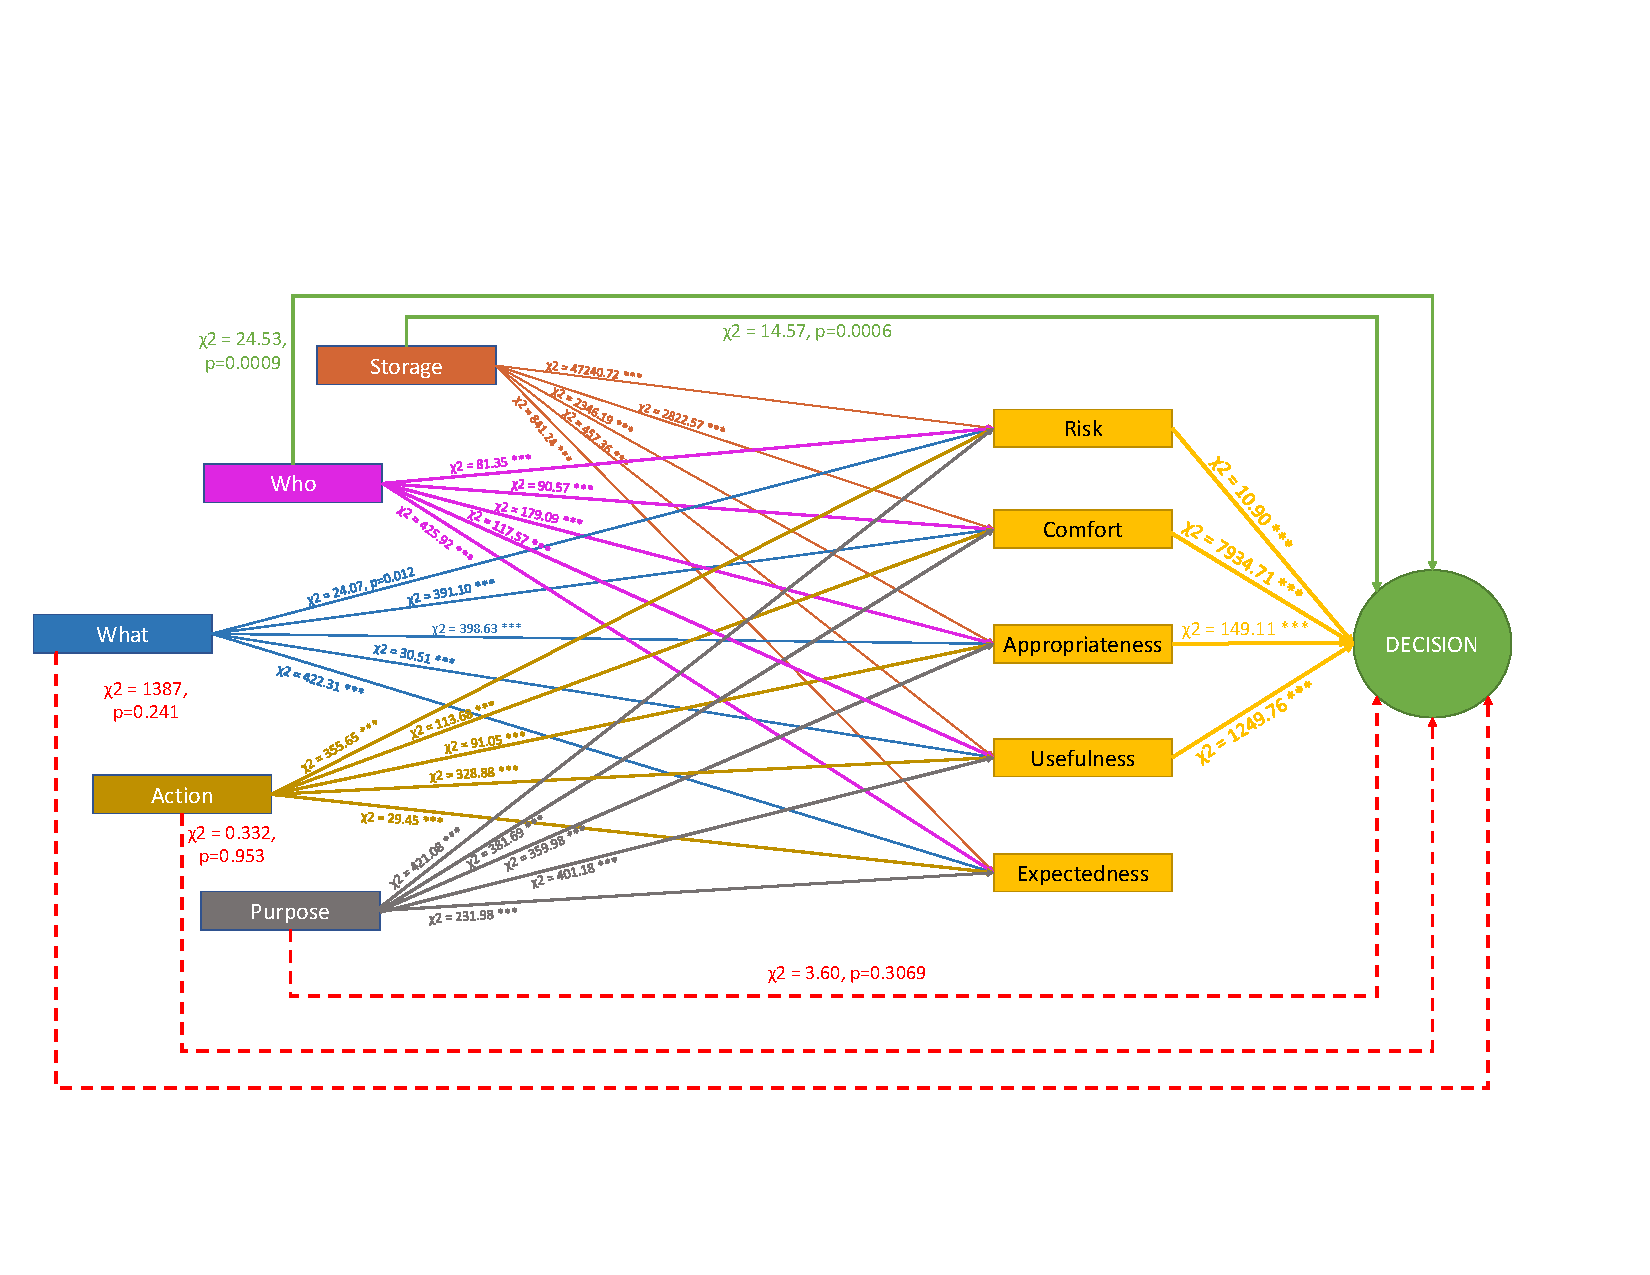
\includegraphics[width=0.95\textwidth]{figures/mediation.pdf}
%	\caption{Final mediation model.}
%	\label{fig:mediation_model}
%\end{figure}
%
%
%\subsection{Post-hoc Results}
%To understand the effects of different values of each parameter on participants' various attitudes and their allow/reject decision, we conducted \textcolor{blue}{post-hoc tests using Tukey's method to adjust $p$-values to account for familywise error.} This subsection highlights the key insights from these tests. For an overview of the differences between parameter values, the reader is invited to visually inspect them by referring to Figures~\ref{fig:storage_post}-\ref{fig:what_post} in the Appendix.
%
%\textbf{Storage}: Participants perceive more risk ($d$ range $= [0.568, 1.707]$, all $p$s $< .001$), are less comfortable ($d$ range $= [0.538, 1.741]$, all $p$s $< .001$) and find it inappropriate ($d$ range  $=  [0.436, 1.550]$, all $p$s $< .001$) when their information is shared to `third parties' or `stored on a remote server' as compared to when it is stored `locally'. Participants also found it less useful to share their information with third parties as compared to storing it locally or on a remote server ($d$ range $= [0.28, 1.02]$,  $p < .001$). Interestingly, participants expected it less that the information is stored locally rather than stored on remote server or shared to third parties ($d$ range $= [0.212, 0.894]$, all $p$s $< .001$). Finally, the odds of enabling a feature when information is stored locally were 1.96 times higher than when information is stored on a remote server ($p < .001$) and 8.36 times higher than when information is shared with third parties ($p < .001$).
%
%\textbf{Action}: Participants were less comfortable ($d$ range $= [0.158, 0.348]$, all $p$s $< .001$) and found it more risky ($d$ range $= [0.145, 0.262]$, all $p$s $< .001$) when their information is used to give them recommendations instead of optimizing services or giving them insight into their behavior. Sharing information was also found less useful ($d = 0.293$, $p < .001$) and less appropriate ($d = 0.256$, $p < .001$) for recommendation purposes as opposed to when the scenario did not specify any purpose. Participants also expected it less ($d = 0.123$, $p = .0021$) when their information was being shared for recommendation purposes as opposed to when the scenario did not specify any purpose. Finally, the odds of enabling a feature for recommendation purposes were 1.53 times lower as opposed to when the scenario did not specify any purpose ($p < .001$). Additionally, the odds of enabling a feature for optimization purposes were 1.65 times higher than for recommendation purposes ($p < .001$) and 1.26 times higher than for giving behavioral insights ($p < .001$). 
%
%\textbf{Purpose}: Participants found it inappropriate ($d$ range $= [0.343, 0.411]$, all $p$s $< .001$) when information is collected for the purpose of detecting their presence in the house as compared to the purposes of automating operations or giving timely alerts, and it was even more inappropriate to collect information for the purpose of detecting their location in the house ($d$ range $= [0.163, 0.574]$, all $p$s $< .001$). Participants also found it more risky when information is used for location detection as compared to presence detection ($d = 0.598$, $p < .001$), but they found it less risky to share information for the purpose of giving timely alerts or for automating operations ($d$ range  $= [0.550, 0.601]$, $p$ range $= [0.002, 0.004]$). Participants also found it more useful when information is collected for the purpose of providing alerts ($d = 0.558$, $p < .001$) or for automating operations ($d = 0.603$, $p < .001$) compared to the purpose of detecting their location in the house. Finally, the odds of enabling a feature were 1.29 times higher for detecting their presence in house than for detecting their location ($p = 0.0002$). Moreover, the odds of enabling a feature for the purpose of giving timely alerts and automating operations were 1.59 ($p < .001$) and 1.65 ($p < .001$) times higher respectively. 
%
%\textbf{Who}: Participants expected it more that their smart security systems will access information as compared to other devices such as their smart HVAC, TV, alarm and washing machine ($d$ range $=  [0.267, 0.618]$, all $p$s $< .001$). Users perceived data access by their security systems as more useful compared other devices like their smart refrigerator, washing machine, TV and HVAC ($d$ range $= [0.386, 0.627]$, all $p$s $< .001$). Participants were more comfortable ($d = 0.196$, $p = .002$) and found it less risky ($d = 0.263$, $p < .001$) for their security systems to access collected data as compared to their smart lighting systems. Also, participants were more comfortable ($d$ range $=  [0.173, 0.356]$, all $p$s $< .05$) and found it less risky ($d$ range $= [0.256, 0.338]$, all $p$s $< .05$) for their lighting systems to access collected data compared to their smart assistant, TV and alarm clock. Finally, the odds of users enabling access to their smart security system were higher than to their smart refrigerator and washing machine by 1.8 times($p < .001$), their smart TV by 1.7 times ($p < .001$) and their smart alarm clock by 1.6 times ($p < .001$). We found similar results for participants' smart assistant which had odds higher than their smart TV (1.76 times higher,  $p < .001$), their smart alarm clock (1.68 times higher,  $p < .001$), their smart washing machine (1.90 times higher,  $p < .001$) and their smart refrigerator (1.85 times higher,  $p < .001$).
%
%\textbf{What}: This parameter had twelve different values and there were numerous combinations that were significant when we checked the post-hoc effects. We limit our discussion to the differences between the `Smart Assistant' and the other values of this parameter, because these specific differences are consistently significant. The reader is invited to inspect Figure~\ref{fig:who_post} in the Appendix for other differences. Participants found it more appropriate ($d$ range $= [0.213, 0.756]$, all $p$s $< .001$) and useful ($d$ range $= [0.365, 0.683]$, all $p$s $< .01$) when information collected by their smart assistant was being accessed as compared to other devices like cameras or microphones. The participants also found it less risky ($d$ range $= [0.385, 0.759]$, all $p$s $< .05$) and were more comfortable ($d$ range $= [0.430,0.821]$, all $p$s $< .01$) to grant access to information collected by their smart assistant than their camera or microphone. Participants also expected more to share information collected by their smart assistant as compared to other devices such as cameras ($d = 0.62$, $p < .01$), microphones ($d = 0.39$, $p < .01$), or their smart alarm clock ($d = 0.21$, $p = .027$). The odds of giving access to information collected by their smart assistant were higher than for cameras by 2.7 times ($p < .001$), microphones by 1.8 times ($p < .001$), their Smart TV by 1.15 times ($p < .001$) and their smart washing machine by 1.8 times ($p < .001$).

\section{Statistical Analysis}\label{sec:statAlys2}
Our statistical analysis shows that unlike results from~\cite{bahiratiui2018}, all parameters had a significant effect. Particularly, where the information is stored and if/how it is shared with third parties (`Storage' parameter) has the strongest impact on users' decision, followed by `What', `Who' and `Purpose' (all similar) and finally `Action'. Moreover, substantial two-way interaction effects were observed between `Who', `What', and `Purpose', which suggest that when users decide on one parameter, they inherently take another parameter into account. Based on these results, we designed an interface, which separated `Device/Sensor Management' and `Data Storage \& Usage', for users to manually change their privacy settings. 

We also analyze the effects of defaults and framing. As outlined in section \ref{sec:questions}, the framing and default of the Decision question in our study were manipulated between-subjects at three levels each: positive, negative, or neutral framing; combined with a positive, negative, or no default. The analysis shows that defaults and framing have direct effects on disclosure: Participants in the negative default condition are less likely to enable the functionality, while participants in the positive default condition are more likely to enable the scenario (a traditional default effect). Likewise, participants in the negative framing condition are more likely to enable the functionality (a loss aversion effect).

Moreover, there are interaction effects between defaults/framing and attitudes on disclosure: the effects of attitudes are generally weaker in the positive and negative default conditions than in the no default condition, and they are also weaker in the negative framing condition.

Importantly, there are no interaction effects between defaults/framing and parameters on attitude or disclosure. Hence, the main findings in this section regarding the structure and relative importance of the effects of parameters remain the same, regardless of the effects of defaults and framing.

%
%\subsection{Discussion}
%
%In Chapter~\ref{chapter:Acceptability}, we found that privacy risk is an increasingly important barrier to the adoption of household IoT devices. Interestingly, though, in our study Comfort, Usefulness and Appropriateness had a stronger effect on users' allow/reject decisions than Risk. This suggests that IoT devices with a trust-inspiring design, a strong value proposition, and a clear explanation of the appropriateness of their data collection practices can overcome initial perceptions of privacy risk.
%
%The trade-off between Comfort, Usefulness and Appropriateness embodies an interesting trade-off: Usefulness is associated with the utility of a feature, whereas Appropriateness is a contextual evaluation (is this acceptable given the \emph{situation}?) and Comfort is a self-relevant evaluation (is this acceptable for \emph{me}?).
%
%The interaction between \textbf{What}, \textbf{Who}, and \textbf{Purpose} also suggests that users make context-relevant evaluations: scenarios are not accepted based on the sum of their components; rather, certain combinations of devices and purposes are more acceptable than others. While this is outside the scope of the current paper, future work could look into this context-dependency to find specific synergistic combinations. 
%
%The \textbf{Storage} parameter had the most significant influence on participants' decision and all attitudes, but most prominently on Risk. ($chi^2 = 47240.72$,  $p < .001$). This indicates that users' risk perceptions are mostly dependent on the way household IoT systems store and share their data. Household IoT device manufacturers who want to reduce risk perceptions may want to opt for storing all data locally instead of on a remote server (something users are actually more likely to expect). %This is particularly true for smart assistants, whose collected data is least likely to be shared with other devices anyway. %Interestingly, while most smart assistants collect their data via a microphone or camera, users are less comfortable sharing the data collected data by their smart assistant than the data collected by microphone or camera sensors.
%
%Finally, the \textbf{Action} parameter had the least significant influence. Arguably, once users allow information to be collected, they care less about how exactly it is being used (or possibly, they do not expect to be able to control how it is being used).
%
%\subsubsection{Designing for IoT by prioritizing parameters}
%The results of our analyses uncover an intuitive reality about our household IoT scenarios, namely, they consist of two somewhat separate parts: On the one hand, there is a device (\textbf{Who}) that accesses information collected by another device (\textbf{what}), for a purpose certain \textbf{Purpose}. At the same time, this the collected information may be stored somewhere (\textbf{Storage}) and some \textbf{Action} may be performed on it. 
%
%For the first aspect, we observed substantial interaction effects between all the three parameters, indicating that users want to make intricate decisions about what information is going where and for what purposes. Specifically, Unlike Bahirat et. al. ~\cite{bahiratiui2018}, we cannot use an interface with a separate `layer' for each parameter; the interaction effects suggest that when uses decide on one parameter, they inherently take another parameter into account. Therefore the settings interface for device/sensor management should show all three parameters at the same time to allow users to make these decisions.
%
%For the second aspect, data storage had a very strong impact, while the action had the weakest impact. Additionally, there were no interactions between these two parameters, nor did they interact with any of the other parameters. This suggests that data storage and use can be separated in our privacy-setting interface. 

\section{Privacy-Setting Prototype Design}\label{sec:design_stat}

Our dataset presents a simplified version of possible scenarios one might encounter in routine usage of smart home technology. Still it is a daunting task to design an interface, even for these simplified scenarios: We want to enable users to navigate their information collection and sharing preferences across 12 different sources (\emph{What}), 7 different devices trying to access this information (\emph{Who}) for 4 different \emph{Purposes}. Additionally, this information is being stored/shared in 3 ways (\emph{Storage}) and being used for 4 different longer-term (\emph{Actions}). 

Based on our statistical analysis in~\ref{sec:statAlys2}, we developed an intuitive interface that gives users manual control over their privacy settings. We split our settings interface into two separate sections: `Device/Sensor Management' and `Data Storage \& Use'. The landing page of our design (screen 1 in Figure~\ref{fig:interface2}) gives users access to these two sections. The former section is based on \emph{Who}, \emph{What} and \emph{Purpose} and allows users to ``Manage device access to data collected in your home'' (screen 2-3). The latter section is based on \emph{Storage} and \emph{Action}, and allows users to ``Manage the storage and long-term use of data collected in your home'' (screen 4). Both sections are explained in more detail below.

\begin{figure}
	\centering
	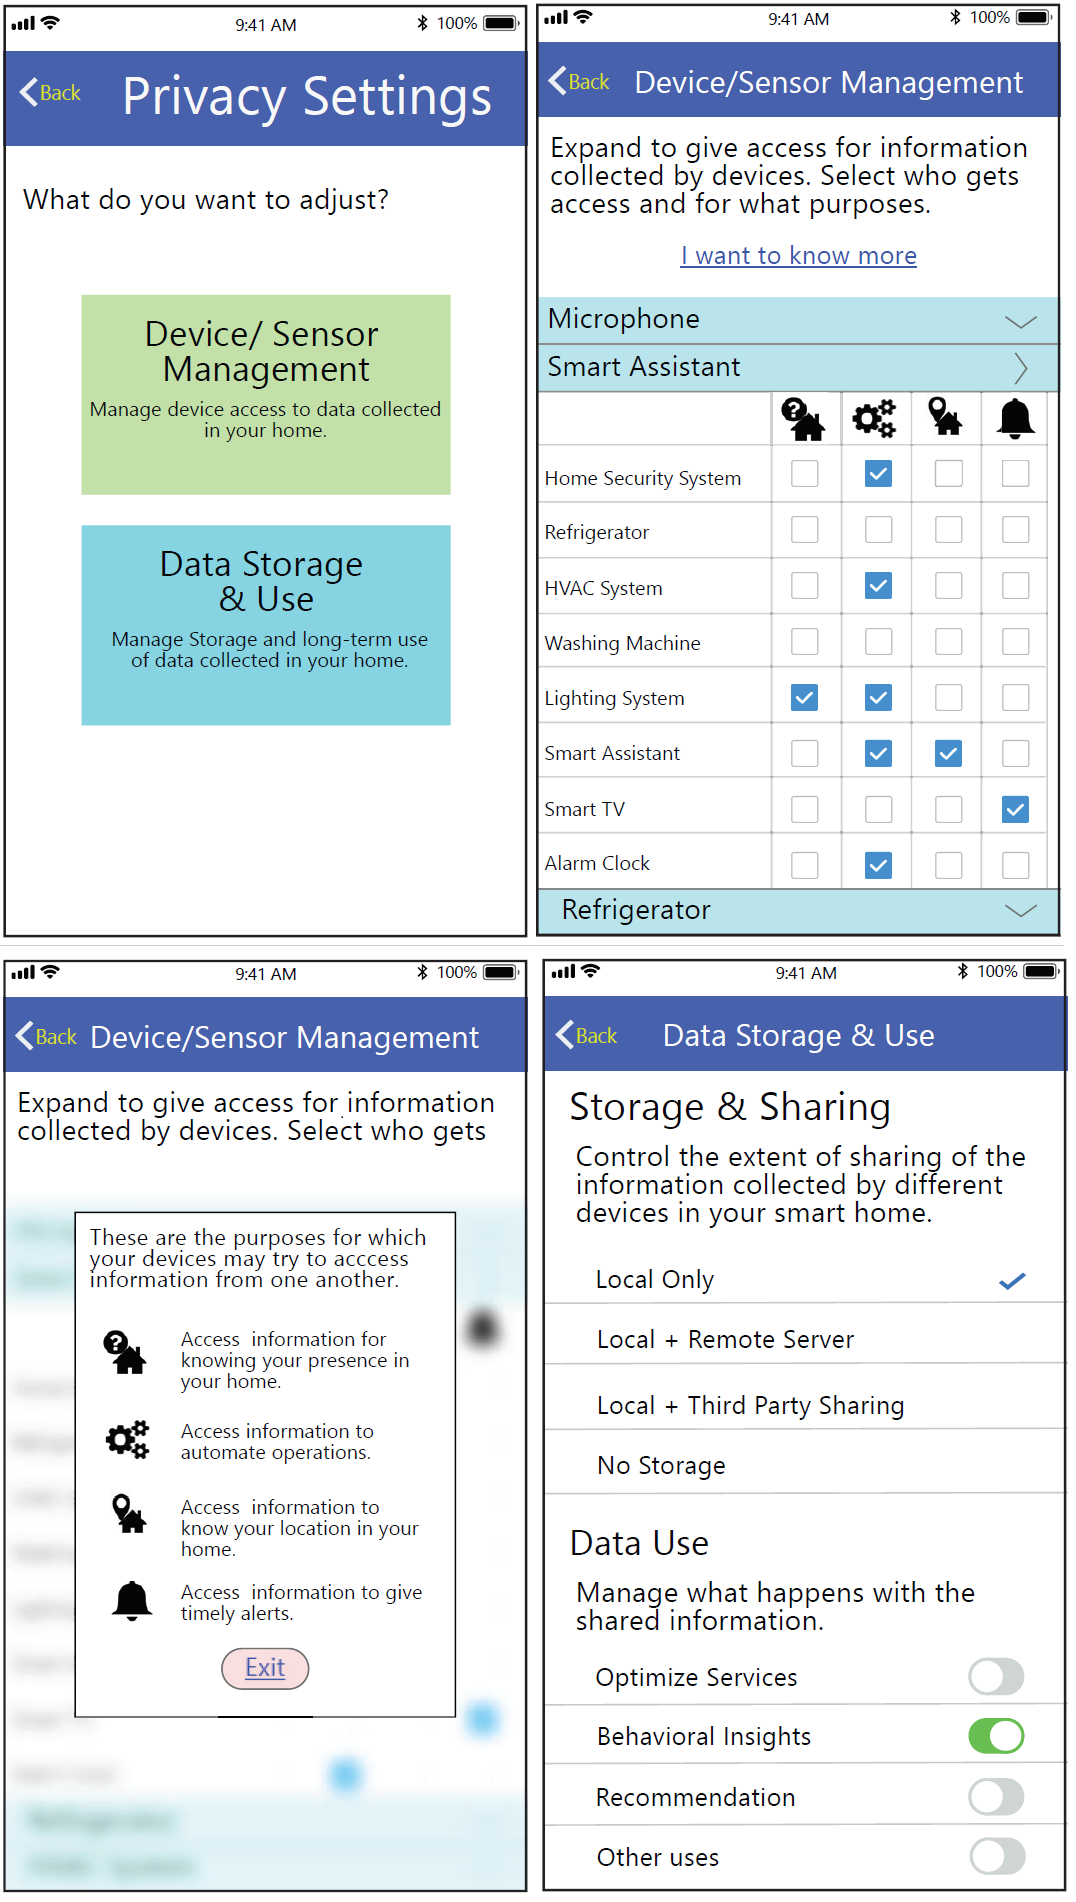
\includegraphics[width=0.7\textwidth]{figures/interface_new.png}
	\caption{Screen 1 (top left) is the landing page of our manual settings interface, screen 2 (top right) is the Device/Sensor Management page, screen 3 (bottom left) shows the explanation when you click on ``I want to learn more'', and screen 4 (bottom right) is the Data Storage \& Use page.}
	\label{fig:interface2}
\end{figure}

\textbf{Device/Sensor Management:} This screen (Figure~\ref{fig:interface2}, screen 2) allows users to control the \emph{Purposes} for which each device (\emph{Who}) is allowed to access data collected by itself, other devices, and the smart home sensors installed around the house (\emph{What}). This screen has a collapsible list of data-collecting devices and sensors (\emph{What}). For each device/sensor, the user can choose what devices can access the collected data (\emph{Who}; in rows), and what it may use that data for (\emph{Purpose}; in columns).

In the example of Figure~\ref{fig:interface2}, the user does not give the `Refrigerator' access to information collected by the `Smart Assistant' for any of the four purposes, while they give the `Smart TV' access to this data for the purpose of giving `timely alerts'. In this example the `Smart Assistant' is allowed to use its own data to `automate operations' and to `know your location in your home'.

Showing \emph{Who}, \emph{What} and \emph{Purpose} at the same time allows users to enable/disable specific combinations of settings---the significant interaction effects between these parameters suggest that this is a necessity. The icons for the \emph{Purpose} requirement allow this settings grid to fit on a smartphone or in-home control panel. We expect that users will quickly learn the meaning of these icons, but they can always click on `I want to know more' to learn their meaning (see Figure~\ref{fig:interface2}, screen 3). 

%If users want to further provide access for specific purpose, then they can click on `More'. Once users tap on `More' they are navigated to Screen-1 of the interface where they can see the different levels of `Purpose' parameter. By showing different levels of `Who' and `What' parameters on Screen-2, we account for the interaction effects between them, the user can now see both the levels at a time thereby making a decision on the grounds of both of these parameters. In Screen-1 we also account for interactions between `Who-What' and `Purpose' because at the bottom of this Screen, users see the flow of information across different device of the former parameters.

%Although, `Purpose' seems to be slightly more important parameter as compared to `Who' and `What', while designing, we envisaged that the interaction effects between `Who' and `What' play a more dominant role and showing different devices involved in the latter parameters would help users gain a quicker grasp over the flow of information in the system.

\textbf{Data Storage \& Use:} This screen (Figure~\ref{fig:interface2}, screen 4) allows users to control how their data is stored and shared (\emph{Storage}), as well as how stored data is used (\emph{Action}). These settings are independent from each other and from the Device/Sensor Management settings. 

For `Storage \& Sharing', users can choose to turn storage off altogether, store data locally, store data both locally and on a remote server, or store data locally and on a remote server \emph{and} allow the app to share the data with third parties. Note that the options for \emph{Storage} are presented as ordered, mutually exclusive settings. Our scenarios did not present them as such (i.e., participants were free to reject local storage but allow remote storage). However, the \emph{Storage} parameter showed a very clear separation of levels%(see Figure~\ref{fig:storage_post} in the Appendix)
, so this presentation is justified. For `Data Use', the users can choose to enable/disable the use of the collected data for various secondary purposes: behavioral insights, recommendations, service optimization, and/or other purposes.

In the subsequent sections we describe the results from our machine learning analysis and further explain how these results impact the designs presented in this section. For this purpose, Section~\ref{sec:design_ml} revisits the interface designs presented here.

\section{Predicting users' behaviors (original work)}\label{sec:predict}
In this section we predict participants' \textit{enable}/\textit{disable} decision using machine learning methods. Similarly, we do not attempt to find the best possible solution; instead we make a conscious trade-off between parsimony and prediction accuracy. Accuracy is important to ensure that users' privacy preferences are accurately captured and/or need only few manual adjustments. Parsimony, on the other hand, prevents overfitting and promotes fairness: we noticed that more complex models tended to increase overall accuracy by predicting a few users' preferences more accurately, with no effect on other users. Parsimony also makes the associated default setting easier to understand for the user.

%Our prediction target is the participants' decision to \textit{enable} or \textit{disable} the data collection described in each scenario. The scenario parameters serve as input attributes. These are nominal variables, making decision tree algorithms such as ID3 and J48 a suitable prediction approach. Unlike ID3, J48 uses gain ratio as the root node selection metric, which is not biased towards input attributes with many values. Moreover, by using J48 decision trees, the amount of pruning for the model can be easily manipulated to investigate the trade-off between the accuracy and parsimony. We therefore use J48 throughout our analysis.

Our prediction target is the participants' decision to \textit{enable} or \textit{disable} the data collection described in each scenario. The scenario parameters serve as input attributes. Using Java and Weka's Java library~\cite{witten2016data} for modeling and evaluation, we implement progressively sophisticated methods for predicting participants' decisions. After discussing naive (enable/disable all) solutions and One Rule Prediction, we first present a cross-validated tree learning solution that results in a single ``smart default'' setting that is the same for everyone. Subsequently, we discuss three different procedures that create a number of ``smart profiles'' by clustering the participants and creating a separate cross-validated tree for each cluster. For each procedure, we try various numbers of clusters and pruning parameters. The solutions with the most parsimonious trees and the highest accuracies of each approach are reported in Table~\ref{tab:comp_approach2}; more detailed results of the parsimony/accuracy trade-off are presented in Figures~\ref{fig:smart_default_optimal}, \ref{fig:attitudesum}, \ref{fig:conglosum} and \ref{fig:fitsum} throughout the paper, and combined in Figure~\ref{fig:summary}.

\newcommand{\specialcell}[2][c]{%
	\begin{tabular}[#1]{@{}c@{}}#2\end{tabular}}

\begin{table}
	\centering
	\caption{Comparison of clustering approaches (highest parsimony and highest accuracy)}
	\label{tab:comp_approach2}
	\begin{tabular}{l|c|c|c|c}
		\hline
		Approach & \specialcell{Inital \\ clusters} & \specialcell{Final \# of \\ profiles} & \specialcell{Complexity \\ (avg. tree size/profile)} & Accuracy \\ \hline
		Naive (enable all) & 1 & 1 & 1 & 46.74\% \\
		Naive (disable all) & 1 & 1 & 1 & 53.26\% \\ \hline
		One Rule (Fig.~\ref{fig:oneR}) & 1 & 1 & 3 & 61.39\% \\ \hline
		\multirow{2}{8em}{Overall (Fig.~\ref{fig:smart_default_optimal})} 
		& 1 & 1 & 8 & 63.32\% \\ 
		& 1 & 1 & 264 & 63.76\% \\ \hline 
		\multirow{6}{8em}{Attitude-based clustering (Fig.~\ref{fig:attitudesum})}
		& 2 & 2 & 2 & 69.44\% \\
		& 2 & 2 & 121.5 & 72.66\% \\ \cdashline{2-5}[.5pt/1pt]
		& 3 & 3 & 2.67 & 72.19\% \\
		& 3 & 3 & 26.67 & 73.47\% \\ \cdashline{2-5}[.5pt/1pt]
		& 5 & 4 & 3 & 72.61\% \\ 
		& 5 & 4 & 26 & 73.56\% \\ \hline
		\multirow{3}{8em}{Agglomerative clustering (Fig.~\ref{fig:conglosum})} & 1133 & 4 & 2 & 79.4\% \\ 
		& 1133 & 5 & 2.4 & 80.35\% \\ 
		& 1133 & 6 & 3.17 & 80.60\% \\ \hline
		\multirow{8}{7.5em}{Fit-based clustering (Fig.~\ref{fig:fitsum})} 
		& 2 & 2 & 2 & 74.43\% \\
		& 2 & 2 & 151.5 & 76.72\% \\ \cdashline{2-5}[.5pt/1pt]
		& 3 & 3 & 7 & 79.80\% \\
		& 3 & 3 & 65.33 & 80.81\% \\ \cdashline{2-5}[.5pt/1pt]
		& 4 & 4 & 9.25 & 81.88\% \\
		& 4 & 4 & 58.25 & 82.41\% \\ \cdashline{2-5}[.5pt/1pt]
		& 5 & 5 & 4.2 & 82.92\% \\
		& 5 & 5 & 51.4 & 83.35\% \\ \hline
	\end{tabular}
\end{table}

\subsection{Naive Prediction Model}
We start with the naive or ``information-less" predictions. Compared to our previous work~\cite{bahiratiui2018}, our current dataset shows that it is even less amenable to a `simple' default setting: it contains 6335 \emph{enable} cases and 7241 \emph{disable} cases, which means that predicting \textit{enable} for every setting gives us a 46.74\% prediction accuracy, while making a \textit{disable} prediction for every setting gives us an accuracy of 53.26\%. In other words, if we disable all information collection by default, only 53.26\% users will on average be satisfied with this default settings. Moreover, such a default setting disallows any `smart home' functionality by default---arguably not a solution the producers of smart appliances can get behind.

\subsection{One Rule Prediction}
Next, we use a ``\textit{One Rule}" (OneR) algorithm to predict users' decision using the simplest prediction model possible. OneR is a very simple but often surprisingly effective learning algorithm~\cite{Holte1993}. It creates a frequency table for each predictor against the target, and then find the best predictor with the smallest total error based on the frequencies.

As shown in Figure~\ref{fig:oneR}, the OneR model predicts users' decision solely based on the \textbf{Storage} parameter with an accuracy of 61.39\%.  Based on this model, if we enable all information-sharing \emph{except} with third parties, we will on average satisfy 61.39\% of users' preferences---a 15.3\% improvement\footnote{61.39 / 53.26 = 1.153} over the naive ``disable all'' default. Note, though, that this default setting is overly permissive, with 3262 false positive predictions (see Table~\ref{tab:oner_confusion_matrix}).

\begin{figure}
	\centering
	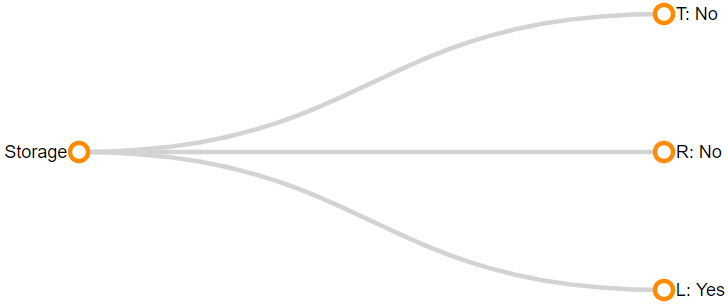
\includegraphics[width=0.6\textwidth]{figures/oneR.png}
	\caption{A ``smart default'' setting based on the ``One Rule" algorithm (4 nodes, accuracy: 61.39\%). Parameter value abbreviations correspond to the ``code'' column in Table~\ref{tab:parameter2}.}
	\label{fig:oneR}
\end{figure}


\begin{table}
	\centering
	\caption{Confusion matrix for the One Rule prediction}
	\label{tab:oner_confusion_matrix}
	\begin{tabular}{c|c|c|c} \hline
		Observed &\multicolumn{2}{c|}{Prediction} & Total\\ \cline{2-3}
		& Enable     & Disable       &  \\ \hline
		Enable   & 5085 (TP) & 1270 (FN)  & 6355   \\ \hline
		Disable    & 3262 (FP)  & 3979 (TN) & 7241  \\ \hline
		Total & 7192     & 6404     & 13596  \\ \hline
	\end{tabular}
\end{table}

\subsection{Overall Prediction}
Moving beyond a single parameter, we create a ``smart default'' setting by predicting the \textit{enable}/\textit{disable} decision with all scenario parameters using the J48 decision tree algorithm.
The resulting tree has an accuracy of 63.76\%. As shown in Figure~\ref{fig:smart_default}, this model predicts users' decision on \textbf{Storage} first. It predicts \textit{disable} for every scenarios with collected data stored on a remote server and shared with third party. For scenarios that store collected data on remote server without sharing, the default settings will depend on the `purpose' of information sharing. There is a further drill down based on `who' and `what'. For scenarios that store collected data locally, the default settings will depend on the `what'. There is a further drill down based on `who', `what', and `action'. With this default setting, users would on average be satisfied with 63.76\% of these settings---a 19.7\% improvement over the naive ``disable all" default. 

\begin{figure}
	\centering
	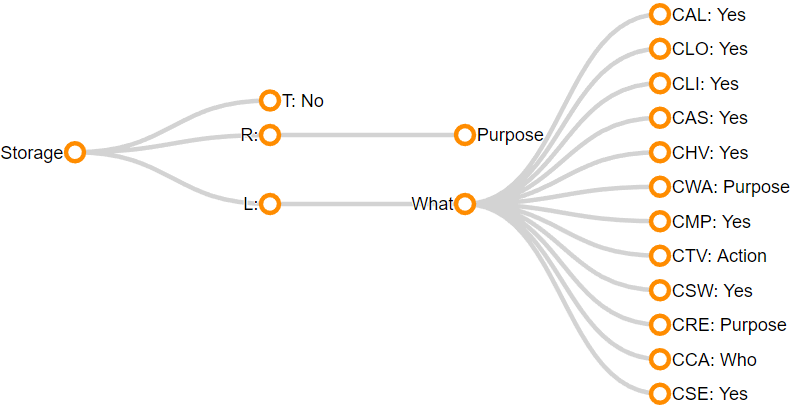
\includegraphics[width=0.7\textwidth]{figures/smartdefault025.png}
	\caption{A ``smart default'' setting with 264 nodes (accuracy: 63.76\%). Parameter value abbreviations correspond to the ``code'' column in Table~\ref{tab:parameter2}.}
	\label{fig:smart_default}
\end{figure}

On the downside, this ``smart default'' setting is quite complex---the ``smart default'' in our previous work~\cite{bahiratiui2018} contained only 49 nodes, whereas the ``smart default'' for our current dataset has 264 nodes. Compared to \textit{One Rule} algorithm, which only has 4 nodes in its decision tree and is thus much easier to explain, the accuracy improvement of Smart Default is only 3.8\%. This highlights the trade-off between parsimony and prediction accuracy that we have to make when developing ``smart default'' settings. On the upside, though, the prediction of the J48 decision tree algorithm is more balanced, with a roughly equal number of false positives and false negatives (see Table~\ref{tab:confusion_matrix2}).


\begin{table}
	\centering
	\caption{Confusion matrix for the overall prediction}
	\label{tab:confusion_matrix2}
	\begin{tabular}{c|c|c|c} \hline
		Observed &\multicolumn{2}{c|}{Prediction} & Total\\ \cline{2-3}
		& Enable     & Disable       &  \\ \hline
		Enable   & 4753 (TP) & 2488 (FN)  & 7241   \\ \hline
		Disable    & 2439 (FP)  & 3916 (TN) & 6355  \\ \hline
		Total & 7192     & 6404     & 13596  \\ \hline
	\end{tabular}
\end{table}

To better understand the parsimony/accuracy trade-off, we vary the degree of model pruning to investigate the effect of increasing the parsimony (i.e., more trimming) on the accuracy of the resulting ``smart default'' setting. The parameter used to alter the amount of post-pruning performed on the J48 decision trees is called Confidence Factor ($CF$) in Weka, and lowering the Confidence Factor will incur more pruning. We tested the J48 classifier with a Confidence Factor ranging from 0.01 to 0.25 (the default setting in Weka) with an increments of 0.01.

Figure~\ref{fig:smart_default_cf} displays the accuracy and the size of the decision tree as a function of the Confidence Factor. The X-axis represents the Confidence Factor; the left Y-axis and the orange line represent the accuracy of the smart default setting; the right Y-axis and the dotted blue line represent the size of the decision tree for that setting. The highest accuracy, 63.75\%, is achieved with the 264-node decision tree produced by $CF = 0.25$. The lowest accuracy, 62.9\%, is achieved with the 44-node decision tree produced by $CF = 0.19$. When $CF \leq 0.16$, the decision tree contains only 8 nodes. The 8-node profile with the highest accuracy is produced by $CF = 0.10$ with an accuracy of 63.32\%.

\begin{figure}
	\centering
	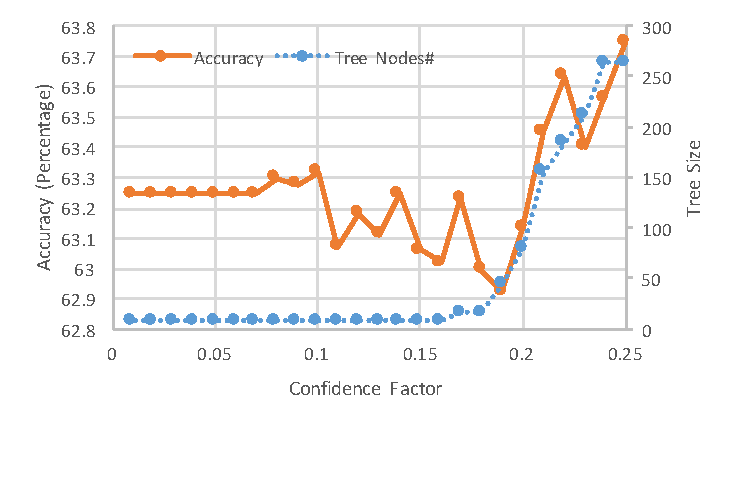
\includegraphics[width=0.65\textwidth]{figures/smart_default_cf.pdf}
	\caption{Accuracy and parsimony (tree size) of the smart default change as a function of Confidence Factor}
	\label{fig:smart_default_cf}
\end{figure}

Figure~\ref{fig:smart_default_optimal} summarizes accuracy as a function of parsimony. The X-axis represents the number number of nodes in the decision tree (more = lower parsimony); the Y-axis represents the accuracy of the decision tree. The figure shows the most accurate J48 solution for any given tree size, and includes the One Rule and Naive predictions for comparison. Reducing the tree from 264 to 8 nodes incurs a negligible 0.67\% reduction in accuracy. This decision tree is shown in Figure~\ref{fig:smart_default_new}, and is still 3.1\% better than the One Rule prediction model and 18.9\% better than the naive ``disable all" default. This more parsimonious ``smart default'' setting  can easily be explained to users as follows: 
\begin{itemize}
	\item All sharing with third parties will be disabled by default. 
	\item Remote storage is allowed for automation and alerts, but not for detecting your presence or location in the house. 
	\item Local storage is allowed for all purposes.
\end{itemize}


\begin{figure}
	\centering
	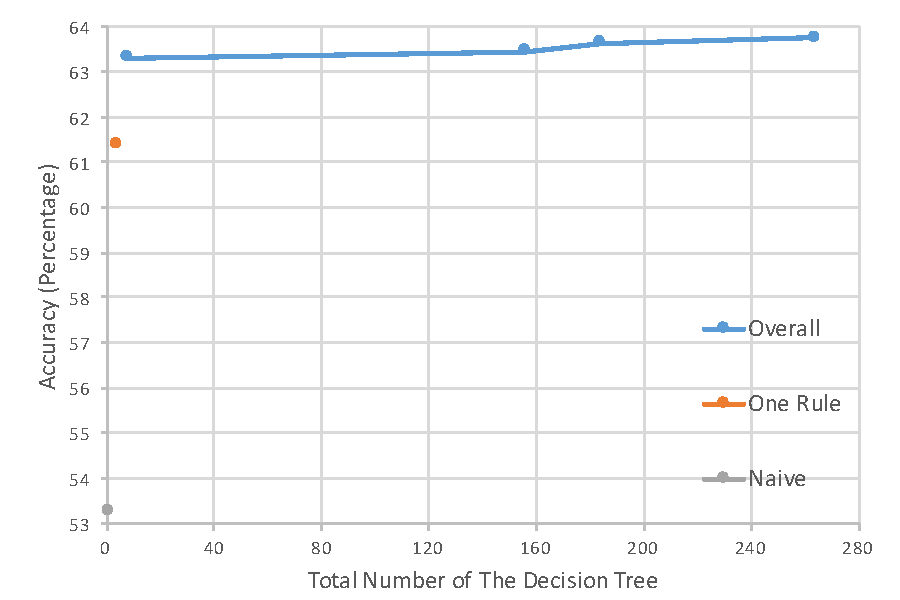
\includegraphics[width=0.6\textwidth]{figures/smart_default_optimal.pdf}
	\caption{Parsimony/accuracy comparison for Naive, One Rule, and Overall Prediction}
	\label{fig:smart_default_optimal}
\end{figure}

\begin{figure}
	\centering
	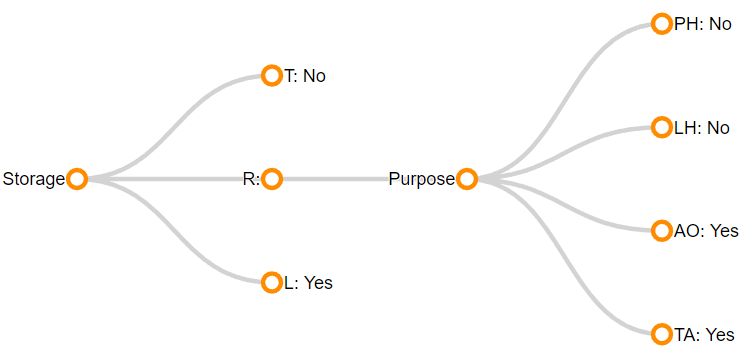
\includegraphics[width=0.6\textwidth]{figures/smartdefault001.png}
	\caption{A ``smart default'' setting with only 8 nodes (accuracy: 63.32\%). Parameter value abbreviations correspond to the ``code'' column in Table~\ref{tab:parameter2}.}
	\label{fig:smart_default_new}
\end{figure}


While the ``smart default'' setting makes a considerable improvement over a naive default, there is still a lot of room for improvement---even our best prediction model only correctly models on average 63.76\% of the user's desired settings. This should come at no surprise, as one of the most consistent findings in the field of privacy is that people differ substantially in their privacy preferences~\cite{knijnenburg2013dimensionality}. As a result, our ``one-size fits all'' default setting---smart as it may be---is not very accurate. Recent work in the field of privacy suggest to \emph{tailor} the privacy settings to the user to accommodate for these interpersonal differences~\cite{knijnenburg2017}. Our previous work therefore moved beyond ``smart default'' settings by clustering participants with similar privacy preferences and creating a set of ``smart profiles'' covering each of the clusters~\cite{bahiratiui2018}. The idea is that the accuracy of the tree for each cluster will likely exceed the accuracy of our overall prediction model. 

In the remainder of this section we apply existing and new clustering methods with the aim of creating separate ``smart profiles" for each cluster. As our goal is to develop simple, understandable profiles, we keep the parsimony/accuracy trade-off in mind during this process.


\subsection{Attitude-Based Clustering}
%As shown in Figure~\ref{fig:mediation_test}, 
Our statistical results indicate that the effects of scenario parameters on users' decisions are mediated by their attitudes (Risk, Comfort, Appropriateness, Expectedness and Usefulness). Therefore, our first attempt to develop ``smart profiles'' is to cluster participants with similar attitudes towards the 12 scenarios they evaluated. We averaged the values per attitude across each participant's 12 answers, and ran a \textit{k-means} clustering algorithm to divide them into 2, 3, 4, 5, and 6 clusters. We then added the participants' cluster assignments back to our original dataset, and ran the J48 decision tree algorithm on the dataset with this additional \emph{Cluster} attribute for each number of clusters, varying the Confidence Factor from 0.01 to 0.25 with increments of 0.01. The results are summarized in Figure~\ref{fig:attitudesum}, which displays the most accurate solution for any given tree size and number of clusters.

%Actual profile numbers, average tree sizes per profile, and accuracies for resulting solutions are reported in Table~\ref{tab:attitude_results}.

All of the resulting decision trees have \emph{Cluster} as the root node. This justifies our approach, because it indicates that the \emph{Cluster} parameter is a very effective for predicting users' decisions. It also allows us to split the decision trees at the root node, and a create different ``smart profile'' for each subtree/cluster. Note that for some solutions two clusters end up with the same decision tree, which effectively reduces the number of profiles by 1.

\begin{figure}
	\centering
	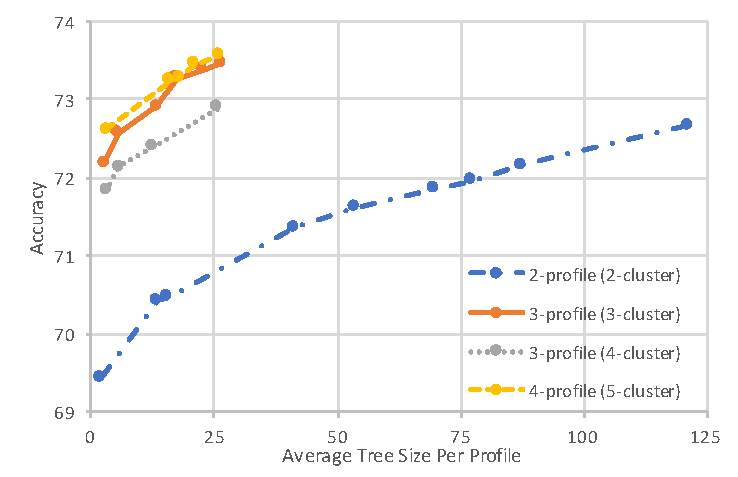
\includegraphics[width=0.95\textwidth]{figures/attitudeSum2.pdf}
	\caption{Parsimony/accuracy comparison for attitude-based clustering}
	\label{fig:attitudesum}
\end{figure}

%\begin{table}
%	\centering
%	\caption{Attitude Clustering Results}
%	\label{tab:attitude_results}
%	\begin{tabular}{c||c|c|c||c|c|c||c|c|c||c|c|c} \hline
%	&  \multicolumn{3}{c||}{2-cluster} & \multicolumn{3}{c||}{3-cluster} & \multicolumn{3}{c||}{4-cluster}  & \multicolumn{3}{c}{5-cluster} \\ \hline
%	Confi- &  & Avg & Accu- &  & Avg & Accu- &  & Avg & Accu- &  & Avg & Accu- \\
%	dence  &  & tree & racy &  & tree & racy &  & tree & racy &  & Tree & racy \\
%	  & * & size &  & * & size &  & * & size &  & * & size &  \\ 
%	Factor &  & /prof. &  &  & /prof. & &  & /prof. & &  & /prof. \\ \hline
%0.01 & 2 & 3 & 69.44\% & 3 & 3.67 & 72.19\% & 3 & 4 & 71.82\% & 4 & 4 & 72.61\% \\
%0.02 & 2 & 3 & 69.44\% & 3 & 6.33 & 72.57\% & 3 & 4 & 71.82\% & 4 & 4 & 72.61\% \\
%0.03 & 2 & 3 & 69.44\% & 3 & 6.33 & 72.57\% & 3 & 4 & 71.82\% & 4 & 4 & 72.61\% \\
%0.04 & 2 & 3 & 69.44\% & 3 & 6.33 & 72.57\% & 3 & 6.67 & 72.14\% & 4 & 4 & 72.61\% \\
%0.05 & 2 & 3 & 69.44\% & 3 & 6.33 & 72.57\% & 3 & 6.67 & 72.14\% & 4 & 4 & 72.61\% \\
%0.06 & 2 & 3 & 69.44\% & 3 & 6.33 & 72.57\% & 3 & 6.67 & 72.14\% & 4 & 4 & 72.61\% \\
%0.07 & 2 & 3 & 69.44\% & 3 & 6.33 & 72.57\% & 3 & 6.67 & 72.14\% & 4 & 4 & 72.61\% \\
%0.08 & 2 & 3 & 69.44\% & 3 & 6.33 & 72.57\% & 3 & 6.67 & 72.14\% & 4 & 4 & 72.61\% \\
%0.09 & 2 & 3 & 69.44\% & 3 & 6.33 & 72.57\% & 3 & 6.67 & 72.14\% & 4 & 4 & 72.61\% \\
%0.1 & 2 & 14.5 & 70.43\% & 3 & 6.33 & 72.57\% & 3 & 6.67 & 72.14\% & 4 & 4 & 72.61\% \\
%0.11 & 2 & 14.5 & 70.43\% & 3 & 6.33 & 72.57\% & 3 & 6.67 & 72.14\% & 4 & 4 & 72.61\% \\
%0.12 & 2 & 14.5 & 70.43\% & 3 & 6.33 & 72.57\% & 3 & 6.67 & 72.14\% & 4 & 4 & 72.61\% \\
%0.13 & 2 & 14.5 & 70.43\% & 3 & 6.33 & 72.57\% & 3 & 6.67 & 72.14\% & 4 & 4 & 72.61\% \\
%0.14 & 2 & 14.5 & 70.43\% & 3 & 6.33 & 72.57\% & 3 & 6.67 & 72.14\% & 4 & 4 & 72.61\% \\
%0.15 & 2 & 16.5 & 70.47\% & 3 & 6.33 & 72.57\% & 3 & 6.67 & 72.14\% & 4 & 4 & 72.61\% \\
%0.16 & 2 & 16.5 & 70.47\% & 3 & 14.33 & 72.91\% & 3 & 6.67 & 72.14\% & 4 & 4 & 72.61\% \\
%0.17 & 2 & 16.5 & 70.47\% & 3 & 18.33 & 73.26\% & 3 & 6.67 & 72.14\% & 4 & 4 & 72.61\% \\
%0.18 & 2 & 42.5 & 71.37\% & 3 & 18.33 & 73.26\% & 3 & 6.67 & 72.14\% & 4 & 4 & 72.61\% \\
%0.19 & 2 & 54.5 & 71.62\% & 3 & 18.33 & 73.26\% & 3 & 6.67 & 72.14\% & 4 & 4 & 72.61\% \\
%0.2 & 2 & 54.5 & 71.62\% & 3 & 18.33 & 73.26\% & 3 & 6.67 & 72.14\% & 4 & 17 & 73.24\% \\
%0.21 & 2 & 70.5 & 71.85\% & 3 & 23.67 & 73.37\% & 3 & 13.33 & 72.39\% & 4 & 17 & 73.24\% \\
%0.22 & 2 & 78.5 & 71.96\% & 3 & 27.67 & 73.47\% & 3 & 13.33 & 72.39\% & 4 & 19 & 73.29\% \\
%0.23 & 2 & 88.5 & 72.16\% & 3 & 27.67 & 73.47\% & 3 & 13.33 & 72.39\% & 4 & 22 & 73.46\% \\
%0.24 & 2 & 88.5 & 72.16\% & 3 & 27.67 & 73.47\% & 3 & 13.33 & 72.39\% & 4 & 22 & 73.46\% \\
%0.25 & 2 & 122.5 & 72.66\% & 3 & 27.67 & 73.47\% & 3 & 26.67 & 72.90\% & 4 & 27 & 73.56\% \\ \hline
%	\end{tabular}
%\bigskip
%\footnotesize
%
%\textbf{$*$}: Actual Profile Number.
%\end{table}

%As shown in Table~\ref{tab:attitude_results}, as the Confidence Factor increases from 0.01 to 0.25, the actual resulting profile number of 2-cluster solution keeps at 2, 
For the 2-cluster solutions (the blue line in Figure~\ref{fig:attitudesum}), the highest accuracy is 72.66\%, which is a 14.0\% improvement over the best single ``smart default'' setting. However, this tree has an average of 121.5 nodes per profile. In comparison, the most parsimonious solution has only 1 node (``disable all'') for one of the clusters, and 3 nodes (``disable sharing with third parties'') for the other cluster (see Figure~\ref{fig:att_2_profile}). This solution still has an accuracy of 69.44\%, which is still an 8.9\% increase over the best single ``smart default'' setting.

\begin{figure}
	\centering
	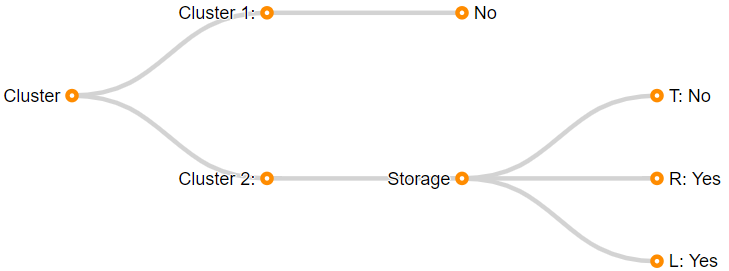
\includegraphics[width=0.8\textwidth]{figures/fit_2_profile001.png}
	\caption{The most parsimonious 2-profile attitude-based solution (2 nodes/profile, accuracy: 69.44\%). Parameter value abbreviations correspond to the ``code'' column in Table~\ref{tab:parameter2}.}
	\label{fig:att_2_profile}
\end{figure}

For the 3-cluster solutions (the orange line in Figure~\ref{fig:attitudesum}), the highest accuracy of 73.47\% is achieved by a set of trees with 26.67 nodes on average (a minimal improvement of 1.1\% over the best 2-cluster solution, but with simpler trees), while the most parsimonious solution has a ``disable all'' and an ``enable all'' tree, plus a tree that is the same as the most parsimonious smart default setting (see Figure~\ref{fig:smart_default_new}). This solution has an accuracy of 72.19\%, which is a 4.0\% increase over the most parsimonious 2-cluster solution.

The 4-cluster solutions (the grey line in Figure~\ref{fig:attitudesum}) all result in ``over-clustering'': all solutions based on the 4-cluster \emph{Cluster} parameter result in two profiles with the same subtree, effectively resulting in a 3-profile solution. The accuracy of these solutions is actually lower than the accuracy of similar 3-cluster solutions, so we will not discuss them here.

The 5-cluster solutions (the yellow line in Figure~\ref{fig:attitudesum}) are also ``over-clustered'', resulting in 4 profiles. The highest accuracy of 73.56\% is achieved by a set of trees with 26 nodes---this is about the same accuracy and parsimony as the most accurate 3-cluster solution. The same holds for the most parsimonious 5-cluster solution, which has a similar accuracy and parsimony as the most parsimonious 3-cluster solution.

The accuracy of the 6-cluster solutions (which result in either 4- or 5-profile solutions) is lower than the accuracy of similar 5-cluster solutions. Therefore, we will not further discuss these results.

Reflecting upon the attitude-based clustering results, we observe in Figure~\ref{fig:attitudesum} that there is indeed a trade-off between accuracy and parsimony: the most parsimonious results are less accurate, but the most accurate results are more complex. Moreover, the 2-profile solutions are about 5\% less accurate than the 3-profile solutions at any level of complexity. The 4-profile solutions do not improve the solution much further, though.

The 3-profile solution with an average of 18.33 nodes per profile and 73.26\% accuracy provides a nice compromise between accuracy and parsimony. Part of this decision tree is shown in Figure~\ref{fig:attitude_3profile}: it contains one ``disable all'' profile, one ``enable all'' profile, and a more complex profile with 55 nodes that disallows sharing with third parties and allows remote and local storage depending on the purpose (not further shown).

\begin{figure}
	\centering
	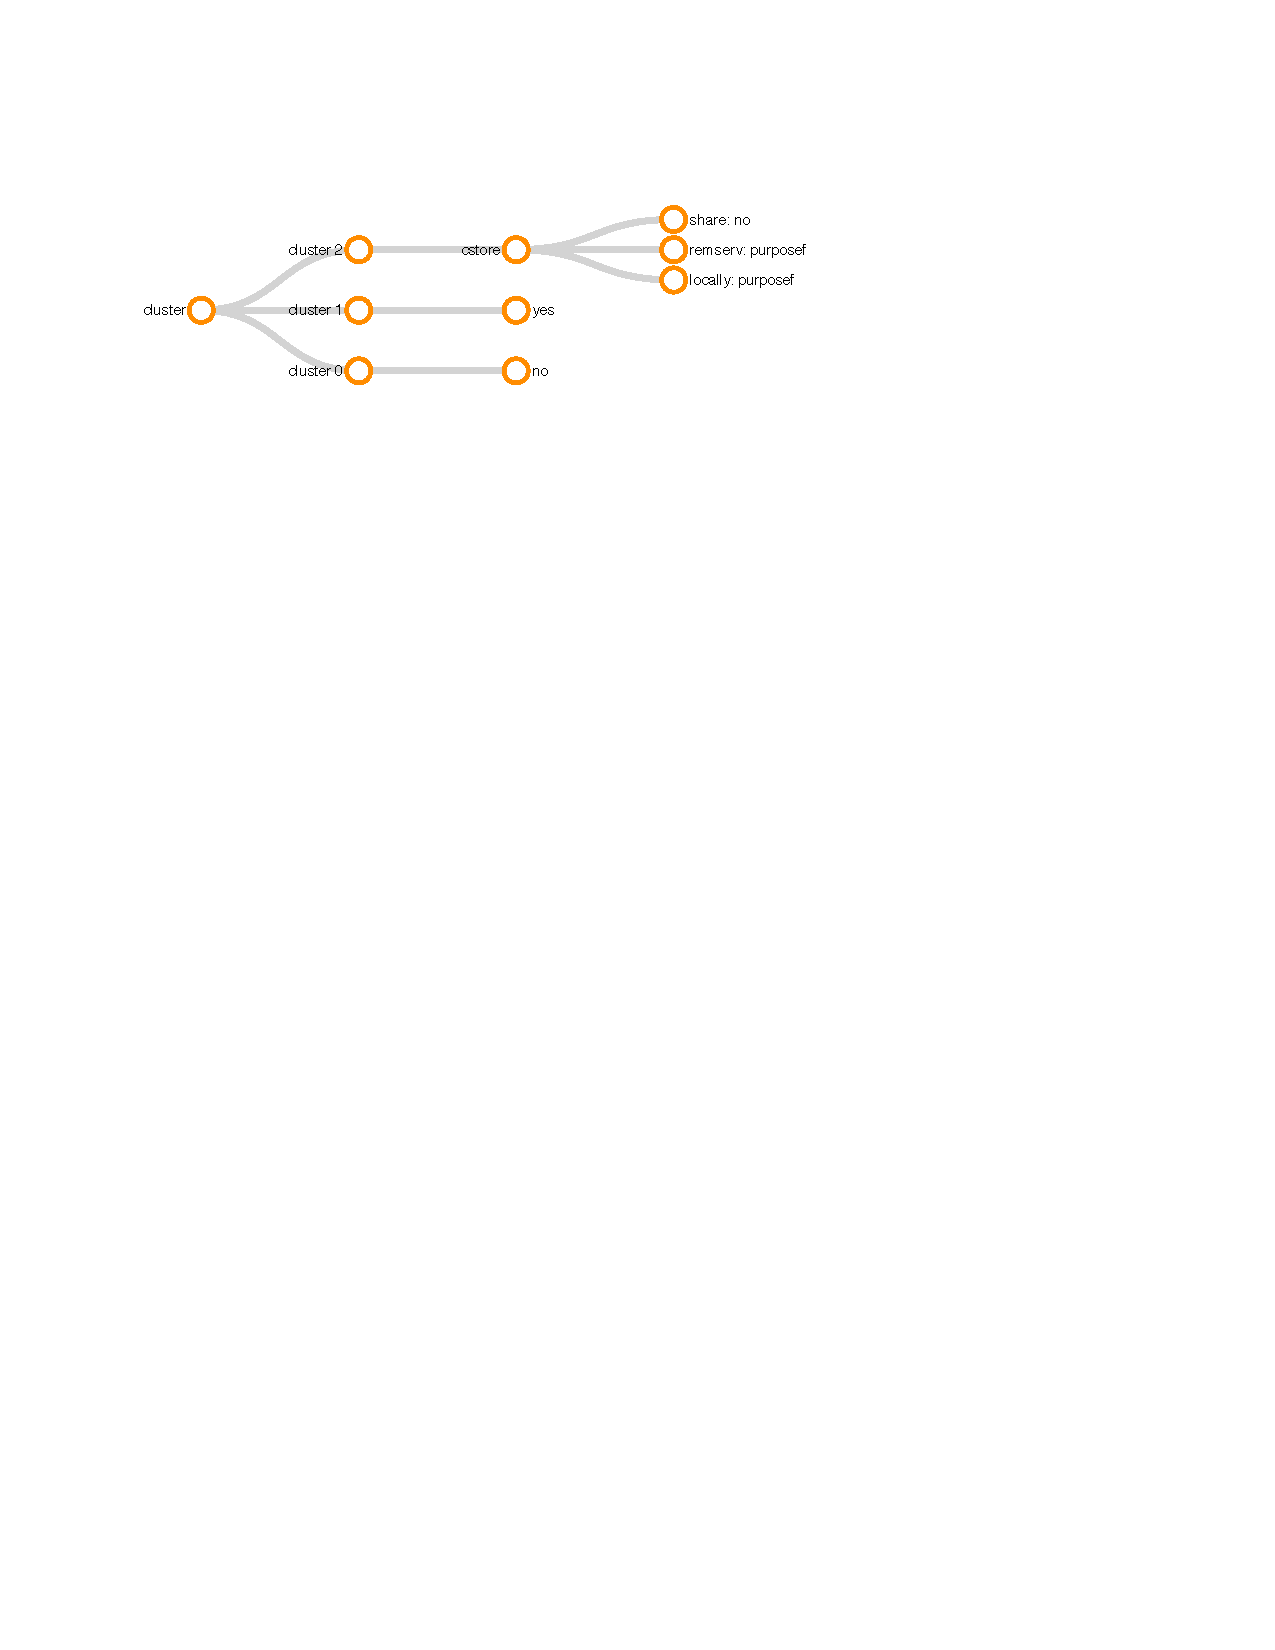
\includegraphics[width=0.7\textwidth]{figures/attitude_3_profile.pdf}
	\caption{A 3-profile solution example of attitude-based clustering (18.33 nodes/profile, accuracy: 73.26\%). Parameter value abbreviations correspond to the ``code'' column in Table~\ref{tab:parameter2}.}
	\label{fig:attitude_3profile}
\end{figure}

\subsection{Agglomerative Clustering}
The attitude-based clustering approach requires knowledge of users' attitudes towards the household IoT information-sharing scenarios, which may not always be available. We developed an alternative method for finding ``smart profiles'' that follows a hierarchical bottom-up (or agglomerative) approach, using users' decisions only. This method first fits a separate decision tree for each participant, and then iteratively merges these trees based on similarity. In our previous work~\cite{bahiratiui2018} only 10 out of the 200 users in the dataset had unique trees fitted to them (all others had an ``enable all'' or ``disable all'' tree), making the merging of trees a rather trivial affair. Our current dataset has many more participants, and is more complex, making the agglomerative clustering approach more challenging but also more meaningful. 

In the first step, 283 participants' decision trees predict ``enable all'', 414 participants' decision trees predict ``disable all'', while the remaining 436 participants have a multi-node decision tree.

In the second step, a new decision tree is generated for each possible pair of participants in the ``multi-node group''. The accuracy of the new tree is compared against the weighted average of the accuracies of the original trees. The pair with smallest reduction in accuracy is merged, leaving 435 clusters for the next round of merging. If two or more candidate pairs have the same smallest reduction in accuracy, priority is given to the pair with the most parsimonious resulting tree (i.e., with smallest number of nodes). If there are still multiple pairs that tie on this criterion, the first pair is picked. The second step is repeated until it reaches the predefined number of clusters, and the entire procedure is repeated with 20 random starts to avoid local optima.

%\begin{table}
%	\centering
%	\caption{Agglomerative Clustering Results for \textit{Multi-node Group}}
%	\label{tab:conglo_results}
%	\begin{tabular}{c||c|c||c|c||c|c} \hline
%	Confi- &  \multicolumn{2}{c||}{4-cluster} & \multicolumn{2}{c||}{5-cluster} & \multicolumn{2}{c}{6-cluster}  \\ \cline{2-7}
%	dence & Average & Accuracy & Average & Accuracy & Average & Accuracy\\
%	Factor & Nodes/Profile & & Nodes/Profile &  & Nodes/Profile &\\ \hline
%	0.01 & 2.5 & 79.40\% & 3 & 80.35\% & 3.83 & 80.68\% \\
%	0.02 & 2.5 & 79.29\% & 3 & 80.26\% & 3.33 & 80.60\% \\
%	0.03 & 2.5 & 79.23\% & 3 & 80.29\% & 3.83 & 80.66\% \\
%	0.04 & 2.5 & 79.23\% & 3 & 80.23\% & 3.83 & 80.60\% \\
%	0.05 & 2.5 & 79.31\% & 3 & 80.23\% & 3.83 & 80.48\% \\
%	0.06 & 2.5 & 79.29\% & 3 & 80.11\% & 3.83 & 80.59\% \\
%	0.07 & 2.5 & 79.39\% & 3 & 80.13\% & 3.83 & 80.56\% \\
%	0.08 & 2.5 & 79.29\% & 3 & 80.13\% & 4.50 & 80.56\% \\
%	0.09 & 2.5 & 79.31\% & 3 & 80.05\% & 3.83 & 80.43\% \\
%	0.10 & 2.5 & 79.27\% & 3 & 79.86\% & 3.83 & 80.32\% \\
%	0.11 & 2.5 & 79.21\% & 3.6 & 79.81\% & 4.50 & 80.59\% \\
%	0.12 & 2.5 & 79.21\% & 3 & 79.94\% & 4.50 & 80.59\% \\
%	0.13 & 2.5 & 79.14\% & 3 & 79.71\% & 4.33 & 79.96\% \\
%	0.14 & 2.5 & 79.18\% & 3.6 & 79.80\% & 4.50 & 80.26\% \\
%	0.15 & 2.5 & 78.99\% & 3 & 79.85\% & 5.67 & 79.96\% \\
%	0.16 & 2.5 & 79.08\% & 3.6 & 79.61\% & 6.83 & 80.59\% \\
%	0.17 & 2.5 & 78.99\% & 3.6 & 79.70\% & 9.83 & 79.81\% \\
%	0.18 & 2.5 & 78.94\% & 3.6 & 79.73\% & 5.83 & 80.15\% \\
%	0.19 & 7.5 & 78.62\% & 7.6 & 79.31\% & 9.83 & 79.71\% \\
%	0.2 & 6.5 & 78.56\% & 13 & 79.19\% & 11.67 & 79.23\% \\
%	0.21 & 4.5 & 78.56\% & 11 & 79.01\% & 9.67 & 79.68\% \\
%	0.22 & 6.5 & 78.49\% & 8.4 & 79.06\% & 8.33 & 79.68\% \\
%	0.23 & 6.5 & 78.81\% & 11.8 & 79.17\% & 15.67 & 79.66\% \\
%	0.24 & 6.5 & 78.87\% & 13.2 & 78.97\% & 13.00 & 79.51\% \\
%	0.25 & 11.5 & 78.41\% & 17.2 & 78.80\% & 11.67 & 79.41\% \\ \hline
%	\end{tabular}
%\end{table}


To fit the trees, we use the J48 classifier with a Confidence Factor ranging from 0.01 to 0.25 with increments of 0.01. Surprisingly, smaller tree sizes result in a \emph{higher} accuracy for agglomerative clustering (see Figure~\ref{fig:conglosum}). This suggests that without extensive trimming, our agglomerative approach arguably overfits the data, resulting in a lower level of cross-validated accuracy.

\begin{figure}
	\centering
	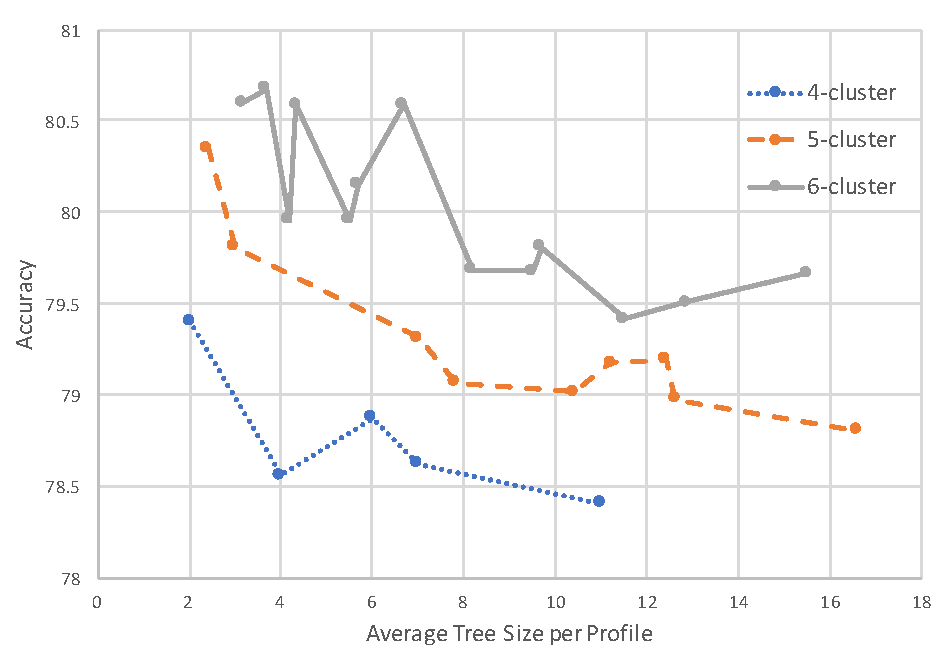
\includegraphics[width=0.7\textwidth]{figures/congloSum2.pdf}
	\caption{Parsimony/accuracy comparison for agglomerative clustering}
	\label{fig:conglosum}
\end{figure}

The best 4-cluster solution has an average of 2 nodes per profile and an accuracy of 79.40\%---a 24.53\% improvement over the ``smart default'', and a 7.9\% increase over the most accurate 5-cluster/4-profile attitude-based clustering solution. The decision trees are shown in Figure~\ref{fig:conglo_4_profile001}: aside from the ``enable all'' and ``disable all'' profiles, there  is a ``disable sharing with third parties'' profile and a ``local storage only'' profile.

\begin{figure}
	\centering
	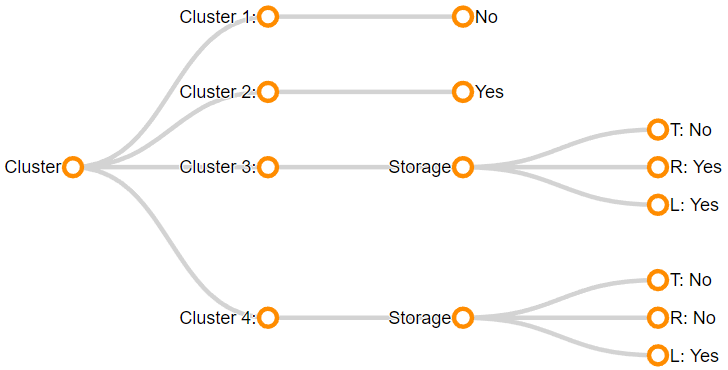
\includegraphics[width=0.6\textwidth]{figures/conglo_4_profile001.png}
	\caption{The best 4-profile agglomerative clustering solution (2 nodes/profile, accuracy: 79.40\%). Parameter value abbreviations correspond to the ``code'' column in Table~\ref{tab:parameter2}.}
	\label{fig:conglo_4_profile001}
\end{figure}

The best 5-cluster solution has an average of 2.4 nodes per profile and an accuracy of 80.35\%---a 26.02\% improvement over the ``smart default'', but only a 1.2\% improvement over the 4-cluster agglomerative solution. The decision trees are shown in Figure~\ref{fig:conglo_5_profile001}: it has the same profiles as the 4-cluster solution, plus an ``allow automation and alerts, but don't track my presence or location in the house'' profile.

\begin{figure}
	\centering
	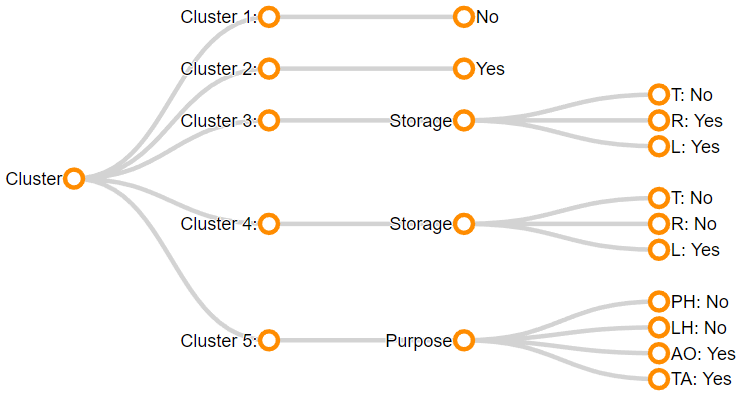
\includegraphics[width=0.6\textwidth]{figures/conglo_5_profile001.png}
	\caption{The best 5-profile agglomerative clustering solution (2.4 nodes/profile, Accuracy: 80.35\%). Parameter value abbreviations correspond to the ``code'' column in Table~\ref{tab:parameter2}.}
	\label{fig:conglo_5_profile001}
\end{figure}

Finally, the best 6-cluster solution\footnote{There is another solution with slightly fewer nodes per profile (2.67) and a slightly lower accuracy (80.60\%).} has an average of 3.17 nodes per profile and an accuracy of 80.68\%---a 26.54\% improvement over the ``smart default'', but no substantial improvement over the 5-cluster agglomerative solution. The decision trees are shown in Figure~\ref{fig:conglo_6_profile001}: it has the same profiles as the 5-cluster solution, plus a profile that allows local storage for anything, plus remote storage for any reason except for user profiling (i.e., to recommend other services or to give the user insight in their behavior).

\begin{figure}
	\centering
	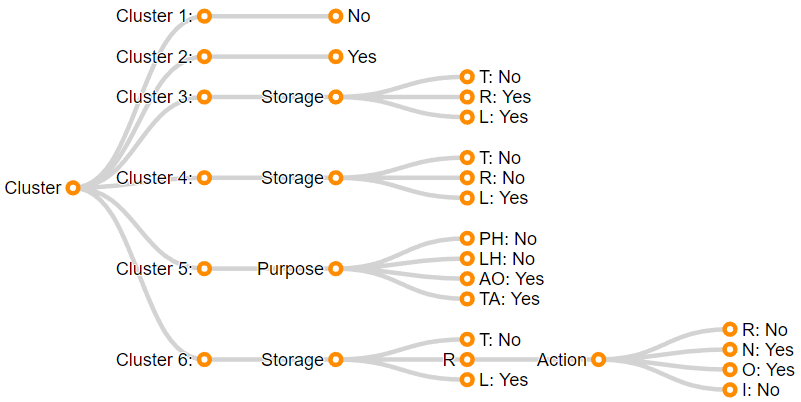
\includegraphics[width=0.6\textwidth]{figures/conglo_6_profile001.png}
	\caption{The best 6-profile agglomerative clustering solution (3.17 nodes/profile, Accuracy: 80.68\% ). Parameter value abbreviations correspond to the ``code'' column in Table~\ref{tab:parameter2}.}
	\label{fig:conglo_6_profile001}
\end{figure}

\subsection{Fit-Based Clustering}
We now present a ``fit-based'' clustering approach that, like the agglomerative approach, clusters participants without using any additional information. Instead, it uses the fit of the tree models to bootstrap the process of sorting participants into different clusters. The steps of our algorithm are as follows:
\begin{itemize}
	\item \textbf{Random starts:} We randomly divide participants into $k$ separate groups, and learn a tree for each group. This is repeated until a non-trivial starting solution (i.e., with distinctly different trees per group) is found. 
	
	\item \textbf{Iterative improvements:} Once each of the $k$ groups has a unique decision tree, we test for each participant which of the $k$ trees best represents their 12 decisions. If this is the tree of a different group, we switch the participant to this group. Once all participants are evaluated and put in the group of their best-fitting tree, the tree in each group is re-learned with the data of the new group members. This then prompts another round of evaluations, and this process continues until no further switches are performed.
	
	\item \textbf{Repeat}: Since this process is influenced by random chance, it is repeated 1,000 times in its entirety to find the optimal solution. Cross-validation is performed in the final step to prevent over-fitting.
\end{itemize}

We perform this approach to obtain 2-, 3-, 4-, and 5-cluster solutions. To fit the trees, we use the J48 classifier with a Confidence Factor ranging from 0.01 to 0.25 with increments of 0.01. The best results are summarized in Figure~\ref{fig:fitsum}.

\begin{figure}
	\centering
	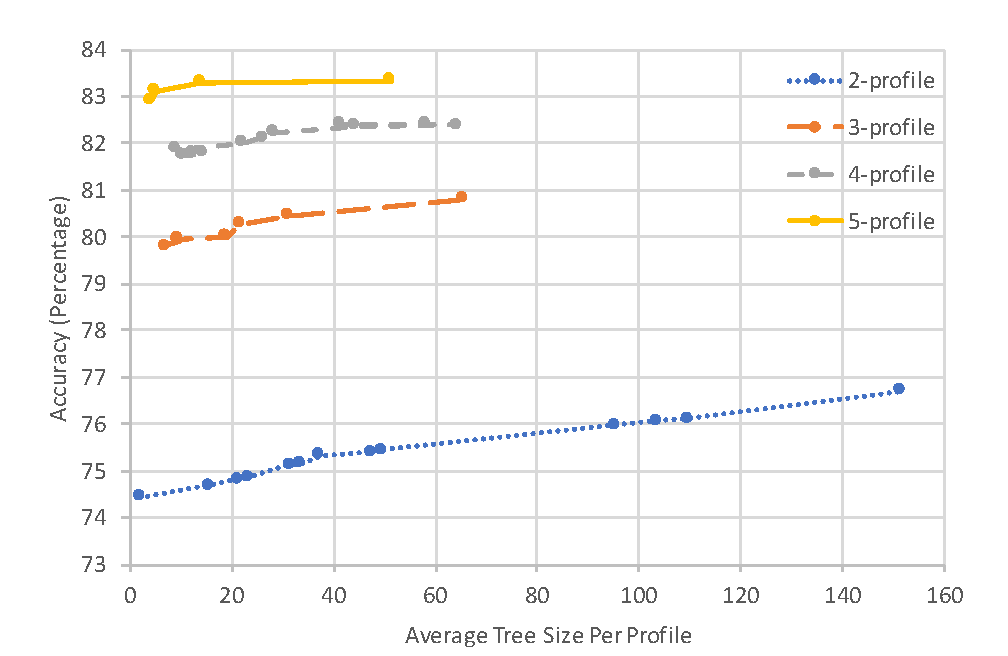
\includegraphics[width=0.7\textwidth]{figures/fitSum.pdf}
	\caption{Parsimony/accuracy comparison for fit-based clustering}
	\label{fig:fitsum}
\end{figure}

For the 2-cluster solutions (the blue line in Figure~\ref{fig:fitsum}), the highest accuracy is 76.72\%---a 20.33\% improvement over the ``smart default'' setting and a 5.6\% improvement over the most accurate 2-cluster attitude-based solution. However, this tree has an average of 151.5 nodes per profile. The most parsimonious solution is exactly the same as the most parsimonious 2-cluster attitude-based solution (see Figure~\ref{fig:att_2_profile}), but with a higher accuracy (74.43\%).

For the 3-cluster solutions (the orange line in Figure~\ref{fig:fitsum}), the highest accuracy of 80.81\% is achieved by a set of trees with 65.33 nodes on average. This is a 26.74\% improvement over the ``smart default'', a 10.0\% improvement over the most accurate 3-cluster attitude-based solution (but at a cost of lower parsimony), and a 5.2\% improvement over the best 2-cluster fit-based solution. The most parsimonious solution, on the other hand, has 7 nodes on average, with an accuracy of 79.80\%, thereby still outperforming all other 3-profile solutions. The decision trees for this solution are shown in Figure~\ref{fig:fit_3_profile001}.

\begin{figure}
	\centering
	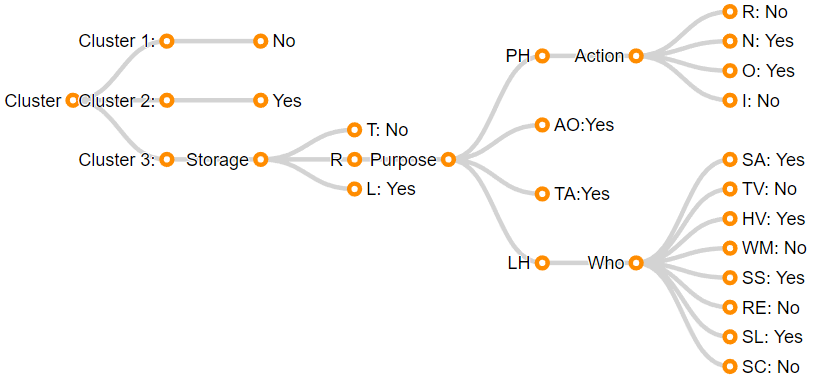
\includegraphics[width=0.6\textwidth]{figures/fit_3_profile001.png}
	\caption{The most parsimonious 3-profile fit-based solution (7 nodes/profile, accuracy: 79.80\%). Parameter value abbreviations correspond to the ``code'' column in Table~\ref{tab:parameter2}.}
	\label{fig:fit_3_profile001}
\end{figure}

For the 4-cluster solutions (the grey line in Figure~\ref{fig:fitsum}), the highest accuracy of 82.41\% is achieved by a set of trees with 58.25 nodes on average. This is a 29.25\% improvement over the ``smart default'', a 3.8\% improvement over the 4-cluster agglomerative solution (but at a cost of lower parsimony), and a 2.0\% improvement over the best 3-cluster fit-based solution. The most parsimonious solution, on the other hand, has 9.25 nodes on average, with an accuracy of 81.88\%. It still outperforms all other 4-profile solutions, but the agglomerative solution is more parsimonious. The decision trees for this solution are shown in Figure~\ref{fig:fit_4_profile010}.

\begin{figure}
	\centering
	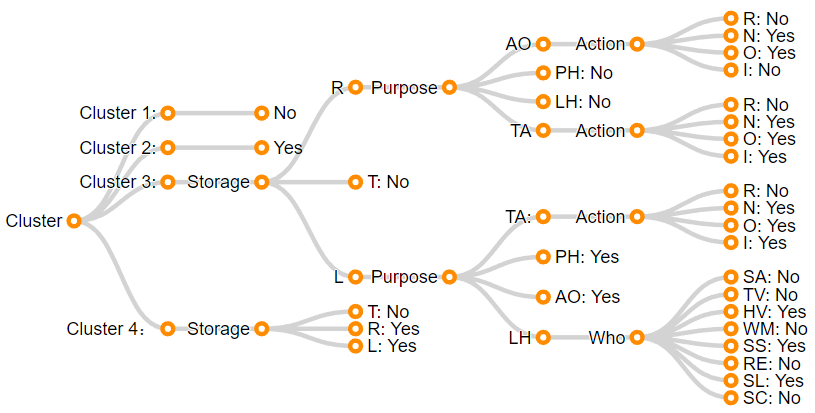
\includegraphics[width=0.6\textwidth]{figures/fit_4_profile010.png}
	\caption{The most parsimonious 4-profile fit-based solution (9.25 nodes/profile, accuracy: 81.88\% ). Parameter value abbreviations correspond to the ``code'' column in Table~\ref{tab:parameter2}.}
	\label{fig:fit_4_profile010}
	\vspace{20px}
\end{figure}

For the 5-cluster solutions (the yellow line in Figure~\ref{fig:fitsum}), the highest accuracy of 83.35\% is achieved by a set of trees with 51.4 nodes on average. This is a 30.05\% improvement over the ``smart default'', a 3.8\% improvement over the 5-cluster agglomerative solution (but at a cost of lower parsimony), and a 1.1\% improvement over the best 4-cluster fit-based solution. The most parsimonious solution, on the other hand, has 4.2 nodes on average, with an accuracy of 82.92\%. It still outperforms the 5-profile agglomerative solution, but it is slightly less parsimonious. The decision trees for this solution are shown in Figure~\ref{fig:fit_5_profile001}.

\begin{figure}
	\centering
	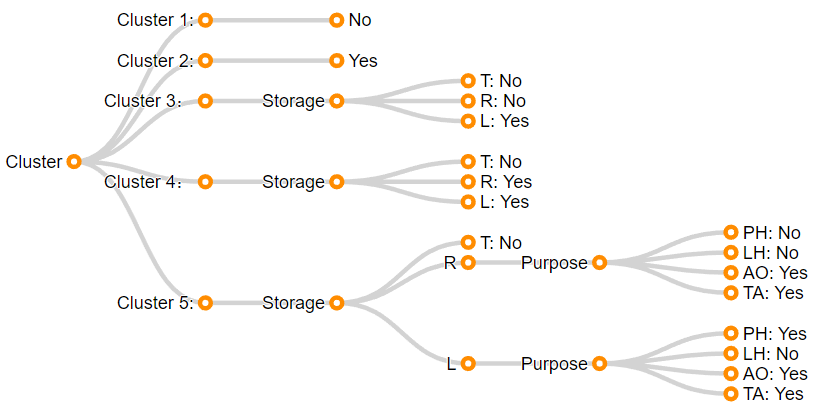
\includegraphics[width=0.6\textwidth]{figures/fit_5_profile001.png}
	\caption{The most parsimonious 5-profile fit-based solution (4.2 nodes/profile, accuracy: 82.92\% ). Parameter value abbreviations correspond to the ``code'' column in Table~\ref{tab:parameter2}.}
	\label{fig:fit_5_profile001}
\end{figure}

%\begin{table}
%	\centering
%	\caption{Fit-Based Clustering Results}
%	\label{tab:fit_results}
%	\begin{tabular}{c||c|c||c|c||c|c||c|c} \hline
%		 &  \multicolumn{2}{c||}{2-profile} & \multicolumn{2}{c||}{3-profile} & \multicolumn{2}{c||}{4-profile}  & \multicolumn{2}{c}{5-profile} \\ \hline
%		Confi- & Average & Accu- & Average & Accu- & Average & Accu- & Average & Accu- \\
%		dence  & TreeSize & racy & TreeSize & racy & TreeSize &  & TreeSize & racy \\ 
%		Factor & /profile &  & /profile & & /profile & & /profile \\ \hline
%		0.01 & 2.5 & 74.43\%	& 7.33	& 79.80\%	& 10.5	& 81.73\%	& 4.4	& 82.92\%  \\ %\cline{2-5}
%		0.02 & 2.5 & 74.43\%	& 10	& 79.91\%	& 10.5	& 81.73\%	& 4.4	& 82.92\%  \\ %\cline{2-5}
%		0.03 & 2.5 & 74.43\%	& 10	& 79.91\%	& 10.5	& 81.73\%	& 5.2	& 83.11\%  \\ %\cline{2-5}
%		0.04 & 2.5 & 74.43\%	& 10	& 79.91\%	& 14.5	& 81.78\%	& 5.2	& 83.11\%  \\ %\cline{2-5}
%		0.05 & 2.5 & 74.43\%	& 10	& 79.91\%	& 12.5	& 81.8\%	& 5.2	& 83.11\%  \\ %\cline{2-5}
%		0.06 & 2.5 & 74.43\%	& 10	& 79.91\%	& 12.5	& 81.8\%	& 5.2	& 83.11\%  \\ %\cline{2-5}
%		0.07 & 2.5 & 74.43\%	& 10	& 79.91\%	& 12.5	& 81.8\%	& 14	& 83.30\%  \\ %\cline{2-5}
%		0.08 & 2.5 & 74.43\%	& 10	& 79.91\%	& 12.5	& 81.8\%	& 14	& 83.30\%  \\ %\cline{2-5}
%		0.09 & 16  & 74.69\%	& 10	& 79.95\%	& 12.5	& 81.8\%	& 14	& 83.30\%  \\ %\cline{2-5}
%		0.10 & 16  & 74.69\%	& 10	& 79.95\%	& 9.5	& 81.88\%	& 14	& 83.30\%  \\ %\cline{2-5}
%		0.11 & 22  & 74.82\%	& 10	& 79.95\%	& 22.5	& 82.00\%	& 14	& 83.30\%  \\ %\cline{2-5}
%		0.12 & 24  & 74.87\%	& 19.33	& 80.00\%	& 22.5	& 82.00\%	& 14	& 83.30\%  \\ %\cline{2-5}
%		0.13 & 32  & 75.13\%	& 22	& 80.27\%	& 22.5	& 82.00\%	& 14	& 83.30\%  \\ %\cline{2-5}
%		0.14 & 32  & 75.13\%	& 22	& 80.27\%	& 26.5	& 82.12\%	& 14	& 83.30\%  \\ %\cline{2-5}
%		0.15 & 34  & 75.16\%	& 22	& 80.27\%	& 28.5	& 82.23\%	& 14	& 83.30\%  \\ %\cline{2-5}
%		0.16 & 38  & 75.33\%	& 22	& 80.27\%	& 28.5	& 82.23\%	& 14	& 83.30\%  \\ %\cline{2-5}
%		0.17 & 48  & 75.39\%	& 22	& 80.27\%	& 28.5	& 82.23\%	& 14	& 83.30\%  \\ %\cline{2-5}
%		0.18 & 50  & 75.44\%	& 22	& 80.27\%	& 28.5	& 82.23\%	& 14	& 83.30\%  \\ %\cline{2-5}
%		0.19 & 50  & 75.44\%	& 22	& 80.27\%	& 44.5	& 82.36\%	& 14	& 83.30\%  \\ %\cline{2-5}
%		0.20 & 96  & 75.97\%	& 31.33	& 80.44\%	& 44.5	& 82.36\%	& 51.6	& 83.35\%  \\ %\cline{2-5}
%		0.21 & 104 & 76.07\%	& 31.33	& 80.44\%	& 44.5	& 82.36\%	& 51.6	& 83.35\%  \\ %\cline{2-5}
%		0.22 & 110 & 76.10\%	& 31.33	& 80.44\%	& 44.5	& 82.36\%	& 51.6	& 83.35\%  \\ %\cline{2-5}
%		0.23 & 110 & 76.10\%	& 65.67	& 80.81\%	& 64.5	& 82.39\%	& 51.6	& 83.35\%  \\ %\cline{2-5}
%		0.24 & 110 & 76.10\%	& 65.67	& 80.81\%	& 41.5	& 82.4\%	& 51.6	& 83.35\%  \\ %\cline{2-5}
%		0.25 & 152 & 76.72\%	& 65.67	& 80.81\%	& 58.5	& 82.41\%	& 51.6	& 83.35\%  \\ \hline
%	\end{tabular}
%\end{table}


\subsection{Discussion of machine learning results}
Figure~\ref{fig:summary} shows a comparison of the presented approaches. The X-axis represents the parsimony (higher average tree size per profile = lower parsimony); the Y-axis represents the accuracy. While the ``smart default'' setting makes a significant 15.3\% improvement over the naive default setting (``disable all''), we observe that having multiple ``smart profiles'' substantially increases the prediction accuracy even further. The fit-Based clustering algorithm performs the best out of all the approaches, followed by agglomerative clustering and attitude-based clustering. 

\begin{figure*}
	\centering
	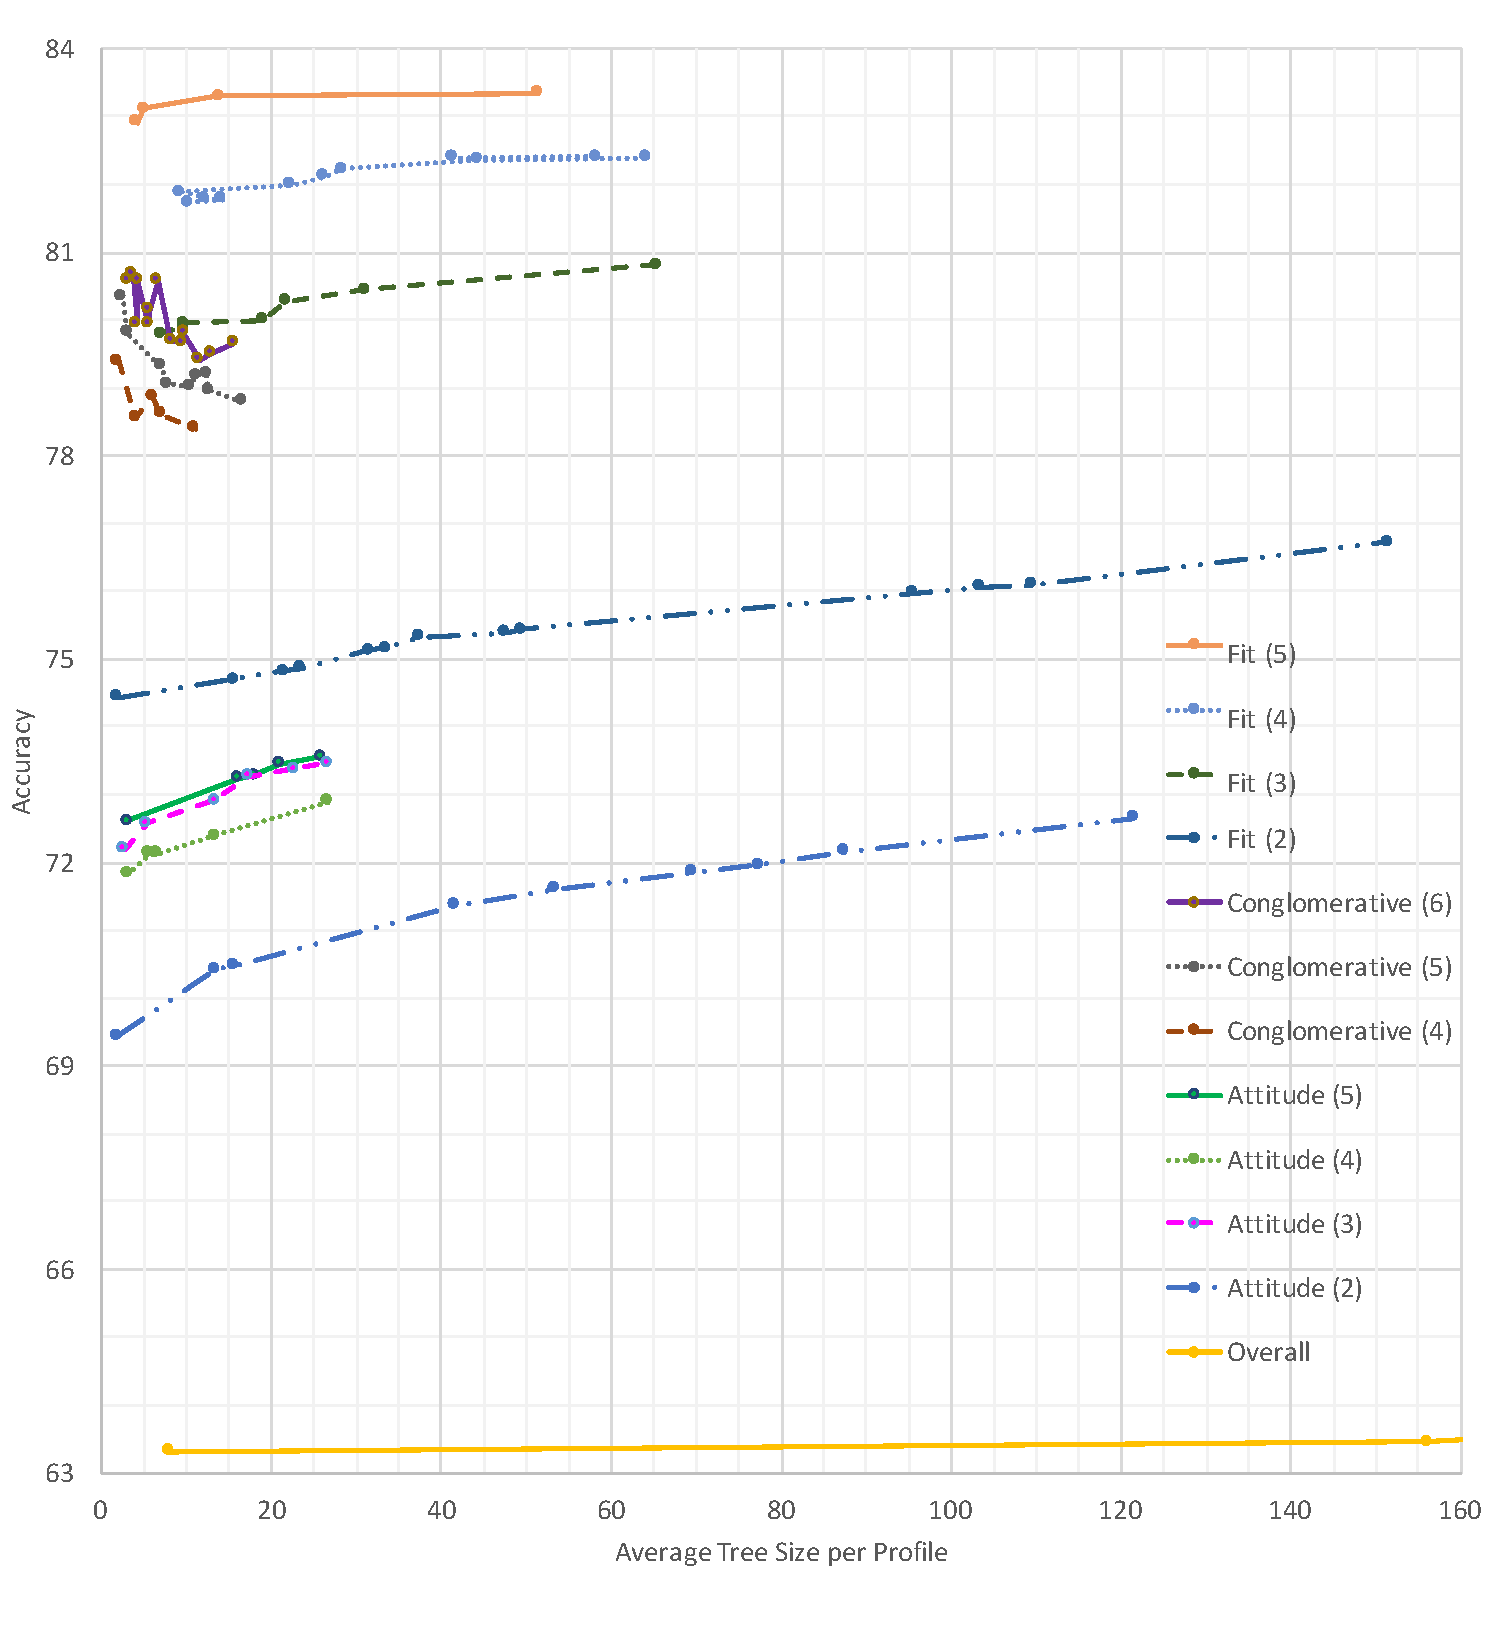
\includegraphics[width=0.7\textwidth]{figures/summaryAll.pdf}
	\caption{Summary of All our Approaches}
	\label{fig:summary}
\end{figure*}

The most parsimonious 2-profile fit-based solution (with an accuracy of 74.43\%) is the \emph{simplest} of all ``smart profile'' solutions: one profile is simply ``disable all'', while the other profile is the same as our OneR solution: ``disable sharing with third parties''. In fact, these profiles are so simple, that one might not even want to bother with presenting them to the user: in our current interface (see Figure~\ref{fig:interface2}) these defaults are incredibly easy for users to implement by themselves.

The same is true for the 4-profile agglomerative clustering solution (see Figure~\ref{fig:conglo_4_profile001}) and the 5-profile agglomerative clustering solution (see Figure~\ref{fig:conglo_5_profile001}): these profiles involve little more than a single high-level setting, which users can likely easily make by themselves. 

The 5-profile fit-based solution is the \emph{most accurate} of all ``smart profile'' solutions. The most parsimonious 5-profile fit-based clustering solution (Figure~\ref{fig:fit_5_profile001}) has an accuracy of 82.92\%. It has the following five profiles:
\begin{itemize}
	\item Enable all
	\item Enable local and remote storage, but disable third-party sharing
	\item Enable local storage only
	\item Enable local storage for everything except location-tracking, enable remote storage for everything except location- and presence-tracking, and disable third-party sharing
	\item Disable all
\end{itemize}
The fourth profile in this list specifies an interaction between between \textbf{Storage} and \textbf{Purpose}---something that is not possible in our current manual settings interface (which only allows interactions between \textbf{Who}, \textbf{What}, and \textbf{Purpose}). The next section will present a slightly altered interface that accommodates these profiles.

There is another 5-profile fit-based solution with a slightly higher accuracy (83.11\%) and a reasonably simple tree (5 nodes/profile on average). This solution is shown in Figure~\ref{fig:fit_5_profile003}. In this solution, the third profile (``enable local storage only'') is replaced by a slightly more complex profile (``enable local storage only, but not to recommend other services''). This profile specifies an additional interaction between \textbf{Storage} and \textbf{Action}. The next section will present a settings interface that accommodates this profile as well.

\begin{figure}
	\centering
	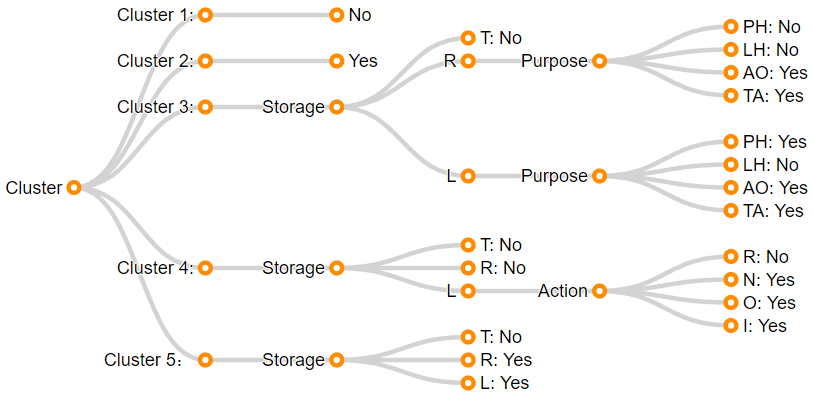
\includegraphics[width=0.6\textwidth]{figures/fit_5_profile003.png}
	\caption{A good 5-profile fit-based clustering solution (5 nodes/profile, Accuracy: 83.11\%). Parameter value abbreviations correspond to the ``code'' column in Table~\ref{tab:parameter2}.}
	\label{fig:fit_5_profile003}
\end{figure}

Other usable solutions are the 3-profile fit-based solution (Figure~\ref{fig:fit_3_profile001}) or the 4-profile fit-based solution (Figure~\ref{fig:fit_4_profile010}. However, like almost all of the less parsimonious solutions, these profiles involve higher-order interaction effects, e.g. between \textbf{Storage}, \textbf{Purpose}, and \textbf{Action}; and between \textbf{Storage}, \textbf{Purpose}, and \textbf{Who}. Consequently, a rather more complex interface is needed to accommodate these default profiles.

\section{Privacy-Setting Prototype Design Using Machine Learning Results (original work)}\label{sec:design_ml}
In Section~\ref{sec:design_stat} we developed a prototype interface that household IoT users can use to manually set their privacy settings (see Figure~\ref{fig:interface2}). Our machine learning analysis (Section~\ref{sec:predict}) resulted in a number of interesting solutions for ``smart profiles'' that would allow users of this interface to set their privacy settings with a single click (i.e., a choice of profile). While some of these profiles can be integrated in our prototype (e.g., the most parsimonious 2-profile fit-based solution and the 4-profile and 5-profile agglomerative solutions) other profiles have an interaction effect between variables that are modeled as independent in our current prototype interface (e.g., the two 5-profile fit-based solutions presented in Figures~\ref{fig:fit_5_profile001} and~\ref{fig:fit_5_profile003}).

In this section we therefore present two modified prototypes that are designed to be compatible with these two 5-profile solutions. These two solutions are not the most accurate, but they produce a parsimonious set of profiles that require only minimal alterations to our interface design. They thus provide the optimal trade-off between reduction accuracy, profile parsimony, and interface complexity.

\subsection{Interface for the 5-profile fit-based solution with an accuracy of 82.92\%}\label{sec:fit_simple}
This machine learning solution (Figure~\ref{fig:fit_5_profile001}) requires an interaction between the \emph{Storage} parameter and the \emph{Purpose} parameter---two parameters that are controlled independently in the prototype in Figure~\ref{fig:interface2}. Our solution is to slightly alter the interface, and add the profile selection page at the beginning of the interface (see Figure~\ref{fig:cluster_simple}): 
\begin{itemize}
	\item \textbf{Screen 1:} On this screen users choose their most applicable default profile. For some users, the selected profile accurately represents their preferences, while others may want to adjust the individual settings manually.
	\item \textbf{Screen 2:} After clicking `Next', users are given the option to select `Storage/Sharing  \& Device/Sensor Management' or `Data Use'.
	\item \textbf{Screen 3:} When users select either `Storage/Sharing \& Device/Sensor Management' they first get to set their sharing preferences for `local storage', `remote server' and `third party sharing' (\emph{Storage}). Each of these can independently be set to \emph{enabled} or \emph{disabled}, but users can also click on `More'. 
	\item \textbf{Screen 4:} When users select `More', they can manage \emph{Who-What-Purpose} combinations for that particular storage/sharing option.
	\item \textbf{Screen 5:} When users select `Data Use' on screen 2, they get to enable/disable the use of the collected data for various secondary purposes (\emph{Action}). 
\end{itemize}

\begin{figure*}
	\centering
	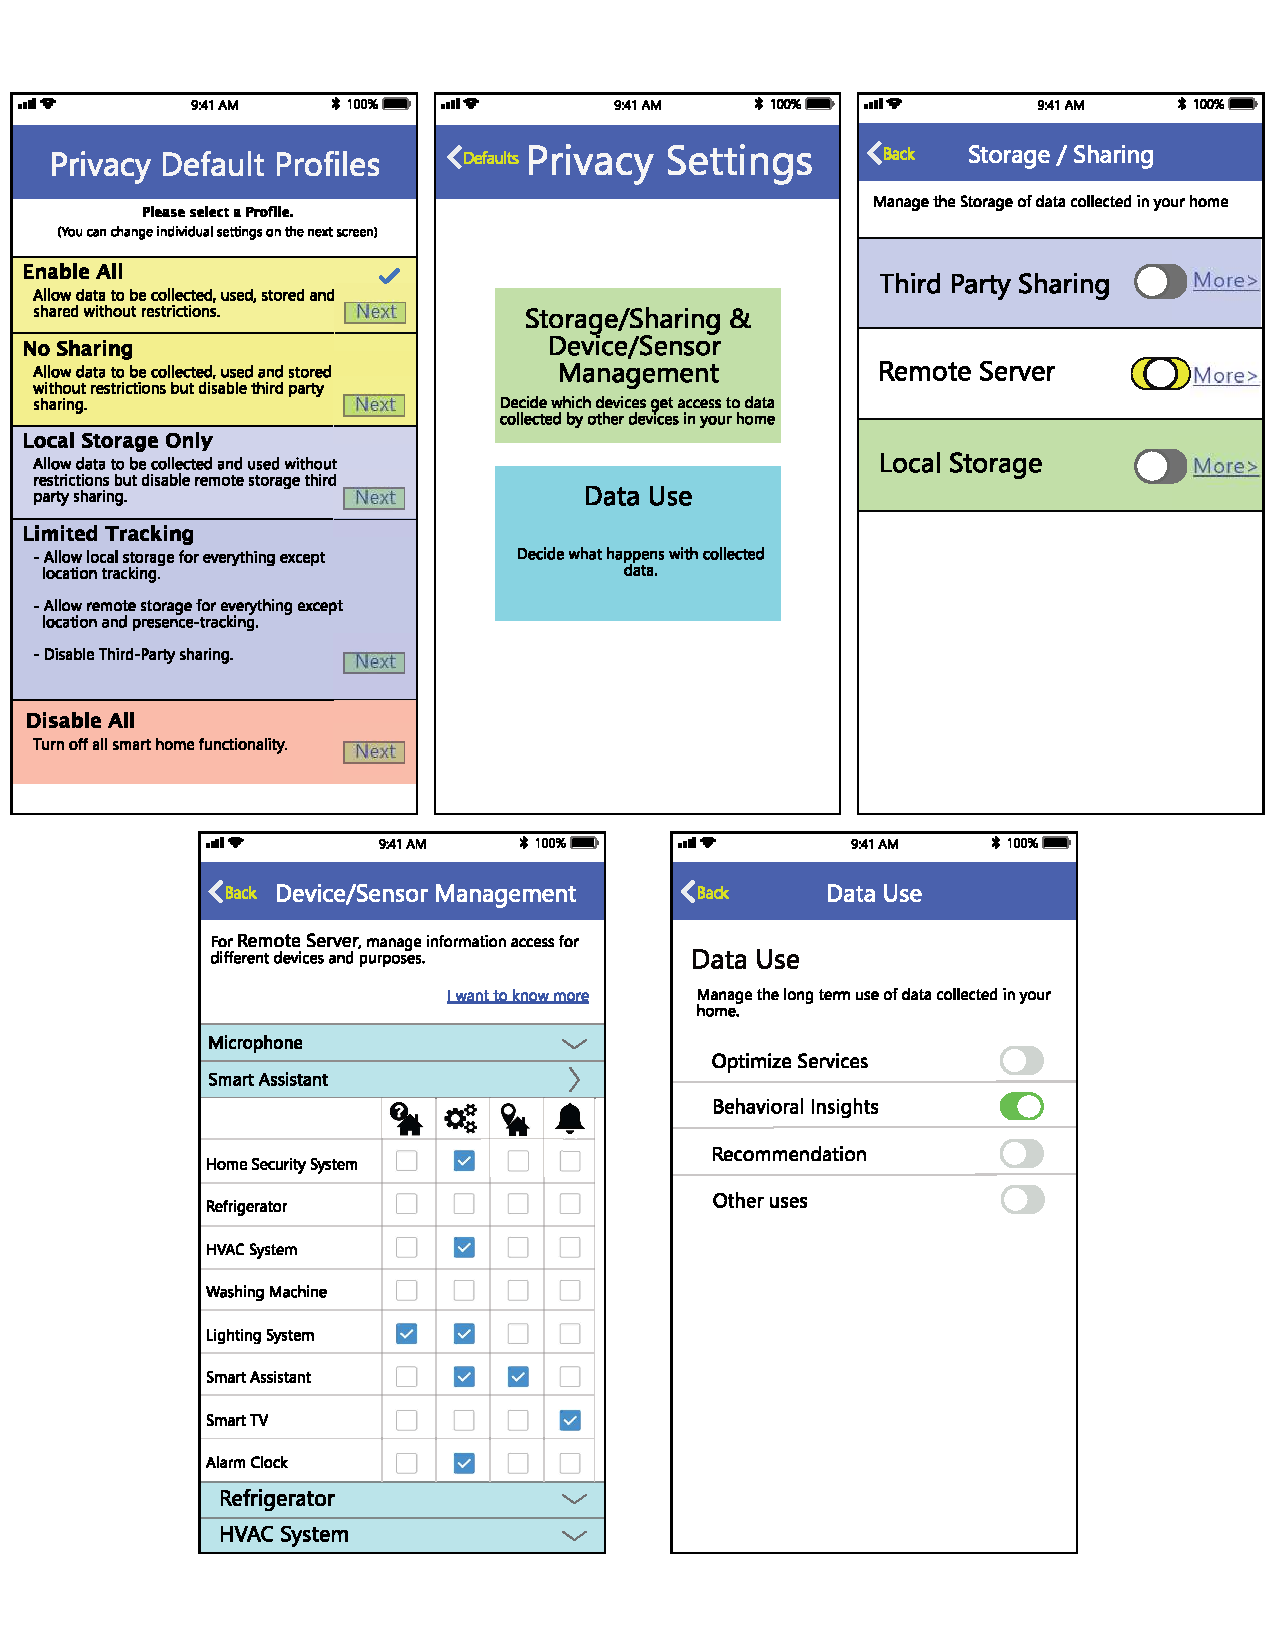
\includegraphics[width=0.8\textwidth]{figures/cluster_simple.pdf}
	\caption{Design for 5-Profile solution presented in Section~\ref{sec:fit_simple}. From top left, screen 1 is the profile selection page, screen 2 is the slightly altered landing page of our manual settings interface, screen 3 is the slightly altered Data Storage page, screen 4 (bottom left) is the Device/Sensor Management page, and screen 5 is the Data Use page.}
	\label{fig:cluster_simple}
\end{figure*}

\subsection{Interface for the 5-profile fit-based solution with an accuracy of 83.11\%}\label{sec:fit_complex}
The alternative machine learning solution presented in Figure~\ref{fig:fit_5_profile003} requires an additional interaction between the \emph{Storage} parameter and the \emph{Action} parameter. This requires us to slightly alter the interface again (see Figure~\ref{fig:cluster_complex}): 
\begin{itemize}
	\item \textbf{Screen 1:} The profile selection screen remains unchanged, with the exception that the `Local storage only' profile is replaced by the more complex `Local Storage \& No Recommendations' profile.
	\item \textbf{Screen 2:} After clicking `Next', users first get to set their sharing preferences for `local storage', `remote server' and `third party sharing' (\emph{Storage}). Each of these can independently be set to \emph{enabled} or \emph{disabled}, but users can also click on `More'.
	\item \textbf{Screen 3:} When users select `More', they are given the option to select either `Device/Sensor Management' or `Data Use'.
	\item \textbf{Screen 4:} When users select `Device/Sensor Management' they can manage \emph{Who-What-Purpose} combinations for that particular storage/sharing option.
	\item \textbf{Screen 5:} When users select `Data Use' they get to enable/disable the use of the collected data for various secondary purposes (\emph{Action}) for that particular storage/sharing option. 
\end{itemize}

\begin{figure*}
	\centering
	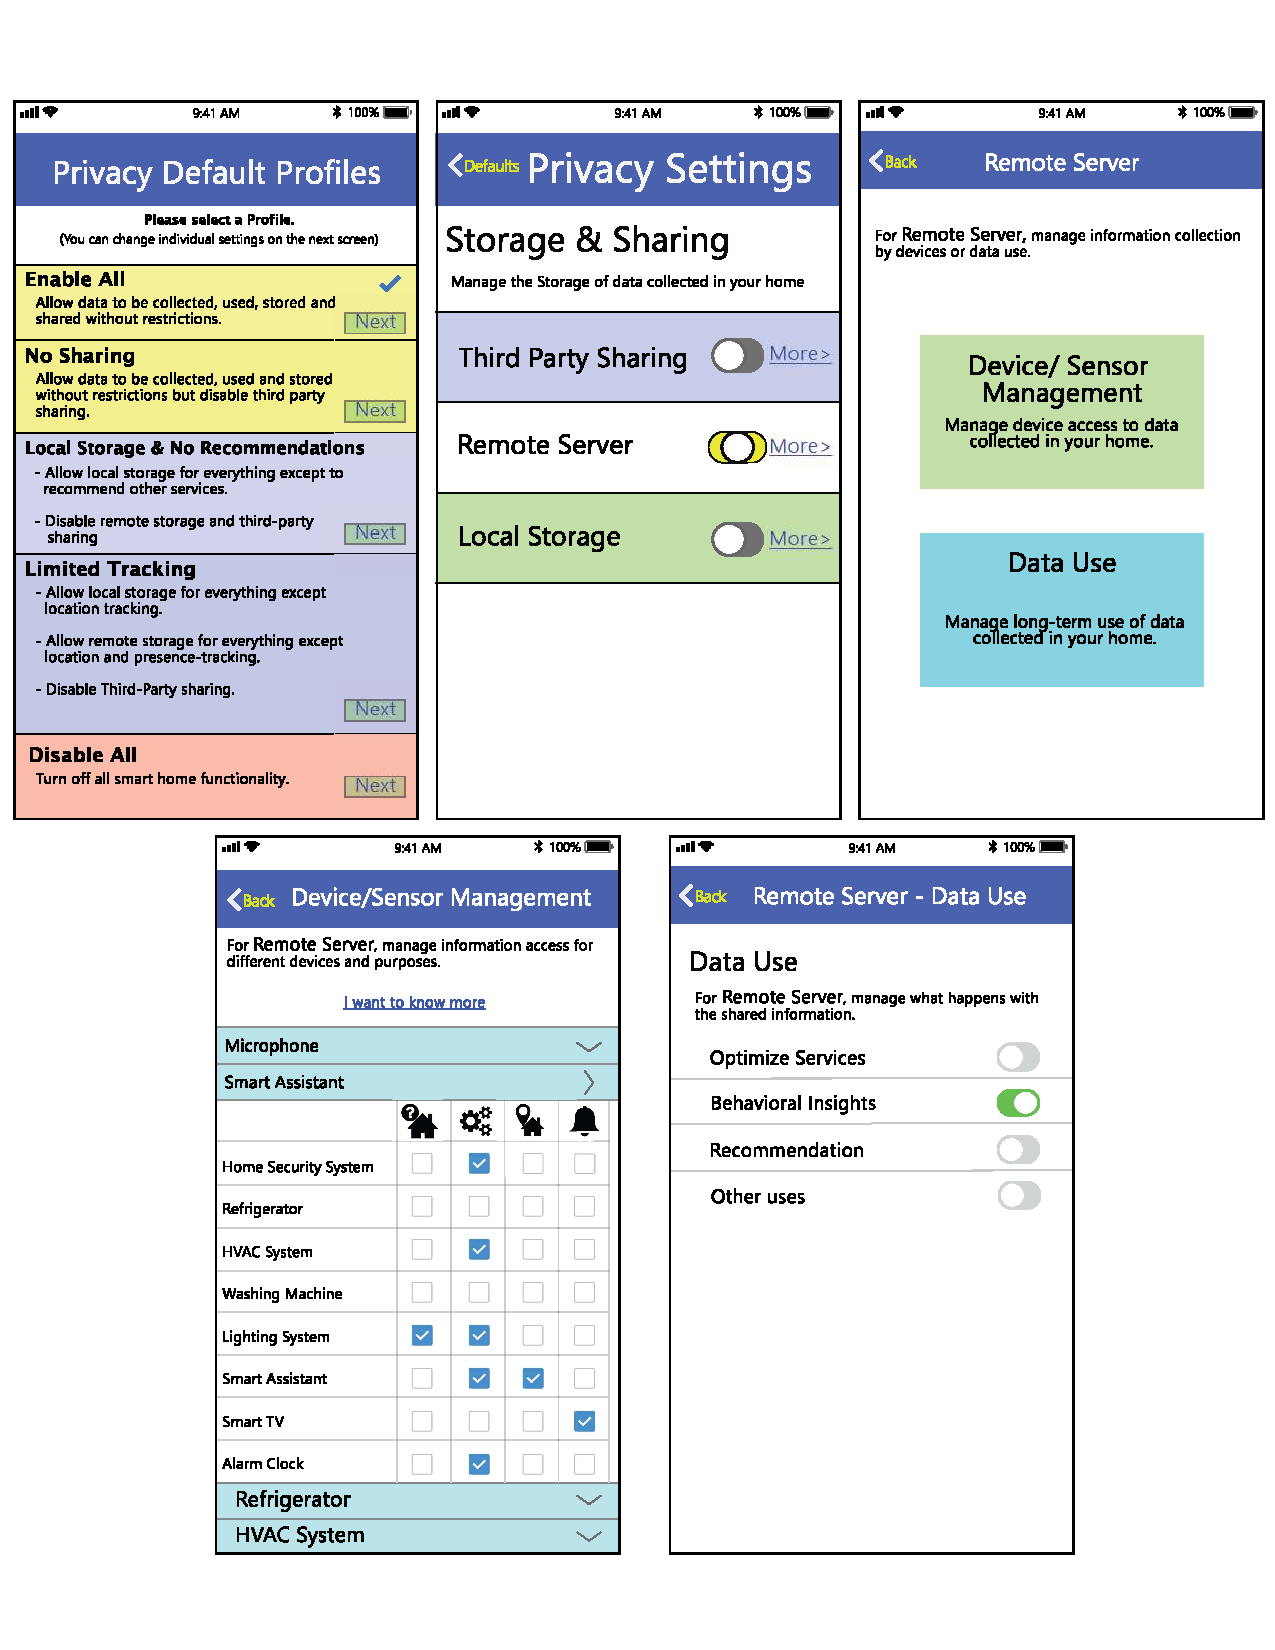
\includegraphics[width=0.8\textwidth]{figures/cluster_complex.pdf}
	\caption{Design for 5-Profile solution presented in Section~\ref{sec:fit_complex}. From top left, screen 1 is the profile selection page, screen 2 is the slightly altered Data Storage page, screen 3 follows the `More' button to offer access to screen 4 (bottom left, the Data Use page) and screen 5 (bottom right, the Device/Sensor Management page).}
	\label{fig:cluster_complex}
\end{figure*}

\subsection{Reflection on design complexity}
The interfaces presented in this section have an additional `layer' compared to the original interface presented in Section~\ref{sec:design_stat}. This additional layer makes setting the privacy settings manually more difficult, but it is necessary to accommodate the complexity of the smart profiles uncovered by our machine learning analysis. On the one hand, this demonstrates the value of developing a parsimonious machine learning model---the more accurate but more complex profiles that comprise some of the solutions in Section~\ref{sec:predict} are not only more difficult to explain to the user, they also contain more complex interactions between decision parameters, forcing the manual settings interface to become even more complex. A simple smart profile solution avoids such complexity in the interface. 

On the other hand, one should not over-simplify the profiles, lest they become overly generic and inaccurate in representing users' privacy preferences. Indeed, when we make our smart profile solutions more accurate, fewer users will need to make any manual adjustments at all, so we can allow some additional complexity in the interface.
	% !TeX root = disseration.tex
\chapter{Recommending Privacy Settings for Fitness IoT}\label{chapter:fitnessIoT}

\section{Introduction}\label{fitnessIntro}
In Chapter~\ref{chapter:generalIoT} and~\ref{chapter:householdIoT}, we have discussed how we apply the data-driven approach to the general/public IoT and household IoT contexts, respectively. We developed corresponding IoT privacy-setting interface prototypes that integrated with smart defaults/profiles by predicting users' privacy decisions. In this chapter, we present the work we did in the domain of fitness IoT. We further test the previously-developed data-driven approach to design privacy-setting interfaces for users of fitness IoT devices. Note that moving the context from general/public IoT to household IoT, now to fitness IoT, the context that we are focusing is becoming more narrow. The change of environment brought more challenge. For example, now for fitness IoT, there is no contextual scenario existing, which we focused on in Chapter~\ref{chapter:generalIoT} and~\ref{chapter:householdIoT}. Considering almost all the current fitness IoT devices require corresponding mobile Apps to be used together and the mobile Apps are usually the ones who are take charge of users' privacy information, we focus on the privacy permissions asked by the mobile Apps. In this Chapter, we first collect users permission decisions to the fitness IoT permissions. Then we apply our data-driven approach to classify users into groups based on their permission decisions, and create permission profiles for each groups. This allows new users to answer very few questions before getting a recommendation of a set of permission profile, which simplifies users' task of setting every permission for fitness IoT devices.

%As fitness-related data are persistently captured, stored, processed and shared by these devices and related services, the issue of privacy management is becoming increasingly urgent both for the user and the service, which has to respect privacy law, including the new European Union's General Data Protection Regulation (GDPR). This concerns all third parties that manage user data and has of course a major impact on personalization services.

%As of May 25, 2018, the European Union (EU) enforce the General Data Protection Regulation (GDPR)~\cite{ref:GDPR} which applies to the storage, processing and use of the subject's personal data from the third parties which may or may not have been established in the EU as long as they operate in an EU market or acess data of EU residents. It requires users to provide explicit consent to privacy options expressed by third parties. This results in a complex task for the users given the number of devices and applications which have to be read and processed specifically.

\section{Data Model}
As discussed in Section~\ref{fitnessIntro}, the mechanism that most modern fitness trackers use to guide their user to manage privacy settings is by asking users various permission questions. We first investigate the questions asked by mainstream fitness trackers, and then adapt those questions for the use of our data model in this study.

As shown in Figure~\ref{tab:trackerspermission}, we examined the permission questions asked by the mainstream fitness trackers (Fitbit, Garmin, Jawbone, and Misfit) and categorized these questions into 3 groups -- \textit{Smartphone Persmission}, \textit{In-app Requests}, and \textit{Fitness Data},.
 
\begin{figure*}
	\centering
	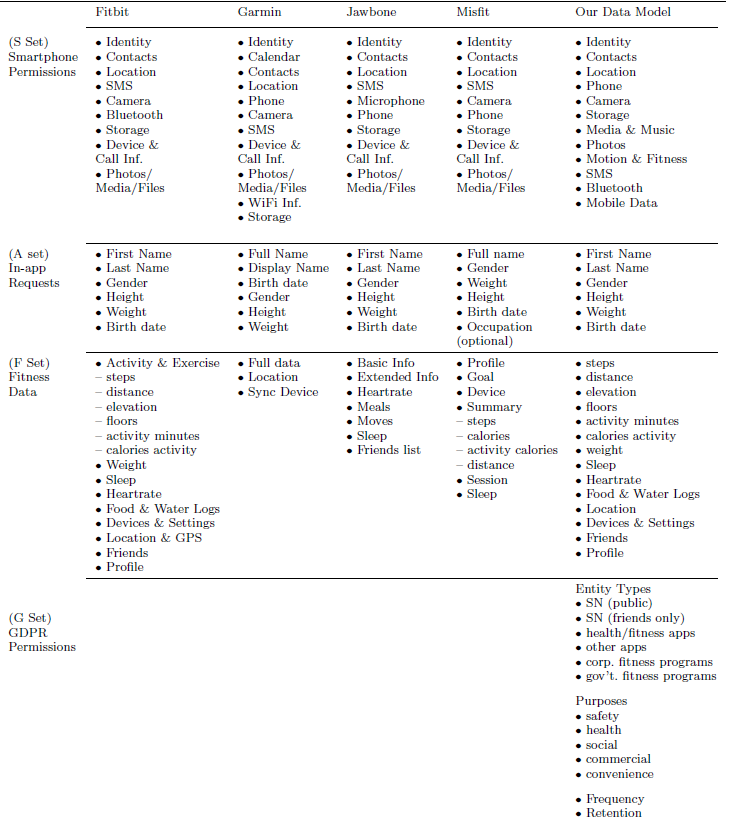
\includegraphics[width=\textwidth]{figures/fitnessCompare.png}
	\caption{Comparison of permissions asked by Fitness Trackers and the fitness IoT Data Model used for this study.}
	\label{tab:trackerspermission}
\end{figure*}

\subsection{Smartphone Permissions (S set)}
The first group of permissions are the smartphones permissions, which are requested during the installing or the first use of the mobile application. The requested smartphone permissions differs by the brands of the fitness trackers as well as the mobile Operation System of the smartphones. As shown in Figures~\ref{fig:iosS} and~\ref{fig:androidS}, even for the mobile application from the same manufacturer (Fitbit), the requested smartphone permissions are different between the iOS version and the Android version. We summarize all the requested smartphone permissions by popular brands of fitness trackers' mobile application across different mobile Operating Systems (i.e. iOS, Android, and Windows Mobile).

\begin{figure}
	\centering
	\begin{subfigure}[b]{0.48\linewidth}
		\centering
		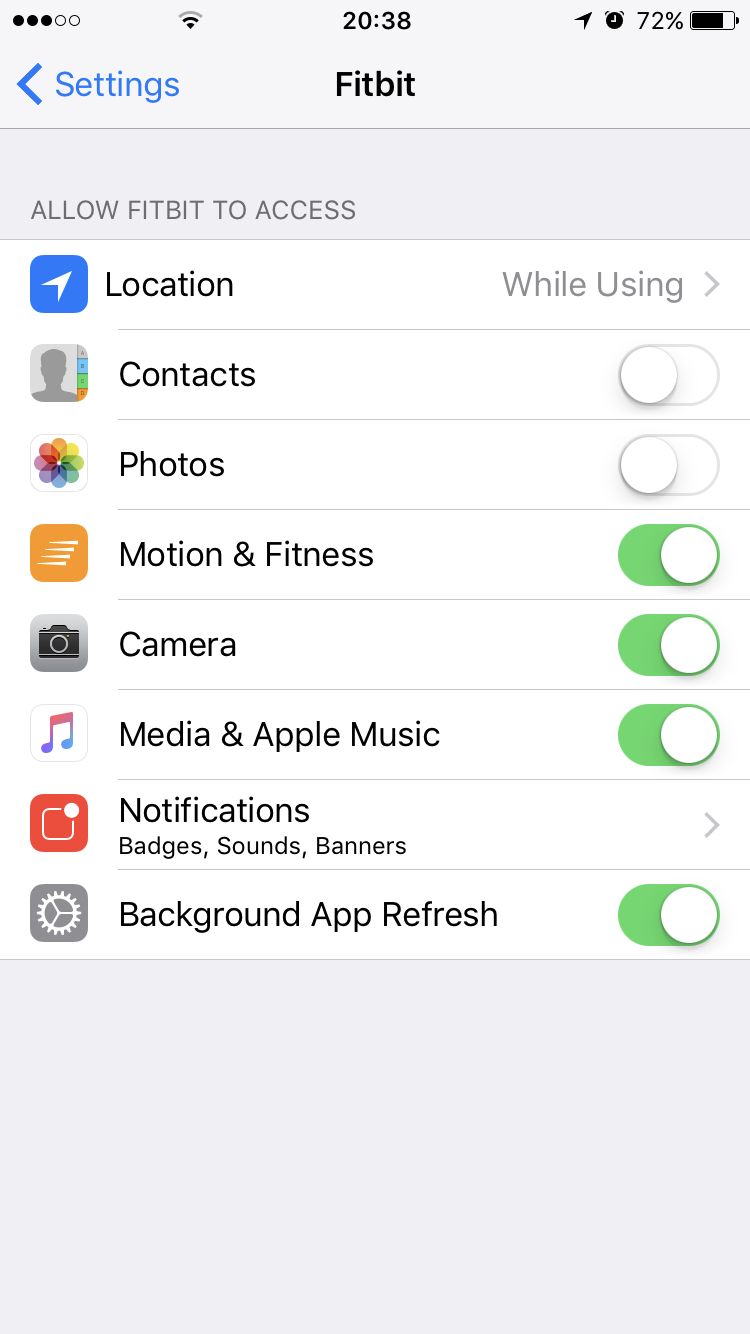
\includegraphics[width=120pt]{figures/ios.png}
		\caption{The interface of smartphone permissions of Fitbit iOS App}
		\label{fig:iosS}
	\end{subfigure}%
	\begin{subfigure}[b]{0.48\linewidth}
		\centering
		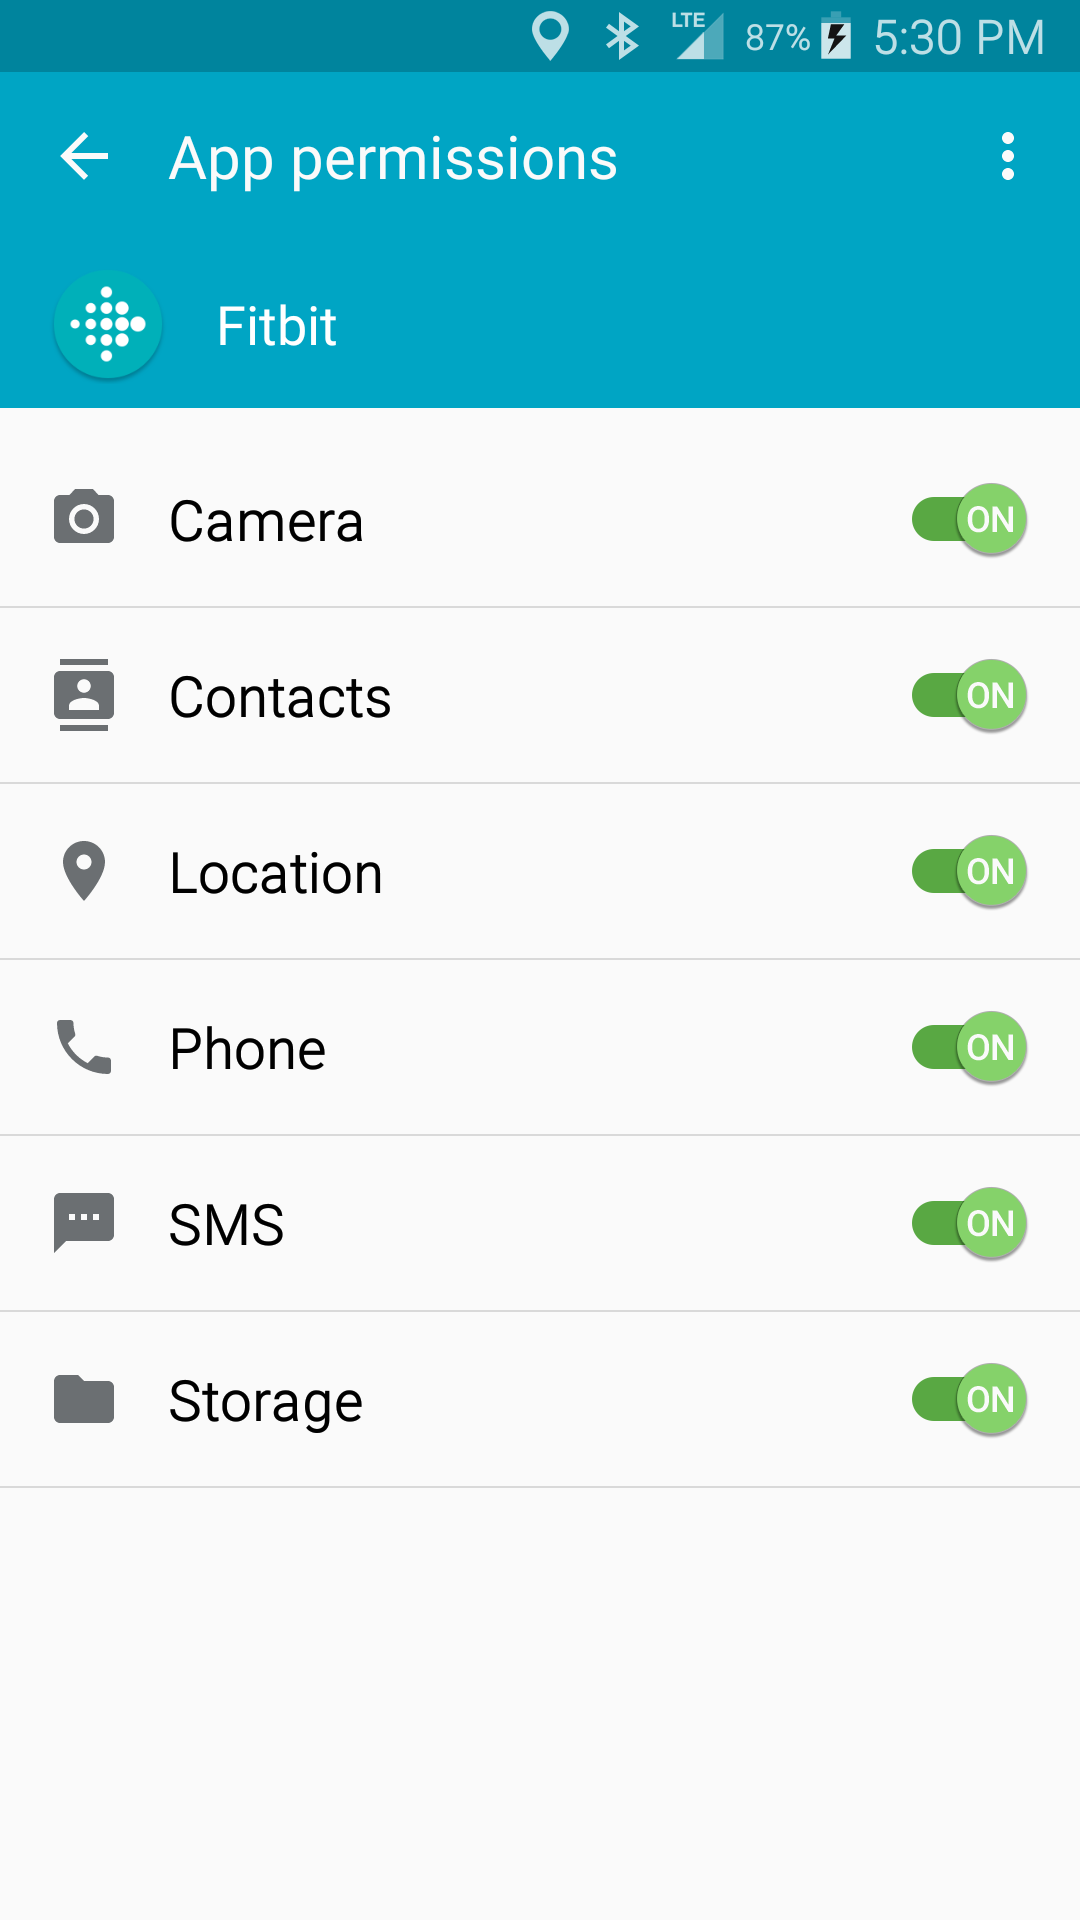
\includegraphics[width=120pt]{figures/android6.png}
		\caption{The interface of smartphone permissions of Fitbit Android App}
		\label{fig:androidS}
	\end{subfigure}
	\caption{Interface examples of Smartphone Permissions requests for Fitbit trackers (S set)}
	%\caption{\subref{fig:iosS} shows Figure~1 and~\subref{fig:androidS} shows Figure~2.}
\end{figure}

\subsection{In-App Requests (A set)}
Fitness tracks also intend to collect user's data in their mobile applications. For example, Fitbit asks users to provide their \textit{First Name}, \textit{Last Name}, \textit{Gender}, \textit{Height}, \textit{Weight}, \textit{Birth Date}, as shown in Figure~\ref{fig:fitbitA} when signing up an account during the first-time using the mobile App. Note that these data are mandatory for all fitness trackers in Figure~\ref{tab:trackerspermission}; the only optional piece of information is Misfit's request on users' occupation. Figure~\ref{fig:fitbitA} shows the \emph{A set} for the Fitbit app (other apps are similar).
\begin{figure}
	\centering
	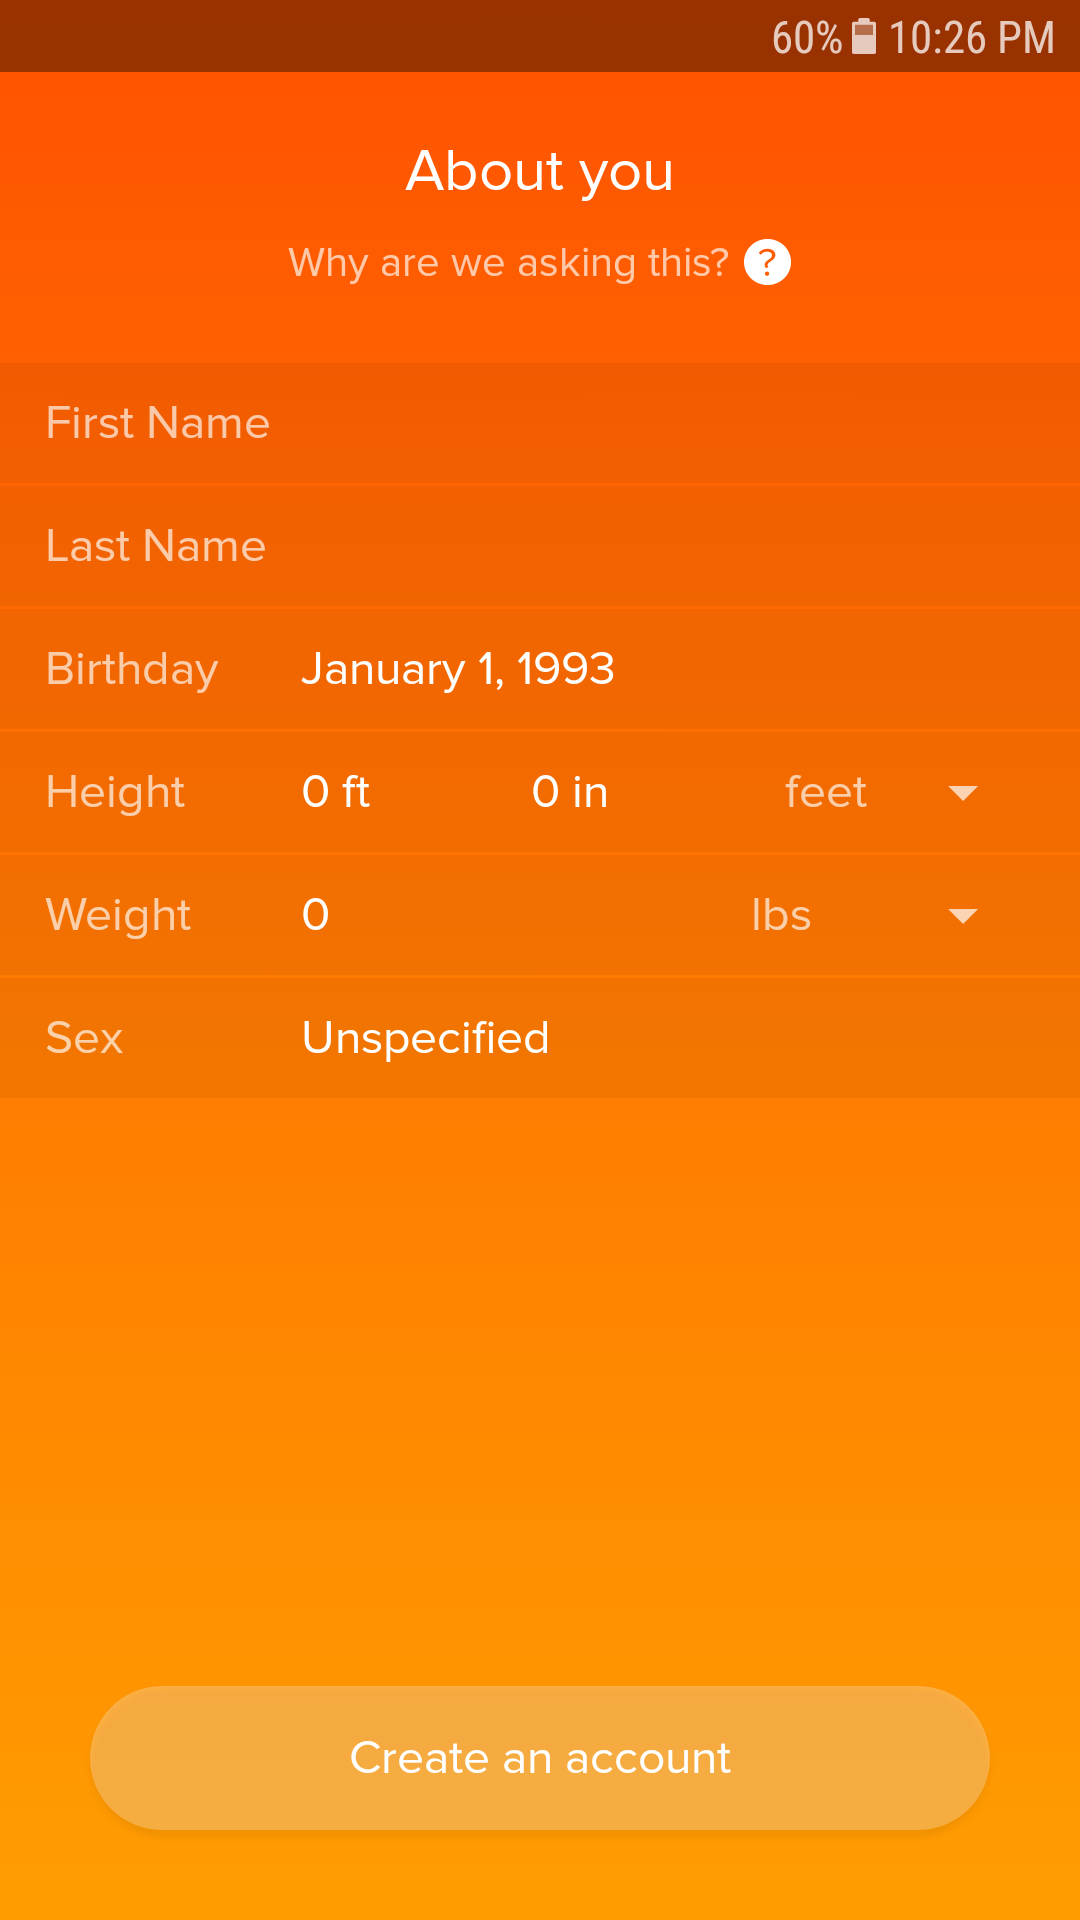
\includegraphics[width=0.2\textheight]{figures/Aset.png}
	\caption{Interface example of In-App Permissions requests in Fitbit Android App (A set)}
	\label{fig:fitbitA}
\end{figure}

\subsection{Fitness Data Permissions (F set)}
\label{sec:fset}
F set contains fitness-related data that is either automatically collected by the fitness tracker or manually input by the users, such as food and water logs, friend list. As shown in Figure~\ref{tab:trackerspermission}, we follow Fitbit's permission model for F set but give users more fine-grained control over \textit{Activity and Exercise} data by breaking these permissions down into steps, distance, elevation, floors, activity minutes, and calories activity. A total of 14 permissions are included in the F set for our study. 

%NEW
%new: according to Prof. Bart, explain the F-G connection
%Note that the F set permissions are repeated for \emph{each additional TP} that requests access to this data. As such, these permissions are not for the native app of the fitness tracker, but for other TP apps that the user desires to use and allow access to her/his fitness tracking data. In this study, instead of taking into account individual third parties, we use the PPIoT \textit{EntityType}, discussed in Section \ref{sec:ppiot}, to investigate which group category of TP apps (namely ``who") the user prefers to share with. This parameter has been shown to be important in determining users' privacy settings~\cite{lee2017privacy}. Since Entity Types are intimately related to GDPR-based requirements, these permissions are included in the G set. 

\subsection{GDPR-based Permissions (G set)}
\label{sec:gset}
As of May 25, 2018, the European Union (EU) enforce the General Data Protection Regulation (GDPR)~\cite{ref:GDPR} which applies to the storage, processing and use of the subject's personal data from the third parties which may or may not have been established in the EU as long as they operate in an EU market or acess data of EU residents. It requires users to provide explicit consent to privacy options expressed by third parties.
The G set includes permissions that are based on GDPR requirements. The purpose of data collection, \textit{hasReason}, includes \textit{safety}, \textit{health}, \textit{social}, \textit{commercial} and \textit{convenience}. The frequency of data access, \textit{hasPersistence}, includes \textit{continuous access}, \textit{continuous access but only when using the app}, and \textit{separate permissions for each workout}. For the retention period of collected data, \textit{hasMaxRetentionPeriod}, permissions include \textit{retain until no longer necessary}, \textit{retain until the app is uninstalled}, and \textit{retain indefinitely}. We did not include the \textit{hasMethod} property since it involves technical background.

The types of third parties  (instances of \textit{EntityType}) that can request access to the user's Fitness data include \textit{health/fitness apps}, \textit{Social Network (SN) apps} (\textit{public} or \textit{friends} only), \textit{other apps on the user's phone}, and \textit{corporate} and \textit{government fitness programs}.



%\subsection{A Conundrum of Settings}
%
%We note that Fitbit asks for a staggering total of 24 permissions across the S, A, and F data sets. Our data model, which takes a superset of permissions asked by all four fitness trackers, more granular \textit{Activity and Exercise} data, and the additional G set, includes 45 permissions in total. Moreover, if the user wants to share their fitness data (F set) with one or more additional health or fitness tracking apps, the permissions for this must be decided upon for each additional TP individually. 
%
%Most current fitness tracker apps do not ask these permissions in a very clear manner, and the settings are often hard to find in case the user wants to change them. That said, even with a more usable UI for making these settings the sheer number of them is arguably a significant burden to the user and cause of possible errors. This is why we advocate the use of semi-automated interactive \emph{privacy recommendations} to partially relieve users' burden of setting each of these individual permissions and meanwhile maintain the control on privacy preferences.

\section{Dataset}
The dataset we use in this study was collected by my colleague Odnan. 310 participants were asked to set up a new account using a fitness tracker mobile App similar to Fitbit. They were then asked the 4 groups of questions that we discussed in our data model. For each question, the answer will be either ``Allow" or ``Deny", meaning the participants are either willing to provide information for that permission or not. After answering these questions, participants were then asked to fill our a survey questionnaire measuring their privacy-related attitudes (i.e. Trust, Privacy concerns, Perceived surveillance and intrusion, and Concerns about the secondary use of personal information), the negotiability of their privacy settings, their social behaviour (social influence and sociability), exercise tendencies (a proxy for their attitude and knowledge about fitness tracking), and demographic information.
%To conduct the data collection, a mobile fitness application mock-up, named \textit{FitPro} was developed. FitPro systematically asked for all of the permissions in the Data Model for Fitness IoT that we defined in Section~\ref{sec:trackers}. Participants were asked to set up an new account by providing their information. All the questions at this stage are organized according to our data model discussed in previous section, including 1) In-app permissions, 2) Smartphone permissions, 3) Fitness data permissions, and 4) GDPR-based permissions. After providing answers to these questions, participants were asked to fill our a survey questionnaire. We aimed to measure the users' privacy-related attitudes (trust, privacy concerns, perceived surveillance and intrusion, and concerns about the secondary use of personal information), the negotiability of their privacy settings, their social behaviour (social influence and sociability), exercise tendencies (a proxy for their attitude and knowledge about fitness tracking), and demographic information. The questionnaire is shown in Appendix.

%A total number of 310 participants were recruited through Amazon Mechanical Turk. After data preprocessing, 295 user samples were utilized. We asked people to only participate if they were active Fitbit users\footnote{We restricted our study to Fitbit users rather than users of any fitness trackers to make sure that our sample had a more homogeneous existing experience with fitness permission-setting interfaces.}, and checked this requirement by asking participants to enter the initial and last few digits of their Fitibit serial number. The participants consisted  of 34.2\% males and 65.8\% females, had mean age of 35, and were generally highly educated (62\% had at least a bachelor's degree). We restricted our study to fitness tracker users to detect the real preferences of target users.

%\section{Data Analysis}
%In this section, we present our data analysis on the dataset. 
As shown in Figure~\ref{fig:mean}, participants intend to have a higher disclose rate for their demographics information (A set), which is in line with the results of other studies~\cite{knijnenburg2013helping}.

For the smartphone permissions (S set), participants are more likely to allow motion, location, bluetooth, and mobile data, which are usually the minimum permissions required for a fitness mobile App to work. In S set, the access to contacts and photos are the least allowed permissions.

Regarding the G set, participants seem most open to data collection for health (the main purpose of a fitness tracker) and safety (another popular purpose often advertised by the manufacturers). On the other hand, users are less likely to agree to data collection with an indefinite retention period, and they prefer not to share data with government fitness programs or publicly on social media. 

\begin{figure}
	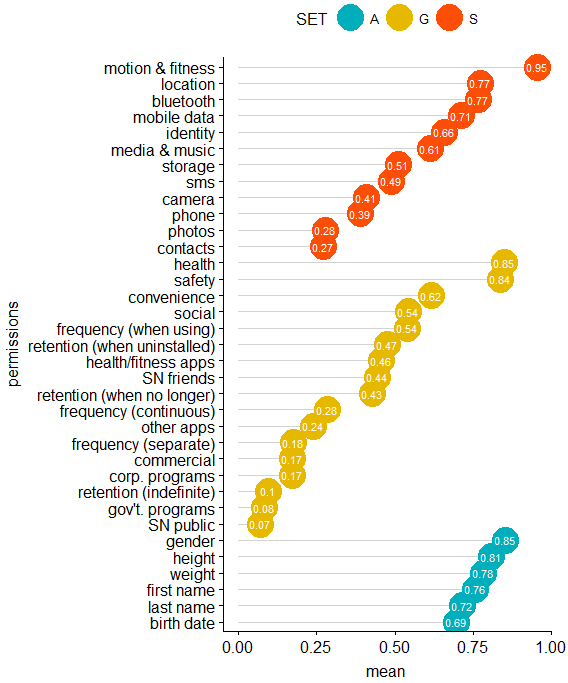
\includegraphics[width=\linewidth]{figures/sum2.png}
	\caption{Average values of each privacy permissions (1-allow, 0-deny).}
	\label{fig:mean}      
\end{figure}
%
%\begin{figure}[ht]
%	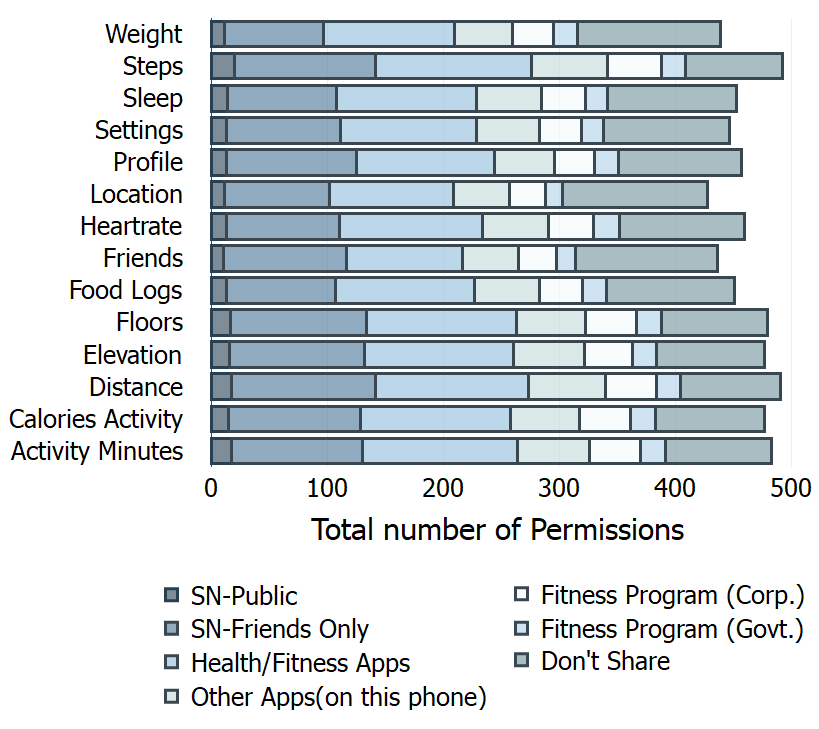
\includegraphics[width=0.98\linewidth]{figures/fdata6.png}
%	\caption{Distribution of fitness data (F set) with respect to different Entity Types (G set).}
%	\label{fig:fdata}      
%\end{figure}

%ODNAN: edited a little to connect F-G entity types
%We do not show the fitness data (F set) in Figure~\ref{fig:mean} because the permissions for these data are requested for multiple entity types of the G set, as discussed in Section~\ref{sec:fset}. Hence, we present these data in Figure~\ref{fig:fdata} instead, showing each permission for each GDPR \textit{EntityType}. 
%%Participants are likely to share their Fitness data (as 40.33\% of the respondents have already shared them in real life scenario). What differs is their perception for the receiving entity of the data. Figure~\ref{fig:fdata} shows the distribution of permissions for different entity types. 
%Users are more likely to give permission to their friends on social networks and to other health/fitness apps, and they are less likely to give permission to share their data with government fitness programs or publicly on social media. As for various data types, steps are shared most openly, while location, friends, and weight are shared less openly.
%
%Upon further inspection, we note that participants tend to share either (almost) all or (almost) none of fitness data with an entity. This suggests that Fitness data permissions are more likely to be influenced by the receiver (``who'') rather than the specific data item (``what'').
%%NEW
%%NEW:ODNAN: i am trying to remind again the reader here that entity type is from G and is split from F 
%As discussed in Section \ref{sec:ppiot}, these ``who'' parameters are instances of the GDPR \textit{EntityType}. Therefore, we expect that clustering F permissions should provide a unanimous deny/share for all items, while clustering G permissions should provide more nuanced clusters of different entity types receiving the data specified in the F set.


\section{Predicting users' Preference (partial original work)}
We predict participants' \textit{allow}/\textit{deny} decision using machine learning methods. Our dataset shows considerable variability between participants' privacy preferences---a finding that is broadly reflected in the privacy literature~\cite{knijnenburg2013dimensionality}. Using clustering, one can capture the preferences of various users with a higher level of accuracy. Hence, the goal of this section is to find a concise set of profiles, clusters, that can represent the variability of the permission settings among our study participants. 

We cluster participants' permissions with Weka\footnote{\url{https://www.cs.waikato.ac.nz/ml/weka/}} using the K-modes clustering algorithm with default settings. The K-modes algorithm follows the same principles as the more common K-means algorithm, but it is more suitable for the nominal variables in our dataset.

%Privacy-setting Profiles are then generated from each cluster. The advantage of this method is that users can set up all their privacy settings by one or few clicks. However, in the other hand, there are some drawbacks about this approach. Advanced users may still need to check each of the settings and change what they need. And the profile provided will be long since all the settings from four different sets are presented in a single profile. Moreover, assume we cluster the users into $n$ clusters, the naive method will only provide $n$ possible profile recommendations to the users. However, if we generate profiles from each of the four datasets (A, F, S, and G), a total number of $n^4$ different combinations of profiles can be recommended, providing a more fine-grained privacy-setting control to the users than the naive method. In the following, we will discuss our method that generates set-based profiles for each of the four datasets, called \textit{sub-profile}.

\begin{figure*}[ht]
	\centering
	\begin{subfigure}[b]{0.4\linewidth}
		\centering
		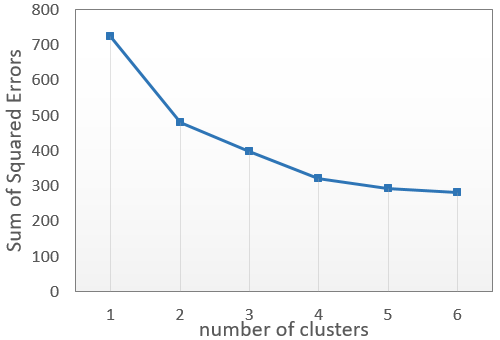
\includegraphics[width=150pt]{figures/Scluster_new4.png}
		\caption{S dataset}
		\label{fig:numS}
	\end{subfigure}
	\begin{subfigure}[b]{0.4\linewidth}
		\centering
		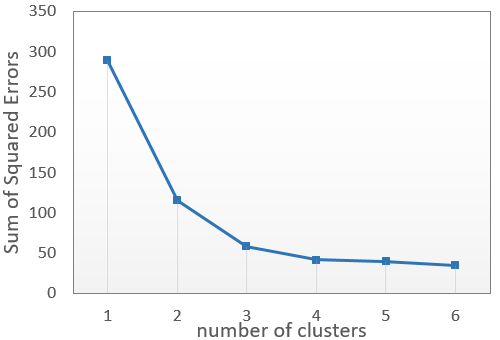
\includegraphics[width=150pt]{figures/Acluster_new4.png}
		\caption{A dataset}
		\label{fig:numA}
	\end{subfigure}
	\begin{subfigure}[b]{0.4\linewidth}
		\centering
		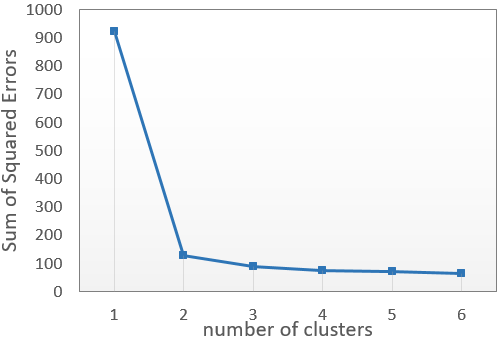
\includegraphics[width=150pt]{figures/Fcluster_new4.png}
		\caption{F dataset}
		\label{fig:numF}
	\end{subfigure}
	\begin{subfigure}[b]{0.4\linewidth}
		\centering
		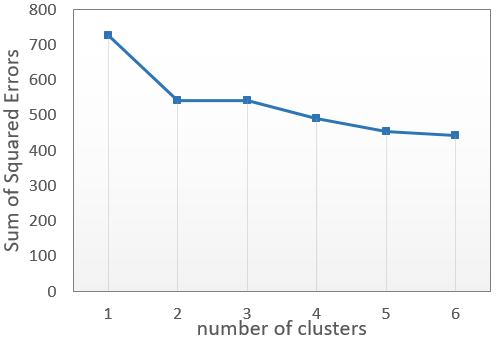
\includegraphics[width=150pt]{figures/Gcluster_new4.png}
		\caption{G dataset}
		\label{fig:numG}
	\end{subfigure}
	\caption{Evaluation of different numbers of clusters for each set.}
	\label{fig:cluster_evaluation}
\end{figure*}


\subsection{Overall Prediction}
In our first clustering attempt we tried to find a set of profiles by clustering the full dataset, including the A, F, S, and G subsets.
A drawback of this method is that, assume we cluster the users into $n$ clusters, this  method will  only provide $n$ possible profiles to be used for recommendations to the users. A further drawback of clustering based on the full set of 45 permissions is that it has high error rates (e.g., the sum of squared error for the viable 4-cluster solution is 1435 and 1688 for 2-cluster solution). In addition, the profile provided will be complicated since all the settings from four different sets are presented in a single profile, making it difficult to explain to the users.

If we instead generate a separate set of $n$ ``subprofiles'' for each of the four datasets (A, F, S, and G), $n^4$  different combinations of profiles can be used for recommendation, providing finer-grained privacy-setting controls to the users compared to clustering the full set. In addition, error rates are lower when clustering each set separately, as shown in Figure \ref{fig:cluster_evaluation}. For example, with only 2 clusters per set, the sum of squared error reduces to 1277 (a 24.3\% reduction). %BART: please enter this number %ODNAN: 1277 is the total sum of the S F A G sum of squared error
An additional benefit is that the profiles for each set can be investigated in more detail. 


%new addition: as suggested by Prof. Bart
In our dataset the fitness data permissions (F set) are specified repeatedly for each Entity Type (part of the G set). We tried to cluster these combinations, taking into account all 98 features (i.e., 14 fitness data per 7 entity types). This analysis resulted in two profiles: one that had ``allow all'' for health and SN public entities (and ``deny all'' for all other entities), and one that had``deny all'' for all entities. This means that: a) very similar results can be obtained by considering the fitness data permissions separately from the Entity Type, and b) as expected, the ``who'' parameter (Entity Type) is more important than the ``what'' parameter (fitness data permissions). 

In the following, we will discuss our method that generates subprofiles for each of the four datasets.


\subsection{2-Cluster Solution}

We first investigate the optimal number of clusters by running the K-modes algorithm for 1-6 clusters with a 70/30 train/test ratio, using the sum of squared errors of the test set for evaluation. The results are shown in Figure~\ref{fig:cluster_evaluation}. Using the elbow method~\cite{kodinariya2013review}, we conclude that 2 is the optimal number of clusters for each dataset\footnote{We obtain similar results using other clustering algorithms, such as Hierarchical Clustering.}. 
%More importantly, the F set shows a distinctive 2-cluster solution as shown in Figure~\ref{figures/fig:fgraph}, which is consistent to the reasons mentioned on Section~\ref{sec:analysis} about the requesting entity type. It is also consistent with the results in~\cite{lee2017privacy}, where the identity of the information requester (\textit{who} context) is an important determinant of people’s privacy decisions, thus in turn results in unanimous allow or deny for the fitness data permissions.
%BART: didn't you split this data by recipient type?



The final cluster centroids of the 2-cluster solution for each dataset are shown in Figure~\ref{fig:privacy_profiles}, together with the results of the 1-cluster solution. %BART: to avoid confusion, we should not call this "full data" but rather "single cluster" %ODNAN: OK
We describe the subprofiles of each set in the subsections below.

%BART: Should we provide accuracies here?
%there is no accuracy yet, instead, the error rates of the clusters which are already in the Figure 7, these are their respective centroid
\begin{figure}
	\centering
	\begin{subfigure}[b]{0.4\linewidth}
		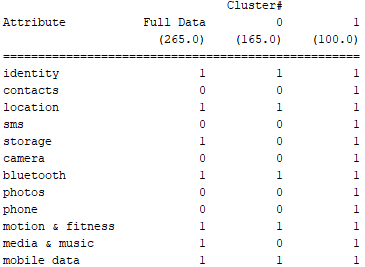
\includegraphics[width=0.85\linewidth]{figures/S_new2.png}
		\caption{S dataset}
		\label{fig:scluster}
	\end{subfigure}
	\begin{subfigure}[b]{0.4\linewidth}
		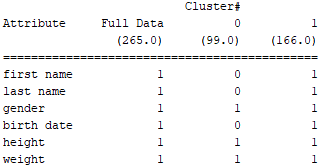
\includegraphics[width=0.85\linewidth]{figures/A_new2.png}
		\caption{A dataset}
		\label{fig:acluster}
	\end{subfigure}
	\begin{subfigure}[b]{0.4\linewidth}
		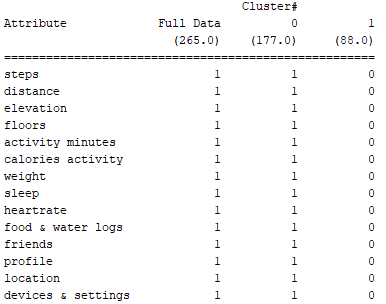
\includegraphics[width=0.85\linewidth]{figures/F_new2.png}
		\caption{F dataset}
		\label{fig:fcluster}
	\end{subfigure}
	\begin{subfigure}[b]{0.4\linewidth}
		\includegraphics[width=0.85\linewidth]{figures/G_new2.png}
		\caption{G dataset}
		\label{fig:gcluster}
	\end{subfigure} 
	\caption{Privacy profiles from the two clustering methods:  1-cluster results (full data) and 2-clusters results (privacy subprofiles)  for each dataset(allow=1, deny=0, except for frequency \& retention)}
	\label{fig:privacy_profiles}
\end{figure}


\subsubsection{The \textit{S} Set}
\begin{itemize}
	\item \textbf{Minimal} (cluster 0): this subprofile allows the minimum permissions needed to effectively run a fitness app. This includes identity, location, bluetooth, motion \& fitness, and mobile data permissions.
	
	\item \textbf{Unconcerned} (cluster 1): this subprofile allows all permissions in this dataset.
\end{itemize}

\subsubsection{The \textit{A} Set}
\begin{itemize}
	\item \textbf{Anonymous} (cluster 0): this subprofile shares only users' gender, height and weight information but not their birth date or first and last name.
	
	\item \textbf{Unconcerned} (cluster 1): this subprofile shares all data requested in this dataset.
\end{itemize}

\subsubsection{The \textit{F} Set}
\begin{itemize}
	\item \textbf{Unconcerned} (cluster 0): this subprofile shares all fitness data with third parties.
	
	\item \textbf{Strict} (cluster 1): this subprofile does not share any fitness data with third parties.
\end{itemize}

%The unanimous deny/allow permission behavior of F set is consistent with the reason provided on Section~\ref{sec:analysis} regarding the effect of the requesting entity type.
%BART: this just calls attention to the fact that you didn't split this data by recipient type...

\subsubsection{The \textit{G} Set}
\begin{itemize}
	\item \textbf{Socially-active} (cluster 0): this subprofile shares data with health/fitness apps and social network friends, but not with other recipients. %BART: Again, shouldn't the recipient be part of the F-set rather than the G-set? This is very confusing!! 
	%ODNAN:the explanation why entity type is for the G set is explained in the GDPR section, moreover, GDPR permissions are not yet part of today's scenario, and that is also true for the entity type 
	%ODNAN: ALready resolved on the email thread
	Sharing is allowed for health, safety, and social purposes but not for commercial purposes.
	
	\item \textbf{Health-focused} (cluster 1): this subprofile does not allow sharing with any third parties. Sharing is allowed only for health and safety purposes. 
\end{itemize}

\section{Profile Prediction (original work)}
\label{sec:prediction}


Now that we have identified two privacy ``subprofiles'' per dataset, the next step is to find predictors for the profiles and predict which subprofiles each participant belongs to.  

Recommender systems usually ask users to evaluate a few items before giving recommendations regarding all remaining items. Likewise, in our system, we might be able to identify certain permission items inside each privacy subprofile that---when answered by the user---could drive the prediction. Since the items are the permission preferences included in the subprofiles, we define this as the ``direct predicition'' approach.

Additionally, we also explored whether the items from our questionnaire could drive the predicition. Since these items are not part of the privacy subprofiles, we define this as the ``indirect prediction'' approach. For each approach and for each subset of data (S, A, F, and G sets), we develop decision trees that will enable us to predict which subprofile best describes a user. The trees contain the subprofile items (direct prediction) or questionnaire items (indirect prediction) that can be asked to classify each user into their correct subprofile.

We developed our decision trees using the J48 decision tree learning algorithm and evaluated the resulting decision tree using cross validation.%J48 is an efficient and widely used decision tree algorithm that can be used for classification~\cite{patil2013performance}. Previous work shows the effectiveness of this approach to predict privacy settings within each cluster~\cite{bahirat2018data}; here we take the opposite approach and use it to predict cluster assignments instead. In our approach, the J48 algorithm extracts the permission items (for the direct prediction) or questionnaire items (for the indirect prediction) that classify a new user into the correct subprofile with the highest possible accuracy.

%The evaluation of all developed J48 trees was performed using k-fold cross validation. %\cite{kohavi1995study}. 


% will we include all the cross-validation results?
%The full details of the evaluation are shown in the Appendix~\ref{sec:appendix}.


\subsection{Direct Prediction Questions}
\label{sec:direct}

In our direct prediction approach, the aim is to ask users to answer certain permission items from each subset as a means to classify them into the correct subprofile (thereby providing a recommendation for the remaining items in that subset). For this approach, we thus classify users using the items in the subset as predictors. 

Our results for this approach are reported in Figure~\ref{fig:tree1}. It shows for each subset the question that best classifies our study participants into the correct subprofile.

\begin{figure}
	\centering
	\begin{subfigure}[b]{0.4\linewidth}
		\includegraphics[width=0.5\linewidth]{figures/s_tree1new.png}
		\label{fig:stree1}
		\caption{S set (86.42\%)}
	\end{subfigure}
	\begin{subfigure}[b]{0.4\linewidth}
		\includegraphics[width=0.5\linewidth]{figures/a_tree1new.png}
		\label{fig:atree1}
		\caption{A set (95.85\%)}
	\end{subfigure}
	\begin{subfigure}[b]{0.4\linewidth}
		\includegraphics[width=0.5\linewidth]{figures/f_tree1new.png}
		\label{fig:ftree1}
		\caption{F set (97.74\%)}
	\end{subfigure}	
 	\begin{subfigure}[b]{0.4\linewidth}
	 	\includegraphics[width=0.5\linewidth]{figures/g_tree1new.png}
	 	\label{fig:gtree1}
	 \caption{G set (82.26\%)}
	\end{subfigure}

	\caption{The permission drivers for the privacy subprofiles and their respective prediction accuracies.}
	\label{fig:tree1}
\end{figure} 


When running tree-based algorithms, a trade-off has to be made between the parsimony and the accuracy of the solution. Parsimony prevents over-fitting and promotes fairness and can be accomplished by pruning the decision trees. In our study, while multi-item trees may provide better predictions, the increase in accuracy is not significant compared to the single-item trees presented in Figure~\ref{fig:tree1}. These single-item solutions already obtained a high accuracy, and their parsimony prevents over-fitting and minimizes the number of questions that will need to be asked to the users in order to provide them accurate recommendations. The resulting solution involves a 4-question input sequence---one question for each subset. 

For the S set, the Photo permission is the best subprofile predictor. This is one of the least-shared permissions (see Figure~\ref{fig:mean}), and 94\% of participants who give this permission are correctly classified into the ``Unconcerned'' subprofile, while 83\% of participants who do not give this permission are correctly classified into the ``Minimal'' subprofile. 

For the A set, First name is the best predictor. Again, 94\% of participants who share their first name are correctly classified into the ``Unconcerned'' subprofile, while 98\% of participants who do not share their first name are correctly classified into the ``Anonymous'' subprofile.

For the F set, Activity minutes permission is the best predictor. This is one of the most-shared permissions. 97\% of participants who give this permission are correctly classified into the ``Unconcerned'' subprofile, while 100\% of participants who do not give this permission are correctly classified into the ``Strict'' subprofile.

Finally, for the G set, the best predictor is whether the participants allows data collection for Social purposes. If so, participants are correctly classified into the ``Socially active'' subprofile with 84\% accuracy, otherwise they are classified into the ``Health-focused'' subprofile with 80\% accuracy.


\subsection{Indirect Prediction Questions}

A similar procedure was applied to the questionnaire data concerning the following categories of user traits: privacy attitude, social behavior, negotiability, exercise tendencies and  user demographics (cf. Table \ref{tab:questionnaire} in Appendix).
As will be shown below, the indirect prediction approach has a lower accuracy than the direct approach presented in Section~\ref{sec:direct}. This is expected since the questionnaire items about user traits have no direct relationship with the permission settings in the privacy profiles.
These results are still interesting, though, since they allow the user to avoid making any specific privacy settings. Moreover, the resulting predictors show interesting semantic relationships with the datasets they predict. We discuss these results in more detail below.

\subsubsection{Privacy Attitudes}

We first attempted to use privacy attitudes as predictors of users' subprofiles. The resulting trees for this indirect prediction are shown in Figure~\ref{fig:tree2}.


\begin{figure}
	\centering
	\begin{subfigure}[b]{0.4\linewidth}
		\includegraphics[width=0.5\linewidth]{figures/s_tree2new.png}
		\label{fig:stree2}
		\caption{S set (66.04\%)}
	\end{subfigure}
	\begin{subfigure}[b]{0.4\linewidth}  
		\includegraphics[width=0.5\linewidth]{figures/a_tree2new.png}
		\label{fig:atree2}
		\caption{A set (65.28\%)}
	\end{subfigure}
	\begin{subfigure}[b]{0.4\linewidth} 
		\includegraphics[width=0.5\linewidth]{figures/f_tree2new.png}
		\label{fig:ftree2}
		\caption{F set (69.81\%)}
	\end{subfigure} 
	\begin{subfigure}[b]{0.4\linewidth} 
		\includegraphics[width=0.5\linewidth]{figures/g_tree2new.png}
		\label{fig:gtree2}
		\caption{G set (62.26\%)}
	\end{subfigure}
	\caption{The attitude drivers for the privacy subprofiles and their respective prediction accuracies.}
	\label{fig:tree2}
\end{figure} 



% TRUST1 question is appropriate for the G Dataset as it is a question on  HANDLING the data.
% I believe the company providing this fitness tracker is trustworthy in handling my information.

%the previous result with hle
% Among the sets, the S set has the most complex solution. It requires users to answer both a healthy living expertise question (``I am able to choose the right healthy-living measures'') and a privacy concern question (``I believe other people are too concerned with online privacy issues''). Both questions are asked on a 7-point scale, and figure~\ref{fig:stree2} shows the complex relationship between users' answers to these two questions and the assigned subprofile. In general, those with lower concerns tend to be in the ``Unconcerned'' subprofile unless they have high expertise, while those who have higher concerns tend to be in the ``Minimal'' subprofile unless they have high expertise. Domain knowledge thus reduces some of the effect of privacy concerns when it comes giving to smartphone permissions to fitness apps.

%new
Among all the privacy attitude questions, ``trust'' and ``privacy concern'' are found to be predicting factors of user subprofiles. Interestingly, there is a single  privacy concern question (``I believe other people are too concerned with online privacy issues'') that predicts the user's S and F subprofiles. Those who agree that people are just too concerned about privacy issues belong to ``Unconcerned'' subprofile, while those who have higher concerns tend to be in the ``Minimal'' subprofile. The same goes for the F set where those who strongly disagree, (1) on a 7pt scale, thinking that it is a major concern belong to the ``Strict'' subprofile. Otherwise they are classified as ``Uncocerned''.
%Domain knowledge thus reduces some of the effect of privacy concerns when it comes giving to smartphone permissions to fitness apps.

%ODNAN:Note, I did an error that I now corrected, it was the privacy concern that solves two sets, not the trust

For the trust question, ``I believe the company is honest when it comes to using the information they provide'', it can be used to predict users' subprofile for the A set. Participants are assigned to the ``Anonymous'' subprofile if they answer this question with ``somewhat disagree'' (3) or below. Those who indicate higher levels of trust are assigned to the ``unconcerned'' subprofile. The A set concerns information provided directly to the fitness app, so it makes sense that trust is a significant predictor of users' willingness to provide such information.

For the G set, those users who agree (6) or extremely agree (7) with the question ``I believe the company providing this fitness tracker is trustworthy in handling my information'' are classified in the ``Socially active'' subprofile, while the remaining users are classified in the ``Health-focused'' subprofile. The question really fits the G set since GDPR permissions are mostly about handling the user information by the third parties. Particularly, it makes sense that users who do not trust the fitness app in handling their information would be assigned to the ``Health-focused'' profile, since this profile prevents the app from sharing their data to any other entity and only allows data collection for the purpose of health and/or safety.

%Those who agree that other people are too concerned with online privacy issues and believe they are able to choose the right healthy-living measures are people who are unconcerned (cluster 1)


The result shows that we managed to capture some semantically relevant relationships between users' attitudes and their assigned privacy profiles. The S and F sets share the same predictor question which makes the final solution a 3-question input sequence that is one less question to the users compared to the direct questions in Section~\ref{sec:direct}.

%ODNAN: changed to SOcial Behavior according to Prof. Ilaria
\subsubsection{Social Behavior}
We also tried to find predictors among the questions about social influence and sociability. The resulting trees for this indirect prediction are shown in Figure~\ref{fig:tree3}.


%\begin{figure}[b]
%	\centering
%	\subfloat[S set (65.66\%)]
%	{  \includegraphics[width=0.5\linewidth]{figures/s_tree3new.png}
%		\label{fig:stree3}}
%	\subfloat[A set (61.89\%)]
%	{\includegraphics[width=0.5\linewidth]{figures/a_tree3new.png}
%		\label{fig:atree3}}
%	
%	\subfloat[F set (69.43\%)]
%	{\includegraphics[width=0.5\linewidth]{figures/f_tree3new.png}
%		\label{fig:ftree3}}   
%	\subfloat[G set (61.89\%)]
%	{\includegraphics[width=0.5\linewidth]{figures/g_tree3new.png}
%		\label{fig:gtree3}}
%	\caption{The social behavior drivers for the privacy subprofiles and their respective prediction accuracies.}
%	\label{fig:tree3}
%\end{figure} 
\begin{figure}
	\centering
	\begin{subfigure}[b]{0.4\linewidth}
		\includegraphics[width=0.5\linewidth]{figures/s_tree3new.png}
		\label{fig:stree3}
		\caption{S set (65.66\%)}
	\end{subfigure}
	\begin{subfigure}[b]{0.4\linewidth}  
		\includegraphics[width=0.5\linewidth]{figures/a_tree3new.png}
		\label{fig:atree3}
		\caption{A set (61.89\%)}
	\end{subfigure}
	\begin{subfigure}[b]{0.4\linewidth} 
		\includegraphics[width=0.5\linewidth]{figures/f_tree3new.png}
		\label{fig:ftree3}
		\caption{F set (69.43\%)}
	\end{subfigure} 
	\begin{subfigure}[b]{0.4\linewidth} 
		\includegraphics[width=0.5\linewidth]{figures/g_tree3new.png}
		\label{fig:gtree3}
		\caption{G set (61.89\%)}
	\end{subfigure}
	\caption{The social behavior drivers for the privacy subprofiles and their respective prediction accuracies.}
	\label{fig:tree3}
\end{figure}


A single sociability question can be used to predict subprofiles for both the S and A sets. For the S set, users who are completely open (1) to the idea of meeting new friends when they exercise are classified in the ``Unconcerned'' subprofile, otherwise they are classified in the ``Minimal'' subprofile.

For the A set, users who are likely not (6) or definitely not (7) open to meeting new friends are classified in the ``Anonymous'' subprofile, otherwise they are classified in the ``Unconcerned'' subprofile.

For the F set, users who have never (7) met any new friends while exercising are classified into the ``Strict'' subprofile, while others are classified into the ``Unconcerned'' subprofile. This, as well as the findings regarding the S and A sets, seem to suggest that users'  disclosure of personal information is likely to be related with their tendency to socialize while using fitness apps.

For the G set, users who are influenced to do exercise if their social media friends also exercise (i.e., ``definitely yes'' to ``neutral'' (1-4)) are classified into the ``Socially active'' subprofile, otherwise they are classified into the ``Health-focused'' subprofile.

Again, we found interesting semantic relationships between social influence and sociability while exercising and users' privacy-related behaviors: users who are more prone to reap social benefits from exercising are more likely to give the app more widespread permissions. Similar to privacy attitudes, these predictors only involve a 3-question input sequence.


\subsubsection{Negotiability of Privacy Settings}

We also attempted to use the negotiability of users' privacy settings as input for the subprofile prediction. Figure~\ref{fig:tree4} shows the tree-learning solutions for this approach.

%\begin{figure}[b]
%	\centering
%	\subfloat[S set (73.21\%)]
%	{  \includegraphics[width=0.5\linewidth]{figures/s_tree4new.png}
%		\label{fig:stree4}}
%	\subfloat[A set (62.26\%)]
%	{\includegraphics[width=0.5\linewidth]{figures/a_tree4new.png}
%		\label{fig:atree4}}
%	
%	\subfloat[F set (72.08\%)]
%	{\includegraphics[width=0.5\linewidth]{figures/f_tree4new.png}
%		\label{fig:ftree4}}   
%	\subfloat[G set (66.41\%)]
%	{\includegraphics[width=0.5\linewidth]{figures/g_tree4new.png}
%		\label{fig:gtree4}}
%	\caption{The user negotiability drivers for the privacy subprofiles and their respective prediction accuracies.}
%	\label{fig:tree4}
%\end{figure} 
\begin{figure}
	\centering
	\begin{subfigure}[b]{0.4\linewidth}
		\includegraphics[width=0.5\linewidth]{figures/s_tree4new.png}
		\label{fig:stree4}
		\caption{S set (73.21\%)}
	\end{subfigure}
	\begin{subfigure}[b]{0.4\linewidth}  
		\includegraphics[width=0.5\linewidth]{figures/a_tree4new.png}
		\label{fig:atree4}
		\caption{A set (62.26\%)}
	\end{subfigure}
	\begin{subfigure}[b]{0.4\linewidth} 
		\includegraphics[width=0.5\linewidth]{figures/f_tree4new.png}
		\label{fig:ftree4}
		\caption{F set (72.08\%)}
	\end{subfigure} 
	\begin{subfigure}[b]{0.4\linewidth} 
		\includegraphics[width=0.5\linewidth]{figures/g_tree4new.png}
		\label{fig:gtree4}
		\caption{G set (66.41\%)}
	\end{subfigure}
	\caption{The user negotiability drivers for the privacy subprofiles and their respective prediction accuracies.}
	\label{fig:tree4}
\end{figure}

For the S set, users who are willing to give the Phone permission (access phone calls and call settings) if the benefits increase are classified into the ``Unconcerned'' subprofile, while users who refuse to share the Phone permission even if the benefits increase are classified into the ``Minimal'' subprofile. In other words, the privacy preferences of the latter group are not negotiable; they will still share only the minimum permissions needed to run the tracker, even if the benefits increase.

For the A set, users who are willing to give the Identity permission (account and/or profile information) if the risks decrease are classified into the ``Unconcerned'' subprofile, otherwise they are classified into the ``Anonymous'' subprofile. Interestingly, the Identity permission is part of the S set rather than the A set, but it semantically coincides with the items in the A set, which include the user's name and birth date (i.e., identifying information). As such, it makes sense that users who are unwilling to share their phone's identifier even when the risks decrease are also unwilling to share their personal identity information.

For the F set, users who share their Sleep fitness data with other third parties if the risks decrease are classified into the ``Unconcerned'' subprofile, otherwise they are classified into the ``Strict'' subprofile. Users in the latter subprofile will not share their fitness data with any other third parties, even if the risk decreases.

For the G set, users who share their fitness app Profile with other third parties if the risks decrease are classified into the ``Socially active'' subprofile, otherwise they are classified into the ``Health-focused'' subprofile. Even though Profile is a permission from the F set, it semantically coincides with the subprofiles of the G set: users in the ``Socially active'' subprofile tend to have permissions that allow them to connect to others while exercising, and sharing one's fitness app Profile is indeed a potential way to connect to other users. As such, it makes sense that users in this subprofile are more willing to share their fitness app Profile if the risks of doing so decrease.
%BONUS: both profile and friends are good identifiers for G set 

The classification accuracy of the negotiability questions is the highest among all ``indirect prediction'' approaches. The most predictive questions also have understandable semantic relationships with the datasets they predict.

\subsubsection{Exercise Tendencies and User Demographics}

%ODNAN:For the exercise questions, the F set do not have a tree formation, but S A and G have, A for exercise_often=60\%, S for hle3=65.66\%, for G only exercise_often=52\% very low! 

We applied J48 learning algorithms to the group of exercise tendency questions and user demographics as well, but we found no significant predictors among these questions. While other studies have found user demographics to be significant predictors of privacy behaviors~\cite{knijnenburg2013helping}, in this particular study we were not able to find any significant predictors among the group of user demographics. 

%User demographics was also found to be weak in providing profiles in the domain of household IoT~\cite{bahirat2018data}.


\subsection{Tree Evaluation}

Figure~\ref{fig:treermse} shows the root mean square error of all the trees produced by the J48 classifier. The evaluation has been executed with $k$-fold cross validation with $k=10$.

\begin{figure}[ht]
	\includegraphics[width=1\linewidth]{figures/rmse4.png}
	\caption{Tree evaluation. Root mean square error for each J48 tree algorithm.}
	\label{fig:treermse}      
\end{figure}

As expected, the ``direct prediction'' approach results in lower error rates than the various ``indirect prediction'' approaches, since in the former approach the items are a direct part of the privacy settings that constitute the subprofiles. Among the ``indirect prediction'' approaches, the \textit{negotiability of privacy settings} has slightly lower error rates. This is not surprising, since it is at least partially related to the privacy settings (yet evaluates whether those settings will change under certain conditions). The prediction accuracies of each tree are reported on the branches in their respective figures (Figure~\ref{fig:tree1} to~\ref{fig:tree4}), and take the form of (\# assigned / \# incorrect). 

\section{Privacy-setting Recommendations (original work)}
In this section, we describe different types of guided privacy-setting approaches for fitness Iot users that are based on the previous clustering and machine learning results. 

\subsection{Manual Setting}
\label{sec:manual}

The baseline privacy settings interface is one where users have to manually set their settings (see Figure \ref{fig:manual}). If users do this correctly these manual settings should match their privacy preferences 100\%. However, the process of manually setting one's privacy settings can be very burdensome for the user; our system has a total of 45 permissions that are required to be managed. Under such burden, users are likely going to make mistakes~\cite{madejski2012study}, so the 100\% accuracy may not be achieved through manual settings.

\begin{figure}
	\centering
	\begin{subfigure}[b]{0.24\textheight}
		\includegraphics[width=0.24\textheight]{figures/manual1.png}
		\label{fig:manuala}
		\caption{A set}
	\end{subfigure}
	\begin{subfigure}[b]{0.24\textheight}
		\includegraphics[width=0.24\textheight]{figures/manual2.png}
		\label{fig:manualb}
		\caption{F set}
	\end{subfigure}
	\begin{subfigure}[b]{0.24\textheight}
		\includegraphics[width=0.24\textheight]{figures/manual3.png}
		\label{fig:manualc}
		\caption{S set}
	\end{subfigure}
	\begin{subfigure}[b]{0.24\textheight}
		\includegraphics[width=0.24\textheight]{figures/manual4.png}
		\label{fig:manuald}
		\caption{G set}
	\end{subfigure}
	\caption{Manual settings}
	\label{fig:manual}
\end{figure}

%Ilaria
The next strategies exploit the results of the analysis in the previous section to provide \textit{interactive recommendations} that simplify the task of privacy permission setting, with different levels and type of user intervention.

%change to smart single --Prof.Ilaria
%I: No, I'd prefer Smart default, but since the online user interface is Smart single, it's ok like this too
\subsection{Single Smart Default Setting}

%In the case the user is tired, it is more likely that the user will just click accept on the default settings which is always all accept. Therefore, default manual has a lot of impact on the user's privacy preference.

One way to reduce the burden of privacy management is with single ``smart'' default setting. Rather than having the user set each permission manually, this solution already selects a default setting for each permission. Users can then review these settings and change only the ones that do not match their preferences.

The optimal ``smart'' default is a set of settings that is aligned with the preferences of the majority of users. Hence, we can calculate these setting by using the cluster centroid of the 1-cluster solution (i.e., the full dataset ``single cluster'' in Figure~\ref{fig:privacy_profiles}). Figure \ref{fig:default} shows the resulting default values for each dataset. If the user is unhappy with these settings, he/she can still make specific changes. Otherwise, he/she can keep them without making any changes. 

%% need change
%\begin{figure}[t]
%	\centering
%	\subfloat[A set]{\includegraphics[width=0.36\linewidth]{figures/default1.png}\label{fig:defaulta}} \hspace{0.25cm}
%	\subfloat[F set]
%	{\includegraphics[width=0.36\linewidth]{figures/default2.png}\label{fig:defaultb}}
%	
%	\subfloat[S set]
%	{\includegraphics[width=0.36\linewidth]{figures/default3.png}\label{fig:defaultc}}
%	\hspace{0.25cm}
%	\subfloat[G set]{\includegraphics[width=0.36\linewidth]{figures/default4.png}\label{fig:defaultd}}
%	\caption{Smart Single settings.}
%	\label{fig:default}
%\end{figure}
\begin{figure}
	\centering
	\begin{subfigure}[b]{0.24\textheight}
		\includegraphics[width=0.24\textheight]{figures/default1.png}
		\label{fig:defaulta}
		\caption{A set}
	\end{subfigure}
	\begin{subfigure}[b]{0.24\textheight}
		\includegraphics[width=0.24\textheight]{figures/default2.png}
		\label{fig:defaultb}
		\caption{F set}
	\end{subfigure}
	\begin{subfigure}[b]{0.24\textheight}
		\includegraphics[width=0.24\textheight]{figures/default3.png}
		\label{fig:defaultc}
		\caption{S set}
	\end{subfigure}
	\begin{subfigure}[b]{0.24\textheight}
		\includegraphics[width=0.24\textheight]{figures/default4.png}
		\label{fig:defaultd}
		\caption{G set}
	\end{subfigure}
	\caption{Smart Single settings.}
	\label{fig:default}
\end{figure}


\subsection{Pick Subprofiles}

The single smart default setting works best when most users have preferences similar to the average. However, our dataset shows considerable variability in participants' privacy preferences---a finding that is broadly reflected in the privacy literature~\cite{knijnenburg2013dimensionality}. This bring us to our clustering solutions, which create \emph{separate} default settings (in the form of subprofiles) for distinct groups of users.

Our first approach in this regard is to have users manually select which privacy subprofiles they prefer. Figure~\ref{fig:pp} shows the subprofile selection interface for the S set. Users can choose either the ``Minimal'' or ``Unconcerned'' subprofile. Similar interfaces are provided for the F, A, and G sets.

The subprofiles provided by this approach have a higher overall accuracy than the single ``smart'' default described in Section~\ref{sec:manual}, meaning that the user could possibly spend less effort changing the settings. However, the user \emph{will} have to select a subprofile for each dataset. This highlights the importance of having a small number of subprofiles and making these subprofiles easy to understand. That said, even with only two subprofiles per dataset, this can be a challenging task. In the next two subsections, we address this problem by automatically selecting subprofiles based on users' answers to specific subprofile items (``direct prediction'') or questionnaire items (``indirect prediction'').

\begin{figure}
	\centering
	\begin{subfigure}[b]{0.22\textheight}
		\includegraphics[width=0.2\textheight]{figures/pickprofile.pdf}
		\label{fig:ppa}
		\caption{S set subprofiles}
	\end{subfigure}
~~
	\begin{subfigure}[b]{0.22\textheight}
		\includegraphics[width=0.2\textheight]{figures/pickprofile1.pdf}
		\label{fig:ppb}
		\caption{The ``Minimal'' subprofile}
	\end{subfigure}
~~
	\begin{subfigure}[b]{0.22\textheight}
		\includegraphics[width=0.2\textheight]{figures/pickprofile2.pdf}
		\label{fig:ppc}
		\caption{The ``Unconcerned'' subprofile}
	\end{subfigure}
	\caption{Interaction for picking a subprofile for the S set.}
	\label{fig:pp}
\end{figure}


\subsection{Direct Prediction}

For the direct prediction approach, we devise an interactive 4-question input sequence as shown in Figure \ref{fig:direct}. Each screen asks the user to answer a specific permission question, which guides the subprofile classification processes as outlined in Section~\ref{sec:direct}. In effect, each question informs the system about the user's subprofile of one of the four datasets, which means that users no longer have to manually pick the correct subprofiles. Specifically, users will be asked if they agree to share their First name (for the A set recommendation), Activity (for the F set), Photos (for the S set), and whether they allow their data to be used for Social purposes (for the G set). This 4-question interaction will aid the users in setting all of the 45 permissions in the system. Depending on the answer to these questions, the user will subsequently see the settings screens with the defaults set to the predicted profile. Users can still change specific settings if their preferences deviate from the selected profile.

%% need change
%\begin{figure}[t]
%	\centering
%	\subfloat[A set.]{\includegraphics[width=0.36\linewidth]{figures/direct1.png}\label{fig:directa}} \hspace{0.25cm}
%	\subfloat[F set.]
%	{\includegraphics[width=0.36\linewidth]{figures/direct2.png}\label{fig:directb}}
%	
%	\subfloat[S set.]
%	{\includegraphics[width=0.36\linewidth]{figures/direct3.png}\label{fig:directc}}
%	\hspace{0.25cm}
%	\subfloat[G set.]{\includegraphics[width=0.36\linewidth]{figures/direct4.png}\label{fig:directd}}
%	\caption{Direct Prediction questions.}
%	\label{fig:direct}
%\end{figure}
\begin{figure}
	\centering
	\begin{subfigure}[b]{0.24\textheight}
		\includegraphics[width=0.24\textheight]{figures/direct1.png}
		\label{fig:directa}
		\caption{A set}
	\end{subfigure}
	\begin{subfigure}[b]{0.24\textheight}
		\includegraphics[width=0.24\textheight]{figures/direct2.png}
		\label{fig:directb}
		\caption{F set}
	\end{subfigure}
	\begin{subfigure}[b]{0.24\textheight}
		\includegraphics[width=0.24\textheight]{figures/direct3.png}
		\label{fig:directc}
		\caption{S set}
	\end{subfigure}
	\begin{subfigure}[b]{0.24\textheight}
		\includegraphics[width=0.24\textheight]{figures/direct4.png}
		\label{fig:directd}
		\caption{G set}
	\end{subfigure}
	\caption{Direct Prediction questions.}
	\label{fig:direct}
\end{figure}




\subsection{Indirect Prediction}
\label{sec:indirect}

%% need change
%\begin{figure}[t]
%	\centering
%	\subfloat[A set.]{\includegraphics[width=0.36\linewidth]{figures/indirect1.png}\label{fig:indirecta}} \hspace{0.3cm}
%	\subfloat[F set.]
%	{\includegraphics[width=0.36\linewidth]{figures/indirect2.png}\label{fig:indirectb}}
%	
%	\subfloat[S set.]
%	{\includegraphics[width=0.36\linewidth]{figures/indirect3.png}\label{fig:indirectc}}
%	\hspace{0.3cm}
%	\subfloat[G set.]{\includegraphics[width=0.36\linewidth]{figures/indirect4.png}\label{fig:indirectd}}
%	\caption{Indirect Prediction questions.}
%	\label{fig:indirect}
%\end{figure}
\begin{figure}
	\centering
	\begin{subfigure}[b]{0.24\textheight}
		\includegraphics[width=0.24\textheight]{figures/indirect1.png}
		\label{fig:indirecta}
		\caption{A set}
	\end{subfigure}
	\begin{subfigure}[b]{0.24\textheight}
		\includegraphics[width=0.24\textheight]{figures/indirect2.png}
		\label{fig:indirectb}
		\caption{F set}
	\end{subfigure}
	\begin{subfigure}[b]{0.24\textheight}
		\includegraphics[width=0.24\textheight]{figures/indirect3.png}
		\label{fig:indirectc}
		\caption{S set}
	\end{subfigure}
	\begin{subfigure}[b]{0.24\textheight}
		\includegraphics[width=0.24\textheight]{figures/indirect4.png}
		\label{fig:indirectd}
		\caption{G set}
	\end{subfigure}
	\caption{Indirect Prediction questions.}
	\label{fig:indirect}
\end{figure}

For the indirect prediction approach, we take a similar approach, but the interactive 4-question input sequence is based on the analysis of questionnaire items rather than permission settings. 

As shown in Figure \ref{fig:indirect}, we selected 4 questions that yield the highest accuracy for each permission set: a negotiability question for Phone permissions for the S set, a negotiability question for the permission to share Sleep data for the F set, A question about sociability for the A set, and a trust question for the G set. %Bart: Isn't the negotiability question for the G set better? 
%ODNAN: Yes, but for the sake of diversity we chose the attitude, they only have decimal difference, we proposed this to you before
Negotiability and attitude have almost the same accuracy for G set, so we chose attitude for diversity.

The benefit of the indirect prediction approach is that the user does not have to answer any permission questions, not even the four needed to give a subprofile recommendation. Instead, the user has to answer four questionnaire items. 

%Combined accuracy now: 73.85 \%. S=neg, 74.44 A=hom,  F=neg, G=att.


\section{Validation}
We conducted a validation of these different approaches by running the recommendation strategies on the 30 users in our holdout dataset. The resulting recommended privacy subprofiles are then compared with their actual privacy preference. Figure~\ref{fig:aveaccuracy} shows the average accuracies of each of the presented approaches.

\begin{figure}[ht]
	\includegraphics[width=0.5\textheight]{figures/aveaccuracy4.png}
	\caption{Average accuracies of the recommender strategies on the holdout 30 users.}
	\label{fig:aveaccuracy}      
\end{figure}

%The evaluation has been performed for six categories, as shown in the figure. %\textit{Pick profile} can be used when the users pick the profiles themselves from the privacy profiles recommended to them. 
The \textit{Pick Profile} approach reaches an 84.74\% accuracy. This approach has the highest accuracy, because only the error from the difference between the privacy profile and the users' settings is counted, omitting the errors introduced by the user classification. This assumes that users can classify themselves with perfect accuracy---this is likely an incorrect assumption.

Among recommendation approaches, the \textit{direct prediction} approach is the most accurate, averaging 83.41\%. It almost yields no additional classification error compared to the \textit{Pick subprofile} approach. 
%%NEW UPDATE
%here is the explanation for the indirect
The \textit{indirect prediction} approach has a significantly lower accuracy of 73.9\%.
%All the indirect questions were combined from the highest accuracy for each set, negotiability for both S Set (74.44\%) and F Set (76.44\%), social behavior for A set (70.55\%), and attitude (72.3\%) for G set. Negotiability and attitude have almost the same accuracy for G set, so we chose attitude for diversity.


Finally, the \textit{single smart default} approach uses only a single ``profile'', circumventing the need for classification. The default profile settings are shown in the `full data' column of Figure \ref{fig:privacy_profiles}. The accuracy of this setting is lower than the accuracy of the subprofile solutions, but it does not lose accuracy on classification. Hence, its accuracy is a respectable 68.7\%, which is not much lower than the \textit{indirect prediction} approach. 

The details about accuracies are provided in Table~\ref{tab:allaccuracy} in Appendix.



% %\begin{tabular}{P{2cm}P{14cm}}
% \begin{table*}
% \centering
% % table caption is above the table
% \caption{Table of Accuracies from the User Evaluation.}
% \label{tab:allaccuracy}       % Give a unique label
% % For LaTeX tables use
% \newcolumntype{P}[1]{>{\arraybackslash}p{#1}}
% \begin{tabular}{P{2.5cm}P{1.7cm}P{2cm}P{1.5cm}P{1.5cm}P{1.9cm}P{1.9cm}}
% \hline\noalign{\smallskip}
%  %& \multicolumn{2}{c}{Baseline}  %\parbox{2.5cm}{Pick Profile\\ (Upper Bound)}
%  & Pick Profile (UB)  &  Smart Default (LB) & Direct questions & Attitude & Homophily Effect & Negotiability \\
% \noalign{\smallskip}\cmidrule(r){2-7}\noalign{\smallskip}



% \textit{S Set}\\
% \\
% Identity & 66.67\% & 66.67 \% &66.67 \%  & 66.67 \% &  66.67 \% & 66.67 \%\\
% Contacts & 83.33\% &70.00 \% &70.00 \% & 66.67 \% & 73.33 \%& 80 \%\\
% Location &83.33\% \%&83.33 \% &83.33 \% &  83.33 \% & 83.33 \%& 83.33 \%\\
% SMS  &90\% \%&50.00 \% & 70.00 \% & 60.00 \% & 53.33 \%& 73.33 \%\\
% Storage &83.33\% \%&56.67 \%&70.00 \%  & 53.33 \% & 46.67 \%& 60 \%\\
% Camera  &80\% \%&60.00 \% &86.67 \%  & 70.00 \% & 70.00 \% & 63.33 \%\\
% Bluetooth &83.33\% \% & 83.33 \% &83.33 \%  & 83.33 \% & 83.33 \% & 83.33 \%\\
% Photos &80\% \%&66.67 \%  &100 \%  & 76.66 \%  & 76.66 \%& 70 \%\\
% Phone & 96.67\% &56.67\% &76.67 \% & 66.67 \% & 60.00 \%& 80 \%\\
% Motion & 96.67\% & 96.67\% &96.67 \% & 96.67\% & 96.67\%& 96.67\%\\
% Media &70\%& 76.67\% &56.67 \% & 33.33\% & 33.33\%& 60.00 \%\\
% Mobile Data &76.67\% &76.67\% &76.67 \% & 76.67 \% & 76.67 \%& 76.67\%\\

% \cmidrule(r){2-7}
% Average & 82.5\%& 70.28 \% & 78.06 \% & 64.17\% & 68.33\% & 74.44\%\\
% \cmidrule(r){1-7}
% \textit{A set}\\
% \\

% First Name &100\% & 63.33 \% &100 \%& 63.33 \%& 73.33 \% & 56.67 \%\\
% Last Name &96.67 \%&60.00 \% &96.67 \%& 60.00 \%& 70 \% & 60 \%\\
% Gender &76.67 \%&76.67 \% & 76.67 \% & 76.67 \%& 76.67 \% & 76.67 \%\\
% Birthday &90.00 \%&60.00 \% &90.00 \%  & 60.00 \% & 63.33 \%& 53.33 \%\\
% Height &70.00 \%&70.00 \% & 70.00 \%& 70.00 \% & 70.00 \%& 70 \%\\
% Weight &70.00 \%&70.00 \% & 70.00 \%& 70.00 \%& 70.00 \%& 70 \%\\

% \cmidrule(r){2-7}
% Average & 83.89 \% & 66.67 \% & 83.89 \% & 66.67\% & 70.55\% & 64.44 \%\\ 
% \cmidrule(r){1-7}
% \textit{F set}\\
% \\
% steps &96.67 \%&73.33 \% &96.67 \%  & 76.67 \%& 70.00\% & 76.67\%\\
% distance &96.67 \%&73.33 \% &96.67 \% & 76.67 \% & 70.00\%& 76.67\%\\
% elevation &100 \%&70.00 \% &100 \% & 73.33 \% & 73.33\%& 80.00\%\\
% floors &96.67 \%& 73.33 \%&96.67 \% & 76.67 \% & 70.00\% & 76.67\%\\
% activity minutes &100 \%&70.00 \% &100 \% & 73.33 \% & 73.33\%& 80.00\%\\
% calories activity &96.67 \%&73.33 \% &96.67 \% & 76.67 \% & 70.00 & 76.67\%\\
% weight &90.00 \%&60.00 \% &90.00 \% & 63.33 \% & 70.00\%& 76.67\%\\
% sleep &93.33 \% &63.33 \% &93.33 \% & 66.67 \% & 66.67\% & 80\%\\
% heartrate &100 \% &70.00 \% &100 \% & 73.33 \% & 73.33\% & 80\%\\
% Food Logs &90 \% &60.00 \% &90.00 \% & 63.33 \% & 70.00\%& 76.67\%\\
% Friends &83.33 \% &53.33 \% &83.33 \% & 63.33 \% & 63.33\% & 70.00\%\\
% Profile &96.67 \% &66.67 \% &96.67 \% & 70.00\% &76.67\% & 76.67\%\\
% Location  &86.67 \% &56.67 \% &86.67 \% & 60.00 \% & 66.67\% & 66.67\%\\
% Device \& settings &93.33 \%  & 63.33 \% &93.33 \% & 66.67 \% & 73.33\% & 73.33\%\\

% \cmidrule(r){2-7}
% Average & 94.29 \%& 66.19 \% & 94.29 \% & 69.53\% &  70.48\% & 76.19\\
% \cmidrule(r){1-7}

% \textit{G set}\\
% \\
% SN Public &90.00 \% &90.00 \% &90.00 \%  & 90.00 \% &90.00 \%&90.00 \%\\
% SN Friends Only &73.33 \% &53.33 \% &73.33 \% & 63.33\% &60.00 \%&56.67 \%\\
% Health &66.67 \% &60.00 \% &60.00 \%  & 43.33\% &40.00 \%&70.00 \%\\
% Other Apps &76.67 \% &76.67 \% &76.67 \% & 76.67\% & 76.67 \%&76.67 \%\\
% Corporate &80.00 \% &80.00 \% &80.00 \% & 80.00\% & 80.00 \%&80.00 \%\\
% Government &86.67 \% & 86.67 \% &86.67 \% & 86.67\% & 86.67\%&86.67 \%\\
% Health &86.67 \% &86.67 \% &86.67 \% & 86.67 \% & 86.67\%&86.67 \%\\
% Safety &90.00 \% &90.00 \% &90.00 \%  & 90.00 \% & 90.00 \%&90.00 \%\\
% Social &93.33 \% &60.00 \% &100 \% & 70.00\% & 60.00 \%&63.33 \%\\
% Commercial & 73.33 \% & 73.33 \% &73.33 \% & 73.33 \% & 73.33 \%&73.33 \%\\
% Convenience & 80 \%& 73.33 \% &73.33 \% & 76.67\% & 66.67\%&70.00 \%\\
% Frequency & 53.33 \%& 53.33 \% &53.33 \% & 53.00 \% & 53.33 \%&53.33 \%\\
% Retention &50.00 \% &40.00\% &50.00 \% & 46.00 \% & 43.33 \%& 46.67 \%\\

% \cmidrule(r){2-7}
% Average & 76.92& 71.02 \% & 76.41 \% & 72.30 \% & 69.74 \%& 72.56\%\\
% \cmidrule(r){1-7}
% Over-all Average & 84.74\% & 68.74\% & 83.41\% & 70.07\% & 69.7\% & 73.11 \%  \\
% \end{tabular}
% \end{table*}

% \begin{table*}
% \centering
% % table caption is above the table
% \caption{Table of Accuracies from the User Evaluation.}
% \label{tab:trackers}       % Give a unique label
% % For LaTeX tables use
% \begin{tabular}{llllllll}
% \hline\noalign{\smallskip}
%  & \multicolumn{2}{c}{Baseline} & Initial & Attitude & Attitude & Attitude-to-trigger \\
%   &Upper Bound & Smart Default &4-q solution & 3-q solution & 4-q solution&1q &2q\\
% \noalign{\smallskip}\cmidrule(r){2-4}\noalign{\smallskip}



% \textit{phone Permissions}\\
% \\
% Identity & 66.67 & 66.67 \% &66.67 \% & 66.67 \% & 66.67 \%\\
% Contacts & 83.33 &70.00 \% &70.00 \% & 56.67 \% & 66.67 \%\\
% Location &83.33 \%&83.33 \% &83.33 \% & 83.33 \% & 83.33 \%\\
% SMS  &90 \%&50.00 \% & 70.00 \%& 50.00 \% & 66.67 \%\\
% Storage &83.33 \%&56.67 \%&70.00 \% & 43.33 \% & 66.67 \%\\
% Camera  &80 \%&60.00 \% &86.67 \% & 60.00 \% & 63.33 \%\\
% Bluetooth &83.33 \% & 83.33 \% &83.33 \% & 83.33 \% & 83.33 \% \\
% Photos &80 \%&66.67 \%  &100 \% & 60.00 \% & 56.66 \%\\
% Phone & 96.67\% &56.67\% &76.67 \% & 50.00 \%& 66.67 \%\\
% Motion & 96.67\% & 96.67\% &96.67 \% & 96.67\% & 96.67\%\\
% Media &70\%& 76.67\% &56.67 \% & 43.33 \% & 60.00\%\\
% Mobile Data &76.67\% &76.67\% &76.67 \% & 76.67 \% & 76.67 \%\\

% \cmidrule(r){2-4}
% Average & 82.5\%& 70.28 \% & 78.06 \% & 64.17\% & 71.11\% & 66.11\% & no sol. the same (66.11)\\
% \cmidrule(r){1-4}
% \textit{In-app Requests}\\
% \\

% First Name &100 & 63.33 \% &100 \%& 63.33 \%& \\
% Last Name &96.67 \%&60.00 \% &96.67 \%& 60.00 \%& \\
% Gender &76.67 \%&76.67 \% & 76.67 \% & 76.67 \%& \\
% Birthday &90.00 \%&60.00 \% &90.00 \%  & 60.00 \%&\\
% Height &70.00 \%&70.00 \% & 70.00 \%& 70.00 \%& \\
% Weight &70.00 \%&70.00 \% & 70.00 \%& 70.00 \%& \\

% \cmidrule(r){2-4}
% Average & 83.89 \% & 66.67 \% & 83.89 \% & 66.67\% & 66.67\% & (66.67 exp4) (66.67 trust4) (63.33 )(66.11 pc4) & (66.11 pv4+exp4) (66.11 trust4+pc4)\\
% \cmidrule(r){1-4}
% \textit{Fitness Data}\\
% \\
% steps &96.67 \%&73.33 \% &96.67 \%  & 76.67 \% \\
% distance &96.67 \%&73.33 \% &96.67 \% & 76.67 \% \\
% elevation &100 \%&70.00 \% &100 \% & 73.33 \%\\
% floors &96.67 \%& 73.33 \%&96.67 \% & 76.67 \% \\
% activity minutes &100 \%&70.00 \% &100 \% & 73.33 \%\\
% calories activity &96.67 \%&73.33 \% &96.67 \% & 76.67 \% \\
% weight &90.00 \%&60.00 \% &90.00 \% & 63.33 \% \\
% sleep &93.33 \% &63.33 \% &93.33 \% & 66.67 \% \\
% heartrate &100 \% &70.00 \% &100 \% & 73.33 \%\\
% Calorie intake &90 \% &60.00 \% &90.00 \% & 63.33 \%\\
% Friends &83.33 \% &53.33 \% &83.33 \% & 56.67\% \\
% Profile &96.67 \% &66.67 \% &96.67 \% & 70.00\% \\
% Location and GPS  &86.67 \% &56.67 \% &86.67 \% & 60.00 \%\\
% Device and settings &93.33 \%  & 63.33 \% &93.33 \% & 66.67 \%\\

% \cmidrule(r){2-4}
% Average & 94.29 \%& 66.19 \% & 94.29 \% & 69.53\% & same (69.53) (62.85 trust3) (70 trust4) & (69.52 trust4+sc1) (63.33 trust4+intrusion2) \\
% \cmidrule(r){1-4}

% \textit{G Dataset}\\
% \\
% \textit{Entities}\\
% Social Nets.\\ 
% -Public &90.00 \% &90.00 \% &90.00 \%  & 90.00 \% \\
% -Friends Only &73.33 \% &53.33 \% &73.33 \% & 63.33\% \\
% Health &66.67 \% &60.00 \% &60.00 \%  & 43.33\% \\
% Other Apps &76.67 \% &76.67 \% &76.67 \% & 76.67\%\\
% Fitness Programs\\
% -Corporate &80.00 \% &80.00 \% &80.00 \% & 80.00\%\\
% -Government &86.67 \% & 86.67 \% &86.67 \% & 86.67\%\\
% \textit{Purposes}\\
% -Health &86.67 \% &86.67 \% &86.67 \% & 86.67 \%\\
% -Safety &90.00 \% &90.00 \% &90.00 \%  & 90.00 \%\\
% -Social &93.33 \% &60.00 \% &100 \% & 70.00\%\\
% -Commercial & 73.33 \% & 73.33 \% &73.33 \% & 76.67 \%\\
% -Convenience & 80 \%& 73.33 \% &73.33 \% & 73.33\%\\
% Frequency & 53.33 \%& 53.33 \% &53.33 \% & 53.00 \%\\
% Retention &50.00 \% &40.00\% &50.00 \% & 46.00 \%\\

% \cmidrule(r){2-4}
% Average & 76.92& 71.02 \% & 76.41 \% & 72.30 \% & same (72.30\% trust1)  (72.82 trust4)& (70.51 pc4+sc1)\\
% \cmidrule(r){1-4}
% Over-all Average & 84.74\% & 68.74\% & 83.41\% & 68.52\% & 70.37\% final (attitude 70.67) , 71.56\% (attitude+influence)   \\
% \end{tabular}
% \end{table*}
%old solution
% A 67.22 96.67\% 3 cluster
% S 69.17 76.67\%
% F 66.19 94.29\%
% FIP 71.02 76.41\%
% Over-all=84.74\%

\section{Summary}
In this chapter, we have presented the following:

\begin{itemize}
	\item The dataset we used and Data modeling to fitness IoT permissions.
	\item Using a data-driven approach to developing user permission profiles
	\item A series of recommendation strategies that we developed for privacy management including direct prediction and more interestingly, indirect prediction using some user traits (users' privacy attitudes, the negotiability of their preferences, and social influence). 
\end{itemize}

One limitation of this work is that we have not tested the suitability of the recommendation strategies from the user's perspective. Specifically, we have conjectured that profile-based approaches reduce the hassle of making privacy settings but that the manual selection of a privacy profile might be difficult for a user. These conjectures should be evaluated in a user study, which we are currently working on.

In the next chapter, we discuss the evaluation study plan for our household IoT privacy-setting interface prototype.

	% !TeX root = dissertation.tex
\chapter{Evaluate the Household IoT Privacy-setting User Interfaces}\label{chapter:evaluation}

\section{Introduction}

In the previous chapters, we have described the three studies on recommending privacy settings for general/public IoT, household IoT, and fitness IoT, respectively. A ``data-driven” approach has been used in all three studies, to gain the underlying insights of IoT users' privacy decision behavior, and to design a set of User interfaces (UI) to incorporate the ``smart" privacy default/profiles created based on the insights. Users can apply these smart defaults/profiles by either a single click or by answering a few related questions. When applying this approach on the household IoT dataset in Chapter~\ref{chapter:householdIoT}, we explored the trade-off between parsimony and accuracy when creating the ``smart" privacy defaults/profiles. We manipulate the pruning parameter for the decision trees of the C4.5 algorithm, which impacted the complexity of the generated profiles based on the decision trees. Accuracy is important to ensure that users' privacy preferences are accurately captured and/or need only few manual adjustments, while parsimony, on the other hand, prevents overfitting and promotes fairness. In Chapter~\ref{chapter:householdIoT}, we noticed that more complex models tended to increase overall accuracy by predicting a few users' preferences more accurately, with no effect on other users. Parsimony also makes the associated default setting easier to understand for the user. 

The biggest limitation of our work so far is that we did not test any of the proposed UIs, so we do not know what level of complexity (both in terms of the user interface and the in terms of the profiles) is most suitable. Thus, to further test this trade-off between accuracy and parsimony in a real usage environment and test the user experience of using the interfaces that we designed in Chapter~\ref{chapter:householdIoT}, in this chapter, I address this limitation by discussing our final study on evaluating the new interface prototypes of recommending privacy-settings for household IoT. The main purpose of this proposed work is to test the user experience of the privacy-setting interfaces.

In this chapter, we first discuss the design of our evaluation system, then we present my proposed study plan, including how we recruit participants for our study, our experimental design, how we measure our results, and expected results.


\section{Manipulations and hypothesis development}

\subsection{Manipulations}
%Since we want to test the user experience when they use our privacy-setting interfaces and , the Dependent Variable of our study will be the user experience of the system, namely their \textbf{satisfaction to the system}, \textbf{the perceived usefulness of the system}, \textbf{and the trust to the company}. 

In Chapter~\ref{chapter:householdIoT},  we first designed a set of interfaces, as shown in Figure~\ref{fig:interface2}, based on the results from our statistical analysis (\textbf{UI1}). Further, we modified these interfaces to integrate the ``smart defaults/profiles" generated from our machine learning results. This modification separated the Storage and sharing modules from the Data usage, leading a slightly more complex interface design (\textbf{UI2}). For our study, we need to test these two groups of interfaces (UI1 vs UI2) in terms of interface complexity. Compared to UI1, UI2 has more granularity when setting on different storage. In UI1, users can only configure all the privacy-settings to be the same for the three different types of storage (Local, Remote, and Third-party sharing), while they can configure those setting for each type of storage differently in UI2. Brandimarte et al. demonstrate that users perceive more control when privacy controls are more granular~\cite{brandimarte2013misplaced}.

In terms of the complexity of ``smart defaults/profiles", we consider 4 different experimental conditions as follows:
\begin{itemize}
	\item \textbf{Everything-On}: With all the data access and usage being turned on, this is considered as the open default settings. This profile also means nothing has been done for the users. They have to make every change for themselves.
	\item \textbf{Everything-Off}: With all the data access and usage being turned off, this is considered as the most conservative default settings. In our previous studies, this is also the profile that more than 50\% participants want to use.
	\item \textbf{Smart Default}: One single ``smart profile" will be provided to the users. This is considered as the experimental condition with intermediate complexity.
	\item \textbf{Smart Profiles}: Multiple ``smart profiles" will be provided to the users. This is considered as the most sophisticated settings with high complexity in ``smart profiles".
\end{itemize}

These different default/profile conditions map to users' ``preference fit", where the smart profile have a better preference fit than the smart default, which in turn has a better fit than Everything-Off/Everything On defaults.

From above, we have 2 different levels of interface complexity, and 4 different levels of profile complexity.
Hence, $4$x$2=8$ total experimental conditions (i.e., user interfaces) will be presented to the participants. 

\subsection{Profile/Interface Selection}
\textbf{Everything-Off} and \textbf{Everything On} profiles can easily be implemented on both our designed interfaces (UI1 and UI2).

For \textbf{Smart Default} and \textbf{Smart Profiles} selection, noted that, when applying our machine learning algorithms in Chapter~\ref{chapter:householdIoT}, we have manipulated the pruning parameter to create different ``smart defaults/profiles". This manipulation results in a set of smart profiles with different weight in accuracy and parsimony. The more the decision tree is pruned, the less complex the resulting ``smart" profile will be, leading lower accuracy and high parsimony, and vice versa. Since we can only choose one ``smart default/profile" to test the interface, this selection needs to be done carefully.

\textbf{Smart Default:} In section~\ref{subsection:onerule2}, we have applied a one-rule algorithm to our dataset. The resulting ``smart default" in shown in Figure~\ref{fig:oneR}. This is the simplest ``smart default" settings across all the different ``smart defaults" settings with lowest accuracy (61.39\%) but highest parsimony. In addition, this ``smart default" can be easily integrate into the \textbf{UI1}, the simpler interfaces. Thus, we choose this ``smart default" as the target interface for experimental condition --- \textbf{UI1:Smart Default}. In contrast, we created a ``smart default" setting with only 8 nodes shown in Figure~\ref{fig:smart_default_new} in section~\ref{subsection:overall2}. This ``smart default" has the very high parsimony and the close to highest accuracy of 63.32\% across all the ``smart default" settings. In addition, this ``smart default" can be easily integrate into the \textbf{UI2}, the simpler interfaces. Thus, we choose this ``smart default" as the target interface for experimental condition --- \textbf{UI2:Smart Default}.

\textbf{Smart Profiles:} For ``smart profiles" selection, we want this interface differ as much as possible comparing the ``smart default", so we search across all the ``smart profiles" with large number of clusters. In addition, the ``smart profiles" should be easily integrated into UI1 or UI2. Figure~\ref{fig:conglo_5_profile001} is considered for UI1 because it has 5 clusters with a high accuracy of 80.35\%. And it has no interaction between \textbf{Storage} and other parameters. This is suitable for our UI1 design, serving as the target interface profiles for experimental condition --- \textbf{UI1:Smart Profiles}. We have separated the Data Storage and Data Usage modules in UI2. Thus, we choose Figure~\ref{fig:fit_5_profile003} for UI2 because it has 5 clusters, a close to highest accuracy of 83.11\%. In addition, in the cluster 3, it has a 2-way interaction between \textbf{Storage} and \textbf{Purpose}; in cluster 4, it has a 2-way interaction between \textbf{Storage} and \textbf{Action}. It does not have an 3-way interaction between any of these parameters in any of its clusters. Thus, we choose this set of ``smart profiles" as the target interface profiles for experimental condition --- \textbf{UI2:Smart Profiles}. We implemented above 8 different sets of user interfaces using HTML, PHP, CSS, and SQL.

\subsection{Hypothesis}

\begin{figure}
	\centering
	\includegraphics[width=\textwidth]{figures/uimodel.pdf}
	\caption{Hypothesized effects on users’ experience and subjective evaluations.}
	\label{fig:uimodel}
\end{figure}

Compared to UI1, UI2 has more granularity when setting on different storage. In UI1, users can only configure all the privacy-settings to be the same for the three different types of storage (Local, Remote, and Third-party sharing), while they can configure those setting for each type of storage differently in UI2. Brandimarte et al. demonstrate that users perceive more control when privacy controls are more granular~\cite{brandimarte2013misplaced}. Therefore, we hypothesize the following:
\theoremgroup
\begin{theorem}
	Users that use UI2 will perceived  a higher control compared to users that use UI1.
\end{theorem}

Since more granular controls allow users to set their privacy settings to a level that better reflects their privacy preferences, this addition control may increase the perceived usefulness~\cite{tang2012implications, al2016modeling}. Therefore, we hypothesize the following:
\begin{theorem}
	Users that use UI2 will perceived a higher usefulness compared to users that use UI1.
\end{theorem}

Similarly, more fine-grained control may reduce users' perceived privacy threats. Tang et al. (2012) found that users of a finer-grained settings interface were more comfortable with their privacy settings. Therefore, we hypothesize the following:
\begin{theorem}
	Users that use UI2 will perceived a lower privacy threats compared to users that use UI1.
\end{theorem}

Research has shown that increasing the control often introduces choice overload issues~\cite{iyengar2000choice, schwartz2004paradox, acquisti2005privacy, acquisti2007can}, which makes it more difficult and time-consuming for users to accurately their privacy settings~\cite{madejski2012study, sadeh2009understanding}. Therefore, we hypothesize the following:
\begin{theorem}
	Users that use UI2 will perceived a lower ease of use compared to users that use UI1.
\end{theorem}

\subsection{Profile Complexity and SSA}
In term of profile complexity, we have four different levels of experimental conditions. These different default/profile conditions map to users' ``preference fit". ``Smart profiles" provide the users more pre-configured option to choose from, leading to a better preference fit than the ``smart default" with only single ``smart" option provided, which in turn has a better fit than Everything-Off/Everything-On defaults. This addition freedom of choice and possible increased preference fit may increase the perceived control and perceived usefulness. Therefore, we hypothesize the following:
\theoremgroup
\begin{theorem}
	Controlling other conditions, ``smart profiles" interfaces will have the highest perceived control, followed by ``smart default". Everything-Off and Everything-On defaults will have the lowest perceived control.
\end{theorem}
\begin{theorem}
	Controlling other conditions, ``smart profiles" interfaces will have the highest perceived usefulness, followed by ``smart default". Everything-Off and Everything-On defaults will have the lowest perceived usefulness.
\end{theorem}

Similarly, the increased preference fit may increase the level that the pre-configured profiles better reflect the users' privacy preferences, which may reduce the perceived privacy threats. Therefore, we hypothesize the following:
\begin{theorem}
	Controlling other conditions, ``smart profiles" interfaces will have the lowest perceived privacy threats, followed by ``smart default". Everything-Off and Everything-On defaults will have the highest perceived privacy threats.
\end{theorem}

The introduced addition options in ``smart profiles" again may introduce choice overload problem compared to the ``smart default" and Everything-Off and Everything-On defaults. This may lead to a low perceived ease of use for ``smart profiles". Compared to Everything-Off and Everything-On defaults, ``smart defaults" are generated from machine learning analysis results. The higher accuracy of ``smart defaults" can arguably assure a lower manual changes that users would make to the system, leading to a higher perceived ease of use compared to Everything-Off and Everything-On defaults. Therefore, we hypothesize the following:
\begin{theorem}
	Controlling other conditions, ``smart default" interfaces will have the highest perceived ease of use, followed Everything-Off and Everything-On defaults. ``smart profiles" will have the lowest perceived ease of use.
\end{theorem}

\subsection{Personal/Situational Characteristics and SSA}
Based on TAM and UTAUT that have been discussed in Chapter~\ref{chapter:Relatedwork1}, perceived usefulness can be increased by the benefits and advantages gained from the technology. In our study, perceived usefulness suggests the users will find the Household IoT privacy-setting interfaces that we designed are useful. Research has shown that perceived usefulness is a significant predictor of the intention to use IoT services~\cite{coughlan2012exploring}. Therefore, we hypothesize the following:
\theoremgroup
\begin{theorem}
	Perceived usefulness will be positively associated with users' satisfaction with the system.
\end{theorem}

Similarly, the causal relationship between the perceived ease of use of setting interfaces and users' satisfaction with the system has been codsified in both TAM and UTAUT. Several research has also verified this causal relationship~\cite{gao2014unified, dong2017understanding, choi2016smartwatch}. Therefore, we hypothesize following:
\theoremgroup
\begin{theorem}
	Perceived ease of use of the privacy-setting interfaces will be positively associated with users' satisfaction with the system.
\end{theorem}

Perceived privacy threats measures the level of privacy threatening regarding data collection and control perceived by users when using the system. A higher perceived privacy threats will lead to a higher system-specific concern of privacy risks~\cite{knijnenburg2013persuasive, knijnenburg2014increasing}. Therefore, we hypothesize following:
\theoremgroup
\begin{theorem}
	Perceived privacy threats will be negatively associated with users' satisfaction with the system.
\end{theorem}

The effect of perceived privacy threats on the system satisfaction may be moderated by the General Privacy Concerns and Data Collection Concerns. Research has shown that the negative association between over-sharing threat and system satisfaction will be stronger for users with a high level of Interpersonal privacy concerns~\cite{knijnenburg2014increasing}. However, for people with low Privacy  Concerns, the increased threat may not result in a reduced satisfaction with the system~\cite{hann2007overcoming, krasnova2009investigating}. Therefore, we hypothesize following:
\begin{theorem}
	The negative association between perceived threats and system satisfaction will be stronger for users with a high level of general privacy concerns or data collection concerns.
\end{theorem}

The positive effect of perceived control on the system satisfaction has been verified by a few research~\cite{malhotra2004internet, madejski2012study}. Therefore, we hypothesize following:
\begin{theorem}
	Perceived control will be positively associated with users' satisfaction with the system.
\end{theorem}

Knowledge measures how much the users know about the smart home devices. Users with a high level of knowledge may have a high level of expectations in data collection and control. When these users are evaluating the satisfaction with the system, the high level of expectation may moderate the effect of perceived privacy threats and perceived control. Therefore, we hypothesize following:
\theoremgroup
\begin{theorem}
	The negative association between perceived threats and system satisfaction will be stronger for users with a high level of knowledge.
\end{theorem}
\begin{theorem}
	The positive association between perceived control and system satisfaction will be weaker for users with a high level of knowledge.
\end{theorem}

The rest hypothesis are related to the rational decision style and emotional decision style. To our knowledge, there is no research has been done in the IoT context yet regarding the effect of decision style on the effect of perceived privacy threats and perceived control. Even in our previous study discussed in Chapter~\ref{chapter:householdIoT}, we did not find a significant effect of rational or emotional decision style on the decision of contextual scenarios. Still, we make following hypothesis based on these thinking: 1) users with a high level of rational decision style make think more about concrete privacy risk, leading to more perceived privacy threats and less perceived control; 2) It may be easier for users with a high level of emotional decision style to think the system is complex, leading to a higher perceived control.
\theoremgroup
\begin{theorem}
	The negative association between perceived threats and system satisfaction will be stronger for users with a high level of rational decision style.
\end{theorem}
\begin{theorem}
	The positive association between perceived control and system satisfaction will be weaker for users with a high level of rational decision style.
\end{theorem}
\begin{theorem}
	The positive association between perceived control and system satisfaction will be stronger for users with a high level of emotional decision style.
\end{theorem}

\section{Experimental setup}

In this section, we discuss the Experimental setup of our user study. This proposed user study will be a between-subject study, which takes about 15 -- 20 minutes to finish. All participants will be recruited via Amazon Mechanical Turk.

\subsection{Participants and Procedures}
Based on the power analysis results, to collect our dataset, 504 adult U.S.-based participants were recruited through Amazon Mechanical Turk. Participation was restricted to Mechanical Turk workers with a high reputation (at least 50 completed tasks, average accuracy of $> 96\%$). Participants were paid \$1.50 upon successful completion of the study. The participants were warned about not getting paid in case they failed attention checks (see below). The study participants represented a wide range of ages, with 44 aged 18-24, 298 aged 25-34, 116 aged 35-44, 29 aged 45-54, 12 aged 55-64, and 5 participants over 65 years old.

During the study~\footnote{The user study url can be found here: http://iot.usabart.nl/}, the participants were first welcome with brief introduction of the experimental instructions. We explicitly introduce that the goal of this study is to test a new setting interfaces for Smart Home Users.

After signing the consent form, each participant was first shown a video with a brief introduction to various smart home devices, which also mentioned various ways in which the different appliances would cooperate and communicate within a home. After the video, participants were asked to answer two attention check questions depicted in Figure~\ref{fig:yangAttentionCheck} in the Appendix.

Each participant was first shown a video with a brief introduction to various smart home devices, which also mentioned various ways in which the different appliances would cooperate and communicate within a home. After the video, participants were asked to answer two attention check questions depicted in Figure~\ref{fig:yangAttentionCheck} in the Appendix.

After the introduction video, each participant was shown the basic of our UI and usage instructions, shown in~Figure~\ref{fig:yangPrepage} in the Appendix. Then each participant was presented with one privacy-setting user interface for household IoT that was randomly choosen from the previous discussed 8 different experimental conditions. Participants were asked to set all the privacy-settings to best fit their own privacy preferences. They were required to spend at least 25 seconds before they can leave the UI page and will be warned if they spent too less time on the UI page.

Finally, a post-test survey questionnaire were shown to each participant, asking their user experience using our privacy-setting interfaces. The questionnaire included three groups of questions -- \textit{experience} (i.e. satisfaction with the system); \textit{Subjective System Aspects} (SSA), including Perceived usefulness, Perceived easy of use, perceived privacy threats, perceived control); and \textit{personal/situational characteristics} (General privacy concerns, Data Collection Concerns, Knowledge, Rational Decision Style, and Emotional Decision Style). All items were adapted from previous published studies with minor modifications in wording to accommodate the IoT privacy-setting context. Each item was measured on five-point Likert scales with 1 being "strongly disagree" to 7 being "strongly agree". All the items of the questionnaire are shown in Appendix.

%After the user study is finished, We will first use \textit{confirmatory factor analysis} to clean up the items and then use \textit{linear mixed effects regression} to analyze the effect of the independent variables on the subjective system aspects, and further mediation effect on the user experience. We also wonder how the personal/situational characteristics affect the user experience.


\section{Results}
In this section, I present the statistical analysis results. I first discuss the confirmatory factor analysis that I conducted to clean up the survey question items. Then I discuss the structure equation modeling (SEM) that I used to analyze the effect of the independent variables on the subjective systems aspects and user experience. And finally, I present the effect of personal/situational characteristics on the subjective systems aspects and user experience.

\subsection{Confirmatory Factor Analysis}
As shown in Table~\ref{tab:cfa}, I conducted a Confirmatory Factor Analysis (CFA) and examined the validity and reliability scores of the constructs measured in the study. Upon inspection of the CFA model, I removed items that have low communality. And at the end, I also checked that no item has high cross-loadings with other factors. %The remaining items shared at least 48\% of their variance with their designated construct.

% Please add the following required packages to your document preamble:
% \usepackage[normalem]{ulem}
% \useunder{\uline}{\ul}{}
\begin{table}[ht]
	\begin{tabular}{l|l|l}
		\hline
		Construct                                                                            & Item                                                                                                                                                                                                                                                                                                                                                                                                                                                                                                                                                                                                                                                                                                                                                                          & Loading                                                                                                                                           \\ \hline
		\begin{tabular}[c]{@{}l@{}}System\\ satisfaction\\ \\ AVE: 0.829\end{tabular}        & \begin{tabular}[c]{@{}l@{}}The system has no real benefit to me.\\ Using the system is annoying.\\ Using the system is a pleasant experience.\\ Using the system makes me happy.\\ Overall, I am satisfied with the system.\\ I would recommend the system to others.\\ I would use this system if it were available.\\ I would pay a monthly fee to use this system.\\ I would quickly abandon using this system.\\ It would take a lot of convincing for me to use this system.\end{tabular}                                                                                                                                                                                                                                                                                & \begin{tabular}[c]{@{}l@{}}0.584\\ 0.700\\ \\ \\ \\ \\ \\ \\ 0.755\\ 0.709\end{tabular}                                                           \\ \hline
		\begin{tabular}[c]{@{}l@{}}Trust\\ \\ \\ AVE: 0.835\end{tabular}                     & \begin{tabular}[c]{@{}l@{}}I believe the company providing this software is \\     trustworthy in handling my information.\\ I believe this company tells the truth and fulfills promises\\     related to the information I provide.\\ I believe this company is predictable and consistent regarding\\     the usage of my information.\\ I believe this company is honest when it comes to using\\     the information I provide.\\ I think it is risky to give my information to this company.\\ There is too much uncertainty associated with giving my\\     information to this company.\\ Providing this company my information would involve\\     many unexpected problems.\\ I feel safe giving my information to this company.\end{tabular}                       & \begin{tabular}[c]{@{}l@{}}0.634\\ 0.750\\ \\ \\ 0.709\end{tabular}                                                                               \\ \hline
		\begin{tabular}[c]{@{}l@{}}Perceived \\ Usefulness\\ \\ \\ AVE: 0.763\end{tabular}   & \begin{tabular}[c]{@{}l@{}}Based on what I have seen, the system is useful.\\ The system helps me more effectively set my privacy preferences.\\ The system gives me more control over my Smart home devices.\\ The privacy setting task would be easier to finish with the help of this system.\\ The system saves me time when I use it.\\ The system meets my needs.\\ The system does everything that I expect it to do.\end{tabular}                                                                                                                                                                                                                                                                                                                                     & \begin{tabular}[c]{@{}l@{}}U1                 0.741\\ U3                 0.483\\ U5                 0.527\\ U6                 0.580\end{tabular} \\ \hline
		\begin{tabular}[c]{@{}l@{}}Perceived \\ Ease of Use\\ \\ AVE: 0.806\end{tabular}     & \begin{tabular}[c]{@{}l@{}}It is convenient to set my preferences in the system.\\ It requires the fewest mouse-clicks possible to set my privacy preferences with the system.\\ It takes too many mouse-clicks to set my privacy preferences with the system.\\ I was able to quickly set my privacy-setting preferences in the system.\\ I feel setting my privacy preferences within the system is easy.\\ I feel setting my preferences in the system was unnecessarily complex.\\ I can set my privacy-setting preferences without written instructions.\\ I felt lost using the system’s privacy settings.\\ I felt this privacy-setting interface is designed for all levels of users.\\ I can use the Privacy-setting interface successfully every time.\end{tabular} & \begin{tabular}[c]{@{}l@{}}E3                 0.500\\ E6                 0.676\\ E8                 0.774\end{tabular}                            \\ \hline
		\begin{tabular}[c]{@{}l@{}}Perceived\\ privacy \\ Helpfulness\\ AVE:\end{tabular}    & \begin{tabular}[c]{@{}l@{}}The system helped me to decide what information I should disclose.\\ The system explained how useful providing each piece of information was.\\ The system helped me to make a tradeoff between privacy and usefulness.\\ I felt clueless about what information to disclose.\end{tabular}                                                                                                                                                                                                                                                                                                                                                                                                                                                         & \begin{tabular}[c]{@{}l@{}}H1                 0.626\\ H2                 0.561\\ H3                 0.629\end{tabular}                            \\ \hline
		\begin{tabular}[c]{@{}l@{}}Perceived\\ Privacy\\ Threat\\ \\ AVE: \\ 0.780\end{tabular} & \begin{tabular}[c]{@{}l@{}}I am afraid that I am sharing my personal information too freely,\\ due to my privacy settings.\\ I am comfortable with amount of data that is used/shared by smart \\ homesystem based on my settings.\\ Due to the system, the manufacturer will know too much about me.\\ Due to the system, third-parties will know too much about me.\\ I made sure only information that I am comfortable with will be used or shared.\\ My privacy settings are spot on; I am not disclosing too much to anyone.\\ I fear that I have been too liberal in selecting my privacy settings.\end{tabular}                                                                                                                                                            & \begin{tabular}[c]{@{}l@{}}TH1                0.602\\ \\ \\ TH3                0.557\\ TH4                0.612\\ TH7                0.668\end{tabular} \\ \hline
		\begin{tabular}[c]{@{}l@{}}Perceived\\ Control\\  AVE: 0.817\\ 0.817\end{tabular}          & \begin{tabular}[c]{@{}l@{}}I had limited control over the way this system made privacy settings.\\ The system restricted me in my choice of settings.\\ Compared to how I normally configure privacy settings, the system was very limited.\\ I would like to have more control over the recommendations.\end{tabular}                                                                                                                                                                                                                                                                                                                                                                                                                                                        & \begin{tabular}[c]{@{}l@{}}C1                 0.630\\ C2                 0.809\\ C3                 0.731\\ \\ C4                 0.500\end{tabular} \\ \hline
	\end{tabular}
	\caption {Factor Items}\label{tab:cfa}
\end{table}

Also, to ensure the convergent validity of constructs, I examined the average variance extracted (AVE) of each construct. The AVEs were all higher than the recommended value of 0.50, indicating adequate convergent validity. To ensure discriminant validity, we ascertained that the square root of the AVE for each construct was higher than the correlations of the construct with other constructs. As shown in Table~\ref{tab:CorrelationMatrix}, trust, satisfaction, perceived privacy threat, perceived ease of use, and perceived control all have high correlation with each other (at least 0.746). Out of them, perceived privacy threat and perceived ease of use have the lowest AVE but with the highest correlation with other constructs. And if these two constructs are removed from the model, the square root of the AVE for other construct will be higher than their correlations with the left constructs, which indicates the discriminant validity. Thus, we removed perceived privacy threat and perceive ease of use from the final model.
The model has a following model fit: ${\chi}^{2}(125) = 298.507, p = .0000; RMSEA =
0.067, 90\% CI: [0.058, 0.077], CFI = 0.975, TLI = 0.970$.
\begin{table}[]
	\begin{tabular}{l|l|l|l|l|l|l|l|l}
		\hline
		& AVE   & Satisfaction & Usefulness & Trust  & Ease   & Helfpf & Threat & Control \\ \hline
		Satisfaction & 0.829 & 0.829        & -0.383     & 0.486  & 0.440  & -0.003       & 0.442  & 0.476   \\ \hline
		Usefulness   & 0.763 & -0.383       & 0.763      & -0.268 & -0.225 & 0.416        & -0.202 & -0.172  \\ \hline
		Trust        & 0.835 & 0.486        & -0.268     & 0.835  & 0.467  & 0.027        & 0.543  & 0.507   \\ \hline
		Ease of use  & 0.806 & 0.440        & -0.225     & 0.467  & 0.806  & 0.044        & 0.466  & 0.477   \\ \hline
		Helfulness   & 0.778 & -0.003       & 0.416      & -0.027 & 0.044  & 0.778        & 0.035  & 0.126   \\ \hline
		Threat       & 0.780 & 0.442        & -0.202     & 0.543  & 0.466  & 0.035        & 0.780  & 0.507   \\ \hline
		Control      & 0.817 & 0.476        & -0.172     & 0.507  & 0.477  & 0.126        & 0.507  & 0.817   \\ \hline
	\end{tabular}
	\caption {Factor Correlation Matrix}\label{tab:CorrelationMatrix}
\end{table}

\begin{figure}[ht]
	\centering
	\includegraphics[width=\textwidth]{figures/sem_model.pdf}
	\caption{ Trimmed structural equation model. $** p < .01, *** p < .001$.}
	\label{fig:finalcoremodel}
\end{figure}

\subsection{Structural Equation Modeling}

As shown in Figure~\ref{fig:finalcoremodel}, we subjected the rest 5 factors (Trust, Satisfaction, Perceived Usefulness, Perceived Control, and Perceived Helpfulness) and the experimental conditions to structural equation modeling, which simultaneously fits the factor measurement model and the structural relations between factors and other variables. The model has following model fit: ${\chi}^{2}(176) = 284.160, p = .0000; RMSEA = 0.045, 90\% CI: [0.035, 0.054], CFI = 0.986, TLI = 0.983$.

The model shows that the smart defaults/profiles manipulation has a significant effect on the helpfulness of the system: Participants in Everything-Off, Smart Defaults, and Smart Profiles conditions perceived more helpfulness than the Everything-On condition. The two different UIs, however, doesn't have significant effect on anything. The helpfulness in turn related to users' perceived control. Here we see that perceived helpfulness have a negative effect on users' perceived control. The reason for this is: users in ``smart defaults" and ``smart profiles" condition will find that their privacy has already been set by defaults, and think those ``smart defaults" and ``smart profiles" that we generated from previous study are helpful. However, due to these helpful pre-settings, users feel that their choice of settings have been limited. It is also possible that users feel although the pre-set settings are help but also complicated. They feel they don't have control over these settings. These are also corresponding to our previous discussion on the trade-off between accuracy and parsimony. A more parsimonious profile would be easier to explain to the users and also make them less scary about the pre-defined settings. So users are debating between the benefit brought by the ``smart defaults" and ``smart profiles" and the control they like to have over these privacy settings of their household IoT devices.

Control in turn has a significant positive effect on perceived usefulness, satisfaction, and trust. Both the perceived control and perceived helpfulness determine participants satisfaction with the system. The perceived helpfulness, perceived control, and the satisfaction will finally determine particpants' perceived usefulness and trust in the company. Increasing perceived control will increase trust and satisfaction.

We also investigated the total effect of experimental conditions on the user experience and subjective system aspects. The results show that the manipulation of the complexity of profile only have significant total effect on perceived control and perceived userfulness, as shown in Table~\ref{tab:totaleffect}.

\begin{table}[]
	\begin{tabular}{l|l|l|l}
		\hline
		& Estimate & S.E.  & p-Value \\ \hline
		Effects from Everything-Off to control    & 0.079    & 0.039 & 0.044   \\\hline
		Effects from Smart Defaults to control    & 0.160    & 0.058 & 0.005   \\\hline
		Effects from Smart Profiles to control    & 0.129    & 0.050 & 0.010   \\\hline
		Effects from Everything-Off to usefulness & 0.252    & 0.109 & 0.020   \\\hline
		Effects from Smart Defaults to usefulness & 0.515    & 0.115 & 0.000   \\\hline
		Effects from Smart Profiles to usefulness & 0.414    & 0.105 & 0.000  \\\hline
	\end{tabular}
	\caption{Total Effect from experimental conditions on control and usefulness}\label{tab:totaleffect}
\end{table}

\section{Discussion}
Although we remove perceived threat and perceived ease of use from our final model. We still tested the hypothesis that we made. For profile complexity and SSA related hypothesis, only Hypothesis 2d holds. Actually, we only find that profile complexity only significant effect on perceived helpfulness and perceived ease of use.

Need a table here to summarize Overview of supported and rejected hypotheses.

We also test the effect from personal characteristics on the SSA and user experience (Hypothesis 7).

\section{Conclusion}
In this paper we conducted a systematic evaluation of the effect of several design parameters of a household IoT privacy settings interface on users’ evaluation of the system. In terms of managerial implications, we find that it is useful to utilize the data-driven approach to develop ``smart defaults" and ``smart profiles", and corresponding setting interfaces to improve users' experience and satisfaction. We didn't significant difference between the two UIs since the difference between those two UIs are very subtle.

There are several limitations to our work. First of all, our study design is rather complex, and while our sample has sufficient power to test the hypothesized main and 2-way interaction effects, it is not large enough to carefully examine 3- or 4-way interaction effects. A larger sample is needed to test these effects and assure the robustness of our results.

From the results of this study, we encourage privacy researchers, policy-makers, and industry executives to consider the effects of privacy settings interfaces on privacy outcomes. This paper shows that subtle changes in the design of such interfaces can have important subjective and behavioral consequences. Careful design of these systems is help users better setting their IoT devices.

	% !TeX root = dissertation.tex
\chapter{Conclusion}\label{chapter:conclusion}

In this dissertation, we first present three studies on recommending privacy settings for different IoT environments, namely general/public IoT, household IoT, and fitness IoT, respectively. We developed and utilized a ``data-driven” approach in these three studies—We first use statistical analysis and machine learning techniques on the collected user data to gain the underlying insights of IoT users' privacy decision behavior, and then create a set of ``smart” privacy defaults/profiles based on these insights. Finally, we design a set of interfaces to incorporate these privacy default/profiles. Users can apply these smart defaults/profiles by either a single click or by answering a few related questions. To address the limitation of lacking evaluation to the designed interfaces, we conducted a user study to evaluate the new interfaces of recommending privacy-settings for household IoT users The results shows that by using smart defaults and smart profile can significantly improve users' experience, including satisfaction with the system, trust to the company. Our research can benefit the IoT users, manufacturers, and researchers, privacy-setting interface designers and anyone who wants to adopt IoT devices.

The main contributions of my dissertation are:
\begin{itemize}
	\item User testing is often used to inform the development of user interfaces. Since the interface needs to be developed for the IoT system does not yet exists, we developed a data-driven approach to designing IoT privacy-setting interfaces for three different IoT environments, namely general IoT, household IoT, and fitness IoT.
	\item Prior research has shown that the decision-making of IoT users are heavily depending on the contextual parameter of the IoT usage scenario. Thus, we investigated the effect of IoT scenario parameters on IoT users’ decision and attitudes to find out which contextual parameter is more important in users’ decision making process. And based on the importance of the different contextual parameters, we created a set of privacy-setting interfaces.
	\item Setting privacy-settings in these interfaces can still be complicated. To solve this problem, we used decision tree algorithm to create smart defaults and developed several clustering algorithm to group the users and created corresponding smart profiles for each group.
	\item During the process of creating smart defaults and smart profiles, we found that when the decision tree of the smart defaults/profiles become complex, this smart defaults/profiles will be difficult to explain to the users, leading bad decision making when choosing from provided options. We explored the trade-off between accuracy and parsimony when creating smart defaults/profile by manipulating the degree of pruning to the decision tree. We striked the balance between higher accuracy  and better explainability of the smart defaults/profiles.
	\item In Fitness IoT domain, we also created a series of strategies to recommend ``smart profiles" for users.
	\item Finally, we conducted a study to evaluate the designed interfaces in terms of interface complexity and profile complexity. The results show that smart defaults and smart profiles integrated in our privacy-setting interfaces significantly improved users experience compared to the baseline condition.
\end{itemize}

This research can benefit IoT users, manufacturers, and researchers, privacy-setting interface designers and anyone who wants to adopt IoT devices.
I suggest the designers of future IoT privacy-setting interface to make use of our data-driven approach and carefully consider the trade-off between ``smart defaults" and ``smart profiles". ``smart profiles" and ``smart defaults" can be the viable route for designing future IoT privacy-setting interface. When designing their own setting interfaces and smart defaults/profiles, the effect of interface complexity and profile complexity should be carefully investigated based on their own user groups, dataset, and contexts.



	
	%
	% The appendices are optional.  This is the format for two or more.
	% If you do not wish to include an appendix, comment out these lines.
	% If you want just one, see the formatting guidelines.
	%
%	\begin{appendices}
%		\begin{subappendices}
%			\inputfile{appendixA.tex}
%			\inputfile{appendixB.tex}
%			\inputfile{appendixC.tex}
%		\end{subappendices}
%	\end{appendices}
	
	
	
	\singlespacing                             % Single space the Bibliography
	
	%
	% The bibliography style.  Set this to whatever matches you discipline.
	% For example, Computer Science would likely use 'plain'.  You might
	% also want to change the name from 'Bibliography' to 'References'
	% or 'Work Cited'.
	%
	% 'plain'   gets you numbered references and citations (e.g., [1] Dyson).
	%
	% 'alpha'   gets you labels formed from an abbreviation of the authors'
	%           names and the year of publication.  If there is more than
	%           one author, it will use the first letter of up to the first
	%           three authors' last names.
	%
	%           Some examples:
	%               [DED01] F.W. Dyson, A.G. Edgar, and D.B. Denny ... 2001
	%               [DE01] F.W. Dyson, A.G. Edgar ... 2001
	%               [Dys01] F.W. Dyson ... 2001
	%
	% 'apalike' gets you labels formed from the authors' names and year of
	%           publication.
	%
	%           Some examples:
	%               [Dyson et al., 2001] F.W. Dyson, A.G. Edgar, and
	%                 D.B. Denny ... 2001
	%               [Dyson and Edgar, 2001] F.W. Dyson, A.G. Edgar ... 2001
	%               [Dyson, 2001] F.W. Dyson ... 2001
	%
	\bibliographystyle{plain}
	\addtotoc{Bibliography}{\bibliography{bibliography}}
		\begin{appendices}
		%\begin{subappendices}
			\inputfile{appendix.tex}
%			\inputfile{appendixB.tex}
%			\inputfile{appendixC.tex}
		%\end{subappendices}
	\end{appendices}
\end{document}
